\documentclass[12pt]{report}
\usepackage{amsmath}
\usepackage{amssymb}
\usepackage{graphicx}
\usepackage{physics}
\usepackage{tikz}
\usepackage{simpler-wick}
\usepackage{cancel}
\usepackage{geometry}
\usepackage{algorithm}
\usepackage{algorithmic}
\usepackage[numbers]{natbib}
\bibliographystyle{plainnat}  % or another style like 'apsrev4-2'
\usepackage{hyperref}
\usepackage{bm}
\usepackage{xcolor}
\usepackage{listings}

\usepackage{tcolorbox}



\usepackage{listings} % Required for insertion of code
\usepackage{xcolor} % Required for custom colors

% Define custom colors
\definecolor{codegreen}{rgb}{0,0.6,0}
\definecolor{codegray}{rgb}{0.5,0.5,0.5}
\definecolor{codepurple}{rgb}{0.58,0,0.82}
\definecolor{backcolour}{rgb}{0.95,0.95,0.92}

% Setup the style for code listings
\lstdefinestyle{mystyle}{
    backgroundcolor=\color{backcolour},   
    commentstyle=\color{codegreen},
    keywordstyle=\color{magenta},
    numberstyle=\tiny\color{codegray},
    stringstyle=\color{codepurple},
    basicstyle=\ttfamily\footnotesize,
    breakatwhitespace=false,         
    breaklines=true,                 
    captionpos=b,                    
    keepspaces=true,                 
    numbers=left,                    
    numbersep=5pt,                  
    showspaces=false,                
    showstringspaces=false,
    showtabs=false,                  
    tabsize=2
}

% Activate the style
\lstset{style=mystyle}

\newcommand{\im}{\textup{i}}
\newcommand{\Lv}{\mathcal{L}}
\newcommand{\Proj}{\bm{\mathcal{P}}}
\newcommand{\Qroj}{\bm{\mathcal{Q}}}

\geometry{
    margin=1in,
    textwidth=6.5in,
    textheight=9in
}

\title{Derivations for Personal Learning}
\author{Patryk Kozlowski}
\begin{document}

% Add detailed table of contents settings
\setcounter{tocdepth}{3}  % Show up to subsubsection level in TOC
\tableofcontents
\clearpage  % Start new page after TOC

\maketitle

% Rest of your document content
\chapter{$G_0W_0$ Derivations: 11/9}
\section{Deriving Hedin's equations}
\subsection{Time-Domain Definition of the Green's Function}
Start by considering the equation of motion for the field operators
\begin{equation}
  i\frac{\partial}{\partial t}\hat{\psi}(\mathbf{x}, t) = [\hat{\psi}(\mathbf{x}, t),\hat{H}_{elec}] = [\hat{\psi}(\mathbf{x}, t), \hat{H}_0 + \hat{H}_{int}] = [\hat{\psi}(\mathbf{x}, t), \hat{H}_0] + [\hat{\psi}(\mathbf{x}, t), \hat{H}_{int}] 
\end{equation}
For the non-interacting part, we have
\begin{align}
  [\hat{\psi}(\mathbf{x}, t), \hat{H}_0] &= [\hat{\psi}(\mathbf{x}, t), \int d\mathbf{x}' \hat{\psi}^\dagger(\mathbf{x}', t)\hat{h}^0(\mathbf{x}')\hat{\psi}(\mathbf{x}', t)] \\
  &= \int d\mathbf{x}' [\hat{\psi}(\mathbf{x}, t), \hat{\psi}^\dagger(\mathbf{x}', t)\hat{h}^0(\mathbf{x}')\hat{\psi}(\mathbf{x}', t)] \\
  &= \int d\mathbf{x}' \left( \underbrace{[\hat{\psi}(\mathbf{x}, t), \hat{\psi}^\dagger(\mathbf{x}', t)]}_{\delta(\mathbf{x}-\mathbf{x}')}\hat{h}^0(\mathbf{x}')\hat{\psi}(\mathbf{x}', t) + \hat{\psi}^\dagger(\mathbf{x}', t)\hat{h}^0(\mathbf{x}')\underbrace{[\hat{\psi}(\mathbf{x}, t), \hat{\psi}(\mathbf{x}', t)]}_{0} \right) \\
  &= h^0(\mathbf{x})\hat{\psi}(\mathbf{x}, t).
\end{align}
For the interacting part, we have
\begin{align}
 &[\hat{\psi}(\mathbf{x}, t), \hat{H}_{int}] = \frac{1}{2}\int d\mathbf{x}' d\mathbf{x}'' v(\mathbf{x},\mathbf{x}') [ \hat{\psi}(\mathbf{x}, t), \hat{\psi}^\dagger(\mathbf{x}', t)  \hat{\psi}^{\dagger}(\mathbf{x}'', t) \hat{\psi}(\mathbf{x}'', t) \hat{\psi}(\mathbf{x}', t) ] \\
&= \frac{1}{2}\int d\mathbf{x}' d\mathbf{x}'' v(\mathbf{x},\mathbf{x}') \left( \delta (\mathbf{x}-\mathbf{x}') \hat{\psi}^\dagger(\mathbf{x}'', t) \hat{\psi}(\mathbf{x}'', t) \hat{\psi}(\mathbf{x}', t) + \hat{\psi}^\dagger(\mathbf{x}', t) \delta (\mathbf{x}-\mathbf{x}'') \hat{\psi}(\mathbf{x}'', t) \hat{\psi}(\mathbf{x}', t) \right) \\
&= \int d\mathbf{x}' \hat{\psi}^\dagger(\mathbf{x}', t) v(\mathbf{x},\mathbf{x}') \hat{\psi}(\mathbf{x}', t) \hat{\psi}(\mathbf{x}, t)
\end{align}
so overall we have
\begin{equation}
  i\frac{\partial}{\partial t}\hat{\psi}(\mathbf{x}, t) = \left( \hat{h}^0(\mathbf{x}) + \int d\mathbf{x}' v(\mathbf{x},\mathbf{x}') \hat{\psi}^\dagger(\mathbf{x}', t) \hat{\psi}(\mathbf{x}', t) \right) \hat{\psi}(\mathbf{x}, t) 
\end{equation}
Now we can consider the equation of motion for the Green's function, defined as $G(\mathbf{x}t, \mathbf{x}'t') = -i \bra{N}\mathcal{T}\left(\hat{\psi}(\mathbf{x},t)\hat{\psi}^\dagger(\mathbf{x}',t')\right)\ket{N}$, where $\mathcal{T}$ is the time-ordering operator.
\begin{align}
  \frac{\partial}{\partial t}G(\mathbf{x}t, \mathbf{x}'t') &= -i \bra{N}\frac{\partial}{\partial t}\mathcal{T}\left(\hat{\psi}(\mathbf{x},t)\hat{\psi}^\dagger(\mathbf{x}',t')\right)\ket{N} \\
\end{align}
Now,
\begin{align}
  &\frac{\partial}{\partial t}\mathcal{T}\left(\hat{\psi}(\mathbf{x},t)\hat{\psi}^\dagger(\mathbf{x}',t')\right) = \frac{\partial}{\partial t}\left( \theta(t-t')\hat{\psi}(\mathbf{x},t)\hat{\psi}^\dagger(\mathbf{x}',t') - \theta(t'-t)\hat{\psi}^\dagger(\mathbf{x}',t')\hat{\psi}(\mathbf{x},t) \right) \\
  &= \underbrace{\frac{\partial \theta(t-t')}{\partial t}}_{\delta(t-t')}\hat{\psi}(\mathbf{x},t)\hat{\psi}^\dagger(\mathbf{x}',t') + \theta(t-t')\frac{\partial}{\partial t}\hat{\psi}(\mathbf{x},t)\hat{\psi}^\dagger(\mathbf{x}',t') - \underbrace{\frac{\partial \theta(t'-t)}{\partial t}}_{-\delta(t'-t)}\hat{\psi}^\dagger(\mathbf{x}',t')\hat{\psi}(\mathbf{x},t) - \theta(t'-t)\frac{\partial}{\partial t}\hat{\psi}^\dagger(\mathbf{x}',t')\hat{\psi}(\mathbf{x},t) \\
  &= \underbrace{\delta(t-t') {\acomm{\hat{\psi}(\mathbf{x},t)}{\hat{\psi}^\dagger(\mathbf{x}',t')}}}_{\delta(\mathbf{x}-\mathbf{x}') \delta(t-t')} + \mathcal{T}\left(\frac{\partial}{\partial t}\hat{\psi}(\mathbf{x},t)\hat{\psi}^\dagger(\mathbf{x}',t')\right) \\
\end{align}
So now consider plugging in the equation of motion for $\hat{\psi}(\mathbf{x},t)$ into the above expression
\begin{align}
  &\mathcal{T}\left(\frac{\partial}{\partial t}\hat{\psi}(\mathbf{x},t)\hat{\psi}^\dagger(\mathbf{x}',t')\right) = \mathcal{T}\left(-i \left( \hat{h}^0(\mathbf{x}) + \int d\mathbf{x}'' v(\mathbf{x},\mathbf{x}'') \hat{\psi}^\dagger(\mathbf{x}'',t) \hat{\psi}(\mathbf{x}'',t) \right) \hat{\psi}(\mathbf{x},t)\hat{\psi}^\dagger(\mathbf{x}',t')\right) \\
  &=  -i \hat{h}^0(\mathbf{x}) \mathcal{T}\left(\hat{\psi}(\mathbf{x},t)\hat{\psi}^\dagger(\mathbf{x}',t')\right) - i \int d\mathbf{x}'' v(\mathbf{x},\mathbf{x}'') \mathcal{T}\left(\hat{\psi}(\mathbf{x},t)\hat{\psi}^\dagger(\mathbf{x}'',t) \hat{\psi}(\mathbf{x}'',t) \hat{\psi}^\dagger(\mathbf{x}',t')\right)
\end{align}
So we have
\begin{align}
  \left[ i \frac{\partial}{\partial t} - \hat{h}^0(\mathbf{x}) \right] G(\mathbf{x}t, \mathbf{x}'t') = \delta(\mathbf{x}-\mathbf{x}') \delta(t-t') - i \int d\mathbf{x}'' v(\mathbf{x},\mathbf{x}'') \underbrace{G_2(\mathbf{x}t, \mathbf{x}''t, \mathbf{x}'t^+ , \mathbf{x}'t')}_{\bra{N}\mathcal{T}\left(\hat{\psi}(\mathbf{x},t)\hat{\psi}(\mathbf{x}'',t)\hat{\psi}^\dagger(\mathbf{x}'',t')\hat{\psi}^\dagger(\mathbf{x}',t')\right)\ket{N}}
\end{align}
and we notice that in order to compute the single-particle Green's function, we need to know the two-particle Green's function, which needs the three-particle Green's function, and so on. So to simplify we introduce a nonlocal, time-dependent self-energy $\Sigma(\mathbf{x}t, \mathbf{x}'t')$ that satisfies
\begin{align}
  - i \int d\mathbf{x}'' v(\mathbf{x}, \mathbf{x}'') G_2(\mathbf{x}t, \mathbf{x}''t, \mathbf{x}'t^+ , \mathbf{x}'t') \equiv \int dt'' \int d\mathbf{x}'' \overline{\Sigma}(\mathbf{x} t , \mathbf{x}'' t'' ) G(\mathbf{x}''t'', \mathbf{x}'t')
\end{align}
and further define $\Sigma = \overline{\Sigma} - v_H$ with
\begin{align}
  v_H(\mathbf{x},t) = \int d\mathbf{x}' v(\mathbf{x}, \mathbf{x}') \underbrace{\bra{N} \hat{\psi}^\dagger(\mathbf{x}') \hat{\psi}(\mathbf{x}') \ket{N}}_{-\frac{1}{i}G(\mathbf{x}'t, \mathbf{x}'t)} = i \int d\mathbf{x}' v(\mathbf{x}, \mathbf{x}') G(\mathbf{x}'t, \mathbf{x}'t)
  \label{eq:hartree}
\end{align}
and we can rewrite the equation of motion as
\begin{align}
  \left[ i \frac{\partial}{\partial t} - \hat{h}^0(\mathbf{x}) - v_H(\mathbf{x},t) \right] G(\mathbf{x}t, \mathbf{x}'t') = \delta(\mathbf{x}-\mathbf{x}') \delta(t-t') + \int dt'' \int d\mathbf{x}'' \Sigma(\mathbf{x}t, \mathbf{x}''t'') G(\mathbf{x}''t'', \mathbf{x}'t')
  \label{eq:eom_green}
\end{align}
Now consider defining the $G_0$ of the non-interacting system
\begin{align}
    \left[ i \frac{\partial}{\partial t} - \hat{h}^0(\mathbf{x}) - v_H(\mathbf{x},t) \right] G_0(\mathbf{x}t, \mathbf{x}'t') = \delta(\mathbf{x}-\mathbf{x}') \delta(t-t')
    \label{eq:eom_green_0}
\end{align}
So we can write equations \ref{eq:eom_green} and \ref{eq:eom_green_0} symbolically as
\begin{align}
  \hat{O} G &= \delta + \Sigma G \quad \text{and} \quad \hat{O} G_0 = \delta \\
  &\implies G_0 = \hat{O}^{-1} \implies G = G_0 + G_0 \Sigma G \\
  &\implies G(1,2) = G_0(1,2) + \int d3 d4 G_0(1,3) \Sigma(3,4) G(4,2)
\end{align}
where we use the space-time notation $1 = (\mathbf{x}_1,t_1)$ etc.

\subsection{Hedin's Equations}
Schwinger chose to introduce a potential $\varphi$ that we will later set to zero, in order to rewrite the two-particle Green's function as
\begin{equation}
  G_2(1,3,2,3^+) = G(1,2) \, G(3,3^+) - \frac{\delta G(1,2)}{\delta \varphi(3)},
  \label{eq:schwinger}
\end{equation}
So
\begin{align}
  \bar{\Sigma}(1,2) &= -i \int d(3) \; v(1,3)\, G_2(1,3,2,3^+) \\
  &= -i \int d(3)\, v(1,3) \left[ G(1,2)\, G(3,3^+) - \frac{\delta G(1,2)}{\delta \varphi(3)} \right] \\
  &= -i\, G(1,2) \underbrace{\int d(3)\, v(1,3)\, G(3,3^+)}_{-i v_H(1)} + i \int d(3)\, v(1,3)\, \frac{\delta G(1,2)}{\delta \varphi(3)}.
  \label{eq:sigma_intermediate}
\end{align}
Now because $\delta G = -G  \left( \delta G^{-1} \right) G$ we can write the identity
\begin{equation}
  \frac{\delta G(1,2)}{\delta \varphi(3)} = - \int d(4)d(5) \; G(1,4) \, \frac{\delta G^{-1}(4,5)}{\delta \varphi(3)} \, G(5,2).
  \label{eq:deltaG}
\end{equation}
So the second term in Eq.~\eqref{eq:sigma_intermediate} gives
\begin{align}
  i\int d(3)\; v(1,3)\, \frac{\delta G(1,2)}{\delta \varphi(3)}
  &= -i \int d(3) \, v(1,3) \int d(4)d(5) \; G(1,4) \, \frac{\delta G^{-1}(4,5)}{\delta \varphi(3)} \, G(5,2) \nonumber \\
  &= -i \int d(3,4,5) \; v(1,3)\, G(1,4)\, \frac{\delta G^{-1}(4,5)}{\delta \varphi(3)}\, G(5,2).
  \label{eq:second_term}
\end{align}
Now we can get rid of a \(G(1,2)\) dependence by multiplying with \(G^{-1}\), yielding
\begin{equation}
  \overline{\Sigma}(1,2) = -\delta(1,2)\,v_H(1) -i\int d(3,4)\; v(1,3)\, G(1,4)\, \frac{\delta G^{-1}(4,2)}{\delta \varphi(3)}.
  \label{eq:sigma_final}
\end{equation}
Introduce $V(1) = \varphi(1) + v_H(1)$ as the total potential that electrons experience. Consider
\begin{equation}
  \frac{\delta G^{-1}(1,2)}{\delta \varphi(3)} \equiv \underbrace{\frac{\delta G^{-1}(1,2)}{\delta V(5)}}_{-\Gamma(1,2,5)} \underbrace{\frac{\delta V(5)}{\delta \varphi(3)}}_{\varepsilon^{-1}(5,3)}.
  \label{eq:deltaG_V}
\end{equation}
So
\begin{align}
  \overline{\Sigma}(1,2) = -\delta(1,2)\,v_H(1) +i\int d(5) \underbrace{\int d(3) v(1,3)\, \varepsilon^{-1}(3,5)}_{W(1,5 )}\, \int d(4) G(1,4)\, \Gamma(4,5,2).
  \label{eq:sigma_final_2}
\end{align}
and if we further make the GW approximation where $\Gamma(4,5,2) \approx \delta(4,5)\delta(2,5)$ we get
\begin{equation}
  \overline{\Sigma}(1,2)  = -\delta(1,2)\,v_H(1) + iW(1,2) G(1,2)
  \label{eq:sigma_final_3}
\end{equation}
and if we just care about the exchange-correlation part, we can define
\begin{align}
   {\Sigma}_{xc}(1,2) = \overline{\Sigma}(1,2) + \delta(1,2)\,v_H(1) = i W(1,2) G(1,2) \implies \Sigma_{xc}(\tau) = i W(\tau) G(\tau)
  \label{eq:sigma_xc}
\end{align}
where $\tau = t_1 - t_2$. Define $G(\tau) = \int \frac{d\omega'}{2\pi} e^{-i\omega'\tau} G(\omega')$ and $W(\tau) = \int \frac{d\omega''}{2\pi} e^{-i\omega''\tau} W(\omega'')$ to get
\begin{equation}
  \Sigma_{xc}(\tau) = i \int \frac{d\omega'}{2\pi} \int \frac{d\omega''}{2\pi} e^{-i(\omega'+\omega'')\tau} G(\omega') W(\omega'')
  \label{eq:sigma_xc_freq}
\end{equation}
Taking the inverse Fourier transform of $\Sigma_{xc}(\tau)$ we get
\begin{equation}
  \Sigma_{xc}(\omega) = \int \frac{d\tau}{2\pi} e^{i\omega\tau} \Sigma_{xc}(\tau) = i \int \frac{d\omega'}{2\pi} \int \frac{d\omega''}{2\pi} G(\omega') W(\omega'') \underbrace{\int d\tau  e^{i(\omega -\omega'-\omega'')\tau}}_{2\pi \delta(\omega -\omega'-\omega'')} = i \int \frac{d\omega'}{2\pi} G(\omega') W(\omega-\omega')
  \label{eq:sigma_xc_inv_freq}
\end{equation}
Now in $G_0W_0$ one applies the Cauchy residue theorem to solve this convolution integral, yielding
the known form.





\section{Final expressions}
\subsection{Fully analytic}
I follow the notation of Tianyu's paper throughout this section \cite{Zhu2020-nt}.
    We want to solve for the self-energy whose form along the real axis is:
    \begin{equation}
    \Sigma\left(\mathbf{r}, \mathbf{r}^{\prime}, \omega\right)=\frac{i}{2 \pi} \int_{-\infty}^{\infty} e^{i\omega ^{\prime}\eta }d \omega^{\prime} G_{0}\left(\mathbf{r}, \mathbf{r}^{\prime}, \omega+\omega^{\prime}\right) W_{0}\left(\mathbf{r}, \mathbf{r}^{\prime}, \omega^{\prime}\right)
    \end{equation}
    In the molecular brutal basis, the self energy is given as:
    \begin{equation}
        \Sigma_{n n^\prime}(\mathbf{k}, \omega) = \iint d \mathbf{r} d \mathbf{r}^\prime \psi_{n\mathbf{k}}^{*}(\mathbf{r}) \Sigma(\mathbf{r}, \mathbf{r}^\prime, \omega) \psi_{n^\prime\mathbf{k}}(\mathbf{r}^\prime)
    \end{equation}
    Also, recall that the Lehmann representation of the noninteracting Green's function is:
    \begin{equation}
        G_0\left(\mathbf{r}, \mathbf{r}^{\prime}, \omega\right)=\sum_{o \mathbf{q} } \frac{\psi_{o \mathbf{q}}(\mathbf{r}) \psi_{o \mathbf{q}}^{*}\left(\mathbf{r}^{\prime}\right)}{\omega-\epsilon_{o \mathbf{q}}+i \eta \operatorname{sgn}\left(\epsilon_{o \mathbf{q}}-\mu\right)}
    \end{equation}
    Now plugging both of these back into the original expression, we find:


    \begin{align}
        \Sigma_{n n^\prime}(\mathbf{k}, \omega) &= \frac{i}{2 \pi} \sum_{o \mathbf{q}} \int_{-\infty}^{\infty} d \omega^{\prime} \frac{e^{i\omega ^{\prime}\eta }}{\omega + \omega^{\prime} - \epsilon_{o \mathbf{q}} + i \eta \operatorname{sgn}\left(\epsilon_{o \mathbf{q}}-\mu\right)} \nonumber \\
        &\quad \times \iint d \mathbf{r} d \mathbf{r}^\prime \psi_{n\mathbf{k}}^{*}(\mathbf{r}) \psi_{o \mathbf{q}}(\mathbf{r}) W_0(\mathbf{r}, \mathbf{r}^\prime, \omega^{\prime}) \psi_{o \mathbf{q}}^{*}\left(\mathbf{r}^{\prime}\right) \psi_{n^\prime\mathbf{k}}(\mathbf{r}^\prime)\\
        &= \frac{i}{2 \pi} \sum_{o \mathbf{q}} \int_{-\infty}^{\infty} d \omega^{\prime} \frac{e^{i\omega ^{\prime}\eta }}{\omega + \omega^{\prime} - \epsilon_{o \mathbf{k}-\mathbf{q}} + i \eta \operatorname{sgn}\left(\epsilon_{o \mathbf{k}-\mathbf{q}}-\mu\right)} (n_{\mathbf{k}}o_{\mathbf{k-q}}|W_0|o_{\mathbf{k-q}}n^\prime_{\mathbf{k}})
    \end{align}
    Where we have used the fact that the momentum index $\mathbf{q}$ is the same as $\mathbf{k}-\mathbf{q}$, given that we are looping over both $\mathbf{k}$ and $\mathbf{q}$ anyways.


    So the Green's function will bring poles at \(\omega' = \epsilon_{0 \mathbf{k-q}} - \omega+ i\eta\operatorname{sgn}(\mu - \epsilon_{0 \mathbf{k-q}})\).
    Now, we know that the screened Coulomb interaction has the expansion in terms of the bare Coulomb potential \(v\) and the density response function \(\chi_0\) as \(W_0 = v + v\chi_0 v + v\chi_0 v\chi_0 v + \cdots = v\left(1 + \chi_0 v + \chi_0 v \chi_0 v + \cdots\right) = v\left(1 - \chi_0 v\right)^{-1}\), where we recognize the dielectric function as \(\epsilon_0 = 1 - \chi_0 v\) so we can express the screened Coulomb interaction as
    \begin{equation}
    W_0(\mathbf{r}, \mathbf{r}^{\prime}, \omega) = \frac{v(\mathbf{r}, \mathbf{r}^{\prime})}{1 - \left(\chi_0v\right)(\mathbf{r}, \mathbf{r}^{\prime}, \omega)}
    \end{equation}
    recalling that the bare Coulomb interaction should be independent of frequency. A discussion of how to compute the screened Coulomb interaction can be found in this old work \cite{Onida2002-pw}. To simplify notation let us define a polarizability $\boldsymbol{\Pi}\left(\mathbf{r}, \mathbf{r}^{\prime}, \omega\right) = \left(\chi_0 v\right)(\mathbf{r}, \mathbf{r}^{\prime}, \omega)$, so that we can rewrite the screened Coulomb interaction as:
\begin{align}
    (n_{\mathbf{k}}o_{\mathbf{k-q}}|W_0|o_{\mathbf{k-q}}n^\prime_{\mathbf{k}}) = \iint d \mathbf{r} d \mathbf{r}^\prime \psi_{n\mathbf{k}}^{*}(\mathbf{r}) \psi_{o \mathbf{q}}(\mathbf{r}) W_0(\omega ) \psi_{o \mathbf{q}}^{*}\left(\mathbf{r}^{\prime}\right) \psi_{n^\prime\mathbf{k}}(\mathbf{r}^\prime)
\end{align}
At this point, we recognize the decomposition of the ERIs with the Cholesky vectors as:
\begin{equation}
    (p_{\mathbf{k}_p} q_{\mathbf{k}_q} |\frac{1}{|\mathbf{r}-\mathbf{r}^\prime|} |r_{\mathbf{k}_r} s_{\mathbf{k}_s}) = \sum_{PQ} v_{P{\mathbf{q}}}^{p\mathbf{k_p}q\mathbf{k_q}} v_{Q{(\mathbf{-q})}}^{r\mathbf{k_r}s\mathbf{k_s}}
\end{equation}
so each Cholesky brings a factor of $\mathbf{J}^{\frac{1}{2}}$. Each Cholesky is defined as:
\begin{equation}
    v_{P{\mathbf{q}}}^{p\mathbf{k_p}q\mathbf{k_q}} = \sum_{R} \mathbf{J}_{RP}^{-\frac{1}{2}}(\mathbf{q}) \left(R \mathbf{q} \mid p \mathbf{k}_p q \mathbf{k}_q\right)
\end{equation}
where
\begin{equation}
\begin{aligned}
\mathbf{J}_{PQ}(\mathbf{k}) & =\iint d \mathbf{r} d \mathbf{r}^{\prime} \phi_{P(-\mathbf{k})}(\mathbf{r}) \frac{1}{\left|\mathbf{r}-\mathbf{r}^{\prime}\right|} \phi_{Q \mathbf{k}}\left(\mathbf{r}^{\prime}\right) \\
\left(Q \mathbf{k}_{r s} \mid r \mathbf{k}_r s \mathbf{k}_s\right) & =\iint d \mathbf{r} d \mathbf{r}^{\prime} \phi_{Q \mathbf{k}_{r s}}(\mathbf{r}) \frac{1}{\left|\mathbf{r}-\mathbf{r}^{\prime}\right|} \phi_{r \mathbf{k}_r}^*\left(\mathbf{r}^{\prime}\right) \phi_{s \mathbf{k}_s}\left(\mathbf{r}^{\prime}\right)
\end{aligned}
\end{equation}
So the simplest thing now will be to derive an expression for the columb interaction in terms of an auxiliary basis:
\begin{equation}
W_{0, PQ}(\omega)=\left[\mathbf{J}(\mathbf{I}-\mathbf{\Pi}(\mathbf{q}, \omega))^{-1}\right]_{PQ}
\end{equation}
and then we need to contract with the Choleskies to get the matrix element:
\begin{equation}
    (n_{\mathbf{k}}o_{\mathbf{k-q}}|W_0|o_{\mathbf{k-q}}n^\prime_{\mathbf{k}}) =\sum_{PQ} v_{P}^{nm}\left[\mathbf{I}-\mathbf{\Pi}\left(\mathbf{q}, \omega\right)\right]_{PQ}^{-1} v_{Q}^{mn^{\prime}}
\end{equation}

So in our quest to find poles of $W_0$, we are really just looking for poles of the $\chi_0$. $\chi_0$ is given by:
\begin{equation}
\chi_{0}\left(\mathbf{r}, \mathbf{r}^{\prime}, \omega\right)=\sum_{r\mathbf{k} s \mathbf{k}^{\prime}}\left(f_{r \mathbf{k}}-f_{s \mathbf{k}^{\prime}}\right) \frac{\psi_{r \mathbf{k}}(\mathbf{r}) \psi_{r \mathbf{k}}^{*}\left(\mathbf{r}^{\prime}\right) \psi_{s \mathbf{k}^{\prime}}\left(\mathbf{r}^{\prime}\right) \psi_{s \mathbf{k}^{\prime}}^{*}(\mathbf{r})}{\omega-\left(\epsilon_{r \mathbf{k}}-\epsilon_{s \mathbf{k}^{\prime}}\right)+i \eta \operatorname{sgn}\left(\epsilon_{r \mathbf{k}}-\epsilon_{s \mathbf{k}^{\prime} } - \mu\right)}
\end{equation}
where the occupations of the KS states \(r\mathbf{k}(s\mathbf{k}^{\prime})\) with energies \(\epsilon_{r\mathbf{k}}(\epsilon_{s\mathbf{k}^{\prime}})\) are given by the Fermi-Dirac distribution \(f_{r\mathbf{k}}(f_{s\mathbf{k}^{\prime}})\), which is just a step function at zero temperature. Notice that the occupation factor will always be 0 unless \(rs\) form an occupied-virtual pair. So we can separate the density response into two terms, one where \(\delta_{ri}\) and \(\delta_{sa}\) and the other with \(\delta_{ra}\) and \(\delta_{si}\), where \(i\) and \(a\) are occupied and virtual indices, respectively. This allows us to now combine with the bare Coulomb potential in order to form the polarizability \(\Pi\equiv \chi_0v\) as:
\begin{equation}
\Pi\left(\mathbf{r}, \mathbf{r}^{\prime}, \omega\right)=\sum_{i\mathbf{k}a\mathbf{k}^{\prime}}\frac{\psi_{i\mathbf{k}}(\mathbf{r}) \psi_{i\mathbf{k}}^{*}\left(\mathbf{r}^{\prime}\right)\frac{1}{|\mathbf{r}-\mathbf{r}^\prime|} \psi_{a\mathbf{k}^{\prime}}\left(\mathbf{r}^{\prime}\right) \psi_{a\mathbf{k}^{\prime}}^{*}(\mathbf{r})}{\omega+\left(\Omega_{i\mathbf{k}a\mathbf{k}^{\prime}}\right)-i\eta } - \sum_{a\mathbf{k}i\mathbf{k}^{\prime}}\frac{\psi_{a\mathbf{k}}(\mathbf{r}) \psi_{a\mathbf{k}}^{*}\left(\mathbf{r}^{\prime}\right) \frac{1}{|\mathbf{r}-\mathbf{r}^\prime|}\psi_{i\mathbf{k}^{\prime}}\left(\mathbf{r}^{\prime}\right) \psi_{i\mathbf{k}^{\prime}}^{*}(\mathbf{r})}{\omega-\left(\Omega_{i\mathbf{k}a\mathbf{k}^{\prime}}\right)+i\eta },
\end{equation}
where we define the KS eigenvalue differences as \(\Omega_{i\mathbf{k}a\mathbf{k}^{\prime}} = \epsilon_{a\mathbf{k}} - \epsilon_{i\mathbf{k}^{\prime}}\), which will eventually become the excitation energies from RPA. So sandwiching this operator in between the molecular or brutal bases gives:
\begin{equation}
    \bra{n\mathbf{k}} \Pi (\omega) \ket{n^\prime\mathbf{k}} = \sum_{iajb \mathbf{k} \mathbf{k}^{\prime}} \frac{(ia\mid jb)}{(\omega + \Omega ^{\mu}_{\mathbf{k}})-i\eta} - \sum_{aibj \mathbf{k} \mathbf{k}^{\prime}} \frac{(ai\mid bj)}{(\omega - \Omega ^{\mu}_{\mathbf{k}})+i\eta}
\end{equation}
\emph{So we see that we can get the poles of the screened Coulomb interaction by the poles of the polarizability, which are \(\omega = \Omega ^{\mu}_{\mathbf{k}} - i\eta\) and \(\omega = \Omega ^{\mu}_{\mathbf{k}} + i\eta\), suggesting that they are in the upper complex plane for excitations and vice versa for deexcitations.} See the figure \ref{fig:contour} for a picture. For a more comprehensive picture, this should be juxtaposed with the figure from Tianyu's paper for CD. In the literature, they talk about approximating the dielectric function by a multiple one or a single pole approximation, so which one would I want to implement? This suggests that the notation in the \(G_0W_0\) literature is confusing because they always say that to solve for the \(\chi_0\) in the RPA, but if we are actually dealing with \(\chi_0\), which is the Kohn-Sham density response function, then we don't use the RPA, where the density response function is solved for using a Dyson-like equation \cite{Sander2015-xq}:
    \begin{figure}[h]
    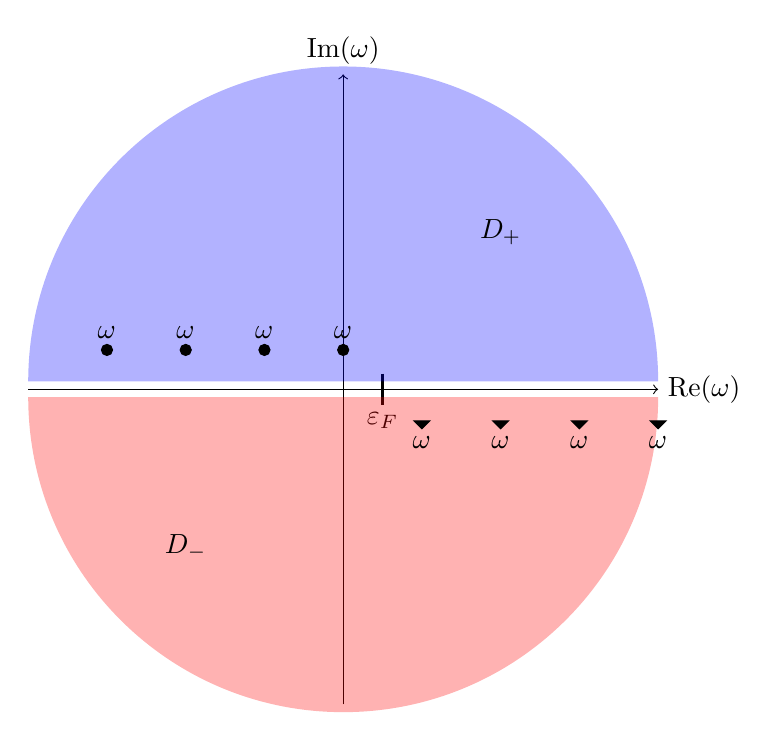
\begin{tikzpicture}
    % Draw the axes
    \draw[->] (-4, 0) -- (4, 0) node[right] {Re($\omega$)};
    \draw[->] (0, -4) -- (0, 4) node[above] {Im($\omega$)};
    
    % Draw the positive real axis label and tick mark for \varepsilon_{F}
    \draw[thick] (0.5, 0.2) -- (0.5, -0.2);
    \node at (0.5, -0.4) {$\varepsilon_{F}$};


    % Draw the semicircle contours
    % fill in its under side
    \fill[blue, opacity=0.3] (4, 0.1) arc[start angle=0, end angle=180, radius=4];
    \fill[red, opacity=0.3] (4, -0.1) arc[start angle=0, end angle=-180, radius=4];
    
    % Draw the poles above the real axis
    \foreach \x in {-3,-2,-1,0} {
        \draw[fill=black] (\x, 0.5) circle (2pt);
    }
    \node at (-3, 0.7) {$\omega_{}$};
    \node at (-2, 0.7) {$\omega_{}$};
    \node at (-1, 0.7) {$\omega_{}$};
    \node at (0, 0.7) {$\omega_{}$};    

    % Draw the poles below the real axis
    \foreach \x in {1,2,3,4} {
        \draw[fill=black] (\x, -0.5) -- ++(0.1, 0.1) -- ++(-0.2, 0) -- cycle;
    }
    \node at (1, -0.7) {$\omega_{}$};
    \node at (2, -0.7) {$\omega_{}$};
    \node at (3, -0.7) {$\omega_{}$};
    \node at (4, -0.7) {$\omega_{}$};

    
    % Label the contours
    \node at (2, 2) {$D_+$};
    \node at (-2, -2) {$D_-$};
    \end{tikzpicture}
    \caption{Contour for the complex frequency integral. The poles are denoted by the various $\omega$. The Fermi energy is denoted by $\varepsilon_F$. The integration contour $D_+$ is the semicircle in the upper complex plane, while $D_-$ is the semicircle in the lower complex plane.}
    \label{fig:contour}
    \end{figure}
\begin{equation}\label{eq:dyson}
    \chi^{\lambda}\left(\mathbf{r}, \mathbf{r}^{\prime}, i \omega\right) = \chi^{0}\left(\mathbf{r}, \mathbf{r}^{\prime}, i \omega\right) 
    + \int d \mathbf{r}_{1} d \mathbf{r}_{2} \chi^{0}\left(\mathbf{r}, \mathbf{r}_{1}, i \omega\right)\left[\frac{\lambda}{\left|\mathbf{r}_{1}-\mathbf{r}_{2}\right|}+f_{\mathrm{xc}}^{\lambda}\left(\mathbf{r}_{1}, \mathbf{r}_{2}, i \omega\right)\right] \chi^{\lambda}\left(\mathbf{r}_{2}, \mathbf{r}^{\prime}, \omega\right)
\end{equation}
where the parameter $\lambda$ controls the amount of interaction in the system, ranging from $\lambda = 0$ for the KS reference system to $\lambda = 1$ for the fully interacting system. The $f_{\mathrm{xc}}^{\lambda}$ is the exchange-correlation kernel, which is set to zero for the RPA. But we will proceed with an RPA calculation anyways in order to solve for the excitation energies and their corresponding eigenvectors. So it makes sense that the numerator of the expression for the screened Coulomb interaction should be given a construction of the ERIs with the excitation factors in a transition density defined as:
\begin{equation}
    w_{pq}^{\mu} = \sum_{ia} (pq|ia) \left(X_{ia}^{\mu} + Y_{ai}^{\mu}\right)
\end{equation}
where we have defined the excitation and de-excitation vectors at the excitation index $\mu$ as $X_{ia}^{\mu}$ and $Y_{ai}^{\mu}$, respectively.
I am not sure how to connect this with the known expression $v\epsilon ^{-1}$; I see the similarities given that we are contracting an ERI with what we get from the RPA calculation that is connected to the polarizability, but can't connect exactly.
We want to figure out how this matches with my previous $O(N^6)$ expression, which was
\begin{equation}
    \Sigma_{pp}^{\text{corr}}(\omega) = \sum_{\mu }^{\text{RPA}}\left(\sum_{i}^{\text{occupied}} \frac{w_{pi}^{\mu }w_{ip}^{\mu }}{\omega -(\epsilon _{i}-\Omega  _{\mu })}+ \sum_{a}^{\text{virtual}} \frac{w_{pa}^{\mu }w_{ap}^{\mu }}{\omega -(\epsilon _{a}+\Omega  _{\mu })}\right)
\end{equation}
for the molecular case. Today I want us to dissect how this equation came about, so that I can understand for my k-point version.
% The expression I get adapted for k-points from GPT is:
% \begin{equation}
% \Sigma_{n n^\prime}^{\text {corr }}(\mathbf{k}, \omega)=\sum_{\mathbf{q}} \sum_\mu^{\text {RPA }}\left(\sum_i^{\text {occupied }} \frac{w_{n i}^\mu(\mathbf{k}, \mathbf{q}) w_{i n^\prime}^\mu(\mathbf{k}-\mathbf{q}, \mathbf{q})}{\omega-\left(\epsilon_{i, \mathbf{k}-\mathbf{q}}-\Omega_{\mu, \mathbf{q}}\right)}+\sum_a^{\text {virtual }} \frac{w_{n a}^\mu(\mathbf{k}, \mathbf{q}) w_{a n^\prime}^\mu(\mathbf{k}-\mathbf{q}, \mathbf{q})}{\omega-\left(\epsilon_{a, \mathbf{k}-\mathbf{q}}+\Omega_{\mu, \mathbf{q}}\right)}\right)
% \end{equation}

\subsection{Analytic continuation}
\label{sec:analytic_continuation}
We start with the original form for the self-energy along the real axis:
\begin{equation}
\Sigma\left(\mathbf{r}, \mathbf{r}^{\prime}, \omega\right)=\frac{i}{2 \pi} \int_{-\infty}^{\infty} d \omega^{\prime} e^{i \omega^{\prime} \eta} G_{0}\left(\mathbf{r}, \mathbf{r}^{\prime}, \omega+\omega^{\prime}\right) W_{0}\left(\mathbf{r}, \mathbf{r}^{\prime}, \omega^{\prime}\right)
\end{equation}
But to avoid the poles, we need to evaluate along the imaginary axis, so the problem becomes:
\begin{equation*}
\Sigma\left(\mathbf{r}, \mathbf{r}^{\prime}, i \omega\right)=-\frac{1}{2 \pi} \int_{-\infty}^{\infty} d \omega^{\prime} G_{0}\left(\mathbf{r}, \mathbf{r}^{\prime}, i \omega+i \omega^{\prime}\right) W_{0}\left(\mathbf{r}, \mathbf{r}^{\prime}, i \omega^{\prime}\right) 
\end{equation*}
We are interested in evaluating the matrix elements of this operator in the molecular orbital basis. Note that both molecular orbitals must have the same crystal momentum in order for it to be conserved in this process. We also apply the identity operator:
\begin{equation}
\bra{n\mathbf{k}} \Sigma (i \omega) \ket{n^\prime\mathbf{k}} = -\frac{1}{2 \pi} \sum_{m\mathbf{k}^\prime}\int_{-\infty}^{\infty} d \omega^{\prime} \bra{n\mathbf{k}} G_0(i \omega + i \omega^{\prime}) \ket{m\mathbf{k^\prime}}\bra{m\mathbf{k^\prime}}W_0(i \omega^{\prime}) \ket{n^\prime\mathbf{k}}
\end{equation}
The noninteracting Green's function has the form:
\begin{equation*}
G_{0}\left(\mathbf{r}, \mathbf{r}^{\prime}, i \omega\right)=\sum_{m \mathbf{k}_{m}} \frac{\psi_{m \mathbf{k}_{m}}(\mathbf{r}) \psi_{m \mathbf{k}_{m}}^{*}\left(\mathbf{r^\prime}\right)}{i \omega+\epsilon_{F}-\epsilon_{m \mathbf{k}_{m}}} \implies G_{0}\left(\mathbf{k} - \mathbf{q}, i \omega + i \omega^{\prime}\right) = \sum_{m \mathbf{k}-\mathbf{q}} \frac{\psi_{m \mathbf{k}-\mathbf{q}} \psi_{m \mathbf{k}-\mathbf{q}}^{*}}{i \left(\omega + \omega^{\prime}\right) + \epsilon_{F} - \epsilon_{m \mathbf{k}-\mathbf{q}}}
\end{equation*}
so that the above equation simplifies to:
\begin{equation}
\boldsymbol{\Sigma}_{n n^{\prime}}(\mathbf{k}, i \omega) = -\frac{1}{2 \pi N_{\mathbf{k}}} \sum_{m \mathbf{q}} \int_{-\infty}^{\infty} d \omega^{\prime} \frac{(n\mathbf{k}, m\mathbf{k}-\mathbf{q} \mid W_0 (\mathbf{q}, i\omega )\mid m \mathbf{k}-\mathbf{q}, n^{\prime}\mathbf{k})}{i \left(\omega + \omega^{\prime}\right) + \epsilon_{F} - \epsilon_{m \mathbf{k}-\mathbf{q}}}
\end{equation}
\subsubsection{Screened Coulomb Interaction}
\begin{align*}
\left(n\mathbf{k}, m\mathbf{k}-\mathbf{q}\left|W_{0}(\mathbf{q}, i\omega )\right| m\mathbf{k}-\mathbf{q}, n^{\prime}\mathbf{k}\right) &= \int \int d \mathbf{r}_1 d \mathbf{r}_2 \psi_{n\mathbf{k}}^{*}(\mathbf{r}_1) \psi_{m\mathbf{k}-\mathbf{q}}(\mathbf{r}_1) W_0(\mathbf{q}, \mathbf{r}_1, \mathbf{r}_2, i\omega ) \psi_{m\mathbf{k}-\mathbf{q}}^{*}(\mathbf{r}_2) \psi_{n^{\prime}\mathbf{k}}(\mathbf{r}_2) \\
\end{align*}
We expand the orbital pair product $\psi_{n \mathbf{k}}^{*}(\mathbf{r}) \psi_{m \mathbf{k}-\mathbf{q}}(\mathbf{r})$ in the auxiliary basis

\begin{equation*}
\psi_{n \mathbf{k}}^{*}(\mathbf{r}) \psi_{m \mathbf{k}-\mathbf{q}}(\mathbf{r})=\sum_{P} b_{P \mathbf{q}}^{n \mathbf{k}, m \mathbf{k}-\mathbf{q}} \phi_{P \mathbf{q}}(\mathbf{r}) 
\end{equation*}
and
\begin{equation}
    \psi_{m\mathbf{k}-\mathbf{q}}^{*}(\mathbf{r}) \psi_{n^{\prime}\mathbf{k}}(\mathbf{r}) = \sum_{Q} b_{Q(-\mathbf{q})}^{m\mathbf{k}-\mathbf{q}, n^{\prime}\mathbf{k}} \phi_{Q(-\mathbf{q})}(\mathbf{r})
\end{equation}
where we have recognized the fact that in the former there is a momentum transfer of $\mathbf{q}$, and in the latter, there is a momentum transfer of $-\mathbf{q}$.
Substituting in gives
\begin{align}
    \left(n\mathbf{k}, m\mathbf{k}-\mathbf{q}\left|W_{0}(\mathbf{q}, i\omega )\right| m\mathbf{k}-\mathbf{q}, n^{\prime}\mathbf{k}\right)\\ = \sum_{PQ} b_{P\mathbf{q}}^{n\mathbf{k}, m\mathbf{k}-\mathbf{q}} \left[\iint d\mathbf{r}_1 d\mathbf{r}_2 \phi_{P\mathbf{q}}(\mathbf{r}_1) W_0(\mathbf{q}, \mathbf{r}_1, \mathbf{r}_2, i\omega ) \phi_{Q(-\mathbf{q})}(\mathbf{r}_2)\right] b_{Q(-\mathbf{q})}^{m\mathbf{k}-\mathbf{q}, n^{\prime}\mathbf{k}}
\end{align}
with

\begin{equation}
b_{P \mathbf{q}}^{n \mathbf{k}, m \mathbf{k}-\mathbf{q}}=\sum_{R}(n \mathbf{k}, m \mathbf{k}-\mathbf{q} \mid R \mathbf{q}) \cdot \mathbf{J}_{R P}^{-1}(\mathbf{q})
\label{eq:nonchol}
\end{equation}
Now is a good place to recall their definition of the density fitting where the ERIs are represented as:


\begin{equation*}
\left(p \mathbf{k}_{p} q \mathbf{k}_{q} \mid r \mathbf{k}_{r} s \mathbf{k}_{s}\right)=\sum_{P Q}\left(p \mathbf{k}_{p} q \mathbf{k}_{q} \mid P \mathbf{k}_{p q}\right) \mathbf{J}_{P Q}^{-1}\left(Q \mathbf{k}_{r s} \mid r \mathbf{k}_{r} s \mathbf{r}_{s}\right), 
\end{equation*}
with
\begin{align*}
\mathbf{J}_{P Q}(\mathbf{k}) & =\iint d \mathbf{r} d \mathbf{r}^{\prime} \phi_{P(-\mathbf{k})}(\mathbf{r}) \frac{1}{\left|\mathbf{r}-\mathbf{r}^{\prime}\right|} \phi_{Q \mathbf{k}}\left(\mathbf{r}^{\prime}\right),  \\
\left(Q \mathbf{k}_{r s} \mid r \mathbf{k}_{r} s \mathbf{k}_{s}\right) & =\iint d \mathbf{r} d \mathbf{r}^{\prime} \phi_{Q \mathbf{k}_{r s}}(\mathbf{r}) \frac{1}{\left|\mathbf{r}-\mathbf{r}^{\prime}\right|} \phi_{r \mathbf{k}_{r}}^{*}\left(\mathbf{r}^{\prime}\right) \phi_{s \mathbf{k}_{s}}\left(\mathbf{r}^{\prime}\right) . 
\end{align*}
Note that these $b$ are then not yet our Cholesky vectors, since each one contains $\frac{|\mathbf{r}-\mathbf{r}^{\prime}|}{|\mathbf{r}-\mathbf{r}^{\prime}|}$ scaling, i.e., there should be a factor of $\mathbf{J}^{-\frac{1}{2}}$  instead of $\mathbf{J}^{-1}$ in \ref{eq:nonchol} if we are to apply the Cholesky vectors.
At this point, we use the expansion of the screened Coulomb interaction:
\begin{align}
    W_0 &= v + v\chi_0 v + v\chi_0 v\chi_0 v + \cdots\\
    &= v(1 + \chi_0 v + \chi_0 v \chi_0 v + \cdots)\\
    &= v^{1/2} \left(1 - \chi_0\right)^{-1} v^{1/2}
\end{align}
simplifying to 
\begin{align}
    \left(n\mathbf{k}, m\mathbf{k}-\mathbf{q}\left|W_{0}(\mathbf{q}, i\omega )\right| m\mathbf{k}-\mathbf{q}, n^{\prime}\mathbf{k}\right) &= \sum_{PQ} b_{P\mathbf{q}}^{n\mathbf{k}, m\mathbf{k}-\mathbf{q}} \left[\mathbf{J^{\frac{1}{2}}}\left( \mathbf{I} - \boldsymbol{\Pi}(\mathbf{q}, i\omega ) \right) \mathbf{J^{\frac{1}{2}}}\right]^{-1}_{PQ} b_{Q(-\mathbf{q})}^{m\mathbf{k}-\mathbf{q}, n^{\prime}\mathbf{k}}\\
    &= \sum_{PQ} v_{P}^{n m}\left[\mathbf{I}-\mathbf{\Pi}\left(\mathbf{q}, i \omega^{\prime}\right)\right]_{P Q}^{-1} v_{Q}^{m n^{\prime}}
\end{align}
where $\mathbf{J}_{PQ}$ is the Coulomb interaction projected onto the auxiliary basis, and we have defined
\begin{equation}
    v_{P\mathbf{q}}^{n \mathbf{k}, m \mathbf{k}-\mathbf{q}} = \sum_{pq} C_{pn}(\mathbf{k}) C_{qm}(\mathbf{k}-\mathbf{q}) v_{P\mathbf{q}}^{p\mathbf{k}, q\mathbf{k}-\mathbf{q}}
\label{eq:mochol}
\end{equation}
with
\begin{equation}
    v_{P\mathbf{q}}^{p\mathbf{k}, q\mathbf{k}-\mathbf{q}} = \sum_R (p\mathbf{k}, q\mathbf{k}-\mathbf{q} \mid R\mathbf{q}) \mathbf{J}_{RP}^{-1/2}(\mathbf{q})
\end{equation}
If we first rename $\mathbf{k^\prime} = \mathbf{k}-\mathbf{q} \implies \mathbf{k} = \mathbf{k^\prime} + \mathbf{q}$, and then we are free to redefine $\mathbf{q} \rightarrow -\mathbf{q}$, so that \ref{eq:mochol} becomes
\begin{equation}
    v_{P\mathbf{-q}}^{n \mathbf{k}-\mathbf{q}, m \mathbf{k}} = \sum_{pq} C_{pn}(\mathbf{k}-\mathbf{q}) C_{qm}(\mathbf{k}) v_{P\mathbf{-q}}^{p\mathbf{k}-\mathbf{q}, q\mathbf{k}}
\end{equation}
but we know that the bare Coulomb potential projected onto the auxiliary basis is given by
\begin{equation}
    v_{P\mathbf{q}}^{n\mathbf{k}, m\mathbf{k}-\mathbf{q}} = \sum_{pq} C_{pn}(\mathbf{k}) C_{qm}(\mathbf{k}-\mathbf{q}) v_{P\mathbf{q}}^{p\mathbf{k}, q\mathbf{k}-\mathbf{q}}
\end{equation}

To ease notation, some momentum labels are suppressed in the above and following equations (e.g., we will use $b_{P}^{n m}$ to denote $b_{P \mathbf{q}}^{n \mathbf{k}, m \mathbf{k}-\mathbf{q}}$ ). Using Eqs. 19-21, the matrix elements of $W_{0}$ are computed as

\begin{align*}
& \left(n \mathbf{k}, m \mathbf{k}-\mathbf{q}\left|W_{0}\right| m \mathbf{k}-\mathbf{q}, n^{\prime} \mathbf{k}\right) \\
& =\sum_{P Q} b_{P}^{n m}\left[\iint d \mathbf{r} d \mathbf{r}^{\prime} \phi_{P \mathbf{q}}(\mathbf{r}) W_{0}\left(\mathbf{r}, \mathbf{r}^{\prime}, i \omega^{\prime}\right) \phi_{Q(-\mathbf{q})}\left(\mathbf{r}^{\prime}\right)\right] b_{Q}^{m n^{\prime}} \\
& =\sum_{P Q} b_{P}^{n m}\left[\mathbf{J}_{P Q}(\mathbf{q})+\left(\mathbf{J}^{1 / 2} \boldsymbol{\Pi} \mathbf{J}^{1 / 2}\right)_{P Q}(\mathbf{q})+\ldots\right] b_{Q}^{m n^{\prime}}  \\
& =\sum_{P Q} v_{P}^{n m}\left[\mathbf{I}-\mathbf{\Pi}\left(\mathbf{q}, i \omega^{\prime}\right)\right]_{P Q}^{-1} v_{Q}^{m n^{\prime}}
\end{align*}

The 3-center 2-electron integral $v_{P}^{n m}$ between auxiliary basis function $P$ and molecular orbital pairs $n m$ is obtained from an AO to MO transformation of the GDF AO integrals defined in Eq. 15:

\begin{equation*}
v_{P}^{n m}=\sum_{p} \sum_{q} C_{p n}(\mathbf{k}) C_{q m}(\mathbf{k}-\mathbf{q}) v_{P \mathbf{q}}^{p \mathbf{k}, q \mathbf{k}-\mathbf{q}} 
\end{equation*}

where $C(\mathbf{k})$ refers to the MO coefficients in the AO basis. $\Pi\left(\mathbf{q}, i \omega^{\prime}\right)$ in Eq. 22 is an auxiliary density response function:

\begin{equation*}
\boldsymbol{\Pi}_{P Q}\left(\mathbf{q}, i \omega^{\prime}\right)=\frac{2}{N_{\mathbf{k}}} \sum_{\mathbf{k}} \sum_{i}^{\mathrm{occ}} \sum_{a}^{\text {vir }} v_{P}^{i a} \frac{\epsilon_{i \mathbf{k}}-\epsilon_{a \mathbf{k}-\mathbf{q}}}{\omega^{\prime 2}+\left(\epsilon_{i \mathbf{k}}-\epsilon_{a \mathbf{k}-\mathbf{q}}\right)^{2}} v_{Q}^{a i} 
\end{equation*}
\section{UHF formalism}
The first thing to do is to solve the Casida equation for the polarizability in the direct formulation of the RPA:
\begin{equation}\label{eq:kptsCasida}
	\begin{pmatrix}
        \mathbf{A}  & \mathbf{B} \\
        \mathbf{B}^{*} & \mathbf{A}^{*}
    \end{pmatrix}
    \begin{pmatrix}
        \mathbf{X} \\
        \mathbf{Y}
    \end{pmatrix}
    =
    \begin{pmatrix}
        \Omega & 0 \\
        0 & -\Omega
    \end{pmatrix}
    \begin{pmatrix}
        \mathbf{X} \\
        \mathbf{Y}
    \end{pmatrix}
\end{equation}
with $\mathbf{A}$ and $\mathbf{B}$ given by
    \begin{align}\nonumber
    \mathbf{A}_{ia, jb}^{\sigma \sigma ^{\prime}} &= \delta_{ij}\delta_{ab}\delta_{\sigma \sigma ^{\prime}}(\varepsilon_a - \varepsilon_i) + (i_{\sigma}a_{\sigma}|b_{\sigma ^{\prime}}j_{\sigma ^{\prime}}) \\
    \mathbf{B}_{ia, jb}^{\sigma \sigma ^{\prime}} &= (i_{\sigma}a_{\sigma}|j_{\sigma ^{\prime}}b_{\sigma ^{\prime}})
\end{align}
Therefore, with the different spins we form a super matrix:
\begin{equation}
    \begin{pmatrix}
\begin{pmatrix}
    \mathbf{A}_{\alpha \alpha } & \mathbf{A}_{\alpha \beta } \\
    \mathbf{A}_{\beta \alpha } & \mathbf{A}_{\beta \beta }
\end{pmatrix}
&
\begin{pmatrix}
    \mathbf{B}_{\alpha \alpha } & \mathbf{B}_{\alpha \beta } \\
    \mathbf{B}_{\beta \alpha } & \mathbf{B}_{\beta \beta }
\end{pmatrix}
\\
\begin{pmatrix}
    \mathbf{B}_{\alpha \alpha }^{*} & \mathbf{B}_{\alpha \beta }^{*} \\
    \mathbf{B}_{\beta \alpha }^{*} & \mathbf{B}_{\beta \beta }^{*}
\end{pmatrix}
&
\begin{pmatrix}
    \mathbf{A}_{\alpha \alpha }^{*} & \mathbf{A}_{\alpha \beta }^{*} \\
    \mathbf{A}_{\beta \alpha }^{*} & \mathbf{A}_{\beta \beta }^{*}
\end{pmatrix}
\end{pmatrix}
    \begin{pmatrix}
        \mathbf{X}_{\alpha\alpha} & \mathbf{X}_{\alpha\beta}\\
        \mathbf{X}_{\beta\alpha} & \mathbf{X}_{\beta\beta}\\
        \mathbf{Y}_{\alpha\alpha} & \mathbf{Y}_{\alpha\beta}\\
        \mathbf{Y}_{\beta\alpha} & \mathbf{Y}_{\beta\beta}
    \end{pmatrix}
    =
    \begin{pmatrix}
        \Omega & 0 & 0 & 0\\
        0 & \Omega & 0 & 0\\
        0 & 0 & -\Omega & 0\\
        0 & 0 & 0 & -\Omega
    \end{pmatrix}
    \begin{pmatrix}
        \mathbf{X}_{\alpha\alpha} & \mathbf{X}_{\alpha\beta}\\
        \mathbf{X}_{\beta\alpha} & \mathbf{X}_{\beta\beta}\\
        \mathbf{Y}_{\alpha\alpha} & \mathbf{Y}_{\alpha\beta}\\
        \mathbf{Y}_{\beta\alpha} & \mathbf{Y}_{\beta\beta}
    \end{pmatrix}
\end{equation}
Now, there will be $2OV$ unique excitation energies; we sort them into singlets or triplets as follows: for each excitation we compute the overlap between the $\alpha $ and $\beta $ excitation. For TDA, this is just the $\nu$th column of $\begin{pmatrix}
\mathbf{X}_{\alpha\alpha} & \mathbf{X}_{\alpha\beta}\\
\end{pmatrix}$ with the $\nu$th row of $\begin{pmatrix}
    \mathbf{X}_{\beta\alpha} \\ \mathbf{X}_{\beta\beta}\\
\end{pmatrix}$. If greater than 0, we have a singlet excitation, otherwise we have a triplet excitation. For later use in GW, we just want the neutral excitation energies, so we only care about the singlet excitations.
% This implies a way to get the excitation energies $\Omega^\mu$ and the eigenvectors $\mathbf{X}^\mu$ and $\mathbf{Y}^\mu$ for a certain spin channel $\sigma $. Next, for each spin channel, we need to formulate the matrix $\mathbf{M}^{\mu }$, which is used to form the transition densities.
% \begin{equation}
% M_{i a j b}^{\mu }=X_{i a}^{\mu } X_{j b}^{\mu }+X_{i a}^{\mu } Y_{j b}^{\mu }+Y_{i a}^{\mu } X_{j b}^{\mu }+Y_{i a}^{\mu } Y_{j b}^{\mu }
% \end{equation}
% With these quantities, we can then form the self energy for the given spin channel:
% \begin{equation}
% \Sigma_{p q}^c\left(\omega \right)= \sum_{j b k c} \sum_{\mu }\left(\sum_i \frac{(i p \mid j b)(i q \mid k c)}{\omega -\Omega_{\mu }-\varepsilon_i^{\mathrm{MF}}-\mathrm{i} \eta}\right.
% \left.+\sum_a \frac{(a p \mid j b)(a q \mid k c)}{\omega +\Omega_{\mu }-\varepsilon_a^{\mathrm{MF}}+\mathrm{i} \eta}\right) M_{j b k c}^{\mu }
% \label{eq:Sigma}
% \end{equation}
% But in solving the case partial equation, we are just interested in the real, diagonal part of the self energy, so this reduces to:
% \begin{equation}
% \Sigma_{p p}^c\left(\omega \right)= \sum_{j b k c} \sum_{\mu }\left(\sum_i \frac{(i p \mid j b)(i p \mid k c)}{\omega -\Omega_{\mu }-\varepsilon_i^{\mathrm{MF}}} + \sum_a \frac{(a p \mid j b)(a p \mid k c)}{\omega +\Omega_{\mu }-\varepsilon_a^{\mathrm{MF}}}\right) M_{j b k c}^{\mu }
% \end{equation}

\section{Deriving linear response: 11/22}
\subsection{The Fundamentals}
The motivation for this is to be able to understand why the poles of the screened Coulomb interaction are the same as those of the fully interacting polarizability, which are given by the frequencies of the RPA, obtained by diagonalizing the Casida equation. And then we want to be able to connect why $W_0 = v + v\chi_0 v + \ldots = \frac{v}{1-\chi_0 v}$ where $W_0$ is the screened Coulomb interaction and $\chi_0$ is the non-interacting polarizability with Lehmann representation. 
\begin{equation}
    \chi_{0}\left(\mathbf{r}, \mathbf{r}^{\prime}, \omega\right)=\sum_{ia}\frac{\psi_{i}(\mathbf{r}) \psi_{a}^{*}(\mathbf{r}^{\prime}) \psi_{i}(\mathbf{r}^{\prime}) \psi_{a}^{*}(\mathbf{r})}{\omega-\left(\epsilon_{a}-\epsilon_{i}\right)+i \eta \operatorname{sgn}\left(\epsilon_{a}-\epsilon_{i} - \mu\right)}
\end{equation}
to do so, one must understand the reformulation of based on the density matrix as for posed by Furche \cite{furche2001density}.
Alternatively, let us start from the known Dyson equation that relates the fully interacting Green's function to the non-interacting one. We know the integral form of the Dyson equation is
\begin{equation}
    G(1,2) = G_0(1,2) + \int d3 d4 G_0(1,3) \Sigma(3,4) G(4,2)
\end{equation}
but we proceed symbolically to get
\begin{align}
    G &= G_0 + G_0 \Sigma G \\
    \left(I - G_0 \Sigma\right) G &= G_0 \\
    G &= \left(I - G_0 \Sigma\right)^{-1} G_0 \\
    G &= \left(G_0\left(G_0^{-1} - \Sigma \right)\right)^{-1} G_0 \\
    G &= \left(G_0^{-1} - \Sigma \right)^{-1}
\end{align}
Now, we also know the Dyson equation for the polarizability is
\begin{equation}
    \begin{aligned}
\chi\left(\omega, x_1, x_2\right)= & \chi_0\left(\omega, x_1, x_2\right)+\int d x d x^{\prime} \chi_0\left(\omega, x_1, x\right) \\
& \times\left(\frac{1}{\left|\mathbf{r}-\mathbf{r}^{\prime}\right|}+f_{\mathrm{xc}}\left(\omega, x, x^{\prime}\right)\right) \chi\left(\omega, x^{\prime}, x_2\right)
\end{aligned}
\end{equation}
In the RPA, we neglect the exchange correlation kernel $f_{\text{xc}}$, so we have
\begin{equation}
    \chi_{RPA} = \chi_0 + \chi_0 v \chi_{RPA} = \frac{\chi_0}{1 - v \chi_0}
\end{equation}
where in the final step we used the symbolic manipulation that was used before. So $W_0 = \frac{v}{1 - v \chi_0} = v\chi_{RPA}\chi_0^{-1} = v\left(\frac{\chi_0 \chi_0^{-1}}{1 - v \chi_0}\right) = \frac{v}{1 - v \chi_0}$. Therefore, we see why the poles of $W_0$ are the same as those of $\chi_{RPA}$, since they have a linear relationship. Now, we will proceed to derive the poles of $\chi_{RPA}$. But first we must introduce the density matrix based linear response theory.

\subsection{Introduction to TDKS}


In time-dependent density functional theory (TDDFT), the \textbf{Time-Dependent Kohn-Sham (TDKS)} equations describe a system of $N$ noninteracting fermions that reproduce the same time-dependent density $\rho(t, \mathbf{r})$ as the interacting system. The TDKS equations are given by:

\begin{equation}
i \frac{\partial}{\partial t} \varphi_{j}(t, \mathbf{r}) = H[\rho](t, \mathbf{r}) \varphi_{j}(t, \mathbf{r}) \label{eq:TDKS}
\end{equation}
where \( j = 1, \ldots, N \) indexes the Kohn-Sham orbitals \( \varphi_{j}(t, \mathbf{r}) \), and \( H[\rho](t, \mathbf{r}) \) is the effective one-particle Hamiltonian defined as:

\begin{equation}
H[\rho](t, \mathbf{r}) = \frac{\boldsymbol{\pi}^2(t, \mathbf{r})}{2} + v_{\text{eff}}[\rho](t, \mathbf{r}) \label{eq:HKohnSham}
\end{equation}

where $v_{\text{eff}}[\rho](t, \mathbf{r}) = v_{\text{ext}}(t, \mathbf{r}) + v_{\text{H}}[\rho](t, \mathbf{r}) + v_{\text{xc}}[\rho](t, \mathbf{r})$.


The operator \( \boldsymbol{\pi}(t, \mathbf{r}) \) is known as the \textbf{kinetic momentum operator}. In the presence of an electromagnetic field, the kinetic momentum operator is modified from the canonical momentum operator \( \mathbf{p} \) to include the effects of the vector potential \( \mathbf{A}_{\text{ext}}(t, \mathbf{r}) \):

\begin{equation}
\boldsymbol{\pi}(t, \mathbf{r}) = \mathbf{p} + \frac{1}{c} \mathbf{A}_{\text{ext}}(t, \mathbf{r}) \label{eq:kineticMomentum}
\end{equation}

Here, \( \mathbf{p} = -i\hbar \nabla \) is the canonical momentum operator, and \( c \) is the speed of light. The vector potential \( \mathbf{A}_{\text{ext}}(t, \mathbf{r}) \) accounts for the influence of external perturbative electromagnetic fields on the system. \emph{Why it does the influence of the vector potential not just all go into the $v_{\text{eff}}$?}

But we know that under a gauge transformation, the physical observables will be invariant, while the orbits will merely acquire a \textbf{phase factor}:

\begin{equation}
\varphi_{j}(t, \mathbf{r}) \rightarrow \varphi'_{j}(t, \mathbf{r}) = \varphi_{j}(t, \mathbf{r}) \exp\left(-\frac{i}{c} \psi(t, \mathbf{r})\right) \label{eq:phaseFactor}
\end{equation}
Therefore observables, like the density or current density will be unaffected by this gauge transformation.


\subsection{Density Matrix Formulation in TDKS Theory}

In Time-Dependent Density Functional Theory (TDDFT), the \textbf{Time-Dependent Kohn-Sham (TDKS)} equations \ref{eq:TDKS} describe a system of $N$ noninteracting fermions that reproduce the same time-dependent electron density $\rho(t, \mathbf{r})$ as the interacting system. An alternative formulation of TDKS theory utilizes the one-particle density matrix $\gamma(t, \mathbf{r}, \mathbf{r}')$, which offers advantage because it introduces a basis that one can exploit computationally.
The one-particle density matrix is defined as:
\begin{equation}
\gamma(t, \mathbf{r}, \mathbf{r}') = \sum_{j=1}^{N} \varphi_{j}(t, \mathbf{r}) \varphi_{j}^{*}(t, \mathbf{r}') 
\label{eq:densityMatrix}
\end{equation}
and it is idempotent, meaning that
\begin{equation}
\gamma^{2}(t, \mathbf{r}, \mathbf{r}') = \gamma(t, \mathbf{r}, \mathbf{r}') \end{equation}
See section \ref{sec:density_matrix_idempotency} for a proof.





Now, we would like to derive an evolution equation for the density matrix in analogy with the one we already have for the KS orbitals in equation \ref{eq:TDKS}. The result is
\begin{equation}
i \frac{\partial}{\partial t} \gamma(t) = \left[ H[\rho](t), \gamma(t) \right] 
\label{eq:densityMatrixTD}
\end{equation}
See section \ref{sec:densityMatrixTD} for proof.
For the purposes of response theory, it is convenient to consider external scalar potentials,


\begin{equation}
v_{\mathrm{ext}}(t, x)= v^{(0)}(x)+\sum_{\alpha} \lambda_{\alpha}\left(v^{(\alpha)}\left(\omega_{\alpha}, x\right) e^{i \omega_{\alpha} t}+v^{(\alpha)}\left(-\omega_{\alpha}, x\right) e^{-i \omega_{\alpha} t}\right)
\end{equation}
and longitudinal vector potentials


\begin{equation}
\mathbf{A}_{\mathrm{ext}}(t, x)= \sum_{\alpha} \lambda_{\alpha}\left(\mathbf{A}^{(\alpha)}\left(\omega_{\alpha}, x\right) e^{i \omega_{\alpha} t}+\mathbf{A}^{(\alpha)}\left(-\omega_{\alpha}, x\right) e^{-i \omega_{\alpha} t}\right)
\end{equation}
Note that we are not considering transverse vector potentials, as we would get if we had a magnetic field. The cemetery of the Fourier component is fate in section \ref{sec:FourierTransformSymmetry}. Next, we need to determine the derivatives of the observables with respect to a perturbation. We have
Any time-dependent expectation value $f_{\lambda}(t)$ is a function of the coupling strength vector $\boldsymbol{\lambda}$. Its response to the external perturbation is defined by its derivatives with respect to $\boldsymbol{\lambda}$ at $\boldsymbol{\lambda}=0$. For monochromatic perturbations, the derivatives exhibit a characteristic time dependence,


\begin{align}
& \left.f_{\lambda}(t)\right|_{\boldsymbol{\lambda}=0}=f^{(0)},  \\
& \left.\frac{\partial}{\partial \lambda_{\alpha}} f_{\lambda}(t)\right|_{\boldsymbol{\lambda}=0}=f^{(\alpha)}\left(\omega_{\alpha}\right) e^{i \omega_{\alpha} t}+f^{(\alpha)}\left(-\omega_{\alpha}\right) e^{-i \omega_{\alpha} t},  \\
\end{align}
Proof of the second expression is given in section \ref{sec:firstOrderResponse}. The third expression follows by taking the derivative of the second expression.
\begin{align}
    \left.\frac{\partial^{2}}{\partial \lambda_{\alpha} \partial \lambda_{\beta}} f_{\lambda}(t)\right|_{\boldsymbol{\lambda}=0}&= f^{(\alpha \beta)}  \left(\omega_{\alpha}, \omega_{\beta}\right) e^{i\left(\omega_{\alpha}+\omega_{\beta}\right) t} + f^{(\alpha \beta)}  \left(\omega_{\alpha}, -\omega_{\beta}\right) e^{i\left(\omega_{\alpha}-\omega_{\beta}\right) t}\\
 &+ f^{(\alpha \beta)}  \left(-\omega_{\alpha}, \omega_{\beta}\right) e^{i\left(-\omega_{\alpha}+\omega_{\beta}\right) t} + f^{(\alpha \beta)}  \left(-\omega_{\alpha}, -\omega_{\beta}\right) e^{-i\left(\omega_{\alpha}+\omega_{\beta}\right) t}
\end{align}
These expressions define the frequency dependent response of $f_{\lambda}$ up to second order. The key step is to realize that when evaluating the expectation value of some observable $O$, we must consider the coupling to the density matrix, i.e. $f_{\lambda}(t)=\operatorname{tr}\left(O(t) \gamma_{\lambda}(t)\right)$.
 
The route to frequency-dependent response properties is then obvious: (1) Calculate the frequencydependent KS density matrix response by differentiation of Eqs. (8) and (10); (2) Take the trace with $O$. The interacting response can be calculated from the noninteracting KS system because the TDKS density matrix yields the interacting density and current density as it follows from Eq. (9). \textbf{Better understanding needed.}

For the idempotency constraint, expansion up to second order yields, in shorthand notation,


\begin{align*}
& \gamma^{(0)}=\gamma^{(0)} \gamma^{(0)},  \tag{16}\\
& \gamma^{(\alpha)}=\gamma^{(0)} \gamma^{(\alpha)}+\gamma^{(\alpha)} \gamma^{(0)},  \tag{17}\\
& \gamma^{(\alpha \beta)}=\gamma^{(0)} \gamma^{(\alpha \beta)}+\gamma^{(\alpha)} \gamma^{(\beta)}+\gamma^{(\beta)} \gamma^{(\alpha)}+\gamma^{(\alpha \beta)} \gamma^{(0)} . \tag{18}
\end{align*}


The equations of motion up to second order read
\begin{align}
0 &=\left[H^{(0)}, \gamma^{(0)}\right] \\
\omega_{\alpha} \gamma^{(\alpha)}& =\left[H^{(0)}, \gamma^{(\alpha)}\right]+\left[H^{(\alpha)}, \gamma^{(0)}\right]\\
\left(\omega_{\alpha}+\omega_{\beta}\right) \gamma^{(\alpha \beta)}& = {\left[H^{(0)}, \gamma^{(\alpha \beta)}\right]+\left[H^{(\alpha)}, \gamma^{(\beta)}\right] } +\left[H^{(\beta)}, \gamma^{(\alpha)}\right]+\left[H^{(\alpha \beta)}, \gamma^{(0)}\right]
\end{align}
Proof of this series is given in section \ref{sec:firstOrderIdempotency}. 
\section{GW Density Matrix}
The expression for the density matrix $\gamma $ is
\begin{equation}
\gamma\left(\mathbf{r}, \mathbf{r}^{\prime}\right)=-\frac{i}{2 \pi} \int_{-\infty}^{+\infty} d \omega e^{i \eta \omega} G\left(\mathbf{r}, \mathbf{r}^{\prime}, \omega\right)
\end{equation}
Next, we want to consider the expression for the linearized Dyson equation, which is given by
\begin{equation}
G=G_0+G_0\left(\Sigma_{x c}-V_{x c}\right) G_0
\label{eq:linearDyson}
\end{equation}
So by inserting this LDE into the expression for the density matrix, we can identify a few different terms. First, consider the term just corresponding to $G_0$:
\begin{equation}
\gamma_{\mathbf{k} i j}^{\mathrm{gKS}}=2 \delta_{i j} \theta\left(\mu-\epsilon_{\mathbf{k} i}\right)
\end{equation}
We can take a similar approach to treat the static portion of \ref{eq:linearDyson}, i.e., the Hartree-Fock term, which is given by
\begin{equation}
\Delta \gamma_{\mathbf{k} i j}^{\mathrm{HF}}=2 \theta\left(\mu-\epsilon_{\mathbf{k} i}\right) \theta\left(\epsilon_{\mathbf{k} j}-\mu\right) \frac{\langle\mathbf{k} i| \Sigma_x-V_{xc}|\mathbf{k} j\rangle}{\epsilon_{\mathbf{k} i}-\epsilon_{\mathbf{k} j}}
\end{equation}
Note that for a HF noninteracting Green's function, the static term is given by the Hartree-Fock self-energy, but this cancels out exactly with the exchange correlation potential $V_{xc}$, so this term is zero. Finally we have the most complicated term involving the insertion of $G_0\Sigma _c G_0$. The correlation self energy has a frequency dependence, so what they do is
Finally, we get
\begin{equation}
\gamma^{G W}=\gamma^{\mathrm{gKS}}+\Delta \gamma^{\mathrm{HF}}+\Delta \gamma^{G W}
\end{equation}
% A similar approach can be used for the static term right-hand part of Eq. (4), $G_0\left(\Sigma_x-V_{x c}\right) G_0$ :
% $$
% \Delta \gamma_{\mathbf{k} i j}^{\mathrm{HF}}=2 \theta\left(\mu-\epsilon_{\mathbf{k} i}\right) \theta\left(\epsilon_{\mathbf{k} j}-\mu\right) \frac{\langle\mathbf{k} i| \Sigma_x-V_{x c}|\mathbf{k} j\rangle}{\epsilon_{\mathbf{k} i}-\epsilon_{\mathbf{k} j}}
% $$
\chapter{Dyson to GQME: 12/13}



The Generalized Quantum Master Equation (GQME) is given by
\begin{equation}
\dot{\mathcal{C}}(t) = \mathcal{C}(t) {\Omega_1} - \int_{0}^{t} d \tau\, \mathcal{C}(t - \tau) \mathcal{K}_1(\tau) + D(t)
\label{eq:GQME}
\end{equation}
where the correlation function is defined as 
\begin{equation}
    \mathcal{C}(t) = (\hat{{\mu}} \mid \hat{{\mu}}(t)),
\label{eq:C}
\end{equation}
the higher-order moments are
\begin{equation}
\Omega_{n} \equiv\left((i \mathcal{L})^{n} \hat{{\mu}}, \hat{{\mu}}\right) /(\hat{{\mu}}, \hat{{\mu}})
\end{equation}
with the auxiliary kernels
\begin{equation}
K_{n}(t) \equiv\left((i \mathcal{L})^{n} \hat{f}(t), \hat{{\mu}}\right) /(\hat{{\mu}}, \hat{{\mu}})
\end{equation}
$\hat{f}(t)$ in the above equation is referred to as the random force operator
\begin{equation}
\hat{f}(t) \equiv e^{i t {\mathcal { L }} \mathcal{L}} \mathcal{Q} i \mathcal{L} \hat{{\mu}}
\end{equation}
with $\mathcal{Q}={\mathcal { I }}-\mathcal{P}$ being the complementary projection operator. But this becomes complicated, so Wenjie found that we can express $\mathcal{K}_1(t)$ without time evolution using $\hat{f}(0)=\mathcal{Q} i \mathcal{L} \hat{\mu}$ and, we get
\begin{equation}
K_{n}(0)=\Omega_{n+1}-\Omega_{n} \Omega_{1}
\end{equation}
Therefore, we only need to consider $\dot{K}_{1}(t)$, which can be obtained directly:
\begin{equation}
\dot{K}_{1}(t)=\frac{(i \mathcal{L} \dot{\hat{f}}(t), \hat{\mu})}{(\hat{\mu}, \hat{\mu})}=K_{2}(t)-\Omega_{1} K_{1}(t)
\end{equation}
Similarly, we can show that the auxiliary kernels are coupled through
\begin{equation}
\dot{K}_{n}(t)=K_{n+1}(t)-\Omega_{n} K_{1}(t).
\end{equation}
We expect that the higher order auxiliary kernels will decay quickly, so we can truncate the series at some finite $n$.
The moments of the memory kernel are
\begin{equation}
    \Omega_n = \frac{ \left( (i \mathcal{L})^{n} \hat{{\mu}}, \hat{{\mu}} \right) }{ (\hat{{\mu}}, \hat{{\mu}}) },
\label{eq:Omega}
\end{equation}
with $\mathcal{L}$ being the Liouville superoperator with $\mathcal{L} \hat{{\mu}} = \left[ \hat{H}, \hat{{\mu}} \right]$. The construction of the numerator in equation \ref{eq:Omega} can be thought of as the generation of a Krylov subspace up to level $n$, i.e. we need to build up $\mathcal{K}_n(\mathcal{L}, \hat{{\mu}})= \text{span}\{\hat{{\mu}}, (i\mathcal{L})\hat{{\mu}}, (i\mathcal{L})^2\hat{{\mu}},\ldots, (i\mathcal{L})^{n-1}\hat{{\mu}}\}$, where $\hat{{\mu}} = \hat{c}$ or $\hat{c}^{\dagger}$. In the case if we choose $\hat{{\mu}}=\hat{c}$, we get the lesser Green's function 
\begin{equation}
\mathcal{C}(t) = (\hat{c}, \hat{c}(t)) \equiv \langle \hat{c}^{\dagger}(0)\hat{c}(t)\rangle = \frac{G^<(t)}{i}
\end{equation}
whereas if we chose $\hat{{\mu}}=\hat{c}^{\dagger}$, we get the greater Green's function 
\begin{equation}
\mathcal{C}(t) = (\hat{c}^{\dagger}, \hat{c}^{\dagger}(t)) \equiv \langle \hat{c}(0)\hat{c}^{\dagger}(t)\rangle = -\frac{G^>(t)}{i}
\end{equation}
Then we can construct the retarded Green's function as
\begin{equation}
    G_R(t) = \Theta(t) \left( G^<(t) - G^>(t) \right)
\end{equation}
Using Krylov subspace methods, one never has to construct the Liouvillian matrix, but instead can directly compute the extremal eigenvalues and eigenvectors of $\mathcal{L}$ by considering the action of $\mathcal{L}$ on the Krylov subspace.

\section{Explicit Construction of the Liouville Superoperator}
Consider that we are working with the upfolded Hamiltonian
\begin{equation}
    \textbf{H} = \begin{pmatrix}
        \textbf{f} & \textbf{W} \\
        \textbf{W}^{\dagger} & \textbf{d}
    \end{pmatrix}
\end{equation}
where we again have a physical space $\textbf{f}$ and a bath space $\textbf{d}$,  whose coupling is given by $\textbf{W}$. Tell me what would happened if we considered the action of this on the composite operator vector defined lower?
Lets consider making a Krylov subspace, corresponding to repeated applications of the Liouville superoperator to the initial operator $\hat{\boldsymbol{\mu}}$.
 Now, The idea is to define a composite operator vector
\begin{equation}
\hat{\boldsymbol{\mu}} \equiv
\begin{pmatrix}
\hat{\mu}_1 \\
\hat{\mu}_2
\end{pmatrix} = \begin{pmatrix}
\hat{c} \\
\hat{c}^{\dagger}
\end{pmatrix},
\end{equation}
where \( \hat{c} \) is the annihilation operator and \( \hat{c}^{\dagger} \) is the creation operator. Notice that the equation of motion for the Green's function is
\begin{align}
(i \partial_t - \hat{H}_0) G(t,t') = \delta(t-t') 
+ \int_{-\infty}^{\infty} d\tau \, \Sigma(t,\tau) \, G(\tau,t')\\ \rightarrow \dot{G(t,t')} = -i \hat{H}_0 G(t,t') -i\delta(t-t') + \int_{-\infty}^{\infty} d\tau' \, \Sigma(t,\tau') \, G(\tau',t')
\end{align}
So our task becomes to figure out how 
\begin{equation}
    -i \hat{H}_0 G(t,t') -i\delta(t-t') + \int_{-\infty}^{\infty} d\tau' \, \Sigma(t,\tau') \, G(\tau',t') = \mathcal{C}(t) {\Omega_1} - \int_{0}^{t} d \tau\, \mathcal{C}(t - \tau) \mathcal{K}(\tau) + D(t)
\end{equation}
I feel like it should be the case that $-i \hat{H}_0 G(t,t')= \mathcal{C}(t) {\Omega_1}$. Do you think that this should be the case or no? Because I think we can agree that the equation that comes first should be the same as the equation of motion for the greens function. And then try to apply a decomposed Hamiltonia like $H=H_0+V$ to the first equation, so that we can see what happens.



To simple by things as much as possible initially consider that we only use the noninteracting Hamiltonian $\hat{H}_0= \epsilon \hat{c}^\dagger \hat{c}$ in the action of the Liouvillian.
\begin{equation}
    \Omega_1 = \frac{ \left( (i \mathcal{L}) \hat{\boldsymbol{\mu}}, \hat{\boldsymbol{\mu}} \right) }{ (\hat{\boldsymbol{\mu}}, \hat{\boldsymbol{\mu}}) } = \frac{ \left( (i [\hat{H}_0, \hat{\boldsymbol{\mu}}], \hat{\boldsymbol{\mu}} \right) }{ (\hat{\boldsymbol{\mu}}, \hat{\boldsymbol{\mu}}) }
\end{equation}
If we just consider the numerator, we see that
\begin{equation}
    \left( (i [\hat{H}_0, \hat{\boldsymbol{\mu}}], \hat{\boldsymbol{\mu}} \right) = \left( i [\hat{H}_0, \hat{c}], \hat{c} \right) + \left( i [\hat{H}_0, \hat{c}^\dagger], \hat{c}^\dagger \right)
\end{equation}
Considering just the first term
\begin{equation}
    \left( i [\hat{H}_0, \hat{c}], \hat{c} \right) = -i \epsilon ([\hat{c}^\dagger \hat{c}, \hat{c}] , \hat{c}) = -i \epsilon (\hat{c}, \hat{c}) = -i \epsilon\left(1-f(\epsilon)\right)
\end{equation}
and the second term
\begin{equation}
    \left( i [\hat{H}_0, \hat{c}^\dagger], \hat{c}^\dagger \right) = -i \epsilon ([\hat{c}^\dagger \hat{c}, \hat{c}^\dagger] , \hat{c}^\dagger) = -i \epsilon (\hat{c}^\dagger, \hat{c}^\dagger) = -i \epsilon f(\epsilon)
\end{equation}
which can be summarized as
\begin{equation}
    \left( i [\hat{H}_0, \hat{\boldsymbol{\mu}}], \hat{\boldsymbol{\mu}} \right) = -i \epsilon \implies \Omega_1 = -i \epsilon
\label{eq:Omega1}
\end{equation}
Now, the equation of motion for the interacting Green's function is given by
\begin{align}
    \left(i\frac{\partial}{\partial t} - h_0\right)G(t,t') = \delta(t-t') + \int dt'' \Sigma(t,t'')G(t'',t') \\
    \frac{\partial}{\partial t} G(t,t') = \underbrace{-ih_0 G(t,t')}_{\Omega_1 C(t)} -i \delta(t-t') + \int dt'' \Sigma(t,t'')G(t'',t')
\end{align}
Now come if we consider the higher-order moments
\begin{equation}
\Omega_{n} \equiv \frac{\left((i \mathcal{L})^{n} \hat{\boldsymbol{\mu}}, \hat{\boldsymbol{\mu}}\right)}{(\hat{\boldsymbol{\mu}}, \hat{\boldsymbol{\mu}})} = \frac{(i)^n \left( \mathcal{L}^{n} \hat{\boldsymbol{\mu}}, \hat{\boldsymbol{\mu}}\right)}{(\hat{\boldsymbol{\mu}}, \hat{\boldsymbol{\mu}})} = (i)^n \left( [\hat{H},[\hat{H},[\hat{H}, \cdots, \hat{\boldsymbol{\mu}}]]] \cdots \right)
\end{equation}
where it is implied that we are applying the commutator $n$ times. We want to answer the form for the $\hat{\textbf{H}}^{G_0W_0}$ Hamiltonian, which has the super matrix form of
\begin{equation}
    \left[\begin{array}{cc}
\mathbf{f}+\boldsymbol{\Sigma}_{\infty} & \mathbf{W} \\
\mathbf{W}^{\dagger} & \mathbf{d}
\end{array}\right]
\end{equation}
and the memory kernel
\begin{equation}
\mathcal{K}(t) = \left(\mathbf{A}\left|\mathcal{L} \mathcal{Q} e^{i \mathcal{Q} \mathcal{L} t} \mathcal{Q} \mathcal{L}\right| \mathbf{A}\right),
\end{equation}
where \( \mathcal{Q} = \mathcal{I} - \mathcal{P} \) is the complementary projection operator.

\chapter{RPA}
\section{RPA Derivations}
Here I will enumerate the different routes that can be taken to derive the RPA. See the review \cite{co2023introducing} for an excellent introduction.
\subsection{Green's function approach}
In this section we combined spacetime coordinates into a single index, i.e. $1 \equiv (t_1, \mathbf{x}_1)$.
In the RPA, we approximate the four point kernel $\hat{\mathcal{K}}$ by just the two-point $\hat{\mathcal{U}}$ as
\begin{equation}
\hat{\mathcal{K}}^{\mathrm{RPA}}\left( 1, 2, 3, 4\right)=\hat{\mathcal{U}}\left(1, 4\right)\left[\delta\left(1-2\right) \delta\left(3-4\right)-\delta\left(1-3\right) \delta\left(2-4\right)\right]
\end{equation}
So the Dyson equation for the two-body Green's function becomes
\begin{align}
    \mathrm{G}\left(1, 2, 3, 4\right)&=\mathrm{G}^0\left(1, 2, 3, 4\right) + \int d5 d6 d7 d8 \mathrm{G}^0\left(1, 2, 5, 6\right) \hat{\mathcal{K}}\left(5, 6, 7, 8\right) \mathrm{G}\left(7, 8, 3, 4\right)\\
\tilde{\mathrm{G}}\left(1, 2, 3, 4\right) &=\mathrm{G}^0\left(1, 2, 3, 4\right)\\
+ & \int d5 d6 \mathrm{G}^0\left(1, 2, 5, 6\right) \hat{\mathcal{U}}\left(5, 6\right) \tilde{\mathrm{G}}\left(6, 5, 3, 4\right)\\
- & \int d5 d6 \mathrm{G}^0\left(1, 2, 5, 6\right) \hat{\mathcal{U}}\left(5, 6\right) \tilde{\mathrm{G}}\left(5, 6, 3, 4\right)
\end{align}
% \begin{equation}
% \begin{aligned}
% & G^{\mathrm{RPA}}\left(x_1, x_2, x_3, x_4\right)=G^0\left(x_1, x_2, x_3, x_4\right) \\
% + & \int d^4 y_1 d^4 y_2 G^0\left(x_1, x_2, y_1, y_1\right) \hat{u}\left(y_1, y_2\right) G^{\mathrm{RPA}}\left(y_2, y_2, x_3, x_4\right) \\
% - & \int d^4 y_1 d^4 y_2 G^0\left(x_1, x_2, y_1, y_2\right) \hat{u}\left(y_1, y_2\right) G^{\mathrm{RPA}}\left(y_1, y_2, x_3, x_4\right)
% \end{aligned}
% \end{equation}
where $\tilde{\mathrm{G}}$ is the RPA approximation of the Green's function and we identify that the first term is direct and the second term is exchange. After making the Fourier transform into the energy space and introducing the single particle basis $\nu$, we get
\begin{align}
    \tilde{G}\left(\nu_1, \nu_2, \nu_3, \nu_4, E\right) &= G^0\left(\nu_1, \nu_2, \nu_3, \nu_4, E\right) + \frac{1}{\hbar} \sum_{\bar{1}, \bar{2}, \bar{3}, \bar{4}} G^0\left(\nu_1, \nu_2, \bar{1}, \bar{2}, E\right) \left[ \hat{V}_{1234} - \hat{V}_{1423} \right] \tilde{G}\left(\bar{3}, \bar{4}, \nu_3, \nu_4, E\right)
\label{eq:rpa_green}
\end{align}
where  $\hat{V}_{1234} = \langle \bar{1} \bar{3} | \hat{V} | \bar{2} \bar{4} \rangle$ and $\hat{V}_{1423} = \langle \bar{1} \bar{2} | \hat{V} | \bar{4} \bar{3} \rangle$ and we have introduced $\hat{\mathcal{U}} = \frac{\hat{V}}{\hbar}$.
Now, we note that the two body Green's function can be expressed as:
\begin{align}
    \frac{i}{\hbar} {G}\left(\nu_1, \nu_2, \nu_3, \nu_4, E\right)=\frac{1}{\left\langle\Psi_0 \mid \Psi_0\right\rangle} \sum_n\left[\frac{\left\langle\Psi_0\right| \hat{a}_{\nu_1} \hat{a}_{\nu_3}^{+}\left|\Psi_n\right\rangle\left\langle\Psi_n\right| \hat{a}_{\nu_2} \hat{a}_{\nu_4}^{+}\left|\Psi_0\right\rangle}{E-\left(E_n-E_0\right)-i \eta}-\frac{\left\langle\Psi_0\right| \hat{a}_{\nu_2} \hat{a}_{\nu_4}^{+}\left|\Psi_n\right\rangle\left\langle\Psi_n\right| \hat{a}_{\nu_1} \hat{a}_{\nu_3}^{+}\left|\Psi_0\right\rangle}{E+\left(E_n-E_0\right)+i \eta}\right]
\end{align}
so in particular, the form of the unperturbed Green's function, with $m,n
\ldots$ and $i,j\ldots$ representing particle and hole indices respectively, is
\begin{align}
G^0(m, i, j, n, E) &= \hbar \frac{\delta_{i j} \delta_{m n}}{\epsilon_m-\epsilon_i-E-i \eta}, \\
G^0(i, m, n, j, E) &= \hbar \frac{\delta_{i j} \delta_{m n}}{\epsilon_m-\epsilon_i+E-i \eta}, \\
G^0(m, i, n, j, E) &= G^0(i, m, j, n, E) = 0.
\end{align}
Insertion of these identities into \ref{eq:rpa_green} gives rise to the equations
\begin{align}
    \sum_{q, l}\left\{\left[A_{m i q l}-E \delta_{m, q} \delta_{i, l}\right] \tilde{G}(q, l, j, n, E)+B_{m i q l} \tilde{G}(l, q, j, n, E)\right\} &= \delta_{m, n} \delta_{i, j}, \\
    \sum_{q, l}\left\{\left[A_{m i q l}^*+E \delta_{m, q} \delta_{i, l}\right] \tilde{G}(l, q, j, n, E)+B_{m i q l}^* \tilde{G}(q, l, j, n, E)\right\} &= 0, \\
    \left.\sum_{q, l}\left\{\left[A_{m i q l}-E\right) \delta_{m, q} \delta_{i, l}\right] \tilde{G}(q, l, n, j, E)+B_{m i q l} \tilde{G}(l, q, n, j, E)\right\} &= 0, \\
    \sum_{q, l}\left\{\left[A_{m i q l}^*+E \delta_{m, q} \delta_{i, l}\right] \tilde{G}(l, q, n, j, E)+B_{m i q l}^* \tilde{G}(q, l, n, j)\right\} &= \delta_{m, n} \delta_{i, j},
\end{align}
with $A_{m i q l} = \left(\epsilon_m-\epsilon_i\right) \delta_{m, q} \delta_{i, l}+\bar{V}_{i q m l}$ and $B_{m i q l} = -\bar{V}_{i l m q}$. Defining the matrices
\begin{align}
    G_1(E) &\equiv \tilde{G}(m, i, j, n, E), \\
    G_2(E) &\equiv \tilde{G}(m, i, n, j, E), \\
    G_3(E) &\equiv \tilde{G}(i, m, j, n, E), \\
    G_4(E) &\equiv \tilde{G}(i, m, n, j, E)
\end{align}
and rewriting the equations in matrix form gives
\begin{equation}
    \begin{pmatrix}
    A-E \mathbb{I} & B \\
    B^* & A^*+E \mathbb{I}
    \end{pmatrix}
    \begin{pmatrix}
    G_1(E) & G_2(E) \\
    G_3(E) & G_4(E)
\end{pmatrix}
    =
    \begin{pmatrix}
    \mathbb{I} & 0 \\
    0 & \mathbb{I}
    \end{pmatrix}
\end{equation}
The poles $E$ of these RPA Green's functions are the RPA excitation energies. Because the value of the RPA Green's function goes to infinity at each of these poles, correspondingly, we must have that the matrix of coefficients goes to zero in these cases, implying that we can get the RPA excitation energies $\omega _{n}$ through a solution of the equation
\begin{equation}
\left(\begin{array}{cc}
A-\omega_n \mathbb{I} & B \\
B^* & A^*+\omega_n \mathbb{I}
\end{array}\right)\left(\begin{array}{c}
X_n \\
\\
Y_n
\end{array}\right)=0.
\end{equation}
% \end{array}
% $$
% we obtain
% $$
% \left(\begin{array}{cc}
% A-E \mathbb{I} & B \\
% B^* & A^*+E \mathbb{I}
% \end{array}\right)\left(\begin{array}{cc}
% G_1(E) & G_2(E) \\
% G_3(E) & G_4(E)
% \end{array}\right)=\left(\begin{array}{cc}
% \mathbb{I} & 0 \\
% 0 & \mathbb{I}
% \end{array}\right) .
% $$
% $$
% \begin{aligned}
% & \sum_{q, l}\left\{\left[A_{m i q l}-E \delta_{m, q} \delta_{i, l}\right] \bar{G}^{\mathrm{RPA}}(q, l, j, n, E)+B_{m i q l} \bar{G}^{\mathrm{RPA}}(l, q, j, n, E)\right\}=\delta_{m, n} \delta_{i, j}, \\
% & \sum_{q, l}\left\{\left[A_{m i q l}^*+E \delta_{m, q} \delta_{i, l}\right] \bar{G}^{\mathrm{RPA}}(l, q, j, n, E)+B_{m i q l}^* \bar{G}^{\mathrm{RPA}}(q, l, j, n, E)\right\}=0, \\
% & \left.\sum_{q, l}\left\{\left[A_{m i q l}-E\right) \delta_{m, q} \delta_{i, l}\right] \bar{G}^{\mathrm{RPA}}(q, l, n, j, E)+B_{m i q l} \bar{G}^{\mathrm{RPA}}(l, q, n, j, E)\right\}=0, \\
% & \sum_{q, l}\left\{\left[A_{m i q l}^*+E \delta_{m, q} \delta_{i, l}\right] \bar{G}^{\mathrm{RPA}}(l, q, n, j, E)+B_{m i q l}^* \bar{G}^{\mathrm{RPA}}(q, l, n, j)\right\}=\delta_{m, n} \delta_{i, j},
% \end{aligned}
% $$
% where we have defined the matrices
% $$
% \begin{aligned}
% A_{m i q l} & =\left(\epsilon_m-\epsilon_i\right) \delta_{m, q} \delta_{i, l}+\bar{V}_{i q m l}, \\
% B_{m i q l} & =-\bar{V}_{i l m q} .
% \end{aligned}
% $$
% $$
% \bar{G}^0(m, i, j, n, E)=\hbar \frac{\delta_{i j} \delta_{m n}}{\epsilon_m-\epsilon_i-E-i \eta} \quad, \quad \bar{G}^0(i, m, n, j, E)=\hbar \frac{\delta_{i j} \delta_{m n}}{\epsilon_m-\epsilon_i+E-i \eta},
% $$
% and
% $$
% \tilde{G}^0(m, i, n, j, E)=\tilde{G}^0(i, m, j, n, E)=0 .
% $$
% $\begin{aligned} & \frac{i}{\hbar} \bar{G}\left(\nu_1, \nu_2, \nu_3, \nu_4, E\right)=\frac{1}{\left\langle\Psi_0 \mid \Psi_0\right\rangle} \\ & \sum_n\left[\frac{\left\langle\Psi_0\right| \hat{a}_{\nu_1} \hat{a}_{\nu_3}^{+}\left|\Psi_n\right\rangle\left\langle\Psi_n\right| \hat{a}_{\nu_2} \hat{a}_{\nu_4}^{+}\left|\Psi_0\right\rangle}{E-\left(E_n-E_0\right)-i \eta}-\frac{\left\langle\Psi_0\right| \hat{a}_{\nu_2} \hat{a}_{\nu_4}^{+}\left|\Psi_n\right\rangle\left\langle\Psi_n\right| \hat{a}_{\nu_1} \hat{a}_{\nu_3}^{+}\left|\Psi_0\right\rangle}{E+\left(E_n-E_0\right)+i \eta}\right]\end{aligned}$
% $\begin{aligned} & \tilde{G}^{\mathrm{RPA}}\left(\nu_1, \nu_2, \nu_3, \nu_4, E\right)=\tilde{G}^0\left(\nu_1, \nu_2, \nu_3, \nu_4, E\right) \\ + & \sum_{\mu_1, \mu_2, \mu_3, \mu_4} \tilde{G}^0\left(\nu_1, \nu_2, \mu_1, \mu_2, E\right)\left\langle\mu_1 \mu_3\right| \hat{V}\left|\mu_2 \mu_4\right\rangle \tilde{G}^{\mathrm{RPA}}\left(\mu_3, \mu_4, \nu_3, \nu_4, E\right) \frac{1}{\hbar} \\ - & \sum_{\mu_1, \mu_2, \mu_3, \mu_4} \tilde{G}^0\left(\nu_1, \nu_2, \mu_1, \mu_2, E\right)\left\langle\mu_1 \mu_2\right| \hat{V}\left|\mu_4 \mu_3\right\rangle \tilde{G}^{\mathrm{RPA}}\left(\mu_3, \mu_4, \nu_3, \nu_4, E\right) \frac{1}{\hbar} \\ = & \sum_{\mu_1, \mu_2, \mu_3, \mu_4} \tilde{G}^0\left(\nu_1, \nu_2, \mu_1, \mu_2, E\right)\left\{\delta_{\mu_1, \nu_3} \delta_{\mu_2, \nu_4}\right. \\ + & \frac{1}{\hbar}\left\langle\mu_1 \mu_3\right| \hat{V}\left|\mu_2 \mu_4\right\rangle \tilde{G}^{\mathrm{RPA}}\left(\mu_3, \mu_4, \nu_3, \nu_4, E\right)\end{aligned}$
% \end{aligned}
% \end{equation}
% \begin{equation}
% \begin{aligned}
% & \mathrm{G}\left(\mathrm{x}_1, \mathrm{x}_2, \mathrm{x}_3, x_4\right)=\mathrm{G}^0\left(\mathrm{x}_1, \mathrm{x}_2, \mathrm{x}_3, \mathrm{x}_4\right) \\
% & +\quad \int d^4 \mathrm{y}_1 d^4 \mathrm{y}_2 d^4 \mathrm{y}_3 d^4 \mathrm{y}_4 \mathrm{G}^0\left(\mathrm{x}_1, \mathrm{x}_2, \mathrm{y}_1, \mathrm{y}_2\right) \hat{\mathscr{K}}\left(\mathrm{y}_1, \mathrm{y}_2, \mathrm{y}_3, \mathrm{y}_4\right) \mathrm{G}\left(\mathrm{y}_3, \mathrm{y}_4, \mathrm{x}_3, \mathrm{x}_4\right)
% \end{aligned}
% \end{equation}
\subsection{TDHF approach}
See the review \cite{co2023introducing} for the derivation. 
\subsection{Equation of motion approach}
The ideas here are based of \cite{rowe1968equations}. The idea is to define an oscillator that satisfies
\begin{align}
    [H, O^\dag] = \omega O^\dag , \quad  \quad [H, O] = -\omega O , \quad \quad [O, O^\dag] = 1
\end{align}
and it has the usual ladder properties. But we cannot have an ideal harmonic oscillator because there will not be an infinite number of excitations, so we define the operators as
\begin{equation}
O^{\dagger}=\sum_{n=0}^m(n+1)^{1 / 2}|n+1\rangle\langle n|+\sum_{p, q>m} C_{p q}|p\rangle\langle q|
\end{equation}
where $m$ is the maximum number of excitations,
which gives 
\begin{equation}
{\left[H, O^{\dagger}\right] } =\omega O^{\dagger}+P, \quad \quad
{[H, O] } =-\omega O-P^{\dagger}, \quad \quad [O, O^{\dagger}] = 1+Q
\end{equation}
where
$$
P|n\rangle=P^\dag|n\rangle=Q|n\rangle=Q^{\dagger}|n\rangle=0, \quad \text { all } n \leq m .
$$
Now define an arbitrary operator $R$, so
\begin{align}
    \langle \phi | [R,[H, O^\dagger]] | \phi \rangle 
    &= \langle \phi | R[H, O^\dagger] + R^\dagger[H, O] | \phi \rangle \\
    &= \langle \phi | R(\omega O^\dagger + P) + R^\dagger(-\omega O - P^\dagger) | \phi \rangle \\
    &= \omega \langle \phi | R O^\dagger | \phi \rangle - \omega \langle \phi | R^\dagger O | \phi \rangle \\
    &= \omega \left( \langle \phi | R O^\dagger | \phi \rangle - \langle \phi | R^\dagger O | \phi \rangle \right) \\
    &= \omega \left( \langle \phi | R O^\dagger | \phi \rangle - \langle \phi | O^\dagger R | \phi \rangle^* \right) \\
    &= \omega \left( \langle \phi | R O^\dagger | \phi \rangle - \langle \phi | O^\dagger R | \phi \rangle
 \right) \\
    &= \omega \langle \phi | [R, O^\dagger] | \phi \rangle
\end{align}
and similarly,
\begin{align}
    \langle \phi | [R,[H, O]] | \phi \rangle 
    &= -\omega \langle \phi | [R, O] | \phi \rangle
\end{align}
These manipulations can introduce some significant computational savings. Notice how the first equation is the Hermitian conjugate of the second, so we make a savings by just considering the first. But Hermicity is not guaranteed for our approximate ground state $|\phi\rangle$, so we can define the double commutator
\begin{equation}
    2\left[R, H, O^{\dagger}\right]=\left[R,\left[H, O^{\dagger}\right]\right]+\left[[R, H], O^{\dagger}\right] 
\end{equation}
and now
\begin{equation}
    \langle\phi|\left[R, H, O^{\dagger}\right]|\phi\rangle=\omega\langle\phi|\left[R, O^{\dagger}\right]|\phi\rangle
\label{duble_commutator}
\end{equation}
Also, the commutator of two operators is of lower particle rank than the product, and hence its matrix elements require less knowledge of the wave functions, so we can get more bang for our buck by starting from an imperfect $\phi$. Next we make that expansion in terms of a basis $\left\{\eta_\alpha\right\}$ with $
\eta_{\bar{\alpha}^{\dagger}} \equiv \eta_\alpha
$ into
\begin{equation}
    O_k^{\dagger}=\sum_\alpha X_\alpha(\kappa) \eta_\alpha^{\dagger}
\label{auxiliary_basis}
\end{equation}
\begin{tcolorbox}[colback=red!10!white, colframe=red!50!black, title=Equivalence to what Garnet did]
Note that this is equivalent to what they did in Garnet's paper when they chose to describe via an auxiliary bosonic basis
\begin{equation}
\begin{aligned}
& \hat{b}_\nu^{\dagger} \approx \sum_Q^{N_{\mathrm{AB}}} C_\nu^Q \hat{b}_Q^{\dagger}
\end{aligned}
\end{equation}
Then, they used the RI technique to get the $C_\nu^Q$ coefficients by defining
\begin{align}
&(i a \mid j b) \approx \sum_L R_{i a}^L R_{j b}^L\\
&\implies C_\nu^Q=\sum_{L M} R_\nu^L\left[\mathbf{S}^{-1 / 2}\right]_{L M} P_M^Q \quad \text{with } S_{L M}=\sum_\nu R_\nu^L R_\nu^M=\sum_Q P_L^Q E_Q P_M^Q
\end{align}
\end{tcolorbox}
Plugging \ref{auxiliary_basis} into \ref{duble_commutator} gives
\begin{equation}
    \sum_\beta\langle\underbrace{\phi|\left[\eta_\alpha, H, \eta_\beta^{\dagger}\right]|\phi\rangle}_{M_{\alpha \beta}} X_\beta(\kappa) =\omega_\kappa \sum_\beta\langle\underbrace{\phi|\left[\eta_\alpha, \eta_\beta^{\dagger}\right]|\phi\rangle}_{N_{\alpha \beta}} X_\beta(\kappa)
\label{eq:matrix_equation_nobasis}
\end{equation}
The stability condition for real eigenvalues is that $M$ is positive definite. Note that if we assume that $| \phi\rangle$ is the exact ground state, so $H|\phi\rangle=E_0|\phi\rangle$, and set up the excited state configurations $\ket{\alpha}= \eta_\alpha^{\dagger} |\phi\rangle, \quad \eta_\alpha | \phi\rangle = 0$ then a Tamm-Dancoff approximation gives

\begin{equation}
\sum_{\beta>0}\langle\alpha| H|\beta\rangle X_\beta(\kappa)=\left(E_0+\omega_k\right) \sum_{\beta>0}\langle\alpha \mid \beta\rangle X_\beta(\kappa)
\end{equation}
\subsubsection{Particle-hole RPA}
\noindent Now approximate \(O^\dagger\) by restricting to particle–hole operators $
\hat O^\dagger
=\sum_{a i}\bigl(Y_{a i}\,a_a^\dagger a_i - Z_{i a}\,a_i^\dagger a_a\bigr).$ and identify two sets of basis operators $
\eta_{a i}^\dagger = a_a^\dagger a_i,
\eta_{i a}^\dagger = a_i^\dagger a_a.$
In this basis the nonzero matrix elements are
\begin{align}
A_{ai,bj}
&=\langle\phi|\bigl[a_i^\dagger a_a,\,H,\,a_b^\dagger a_j\bigr]|\phi\rangle\\
B_{ai,bj}
&=-\,\langle\phi|\bigl[a_i^\dagger a_a,\,H,\,a_j^\dagger a_b\bigr]|\phi\rangle \\
U_{ai,bj}
&=\langle\phi|\bigl[a_i^\dagger a_a,\,a_b^\dagger a_j\bigr]|\phi\rangle
\end{align}

\medskip

\noindent Finally, collecting the amplitudes \(Y\) and \(Z\) into one vector,
the coupled equations take on the block-matrix form
\begin{equation}
\begin{pmatrix}
A & B \\[6pt]
B^\dagger & A^*
\end{pmatrix}
\begin{pmatrix}
Y \\ Z
\end{pmatrix}
\;=\;
\omega
\begin{pmatrix}
U & 0 \\[3pt]
0 & -\,U^*
\end{pmatrix}
\begin{pmatrix}
Y \\ Z
\end{pmatrix}.
\label{eq:block_matrix}
\end{equation}
and by considering a Hamiltonian of the form
\begin{equation}
H=\sum_{\nu \nu^{\prime}} T_{\nu \nu^{\prime}} a_\nu^{\dagger} a_{\nu^{\prime}}+\frac{1}{4} \sum_{\mu \nu \mu^{\prime} \nu^{\prime}} V_{\mu \nu \mu^{\prime} \nu^{\prime}} a_\mu^{\dagger} a_\nu^{\dagger} a_{\nu^{\prime}} a_{\mu^{\prime}}
\end{equation}
where we choose the single-particle basis as the one which diagonalizes the single-particle Hamiltonian, so
\begin{align}
\langle | a_a\left[H, a_b^{\dagger}\right]| \rangle & =\delta_{a b} \varepsilon_a \\
\langle | a_i^{\dagger}\left[H, a_j\right]| \rangle & =-\delta_{i j} \varepsilon_i .
\end{align}
we get the RPA form of
\begin{align}
    A_{a i b j} & = \delta_{a b} \delta_{i j}\left(\varepsilon_i-\varepsilon_a\right) + V_{a j i b} \\
    B_{a i b j} & = V_{a b i j} \\
    U_{a i b j} &=  \delta_{a b} \delta_{i j} .
\end{align}
\subsubsection{Quasiparticle RPA}
Here, we are starting from a correlated ground state. This is relevant for the BSE, where a GW calculation is performed first to get the quasiparticle energies, which form the correlated ground state. So it is more appropriate to define the excitation operator as
\begin{equation}
    O^{\dagger}=\sum_{\mu \nu}\left(Y_{\mu \nu} \alpha_\mu^{\dagger} \alpha_\nu^{\dagger}+Z_{\mu \nu} \alpha_\mu \alpha_\nu\right)
\end{equation}
Then, we define the quasi-particles by the Bogolyubov transformation
\begin{align}
    \alpha_\nu^{\dagger}=U_\nu a_\nu^{\dagger}-V_\nu a_\nu \\
    \alpha_{\bar{\nu}}^{\dagger}=U_\nu a_{\bar{\nu}}^{\dagger}+V_\nu a_\nu
\end{align}
where $U_\nu$ and $V_\nu$ are positive real numbers subject to the normalization $U_\nu^2+V_\nu^2=1$. Plugging in this ansatz for the excitation operator into the equations of motion \ref{duble_commutator} gives
\begin{align}
    A_{\mu \nu \mu^{\prime} \nu^{\prime}} &= \langle\phi|\left[\alpha_\nu \alpha_\mu, H, \alpha_{\mu^{\prime}}^{\dagger} \alpha_{\nu^{\prime}}^{\dagger}\right]|\phi\rangle, \\
    B_{\mu \nu \mu^{\prime} \nu^{\prime}} &= \langle\phi|\left[\alpha_\nu \alpha_\mu, H, \alpha_{\mu^{\prime}} \alpha_{\nu^{\prime}}\right]|\phi\rangle, \\
    U_{\mu \nu \mu^{\prime} \nu^{\prime}} &= \langle\phi|\left[\alpha_\nu \alpha_\mu, \alpha_{\mu^{\prime}}^{\dagger} \alpha_{\nu^{\prime}}^{\dagger}\right]|\phi\rangle .
\end{align}
\begin{tcolorbox}[colback=red!10!white, colframe=red!50!black, title=Idea]
Take $H^{eB}$ and plug it in here and see what happens.
\end{tcolorbox}
This expands into
\begin{equation}
\begin{split}
A_{\mu \nu \mu^{\prime} \nu^{\prime}}= & \left(1-\hat{p}_{\mu \nu}\right)\left[( 1 + \hat{p}_{\mu \nu} \hat{p}_{\mu^{\prime} \nu^{\prime}} ) \left(\langle\phi| \alpha_\nu\left[H, \alpha_{\nu^{\prime}}^{\dagger}\right]|\phi\rangle \delta_{\mu \mu^{\prime}}\right.\right. \\
& \left.-\langle\phi|\left\{\alpha_\nu,\left[H, \alpha_{\nu^{\prime}}^{\dagger}\right]\right\}|\phi\rangle\langle\phi| \alpha_{\mu^{\prime}}^{\dagger} \alpha_\mu|\phi\rangle\right)+\mathcal{V}_{\mu \nu \mu^{\prime} \nu^{\prime}}^{(\mathrm{F})} \\
& -\frac{1}{2}\left(1-\hat{p}_{\mu \nu}\right)\langle\phi|\left[\alpha_\mu,\left\{\left[H, \alpha_{\mu^{\prime}}^{\dagger}\right], \alpha_{\nu^{\prime}}^{\dagger}\right\}\right] \alpha_\nu|\phi\rangle \\
& -\frac{1}{2}\left(1-\hat{p}_{\mu^{\prime} \nu^{\prime}}\right)\langle\phi| \alpha_{\nu^{\prime}}^{\dagger}\left[\alpha_\nu,\left\{\alpha_\mu,\left[H, \alpha_{\mu^{\prime}}^{\dagger}\right]\right\}\right]|\phi\rangle \\
& \left.-\left(1+\hat{p}_{\mu \nu} \hat{p}_{\mu^{\prime} \nu^{\prime}}\right)\langle\phi|: \alpha_{\mu^{\prime}}^{\dagger}\left\{\alpha_\nu,\left[H, \alpha_{\nu^{\prime}}^{\dagger}\right]\right\} \alpha_\mu:|\phi\rangle\right] \\
B_{\mu \nu \mu^{\prime} \nu^{\prime}}= & \left(1-\hat{p}_{\mu \nu}\right)\left(1+\hat{p}_{\mu \nu} \hat{p}_{\mu^{\prime} \nu^{\prime}}\right)\langle\phi|\left\{\alpha_\mu,\left[H, \alpha_{\mu^{\prime}}\right]\right\}\rangle\langle\phi| \alpha_\nu \alpha_{\nu^{\prime}}|\phi\rangle \\
& +\mathcal{V}_{\mu \nu \mu^{\prime} \nu^{\prime}}^{(\mathrm{B})} \\
& +\frac{1}{2}\left(1-\hat{p}_{\mu \nu}\right)\langle\phi|\left[\alpha_\mu,\left\{\left[H, \alpha_{\mu^{\prime}}\right], \alpha_{\nu^{\prime}}\right\}\right] \alpha_\nu|\phi\rangle \\
& +\frac{1}{2}\left(1-\hat{p}_{\mu^{\prime} \nu^{\prime}}\right)\langle\phi|\left[\alpha_\nu,\left\{\alpha_\mu,\left[H, \alpha_{\mu^{\prime}}\right]\right\}\right] \alpha_{\nu^{\prime}}|\phi\rangle \\
& \left.+\left(1+\hat{p}_{\mu \nu} \hat{p}_{\mu^{\prime} \nu^{\prime}}\right)\langle\phi|:\left\{\alpha_\mu,\left[H, \alpha_{\mu^{\prime}}\right]\right\} \alpha_\nu \alpha_{\nu^{\prime}}:|\phi\rangle\right], \\
U_{\mu \nu \mu^{\prime} \nu^{\prime}}= & \left(1-\hat{p}_{\mu \nu}\right)\left[\delta_{\mu \mu^{\prime}} \delta_{\nu \nu^{\prime}}-\delta_{\mu \mu^{\prime}}\langle\phi| \alpha_{\nu^{\prime}} \alpha_\nu|\phi\rangle-\delta_{\nu \nu^{\prime}}\langle\phi| \alpha_{\mu^{\prime}}^{\dagger} \alpha_\mu|\phi\rangle\right],
\end{split}
\end{equation}
where $\hat{p}_{\mu \nu}$ is an operator which permutes the indices $\mu, \nu$. $ \mathcal{V}_{\mu \nu \mu^{\prime} \nu^{\prime}}^{(\mathrm{F})}$ is the quasi-particle generalization of a forwardgoing particle-hole graph defined by
\begin{equation}
    \mathcal{V}_{\mu \nu \mu^{\prime} \nu^{\prime}}^{(\mathrm{F})}=\frac{1}{2}\left\{\alpha_\nu,\left[\alpha_\mu,\left\{\left[H, \alpha_{\mu^{\prime}}^{\dagger}\right], \alpha_{\nu^{\prime}}^{\dagger}\right\}\right]\right\}
\end{equation}
$\mathcal{V}_{\mu \nu \mu^{\prime} \nu^{\prime}}^{(\mathrm{B})}$ is the quasi-particle generalization of a backwardgoing particle-hole graph defined by
\begin{equation}
    \mathcal{V}_{\mu \nu \mu^{\prime} \nu^{\prime}}^{(\mathrm{B})}=-\frac{1}{2}\left\{\alpha_\nu,\left[\alpha_\mu,\left\{\left[H, \alpha_{\mu^{\prime}}\right], \alpha_{\nu^{\prime}}\right\}\right]\right\}
\end{equation}
If we demand that the correlated ground state takes a quasi-particle vacuum form, as
\begin{equation}
|\tilde{\phi}\rangle=\prod_{\nu>0}\left(U_\nu+V_\nu a_\nu^{\dagger} a_{\overline{\nu}}^{\dagger}\right)|-\rangle
\end{equation}
where $|-\rangle$ is the bare vacuum, we find that
\begin{equation}
    A_{\mu \nu \mu^{\prime} \nu^{\prime}}=\left(1-\hat{p}_{\mu \nu}\right)\left[\left(1+\hat{p}_{\mu \nu} \hat{p}_{\mu^{\prime} \nu^{\prime}}\right)\langle  \tilde{\phi}| \alpha_\nu\left[H, \alpha_{\nu^{\prime}}^{\dagger}\right]| \tilde{\phi}\rangle \delta_{\mu \mu^{\prime}}+\mathcal{V}_{\mu \nu \mu^{\prime} \nu^{\prime}}^{(\mathrm{F})}\right] .
\end{equation}
Now a single-particle basis is chosen as the one which diagonalizes
\begin{equation}
\langle \tilde{\phi}|\left\{a_\nu,\left[H, a_{\nu^{\prime}}{ }^{\dagger}\right]\right\}|\tilde{\phi}\rangle=\delta_{\nu \nu^{\prime}}\left(\varepsilon_\nu-\lambda\right) .
\end{equation}
where $\lambda$ is the chemical potential.
The coefficients $U_\nu$ and $V_\nu$ are defined by the requirement that
\begin{align}
    \langle \tilde{\phi}|\left\{\alpha_{\bar{\nu}}^{\dagger},\left[H, \alpha_{\nu^{\prime}}^{\dagger}\right]\right\}|\tilde{\phi}\rangle = \delta_{\nu^{\prime} \nu}\left[\left(U_\nu{ }^2-V_\nu{ }^2\right)\Delta _\nu-2 U_\nu V_\nu\left(\varepsilon_\nu-\lambda\right)\right] = 0 
\end{align}
where $\Delta_\nu$ is the gap parameter defined by
\begin{equation}
    \langle \tilde{\phi}|\left\{a_{\bar{\nu}},\left[H, a_{\nu^{\prime}}\right]\right\}|\tilde{\phi}\rangle=\langle \tilde{\phi}|\left\{a_\nu{ }^{\dagger},\left[H, a_{\bar{\nu}^{\prime}}{ }^{\dagger}\right]\right\}|\tilde{\phi}\rangle=\delta_{\nu^{\prime}} \Delta_\nu .
\end{equation}
Explicitly,
\begin{equation}
    \Delta_\nu=\frac{1}{2} \sum_\mu V_{\bar{\mu} \mu \bar{\nu} \bar{\nu}}\langle | a_{\bar{\mu}}^{\dagger} a_\mu^{\dagger}| \rangle=-\frac{1}{2} \sum_\mu V_{\bar{\mu} \mu \bar{\nu}} U_\mu V_\mu .
\end{equation}
These equations, together with the normalization $U_\nu^2+V_\nu^2=1$ and the number equation $
\langle \tilde{\phi}| n| \tilde{\phi}\rangle=A,$
define the quasi-particles completely. The quasi-particle energy $E_\nu$, defined by
\begin{equation}
    \langle \tilde{\phi}|\left\{\alpha_\nu,\left[H, \alpha_{\nu^{\prime}}{ }^{\dagger}\right]\right\}|\tilde{\phi}\rangle=\delta_{\nu \nu^{\prime}}\langle \tilde{\phi}|\left\{\alpha_\nu,\left[H, \alpha_\nu{ }^{\dagger}\right]\right\}|\tilde{\phi}\rangle=\delta_{\nu \nu^{\prime}} E_\nu,
\end{equation}
is given by
\begin{align}
    E_\nu & =\left(U_\nu^2-V_\nu^2\right)\left(\varepsilon_\nu-\lambda\right)+2 U_\nu V_\nu \Delta_\nu \\
\end{align}
% We start from the BCS consistency condition and normalization:
% \begin{align}
% & (U_\nu^2 - V_\nu^2)\,\Delta_\nu \;-\; 2\,U_\nu V_\nu\,(\varepsilon_\nu - \lambda) \;=\; 0,
% \label{eq:offdiag}\\
% & U_\nu^2 + V_\nu^2 \;=\; 1.
% \label{eq:normal}
% \end{align}

% Define the quasiparticle energy \(E_\nu\) via
% \begin{equation}
% U_\nu^2 - V_\nu^2 \;=\; \frac{\varepsilon_\nu - \lambda}{E_\nu},
% \qquad
% 2\,U_\nu V_\nu \;=\; \frac{\Delta_\nu}{E_\nu}.
% \label{eq:UVdefs}
% \end{equation}

% Substitute \eqref{eq:UVdefs} into the definition
% \[
% E_\nu
% = (U_\nu^2 - V_\nu^2)\,(\varepsilon_\nu - \lambda)
% \;+\;2\,U_\nu V_\nu\,\Delta_\nu
% \]
% to obtain
% \[
% E_\nu
% = \frac{\varepsilon_\nu - \lambda}{E_\nu}\,(\varepsilon_\nu - \lambda)
%   + \frac{\Delta_\nu}{E_\nu}\,\Delta_\nu
% = \frac{(\varepsilon_\nu - \lambda)^2 + \Delta_\nu^2}{E_\nu}.
% \]
% Multiplying both sides by \(E_\nu\) yields
% \begin{equation}
% E_\nu^2 = (\varepsilon_\nu - \lambda)^2 + \Delta_\nu^2
% \quad\Longrightarrow\quad
% E_\nu = \sqrt{(\varepsilon_\nu - \lambda)^2 + \Delta_\nu^2}.
% \end{equation}
With this choice of quasi-particle basis, the submatrices of the QRPA become
\begin{align}
    A_{\mu \nu \mu^{\prime} \nu^{\prime}} &= \left(1-\hat{p}_{\mu \nu}\right)\left[\delta_{\mu \mu^{\prime}} \delta_{\nu \nu^{\prime}}\left(E_\mu+E_\nu\right)+\mathcal{V}_{\mu \nu \mu^{\prime} \nu^{\prime}}^{(\mathrm{F})}\right], \\
    B_{\mu \nu \mu^{\prime} \nu^{\prime}} &= \left(1-\hat{p}_{\mu \nu}\right) \mathcal{V}_{\mu \nu \mu^{\prime} \nu^{\prime}}^{(\mathrm{B})}, \\
    U_{\mu \nu \mu^{\prime} \nu^{\prime}} &= \left(1-\hat{p}_{\mu \nu}\right) \delta_{\mu \mu^{\prime}} \delta_{\nu \nu^{\prime}} .
\end{align}
\section{Extra}
\subsection{Comments about the correlation energy}
The well known form is $E_c^{RPA} = \frac{1}{2} \text{Tr} \left[ \bm{\Omega } - \bm{A}\right]$. Now we will provide an interpretation for what this means. First, consider the fact that in the TDA, we are solving the eigenproblem $\bm{A} \bm{X} = \bm{\Omega} \bm{X}$, so $E_c^{RPA}$ is actually zero. To understand why this is the case, consider that the TDA is defining the excited state as:
\begin{equation}
    \ket{\nu} = \hat{O}_\nu^\dagger \ket{\nu_0}
\end{equation}
, where $\nu_0$ is the TDA ground state, where we used the definition
\begin{equation}
    \hat{O}_\nu^\dagger = \sum_{ia} \left( X^\nu_{ai} a_a^\dagger a_i \right).
\end{equation}
so actually the TDA ground state is equivalent to the "best" single Slater determinant predicted by our SCF procedure $\Phi_0$ (HF) and thus it does not contain any correlation by definition. Meanwhile, in the full RPA the excitation operator is defined as $\hat{O}_\nu^\dagger = \sum_{ia} \left( X^\nu_{ai} a_a^\dagger a_i + Y^\nu_{ai} a_i^\dagger a_a \right)$. The RPA ground state $\ket{\nu_0}$ is defined by $\hat{O} \ket{\nu_0} = 0$. So we see that it cannot be just a single Slater determinant, because
\begin{equation}
    \hat{O}_\nu \ket{\Phi_0} = \sum_{ia} \left( X^\nu_{ai} a_a a_i^\dagger + Y^\nu_{ai} a_i a_a^\dagger \right) \ket{\Phi_0} \neq 0
\end{equation}
in which the second term cannot be zero.
% $\hat{Q}_\nu\left|\Phi_0\right\rangle=\sum_{p h} X_{p h}^{* \nu} \hat{a}_h^{+} \hat{a}_p\left|\Phi_0\right\rangle-\sum_{p h} Y_{p h}^{* \nu} \hat{a}_p^{+} \hat{a}_h\left|\Phi_0\right\rangle \neq 0$.
\subsection{Proving $\chi_{RPA}=\frac{\chi_0}{1-v\chi_0}$: 11/29}
\subsubsection{Trying direct evaluation}
We know
\begin{equation}
    \chi_{RPA}^{-1}(\omega) = \frac{1-v \chi_0}{\chi_0} = \chi_0^{-1} - \mathbf{v}
\label{eq:RPAmatrix}
\end{equation}
The Lehmann representation for $\chi_0$ is
\begin{equation}
    \chi_{0}\left(\mathbf{r}, \mathbf{r}^{\prime}, \omega\right)=\sum_{ia}\frac{\psi_{i}(\mathbf{r}) \psi_{a}^{*}(\mathbf{r}^{\prime}) \psi_{i}(\mathbf{r}^{\prime}) \psi_{a}^{*}(\mathbf{r})}{\omega\operatorname{sgn}\left(\epsilon_{a}-\epsilon_{i} - \mu\right)+\underbrace{\left(\epsilon_{a}-\epsilon_{i}\right)}_{\text{KS bare } \Omega _0}+i \eta \operatorname{sgn}\left(\epsilon_{a}-\epsilon_{i} - \mu\right)}
\label{eq:chi0Lehmann}
\end{equation}
Let's start by considering the right-hand side of equation \ref{eq:RPAmatrix}. We know that in the particle-hole basis $\chi_0(\omega )= \chi_0^{+}(\omega ) + \chi_0^{-}(\omega ) = \begin{pmatrix}
    \chi_0^{+}(\omega ) & 0 \\
    0 & \chi_0^{-}(\omega )
\end{pmatrix}$ is diagonal, where we define $\chi_0^{\pm}(\omega ) = \frac{1}{\pm\omega + \left[\epsilon_a - \epsilon_i\right]}$ as the KS excitation/de-excitations polarizabilities.
\begin{equation}
    \chi_0^{-1}(\omega ) = \begin{pmatrix}
        \frac{1}{\chi_0^{+}(\omega )} & 0 \\
        0 & \frac{1}{\chi_0^{-}(\omega )}
    \end{pmatrix}
= \begin{pmatrix}
    \omega + \left[\epsilon_a - \epsilon_i\right] & 0 \\
    0 & -\omega + \left[\epsilon_a - \epsilon_i\right]
\end{pmatrix}
\end{equation}
The Coulomb interaction in the particle-hole basis is
\begin{equation}
    \mathbf{v} = \begin{pmatrix}
        \mathbf{v}^{++} & \mathbf{v}^{+-} \\
        \mathbf{v}^{-+} & \mathbf{v}^{--}
    \end{pmatrix}
\end{equation}
Note the permutational symmetries, so $v^{++}_{pq,rs} \equiv (ia|jb) = (ai|bj) \equiv v^{--}_{pq,rs}$ and $v^{+-}_{pq,rs} \equiv (ia|bj) = (ai|jb) \equiv v^{-+}_{pq,rs}$. So the RHS of equation \ref{eq:RPAmatrix} is
\begin{equation}
    \chi_{RPA}^{-1}(\omega) = \chi_0^{-1}(\omega) - \mathbf{v} = \begin{pmatrix}
        \left(\omega + \left[\epsilon_a - \epsilon_i\right]\right) - \mathbf{v}^{++} & -\mathbf{v}^{+-} \\
        -\mathbf{v}^{-+} & \left(-\omega + \left[\epsilon_a - \epsilon_i\right]\right) - \mathbf{v}^{--}
    \end{pmatrix}
= \omega \mathbf{\Sigma_z} + \mathbf{M}
\end{equation}
where 
\begin{align}
\mathbf{\Sigma_z} &= \begin{pmatrix}
    \mathbf{I} & 0 \\
    0 & -\mathbf{I}
\end{pmatrix}  \quad \text{and} \quad \mathbf{M} = \begin{pmatrix}
    \textbf{A} & \textbf{B} \\
    \textbf{B} & \textbf{A}
\end{pmatrix}
\end{align}
where $A_{ij,ab} = \delta_{ij}\delta_{ab}\left(\epsilon_a - \epsilon_i\right) - (ia|jb)$ and $B_{ij,ab} = -(ia|bj)$. So we have found that $\chi_{RPA}(\omega) = \left[\omega \mathbf{\Sigma_z} + \mathbf{M}\right]^{-1}$. And so we recover
\begin{align}
\chi_{RPA}(\omega) &= \left[\left(\begin{array}{ll}
\mathbf{A} & \mathbf{B} \\
\mathbf{B} & \mathbf{A}
\end{array}\right)+\omega\left(\begin{array}{cc}
\mathbf{I} & 0 \\
0 & -\mathbf{I}
\end{array}\right)\right]^{-1}
\end{align}
To forced further, recognize that the matrix $\omega \mathbf{\Sigma_z} + \mathbf{M}$ is diagonal in the RPA eigenbasis, so we can write
\begin{align}
\omega \mathbf{\Sigma_z} + \mathbf{M} = \begin{pmatrix}
\mathbf{X} \\
\mathbf{Y}
\end{pmatrix}
\begin{pmatrix}
\mathbf{\Omega } - \omega & 0 \\
0 & \mathbf{\Omega } + \omega
\end{pmatrix}
\begin{pmatrix}
\mathbf{X} \\
\mathbf{Y}
\end{pmatrix}^\dagger \\
\chi_{RPA}(\omega) = \left(\omega \mathbf{\Sigma_z} + \mathbf{M}\right)^{-1} = \begin{pmatrix}
\mathbf{X} \\
\mathbf{Y}
\end{pmatrix}
\begin{pmatrix}
\frac{1}{\mathbf{\Omega } - \omega} & 0 \\
0 & \frac{1}{\mathbf{\Omega } + \omega}
\end{pmatrix}
\begin{pmatrix}
\mathbf{X} \\
\mathbf{Y}
\end{pmatrix}^\dagger \\
\chi_{RPA}(\omega) = \sum_{\mathrm{I}}\left[\frac{1}{\Omega_{\mathrm{I}}+\omega}\binom{X^{\mathrm{I}}}{Y^{\mathrm{I}}}\left(\begin{array}{ll}
X^{\mathrm{I}} & Y^{\mathrm{I}}
\end{array}\right)+\frac{1}{\Omega_{\mathrm{I}}-\omega}\binom{Y^{\mathrm{I}}}{X^{\mathrm{I}}}\left(\begin{array}{ll}
Y^{\mathrm{I}} & X^{\mathrm{I}}
\end{array}\right)\right]
\end{align}
\subsubsection{How to determine the excitations?}
To just determine the locations of the poles, we take a different route here.
We have the form:
\begin{equation}
    \chi_{RPA} = \chi_0 + \chi_0 v \chi_{RPA} = \frac{\chi_0}{1 - v \chi_0}
\end{equation}
This implies that we are faced with a matrix inversion problem. The condition for the matrix $\left[\mathbf{I} - \mathbf{v}\mathbf{\chi_0}(\omega )\right]$ to be invertible is one this matrix is non-singular; therefore, the poles of the RPA occur where $\left[\mathbf{I} - \mathbf{v}\mathbf{\chi_0}(\omega )\right]$ is singular, i.e. where $\det\left[\mathbf{I} - \mathbf{v}\mathbf{\chi_0}(\omega )\right] = 0$. This condition implies that we must have a nonzero eigenvector $\mathbf{F}$ such that
\begin{equation}
    \left[\mathbf{I} - \mathbf{v}\mathbf{\chi_0}(\omega )\right]\mathbf{F} = 0 \implies \mathbf{v}\mathbf{\chi_0}(\omega )\mathbf{F} = \mathbf{F}
\label{eq:RPAinvertible}
\end{equation}
We need to determine what the matrix element of the operator $\mathbf{v}\chi_0(\omega)$ is in a basis that we will specify later. With the resolution of the identity, we have
\begin{equation}
    \bra{pq} \mathbf{v}\chi_0(\omega) \ket{rs} = \sum_{tu} \bra{pq} \mathbf{v} \ket{tu} \bra{tu} \chi_0(\omega) \ket{rs}
\end{equation}
But we know that the $\chi_0$ is diagonal in a particle-hole basis, so we will have
\begin{equation}
    \bra{\tilde{pq}} \mathbf{v}\chi_0(\omega) \ket{\tilde{rs}} = v_{\tilde{pq}\tilde{rs}} \chi_{0,\tilde{rs}}(\omega)
\label{eq:chi0MatrixElement}
\end{equation}
where it is understood that $\tilde{pq}, \tilde{rs}$ form an occupied-virtual pair. Now consider partitioning $\chi_0$ into two pieces, $\chi_0^{+}$ for OV excitations and $\chi_0^{-}$ for VO de-excitations:
\begin{equation}
    \chi_0(\omega) = \chi_{0}^{+}(\omega) + \chi_{0}^{-}(\omega)
\end{equation}
We know that since $\chi_{0}^{\pm}\left(\omega\right) = \frac{1}{\pm \left(\omega - \left[\epsilon_{a}-\epsilon_{i}\right]\right)}\implies \chi_{0}^{+}\left(\omega\right) = \tilde{\chi}_{0}(\omega)$ and $\chi_{0}^{-}\left(\omega\right) = -\tilde{\chi}_{0}(\omega)$, where $\tilde{\chi}_{0}(\omega)= \frac{1}{\omega - \left[\epsilon_{a}-\epsilon_{i}\right]}$. Notice from equation \ref{eq:chi0MatrixElement} that the occupied virtual combination of $\chi_0$ constrains the second index of $\mathbf{v}$, so we can formulate a matrix for equation \ref{eq:RPAinvertible} in this pair basis:
\begin{equation}
    \begin{pmatrix}
\mathbf{v}^{++}\tilde{\chi}_{0}\left(\omega\right) & -\mathbf{v}^{+-}\tilde{\chi}_{0}\left(\omega\right) \\
\mathbf{v}^{-+}\tilde{\chi}_{0}\left(\omega\right) & -\mathbf{v}^{--}\tilde{\chi}_{0}\left(\omega\right)
\end{pmatrix}
\begin{pmatrix}
\mathbf{F}^{+} \\
\mathbf{F}^{-}
\end{pmatrix}
=
\begin{pmatrix}
\mathbf{F}^{+} \\
\mathbf{F}^{-}
\end{pmatrix}
\end{equation}
This implies the system of equations
\begin{align}
    \left(\mathbf{v}^{++}\tilde{\chi}_{0}\left(\omega\right) - \mathbf{I}\right) \mathbf{F}^{+} - \mathbf{v}^{+-}\tilde{\chi}_{0}\left(\omega\right) \mathbf{F}^{-} = 0 \\
    \mathbf{v}^{-+}\tilde{\chi}_{0}\left(\omega\right) \mathbf{F}^{+} - \left(\mathbf{v}^{--}\tilde{\chi}_{0}\left(\omega\right) + \mathbf{I}\right) \mathbf{F}^{-} = 0
\end{align}
but we can multiply through by $\tilde{\chi}_{0}\left(\omega\right)^{-1} = \omega - \left[\epsilon_{a}-\epsilon_{i}\right]$ to yield
\begin{align}
    \mathbf{v}^{++}\mathbf{F}^{+} - \mathbf{v}^{+-}\mathbf{F}^{-} = \left(\omega - \left[\epsilon_{a}-\epsilon_{i}\right]\right) \mathbf{F}^{+} \\
    \mathbf{v}^{-+}\mathbf{F}^{+} - \mathbf{v}^{--}\mathbf{F}^{-} = -\left(\omega - \left[\epsilon_{a}-\epsilon_{i}\right]\right) \mathbf{F}^{-} \\
    \begin{pmatrix}
        \mathbf{v}^{++} & \mathbf{v}^{+-} \\
        \mathbf{v}^{-+} & \mathbf{v}^{--}
    \end{pmatrix}
    \begin{pmatrix}
        \mathbf{F}^{+} \\
        -\mathbf{F}^{-}
    \end{pmatrix} = \left(\omega - \left[\epsilon_{a}-\epsilon_{i}\right]\right) \begin{pmatrix}
        \mathbf{F}^{+} \\
        -\mathbf{F}^{-}
    \end{pmatrix}\\
\begin{pmatrix}
        \mathbf{v}^{++} & \mathbf{v}^{+-} \\
        \mathbf{v}^{-+} & \mathbf{v}^{--}
    \end{pmatrix}
    \begin{pmatrix}
        \mathbf{F}^{+} \\
        -\mathbf{F}^{-}
    \end{pmatrix} = \omega \begin{pmatrix}
        \mathbf{F}^{+} \\
        -\mathbf{F}^{-}
    \end{pmatrix}
- \left[\epsilon_{a}-\epsilon_{i}\right] \begin{pmatrix}
        \mathbf{F}^{+} \\
        -\mathbf{F}^{-}
    \end{pmatrix}\\
\begin{pmatrix}
    \left[\epsilon_{a}-\epsilon_{i}\right] + \mathbf{v}^{++} & \mathbf{v}^{+-} \\
    \mathbf{v}^{-+} & \left[\epsilon_{a}-\epsilon_{i}\right] + \mathbf{v}^{--}
\end{pmatrix}
\begin{pmatrix}
    \mathbf{F}^{+} \\
    -\mathbf{F}^{-}
\end{pmatrix}
= \omega \begin{pmatrix}
    \mathbf{F}^{+} \\
    -\mathbf{F}^{-}
\end{pmatrix}
\end{align}
where now we recognize $\mathbf{A}$ and $\mathbf{B}$ with elements in the particle-hole basis as
\begin{align}
    A_{i a j b} &= \delta_{i j} \delta_{a b} \left(\epsilon_{a} - \epsilon_{i}\right) - (i a | j b) \\
    B_{i a j b} &= (i a | b j)
\end{align}
and note that we can make this work because $(ia|jb)=(ai|bj)$ and $(ia|bj)=(ai|jb)$ by permutation symmetry, so we can rewrite the matrix problem as
\begin{align}
    \begin{pmatrix}
        \mathbf{A} & \mathbf{B} \\
        -\mathbf{B} & -\mathbf{A}
    \end{pmatrix}
\begin{pmatrix}
    \mathbf{F}^{+} \\
    \mathbf{F}^{-}
\end{pmatrix} = \omega \mathbf{\sigma_z}
\begin{pmatrix}
    \mathbf{F}^{+} \\
    \mathbf{F}^{-}
\end{pmatrix}
\end{align}
with Pauli matrix $\mathbf{\sigma_z}=\begin{pmatrix}
    \mathbf{I} & 0 \\
    0 & -\mathbf{I}
\end{pmatrix}$.
So, by solving this eigenvalue problem, we determine the poles of the RPA $\omega \equiv\mathbf{\Omega}^I$ with excitation vectors $\begin{pmatrix}
    \mathbf{F}^{+} \\
    \mathbf{F}^{-}
\end{pmatrix} \equiv \begin{pmatrix}
    \mathbf{X}^{\mathrm{I}} \\
    \mathbf{Y}^{\mathrm{I}}
\end{pmatrix}$. 


% \subsection{Proceeding to the Bethe-Salpeter equation}
% Starred by defining the effective Hamiltonian
% \begin{equation}
% H_{\rm eff}(\omega) = H_0 + V_{\rm stat} + V_{\rm dyn}(\omega),
% \end{equation}
% In the qusiparticle basis, $H_0$ is diagonal and given by
% \begin{equation}
% H_0 = \sum_\nu E_\nu \alpha_\nu^\dagger \alpha_\nu.
% \end{equation}
% where $E_\nu$ is the quasiparticle energy defined above. The static part of the potential $V_{\rm stat}$ will be 
% \begin{equation}
% V_{\rm stat} = \frac{1}{2} \sum_{pqrs} v_{pq,rs} \alpha_p^\dagger \alpha_q^\dagger \alpha_s \alpha_r,
% \end{equation}
% where $v_{pq,rs}$ is the bare Coulomb interaction matrix elements. The dynamical part of the potential $V_{\rm dyn}(\omega)$ is given by
% We wish to show
% \[
% A_{ai,bj}(\omega)
% =\bigl\langle\,[\,c_i^\dagger c_a,\;H_{\rm eff}(\omega),\;c_b^\dagger c_j]\bigr\rangle
% =(\varepsilon_a^{GW}-\varepsilon_i^{GW})\,\delta_{ab}\,\delta_{ij}
% +(ai\!\mid\!jb)
% -\Xi^c_{ab,ji}(\omega).
% \]

\chapter{Down folding methods}
\section{Constrained RPA}
See \cite{aryasetiawan_downfolding_nodate} and \cite{van2021random} for useful introductions. I will just sketch the main ideas here. We partition into a target space and a rest space. Accordingly, we can write the total non-interacting polarizability $P$ as
\begin{equation}
    P = P^t + P^r
\end{equation}
where $P^t$ and $P^r$ are the non-interacting polarizabilities in the target and rest spaces respectively. Then, after some algebra, we can write the Dyson equation for the total screened interaction $W$ as
\begin{equation}
    W = W_r + W_r P^t W_r
\end{equation}
and then with the bare interaction $v$ we can write
\begin{equation}
    W_r = v + v P^r W_r.
\end{equation}
Then, $W_r$ is identified with the effective interaction a.k.a Hubbard $U$, i.e. $U = W_r$. 
\subsubsection{Why it is useful}
It enables us to perform the so called fluctuation diagnostics. By varying which bands we choose to put in the target space, we are able to see how much each contributes to the screening. 
\subsection{cRPA through the lens of CC}
In section \ref{sec:ph_rpa} we showed how the RPA comes about in the EOM formalism. In order to connect with CC, my idea would be to constrain the second quantization operators involved to be part of the target space or rest space. This may lead us to a potential constrained CC method.



\chapter{Non-Symmetric Davidson}
% !TEX root = ../src/personal_learning.tex
\section{The problem}
We are tasked with the nonsymmetric eigenvalue problem
\begin{equation}
    \mathbf{A}X_i = \lambda_i X_i
\end{equation}
where $\mathbf{A} \in \mathbb{R}^{n \times n}$ is a real nonsymmetric matrix with right-hand eigenvector corresponding to the eigenvalue $\lambda_i$ denoted by $\mathbf{X}_i$. Because $\mathbf{A}$ is nonsymmetric, we will also have a left-hand eigenvector $\bar{X}_i$ such that
\begin{equation}
    \mathbf{A}^\dag \bar{X}_i = \lambda_i \bar{X}_i.
\end{equation}
The left-hand eigenvector is related to the right-hand eigenvector by the bi-orthogonality condition
\begin{equation}
    \mathbf{\bar{X}}^\dag \mathbf{X} = \bm{I}^{(n)}
\end{equation}
with $\bm{I}^{(n)}$ being the $n \times n$ identity matrix.
\section{Ritz approximation}
Now, to pursue the Ritz approximation, define $N \times m$ matrices
\begin{equation}
\bm{\bar{B}}^{(m)} = \left(\bar{b}_1, \bar{b}_2, \ldots, \bar{b}_m\right) \quad \text{and} \quad \bm{B}^{(m)} = \left(b_1, b_2, \ldots, b_m\right)
\end{equation}
where $\bm{\bar{B}}^{(m)}$ contains left-hand trial vectors and $\bm{B}^{(m)}$ contains right-hand trial vectors. In addition, they satisfy the bi-orthogonality condition
\begin{equation}
\left(\bm{\bar{B}}^{(m)}\right)^\dagger \bm{B}^{(m)} = \bm{I}^{(m)}
\end{equation}
where $\bm{I}^{(m)}$ is an $m \times m$ unit matrix. The LHS and RHS Ritz vectors are determined simultaneously in order to give a fast convergence to the desired eigenpairs. Since $\bm{A}$ is nonsymmetric, it is normal for complex Ritz vectors to appear at some stage of the iteration even when one starts initially with real vectors. A projection of $\bm{A}$ onto the LHS and RHS subspaces gives the interaction matrix
\begin{equation}
\bm{\tilde{A}}^{(m)} = \left(\bm{\bar{B}}^{(m)}\right)^\dagger \bm{A} \bm{B}^{(m)}
\end{equation}
Assume that $\bm{\tilde{A}}^{(m)}$ can be diagonalized such that
\begin{equation}
\left(\bm{C}^{(m)}\right)^{-1} \bm{\tilde{A}}^{(m)} \bm{C}^{(m)} = \left(\bar{\bm{C}}^{(m)}\right)^\dagger \bm{\tilde{A}}^{(m)} \bm{C}^{(m)} = \bm{\Lambda}^{(m)}
\label{eq:ritz_diag}
\end{equation}
where $\bm{\Lambda}^{(m)}$ is a diagonal matrix containing the collection of Ritz values. Since the LHS and RHS vectors are biorthogonal
\begin{equation}
\left(\bm{C}^{(m)}\right)^\dagger \bm{C}^{(m)} = \bm{I}^{(m)} \implies \left(\bm{C}^{(m)}\right)^\dagger = \left(\bm{C}^{(m)}\right)^{-1}.
\end{equation}
\ref{eq:ritz_diag} is equivalent to eigenvalue equations
\begin{align}
\left(\bm{\tilde{A}}^{(m)} - \lambda_k^{(m)}\right) {C}_k^{(m)} & = 0, \\
\left(\left(\bm{\tilde{A}}^{(m)}\right)^\dagger - \lambda_k^{(m)}\right) \bar{{C}}_k^{(m)} & = 0.
\label{eq:ritz_eigen}
\end{align}
Then, the expansions $\bm{\bar{B}}^{(m)} \bar{C}_k^{(m)}$ and $\bm{B}^{(m)} C_k^{(m)}$ will converge to left- and right-hand eigenvectors of $\bm{A}$, $\bar{X}_k^{(m)}$ and $X_k^{(m)}$, respectively. So the connection to Krylov becomes clear: $\bm{\bar{B}}^{(m)}$ and $\bm{B}^{(m)}$ are the left- and right-hand Krylov subspaces, at the $m$-th step of the iteration, respectively. If we define LHS and RHS residual vectors $\bar{\xi}$ and $\xi$ such that
\begin{align}
\left(\bm{A} - \lambda_k^{(m)}\right)  \left(X_k^{(m)} + \xi\right)& = 0, \\
\left(\bm{A}^\dag - \lambda_k^{(m)}\right) \left(\bar{X}_k^{(m)} + \bar{\xi}\right) & = 0,
\end{align}
then we can approximate them at iteration $m+1$ as (where the preconditioner $\left(\lambda_k^{(m)} - A_{II}\right)^{-1}$ is introduced to accelerate convergence)
\begin{align}
    & \xi_{I, m+1}=\left(\lambda_{k}^{(m)}-A_{I I}\right)^{-1} q_{I, m}, \\
    & \bar{\xi}_{I, m+1}=\left(\lambda_{k}^{(m)}-A_{I I}\right)^{-1} \bar{q}_{I, m}, \quad I=1,2, \ldots, N,
\end{align}
where
\begin{align}
    & q_m=\left(\bm{A}-\lambda_{k}^{(m)}\right) X_k^{(m)}, \\
    & \bar{q}_m=\left(\bm{A}^\dag-\lambda_{k}^{(m)}\right) \bar{X}_k^{(m)}.
\end{align}
so notice that $q_m\approx 0$ if $\lambda_k^{(m)}$ and $X_k^{(m)}$ become good approximations to the exact eigenpair. We want to biorthogonalize our new directions, so do this by defining
\begin{align}
    & d_{m+1}=\left[\prod_{i=1}^m\left(I-b_i \bar{b}_i^\dag\right)\right] \xi_{m+1}, \\
    & \bar{d}_{m+1}=\left[\prod_{i=1}^m\left(I-\bar{b}_i b_i^\dag\right)\right] \bar{\xi}_{m+1}.
\end{align} 
and then the new vectors are defined as
\begin{align}
    & b_{m+1}=d_{m+1} / g_{m+1}^{1 / 2}, \\
    & \bar{b}_{m+1}=\bar{d}_{m+1} / g_{m+1}^{1 / 2},
\end{align}
where
\begin{equation}
g_{m+1}=\bar{d}_{m+1}^\dag d_{m+1}.
\end{equation}
As previously alluded to, we claim convergence when $\left\|q_m\right\|$ and $\left\|\bar{q}_m\right\|$ become less than a given threshold. The left- and right-hand eigenvectors obtained are biorthogonal
% with
% $$
% \begin{aligned}
% & q_m=\left(A-\lambda_{k^{\prime}}^{(m)}\right) X_k^{(m)} \\
% & \bar{q}_m=\left(A^H-\lambda_{k^{\prime}}^{(m)}\right) \bar{X}_k^{(m)}
% \end{aligned}
% $$

% If $\lambda_{k^{\prime}}^{(m)}$ and $X_k^{(m)}$ are an exact eigenvalue and eigenvector pair, then $q_m=0$. Thus, the size of $q_m$ measures the accuracy of $\lambda_{k^{\prime}}^{(m)}$ and $X_k^{(m)}$.

% It is convenient to bi-orthogonalize predicted vectors before a further round of iteration. Current vectors can be bi-orthogonalized according to
% $$
% \begin{aligned}
% & d_{m+1}=\left[\prod_{i=1}^m\left(I-b_i \bar{b}_i^H\right)\right] \xi_{m+1} \\
% & \bar{d}_{m+1}=\left[\prod_{i=1}^m\left(I-\bar{b}_i b_i^H\right)\right] \bar{\xi}_{m+1}
% \end{aligned}
% $$

% Arbitrary scaling factors can be applied to each vector to give
% $$
% \bar{b}_{m+1}^H b_{m+1}=1 .
% $$

% In practice, $\bar{b}_{m+1}$ and $b_{m+1}$ have been chosen such that
% $$
% b_{m+1}=d_{m+1} /\left(g_{m+1}\right)^{1 / 2}, \quad \bar{b}_{m+1}=\bar{d}_{m+1} /\left(g_{m+1}\right)^{1 / 2},
% $$
% where
% $$
% g_{m+1}=\bar{d}_{m+1}^H d_{m+1} .
% $$

% It is necessary to change the sign of one of the vectors if $g_{m+1}$ becomes negative. However, this may only happen in the initial round of iteration.

% Convergence is achieved if $\left\|q_m\right\|$ and $\left\|\bar{q}_m\right\|$ become less than a given threshold. Left- and right-hand eigenvectors obtained are bi-orthogonal
% $$
% \left(\bar{X}^{(m)}\right)^H X^{(m)}=\left(\bar{C}^{(m)}\right)^H\left(\bar{B}^{(m)}\right)^H B^{(m)} C^{(m)}=I
% $$
% but they are not self-orthonormal. So it is necessary to renormalize eigenvectors after convergence is reached. As suggested by Davidson [7], when $m$ becomes large, current sets of $\bar{B}^{(m)} \bar{C}_{k^{\prime}}^{(m)}$ and $B^{(m)} C_{k^{\prime}}^{(m)}$ can be taken as new initial sets and the calculation restarted. We call this a refreshment process.

% If $A$ is symmetric, two sets of $\bar{B}^{(m)}$ and $B^{(m)}$ are identical and the method becomes essentially Davidson's method since columns of $B^{(m)}$ itself are made orthogonal at each stage.

% The present method is only based on the eigenvalue equations (1) and (2) (i.e., (8a) and (8b)). Thus, theoretically any eigenvalues and eigenvectors of the matrix can be found. In practice the convergence for each eigenvalue is obtained by means of the root-homing-procedure discussed by Butscher and Kammer [13]. The eigenvector

% 250
% HIRAO AND NAKATSUJI

% matrix $X^{(m)}$ is inspected after each iteration such that $X_{k^{\prime}}^{(m)}$ has the largest overlap with the prediagonalization vector which represents the structure of the eigenvector wanted. The algorithm enforces convergence into just the eigenvalue whose eigenvector has the desired structure. The use of the root- homing procedure is essential for the calculation of higher roots and degenerate roots.
\chapter{Cumulant Expansion}
\section{Mathematical origins}
TODO
\subsection{Alternate derivation starting from Dyson equation}
We can start from where Schwinger's fictitious potential $u$ has already been introduced:
\begin{align}
G_{u}\left(1,1^{\prime}\right)= & G^{0}\left(1,1^{\prime}\right)+G^{0}(1, \overline{2}) \left\{\left[u(\overline{2})+v_{H u}(\overline{2})\right] G_{u}\left(\overline{2}, 1^{\prime}\right)+i v_{c}(\overline{2}, \overline{3}) \frac{\delta G_{u}\left(\overline{2}, 1^{\prime}\right)}{\delta u\left(\overline{3}^{+}\right)}\right\} 
\end{align}
where $G^{0}$ is the non-interacting Green's function and $v_{c}$ is the bare Coulomb interaction. $v_{H u}$ is the Hartree potential built with the density $n_{u}(\mathbf{x})=-i G_{u}\left(\mathbf{x}, \mathbf{x}, t, t^{+}\right)$. One of the complications of the equations is the fact that the density $n_{u}$ in the Hartree potential introduces a term that is quadratic in $G_{u}$ for the first term in the above equation. To overcome this problem, we introduce the total classical potential
\begin{equation}
u_{\mathrm{cl}}(1)=u(1)+v_{H u}(1)
\end{equation}
which allows us to rewrite the equation for $G_{u}\equiv G_u^{\mathrm{cl}}$ as
\begin{align}
G_{u}\left(1,1^{\prime}\right)= & G^{0}\left(1,1^{\prime}\right)+G^{0}(1, \overline{2}) u_{\mathrm{cl}}(\overline{2}) G_{u}\left(\overline{2}, 1^{\prime}\right) +i G^{0}(1, \overline{2}) v_{c}(\overline{2}, \overline{3}) \frac{\delta G_{u}\left(\overline{2}, 1^{\prime}\right)}{\delta u\left(\overline{3}^{+}\right)} \\
= & G^{0}\left(1,1^{\prime}\right)+G^{0}(1, \overline{2}) u_{\mathrm{cl}}(\overline{2}) G_{u}\left(\overline{2}, 1^{\prime}\right) +i G^{0}(1, \overline{2}) W_{u}(\overline{2}, \overline{3}) \frac{\delta G_{u}\left(\overline{2}, 1^{\prime}\right)}{\delta u_{\mathrm{cl}}\left(\overline{3}^{+}\right)}
\end{align}
where we have defined the screened Coulomb interaction $W_{u} =\epsilon_{u}^{-1} v_{c}$ with the time-ordered inverse dielectric function $\epsilon_{u}^{-1} =\delta u_{\mathrm{cl}} / \delta u$. Note that $\epsilon_{u}^{-1}$ is not the usual linear response dielectric function, since it depends on the perturbing potential. However, since we are interested in the solution for vanishing $u$, a reasonable approximation is to evaluate the equation using $\epsilon_{u}^{-1} \approx \epsilon^{-1}$ at $u=0$. \emph{This corresponds to a linear-response approximation.} Written in a basis, the resulting equation reads
\begin{align}
G_{i j}^{u_{cl}}\left(t_{12}\right)= & G_{i j}^{0}\left(t_{12}\right)+G_{i m}^{0}\left(t_{13}\right) u_{\mathrm{cl}, m k}\left(t_{3}\right) G_{k j}^{u_{cl}}\left(t_{32}\right) +i G_{i k}^{0}\left(t_{13}\right) W_{k l m n}\left(t_{34}\right) \frac{\partial G_{n j}^{u_{cl}}\left(t_{32}\right)}{\partial u_{\mathrm{cl}, l m}\left(t_{4}\right)}
\label{eq:gw_start}
\end{align}
where $t_{12} \equiv\left(t_{1}, t_{2}\right)$ or $\left(t_{1}-t_{2}\right)$ in equilibrium, $W_{k l m n}$ is a matrix element of the screened Coulomb interaction $W$, and we have replaced functional derivatives by partial derivatives, supposing the basis to be discrete, which corresponds to calculations in practice. Repeated indices are summed over.
\subsubsection{GW approximation}
 The $GW$ approximation sets
\begin{equation}
\frac{\partial G_{n j}^{u}\left(t_{32}\right)}{\partial u_{\mathrm{cl}, l m}\left(t_{4}\right)} \approx G_{n l}\left(t_{34}\right) G_{m j}\left(t_{42}\right)
\end{equation}
At $u=0$, this yields the Dyson equation $G =G^{0}+G^{0} \Sigma^{G W} G$ with the $GW$ approximation for the self-energy,
\begin{equation}
\Sigma_{i m}^{G W}\left(t_{34}\right)=v_{H, i m}+i G_{n l}\left(t_{34}\right) W_{i l m n}\left(t_{34}\right) .
\end{equation}
But we will take a different route here, in order to obtain the cumulant expression for the Green's function.
\subsubsection{Cumulant expansion}
The basic idea is to introduce a quasi-particle Green's function $G^{Q P, u}$, defined as
\begin{align}
\left[G^{Q P, u}\right]_{i j}^{-1}&=\left[G_{0}^{-1}\right]_{i j}-\left[u_{\mathrm{cl}}\right]_{i j}-\Sigma_{i j}^{G W}\left(\frac{\varepsilon_{i}+\varepsilon_{j}}{2}\right)\\
 \implies \left[G_0\right]_{ij} &= G^{Q P, u}_{i j} - G^{Q P, u}_{i m} \left( u_{\mathrm{cl}, m k} + \Sigma_{m k}^{G W}\left(\frac{\varepsilon_{m}+\varepsilon_{k}}{2}\right) \right) \left[ G_0\right]_{kj}
\end{align}
Plugging this into \ref{eq:gw_start} (suppressing the time and orbital indices for ease of notation) gives
\begin{align}
G^{u}&= G^{Q P, u} - G^{Q P, u} \left( u_{\mathrm{cl}} +  \Sigma  \right) G_0 \notag \\
& + \left(G^{Q P, u} - G^{Q P, u} \left( u_{\mathrm{cl}} +  \Sigma \right) G_0\right) u_{\mathrm{cl}} G^{u} \notag \\
& + i \left(G^{Q P, u} - G^{Q P, u} \left( u_{\mathrm{cl}} +  \Sigma \right) G_0\right) W \frac{\partial G^{u}}{\partial u_{\mathrm{cl}}} \\
&= G^{Q P, u} + G^{Q P, u} u_{\mathrm{cl}} G^{u} + i G^{Q P, u} W \frac{\partial G^{u}}{\partial u_{\mathrm{cl}}} \notag \\
& - G^{Q P, u} \left( u_{\mathrm{cl}} +  \Sigma \right) \left[ \underbrace{G_0 + G_0 u_{\mathrm{cl}} G^{u} + i G_0 W \frac{\partial G^{u}}{\partial u_{\mathrm{cl}}}}_{G^{u}} \right] \notag \\
&= G^{Q P, u} + i G^{Q P, u} W \frac{\partial G^{u}}{\partial u_{\mathrm{cl}}} - G^{Q P, u}  \Sigma  G^{u} \\
\implies G^{u}_{ij}(t_{12}) &= G^{Q P, u}_{ij}(t_{12}) + i G^{Q P, u}_{ik}(t_{13}) W_{klmn}(t_{34}) \frac{\partial G^{u}_{mj}(t_{32})}{\partial u_{\mathrm{cl}, lm}(t_4)} - G^{Q P, u}_{ik}(t_{13}) \Sigma^{GW}_{kl}\left(\frac{\varepsilon_k + \varepsilon_l}{2}\right) G^{u}_{lj}(t_{32})
\end{align}
\textcolor{orange}{%
We have made use of the $GW$ self-energy. It is known that in the $GW$ approximation, because of a fortuitous cancellation of errors, it is most wise to use the RPA approximation for the dielectric function that goes into the screened Coloumb interaction. I wonder if this is also the smartest decision for the cumulant expansion; we could try using a more accurate approximation to the dielectric function and see what the effect is.} Now one decouples the equations by supposing that $G^{u}$ and $G^{Q P, u}$ are diagonal in the same $u$-independent basis. So we take the diagonal components of all operators in the above equation, so $G^{u}_{ij} \rightarrow G^{u}_{ii}\equiv \mathcal{G}^{u}$, $G^{Q P, u}_{ij} \rightarrow G^{Q P, u}_{ii} \equiv \mathcal{G}^{Q P, u}$, $\Sigma^{GW}_{ij}\left(\frac{\varepsilon_{i}+\varepsilon_{j}}{2}\right) \rightarrow \Sigma^{GW}_{ii}\left(\varepsilon_i\right) \equiv \tilde{\Sigma}^{GW}$, $W_{ijkl} \rightarrow W_{iiii} \equiv \mathcal{W}$, and $u_{\mathrm{cl}, ij} \rightarrow u_{\mathrm{cl}, ii} \equiv u$. This is a strong assumption, but nevertheless, it allows us to get to the conventional form for the cumulant expansion. The resulting equation is
\begin{equation}
\mathcal{G}^{u}(t_{12}) = \mathcal{G}^{Q P, u}(t_{12}) + i \mathcal{G}^{Q P, u}(t_{13}) \mathcal{W}(t_{34}) \frac{\partial \mathcal{G}^{u}(t_{32})}{\partial {u}(t_4)} - \mathcal{G}^{Q P, u}(t_{13}) \tilde{\Sigma}^{GW} \mathcal{G}^{u}(t_{32})
\end{equation}
In the paper they claim that the solution for $u \rightarrow 0$ is
\begin{align}
\mathcal{G}\left(t_{12}\right)= & \mathcal{G}_{Q P}^{0}\left(t_{12}\right) e^{i\left(t_{1}-t_{2}\right) \Sigma_{i i}^{G W}\left(\varepsilon_{i}\right)} \exp \left[-i \int_{t_{1}}^{t_{2}} d t^{\prime} \int_{t^{\prime}}^{t_{2}} d t^{\prime \prime} \mathcal{W}\left(t^{\prime}-t^{\prime \prime}\right)\right].
\end{align}
 I have not been able to derive, but my attempts are below, and we will just continue for now. The double integral can be evaluated as
\begin{align}
-i \int_{t_{1}}^{t_{2}} d t^{\prime} \int_{t^{\prime}}^{t_{2}} d t^{\prime \prime} \mathcal{W}\left(t^{\prime}-t^{\prime \prime}\right) 
\label{a}
& =-\frac{i}{2\pi} \int d\omega\, \mathcal W(\omega)
\int_{t_1}^{t_2} dt' \int_{t'}^{t_2} dt''\, e^{-i\omega (t' - t'')}\\
&= -\frac{1}{2\pi} \int d\omega\, \frac{\mathcal W(\omega)}{\omega}
\int_{t_1}^{t_2} dt' \Big( e^{i\omega (t_2-t')} - 1 \Big) 
\label{b}
\\
&= -\frac{1}{2\pi} \int d\omega\, \frac{\mathcal W(\omega)}{\omega}
\left[ \frac{e^{i\omega (t_2-t_1)} - 1}{i\omega} - (t_2-t_1) \right] 
\label{c}
\\
&=-\left(t_{1}-t_{2}\right) \frac{1}{2 \pi} \int d \omega \frac{\mathcal{W}(\omega)}{\omega} +\frac{i}{2 \pi} \int d \omega \frac{\mathcal{W}(\omega)}{\omega^{2}}\left(e^{-i \omega\left(t_{1}-t_{2}\right)}-1\right)
\label{d}
\end{align}
where in going from Eq.~(\ref{a}) to Eq.~(\ref{b}) we have used $\int_{t'}^{t_2} dt'' \, e^{-i\omega(t'-t'')}  = \frac{e^{i\omega (t_2-t')} - 1}{i\omega}$, and in going from Eq.~(\ref{b}) to Eq.~(\ref{c}) we have used $\int_{t_1}^{t_2} dt' \big(e^{i\omega(t_2-t')} - 1\big)
= \frac{e^{i\omega \Delta}-1}{i\omega} - \Delta$ with $\Delta = t_2-t_1$.
Let us first examine the term proportional to $\left(t_{1}-t_{2}\right)$ in Eq.~(\ref{d}), by comparing it to a GW quasi-particle shift. In the decoupling approximation, $\Sigma_{k k}^{G W} \approx i G_{k k} W_{k k k k}$. Evaluated at the quasi-particle energy, this yields exactly the term we are interested in. This means that $e^{-\left(t_{1}-t_{2}\right) \frac{1}{2 \pi} \int d \omega \frac{\mathcal{W}(\omega)}{\omega}}$ approximately cancels with the GW shift in $e^{i\left(t_{1}-t_{2}\right) \Sigma_{i i}^{G W}\left(\varepsilon_{i}\right)}$, and we are left with
\begin{equation*}
\mathcal{G}\left(t_{12}\right)=\mathcal{G}_{Q P}^{0}\left(t_{12}\right) \exp \left[\frac{i}{2 \pi} \int d \omega \frac{\mathcal{W}(\omega)}{\omega^{2}}\left(e^{i \omega\left(t_{1}-t_{2}\right)}-1\right)\right] \tag{17}
\end{equation*}


\begin{tcolorbox}
Using the functional derivative identity $\frac{\partial \mathcal{G}^{u}(t_{32})}{\partial u(t_4)}|_{u=0} = \mathcal{G}(t_{34}) \mathcal{G}(t_{42})$ and correspondingly setting $\mathcal{G}^{u}\rightarrow \mathcal{G}$, $\mathcal{G}^{Q P, u}\rightarrow \mathcal{G}^{Q P}$ gives
\begin{equation}
\mathcal{G}(t_{12}) = \mathcal{G}^{Q P}(t_{12}) + i \mathcal{G}^{Q P}(t_{13}) \mathcal{W}(t_{34}) \mathcal{G}(t_{34}) \mathcal{G}(t_{42}) - \mathcal{G}^{Q P}(t_{13}) \tilde{\Sigma}^{GW} \mathcal{G}(t_{32})
\end{equation}
Now define $\tilde{\mathcal{G}}(t_{12}) = e^{i (t_1 - t_2) \tilde{\Sigma}^{GW}} \mathcal{G}(t_{12}) \implies \mathcal{G}(t_{12}) = e^{-i (t_1 - t_2) \tilde{\Sigma}^{GW}} \tilde{\mathcal{G}}(t_{12})$. Plugging this in gives
\begin{align}
\tilde{\mathcal{G}}(t_{12}) &= e^{i (t_1 - t_2) \tilde{\Sigma}^{GW}} \mathcal{G}^{Q P}(t_{12}) + i e^{i (t_1 - t_2) \tilde{\Sigma}^{GW}} \mathcal{G}^{Q P}(t_{13}) \mathcal{W}(t_{34}) e^{-i (t_3 - t_4) \tilde{\Sigma}^{GW}} \tilde{\mathcal{G}}(t_{34}) e^{-i (t_4 - t_2) \tilde{\Sigma}^{GW}} \tilde{\mathcal{G}}(t_{42}) \notag \\
& - e^{i (t_1 - t_2) \tilde{\Sigma}^{GW}} \mathcal{G}^{Q P}(t_{13}) \tilde{\Sigma}^{GW} e^{-i (t_3 - t_2) \tilde{\Sigma}^{GW}} \tilde{\mathcal{G}}(t_{32}) \notag \\
\end{align}
\subsubsection{Inegration factor method}
Define $A(u)=-\mathcal{G}^{Q P, u}\left(t_{13}\right) \tilde{\Sigma}^{G W}, \quad B(u)=\mathcal{G}^{Q P, u}\left(t_{12}\right), \quad C(u)=i \mathcal{G}^{Q P, u}\left(t_{13}\right) \mathcal{W}\left(t_{34}\right) .$ Then the equation can be written as
\begin{equation}
C(u) \frac{\partial \mathcal{G}^u}{\partial u}+A(u) \mathcal{G}^u=B(u) .
\end{equation}
Divide through by $C(u)$, we get
\begin{equation}
\frac{\partial \mathcal{G}^u}{\partial u}+\frac{A(u)}{C(u)} \mathcal{G}^u=\frac{B(u)}{C(u)} .
\end{equation}
So our integrating factor is
\begin{equation}
\mu(u)=\exp \left(\int^u \frac{A(s)}{C(s)} d s\right) = \exp \left(+i \int^u d s \frac{\tilde{\Sigma}^{G W}}{\mathcal{W}}\right)
\end{equation}
and the solution is
\begin{align}
\mathcal{G}^u&=\frac{1}{\mu(u)}\left[C_0+\int^u \mu(s) \frac{B(s)}{C(s)} d s\right]\\
& = \exp \left(-i \int^u d s \frac{\tilde{\Sigma}^{G W}}{\mathcal{W}}\right)\left[C_0+\int^u d s \exp \left(+i \int^s d s' \frac{\tilde{\Sigma}^{G W}}{\mathcal{W}}\right) \frac{\mathcal{G}^{Q P, s}}{i \mathcal{G}^{Q P, s} \mathcal{W}}\right] \\
& = \exp \left(-i \int^u d s \frac{\tilde{\Sigma}^{G W}}{\mathcal{W}}\right)\left[C_0+\int^u d s \exp \left(+i\int^s d s' \frac{\tilde{\Sigma}^{G W}}{\mathcal{W}}\right) \frac{-i}{ \mathcal{W}}\right] \\
\end{align}    
\end{tcolorbox}


% Introduce shorthand:
% $$
% A(u)=-\mathcal{G}^{Q P, u}\left(t_{13}\right) \tilde{\Sigma}^{G W}, \quad B(u)=\mathcal{G}^{Q P, u}\left(t_{12}\right), \quad C(u)=i \mathcal{G}^{Q P, u}\left(t_{13}\right) \mathcal{W}\left(t_{34}\right) .
% $$

% Equation (1) is equivalent to
% $$
% C(u) \frac{\partial \mathcal{G}^u}{\partial u}+A(u) \mathcal{G}^u=B(u) .
% $$

% Divide through by $C(u)$ :
% $$
% \frac{\partial \mathcal{G}^u}{\partial u}+\frac{A(u)}{C(u)} \mathcal{G}^u=\frac{B(u)}{C(u)} .
% $$

% Now this is in the standard form $\frac{d Y}{d u}+\alpha(u) Y=\beta(u)$.
% 5. Integrating factor

% Define
% $$
% \mu(u)=\exp \left(\int^u \frac{A(s)}{C(s)} d s\right)
% $$

% Then the solution is
% $$
% g^u=\frac{1}{\mu(u)}\left[C_0+\int^u \mu(s) \frac{B(s)}{C(s)} d s\right]
% $$
% with constant $C_0$ fixed by the boundary condition.
% 6. Boundary condition and physical solution

% The physical requirement is:
% - As the Coulomb interaction $v_c \rightarrow 0$, or equivalently $W \rightarrow 0$, the solution must reduce to the non-interacting Green's function.
% - This selects the correct $C_0$.

% So you discard spurious solutions (phase transitions) and keep the branch that connects continuously to the free Green's function.
% 7. Set $u \rightarrow 0$

% Finally, evaluate (5) at $u=0$. Since $\mathcal{G}^{Q P, u}$ is linear in $u$, the coefficients $A(u), B(u), C(u)$ reduce to constants when $u=0$. The integral in the exponent then gives you exactly the exponentials in the cumulant solution:
% $$
% \mathcal{G}\left(t_{12}\right)=\mathcal{G}_{Q P}^0\left(t_{12}\right) \exp \left[i\left(t_1-t_2\right) \Sigma_{i i}^{G W}\left(\varepsilon_i\right)\right] \exp \left(-i \int_{t_1}^{t_2} d t^{\prime} \int_{t^{\prime}}^{t_2} d t^{\prime \prime} W\left(t^{\prime}-t^{\prime \prime}\right)\right)
% $$




\section{Motivation}
The cumulant has the ability to enhance spectral features with respect to $GW$. The prototypical example that is given to motivate its utility is the analysis of the self-consistent $GW$ spectral function by von Barth and Holm for the uniform electron gas. There they show that scGW predicts an unphysical peak, known as the plasmaron, which is off from the expected plasmon frequency, as the only feature in the satellite spectrum. Cumulant plus $GW$, on the other hand, gives a more accurate answer. 
\subsubsection{A qualitative interpretation}
The way I think about this is as follows. $GW$ (with or without self-consistency) yields similar quasiparticle energies, while self-consistency mostly affects spectral weight distribution. However, $GW$ often produces an artificial plasmaron satellite. The cumulant expansion not only redistributes weight but also corrects the satellite structure, eliminating the spurious plasmaron and aligning the features with the physical plasmon frequency.\\\\
As we know, the ansatz for the cumulant $C(t)$ is
\begin{equation}
    G(t) = G_0(t) e^{C(t)}
\end{equation}
where we have the non-interacting and fully interacting Green's functions $G_0$ and $G$, respectively. After some derivation, we arrive at the Landau form for the cumulant
\begin{equation}
    C(t)=\int d \omega \frac{\beta(\omega)}{\omega^2}\left[e^{-i \omega t}+i \omega t-1\right]
\end{equation}
where the cumulant kernel is defined as
\begin{equation}
    \beta(\omega)=-\frac{1}{\pi} \operatorname{Im} \Sigma^{\mathrm{c}}(\omega)
\end{equation}
This form is amenable to physical interpretation if we partition into
\begin{equation}
    C(t)=-a+i \Delta t+\tilde{C}(t)
\end{equation}
where $a=\int d \omega \beta(\omega) / \omega^2$ is the net satellite strength, $\Delta=\int d \omega \beta(\omega) / \omega$ is the quasiparticle shift, or core-level "relaxation energy", and $\tilde{C}(t)$ is the remainder of the cumulant, which contains the information about the satellites.
\section{Current directions in the field}
\subsection{Connection to CC}
The conceptual similarities between the cumulant and CC are there; both are exponential ansatzes that attempt to provide a more accurate treatment of many-body correlation. There is a body of literature that seeks to exploit this connection, but if the focus is on a low-scaling ab initio method, then one does not escape the high cost of CC usually.
\subsection{Non-linear cumulant}
TODO
\subsection{Self-consistent cumulant}

\subsubsection{My derivation}
 The cumulant ansatz for the retarded Green's function is:
\begin{equation}
    G^R(t)=-i \theta(t) e^{-i \epsilon_0 t} e^{C^R(t)} .
\end{equation}
Note that because this is for the retarded Green's function, we can assume that $t>0$ when differentiating, so $\theta(t)=1$. 
Differentiating with respect to time gives:
\begin{align}
    \partial_t G^R(t)&=-i\partial_t\left(e^{-i \epsilon_0 t} e^{C^R(t)}\right)\\
    &= -i \epsilon_0 G^R(t) - i \dot{C}^R(t) G^R(t)\\
\end{align}
% Notice that a product in the time domain is equivalent to a convolution integral in the frequency domain, so $\dot{C}^R(t) G^R(t) = G^R(t)\dot{C}^R(t) = \int_{-\infty}^\infty d \tau G^R\left(t-\tau\right) \dot{C}^R\left(\tau\right) = \int_0^t d \tau G^R\left(t-\tau\right) \dot{C}^R\left(\tau\right)$. We have been able to change the bounds of the integral from $[-\infty, \infty]\rightarrow [0,t]$ because we are dealing with retarded quantities, i.e. $\dot{C}^R\left(\tau\right) = 0 \quad \forall\quad  \tau<0$ and $G^R\left(t-\tau\right) = 0 \quad \forall\quad  \tau>t$.
%  Plugging this in gives:
% \begin{equation}
%     \partial_t G^R(t)=-i \epsilon_0 G^R(t)-\int_0^t d \tau G^R\left(t-\tau\right) \dot{C}^R\left(\tau\right) .
% \end{equation}
 Now, the equation of motion for the retarded Green's function in the Dyson formulation with the self energy $\Sigma$ is given by
\begin{align}
&\left(i \partial_t-H_0\right) G^R(t)-\int_0^t d \tau \Sigma^R(\tau) G^R(t-\tau)=0\\
\implies \partial_t G^R(t)&=-i \epsilon _0 G^R(t)-i \int_0^t d \tau G^R(t-\tau) \Sigma^R(\tau)
\end{align}
\begin{tcolorbox}[colback=orange!5!white, colframe=orange!75!black, title=COMPARISON]
The Nakajima-Zwanzig equation for a correlation function $\mathcal{A}(t)$ is given by
\begin{equation}
\dot{\mathcal{A}}(t) = \mathcal{A}(t) {\Omega_1} - \int_{0}^{t} d \tau\, \mathcal{A}(t - \tau) \mathcal{K}_1(\tau) + D(t)
\label{eq:GQME}
\end{equation}
The self-energy, cumulant and the memory kernel are all auxiliary quantities that bridge the mean-field description with the exact solution. Your conjecture is that the memory kernel decays faster than the self-energy, potentially enabling lower scaling methods with high accuracy. I wonder how the cumulant compares in this respect. The linked cluster theorem says that the cumulant performs an exponential resummation of the diagrams so that it is able to treat all higher order diagrams approximately.
\end{tcolorbox}
Equating the two gives an expression for the cumulant derivative:
\begin{align}
\dot{C}^R(t)G^R(t) &= \int_0^t d \tau G^R(t-\tau) \Sigma^R(\tau)\\
\implies \dot{C}^R(t) &= \int_0^t d \tau \Sigma^R(\tau) \frac{G^R(t-\tau)}{G^R(t)} .
\end{align}
Using the cumulant ansatz for the Green's function, we can write:
\begin{equation}
    \frac{G^R(t-\tau)}{G^R(t)}=e^{i \epsilon_0 \tau} e^{C^R(t-\tau)-C^R(t)} = e^{i \epsilon_0 \tau} e^{-\int_{t-\tau}^t d t' \dot{C}^R(t')} .
\end{equation}
So the final expression for the cumulant derivative is a nonlinear Volterra integro-differential equation (VIDE):
\begin{align}
    \dot{C}^R(t)&=\int_0^t d \tau \Sigma^R(\tau) e^{i \epsilon_0 \tau} e^{-\int_{t-\tau}^t d t' \dot{C}^R(t')} \\
    &=i\int_0^t d \tau \int_0^{\infty} d \tau' \left[G^R(\tau - \tau') W^{>}(\tau')+G^{<}(\tau-\tau') W^R(\tau')\right] e^{i \epsilon_0 \tau} e^{-\int_0^\tau d t' \dot{C}^R(t')} 
\end{align}
A VIDE also appeared in PJ's SC-CE and they solved it using differential equation solvers in the time domain.
\subsubsection{One-shot cumulant}
In the first iteration, we set the exponential factor to 1, which gives the time-derivative of the one-shot cumulant:
\begin{equation}
    \dot{C}^{R}_0(t)=\int_0^t d \tau \Sigma^R(\tau) e^{i \epsilon_0 \tau} .
\end{equation}
Note that we can express the second-derivative of the one-shot retarded cumulant as
\begin{equation}
    \ddot{C}^{R}_0= \Sigma^R(t) e^{i \epsilon_0 t} .
\end{equation}
We integrate with respect to time to get the cumulant itself:
\begin{equation}
    C^{R}_0(t)=\int_0^t d t' \int_0^{t'} d \tau \Sigma^R(\tau) e^{i \epsilon_0 \tau} = \int_0^t d \tau \Sigma^R(\tau) e^{i \epsilon_0 \tau} (t-\tau) .
\end{equation}
Now, we perform a Fourier transform to get the frequency-domain cumulant:
\begin{align}
    C^{R}_0(\omega) &= \int_0^\infty dt\, e^{i\omega t} \int_0^t d\tau\, \Sigma^R(\tau) e^{i\epsilon_0 \tau} (t-\tau) \\
    &= \int_0^\infty d\tau\, \Sigma^R(\tau) e^{i\epsilon_0 \tau} \int_\tau^\infty dt\, e^{i\omega t} (t-\tau)
\end{align}
Let $t' = t - \tau$, so $dt = dt'$, and when $t = \tau$, $t' = 0$, and as $t \to \infty$, $t' \to \infty$:
\begin{align}
    \int_\tau^\infty dt\, e^{i\omega t} (t-\tau) &= \int_0^\infty dt'\, e^{i\omega (t'+\tau)} t' \\
    &= e^{i\omega \tau} \int_0^\infty dt'\, e^{i\omega t'} t'
\end{align}
We can evaluate the integral over $t'$ as
\begin{align}
    \int_0^\infty dt'\, e^{i\omega t'} t' & = -\frac{1}{(\omega + i\eta)^2}
\end{align}
where where $\eta$ is the positive infinitesimal convergence factor.

Putting it all together,
\begin{align}
    C^{R}_0(\omega) &= \int_0^\infty d\tau\, \Sigma^R(\tau) e^{i(\omega+\epsilon_0)\tau} \left(-\frac{1}{(\omega + i\eta)^2}\right) \\
    &= -\frac{1}{(\omega + i\eta)^2} \int_0^\infty d\tau\, \Sigma^R(\tau) e^{i(\omega+\epsilon_0)\tau} \\
    &= -\frac{\Sigma^R(\omega+\epsilon_0)}{(\omega + i\eta)^2} 
\end{align}
Now, consider the inverse Fourier transform to get back to the time domain:
\begin{align}
    C^{R}_0(t) &= \int_{-\infty}^{\infty} d\omega\, e^{-i\omega t} C^{R}_0(\omega) \\
    &= \int_{-\infty}^{\infty} d\omega\, e^{-i\omega t} \left(-\frac{\Sigma^R(\omega+\epsilon_0)}{(\omega + i\eta)^2}\right)
\end{align}
% Let's start from the definition for the retarded Green's function
% \begin{equation}
% G_k^R(t)=G_k^{R, 0}(t) e^{C_k^R(t)}
% \end{equation}
% where $G_k^{R, 0}(t)=-i \Theta(t) e^{-i \epsilon_k t}$ is the non-interacting retarded Green's function and $C_k^R(t)$ is the retarded cumulant. Let us rewrite this as
% \begin{equation}
% G_k^R(t)=-i \Theta(t) e^{\bar{C}_k^R(t)}
% \end{equation}
% where $\bar{C}_k^R(t)=-i \epsilon_k t + C_k^R(t)$. Self consistency is the goal.
\subsubsection{Annotating PJ's SC-CE paper}
 The time-ordered form of the electron Green's function is given by
\begin{equation}
\mathcal{G}_k(t)=\mathcal{G}_k^{(0)}(t)\left\langle a_k T e^{-i \int_0^t d \tau V(\mathrm{\tau})} a_k^\dag\right\rangle,
\label{6.5}
\end{equation}
where $a_k$ and $a_k^\dag$ are the annihilation and creation operators for an electron in state $k$, $T$ is the time-ordering operator, and $V(t)$ is the interaction picture representation of the electron-boson interaction. The non-interacting Green's function is given by
\begin{equation}
\mathcal{G}_k^{(0)}(t) \equiv-i \Theta(t) e^{-i \epsilon_k t},
\end{equation}
This can be rewritten as
\begin{equation}
\mathcal{G}_k(t)=\mathcal{G}_k^{(0)}(t) T e^S = -i \Theta(t) e^{C_k(t)},
\end{equation}
with the differential operator $S$ and cumulant $C_k(t)$. Note that they are actually setting $e^{-i \epsilon_k t}Te^S = e^{C_k(t)}$ as this is supposed to be a self consistent formulation. We can expand the exponential in \ref{6.5} in a power series like $T e^{-i \int_0^t d \tau V(\tau)}=\sum_{n=0}^{\infty} \frac{(-i)^n}{n!} \int_0^t d t_1 \cdots \int_0^t d t_n T\left[V ( t _ { 1 } ) \cdots V \left(t_n\right)\right]$ with $V(t)=\sum_{k, q} g_{q, k} a_{k+q}^{\dagger}(t) a_k(t) A_q(t)$ where $g_{q,k}$ is the electron-boson coupling constant and $A_q(t)=b_q e^{-i \omega_q t}+b_{-q}^\dagger e^{i \omega_q t}$ ($b_q$ and $b_q^\dagger$ are the annihilation and creation operators for a phonon of momentum $q$ and frequency $\omega_q$ so $[b_q, b_{q^{\prime}}^{\dagger}]=\delta_{q q^{\prime}}$).
They specialize to the case of a single electron on a lattice, and so the Green's function becomes
\begin{align}
\mathcal{G}_k(t)&=G_k^{(0)}(t)\left\langle \sum_{n=0}^{\infty} T\left[\frac{(-i)^n}{n!} \sum_{\left.(q)\right|_{j=1} ^n} \int_0^t d t_1 \cdots \int_0^t d t_n\right.\right.\\
&\times g_{q_n, k} e^{-i t_n \epsilon_k} e^{i t_n \epsilon _{k+q_{n}}} A_{q_n}\left(t_n\right) \\
&\times g_{q_{n-1}, k+q_n} e^{-t_{n-1} \epsilon_{k+q_n}} e^{i t_{n-1} \epsilon_{k+q_n+q_{n-1}}} A_{q_{n-1}}\left(t_{n-1}\right) \\
&\left.\left.\times \cdots \times g_{q_1, k+q_2+\cdots+q_n} e^{-i t_1 \epsilon_{k+q_2+\cdots+q_n}} e^{i t_1 \epsilon_k} A_{q_1}\left(t_1\right)\right]\right\rangle
\end{align}
 with $\sum_i q_i=0$. By defining the vertex operator $\Gamma_{q k}(t)=g_{q k} e^{-i t \epsilon_k} e^{q \cdot \frac{d}{d k}} e^{i t \epsilon_k}$ we can rewrite the electron Green's function as an exponential,
\begin{equation}
\mathcal{G}_k(t)=\mathcal{G}_k^{(0)}(t)\left\langle T e^{-i \sum_q \int_0^t d \tau \Gamma_{q k}(\tau) A_q(\tau)}\right\rangle
\end{equation}
so we can see that in the single electron case $\left\langle a_k T e^{-i \int_0^t d \tau V(\mathrm{\tau})} a_k^\dag\right\rangle = \left\langle T e^{-i \sum_q \int_0^t d \tau \Gamma_{q k}(\tau) A_q(\tau)}\right\rangle$, where the trace on the RHS is only over the bosonic degrees of freedom. Assuming harmonic bosons, we can use $\left\langle e^B \right\rangle = e^{\left\langle B^2\right\rangle / 2}$ with the definition
\begin{equation}
    B=-i \sum_q \int_0^t d \tau \Gamma_{q k}(\tau) A_q(\tau)
\end{equation}
where our $B$ is linear in the bosonic operators $A_q$, so the identity applies. Then, 
\begin{align}
    \ln \left\langle T e^B\right\rangle & =\frac{1}{2}\left\langle T B^2\right\rangle \\
& =\frac{1}{2}(-i)^2 \sum_{q q^{\prime}} \int_0^t d \tau \int_0^t d \tau^{\prime} \Gamma_{q k}(\tau) \Gamma_{q^{\prime} k}\left(\tau^{\prime}\right)\left\langle T A_q(\tau) A_{q^{\prime}}\left(\tau^{\prime}\right)\right\rangle \\
& =-\frac{1}{2} \sum_{q q^{\prime}} \int_0^t d \tau \int_0^t d \tau^{\prime} \Gamma_{q k}(\tau) \Gamma_{q^{\prime} k}\left(\tau^{\prime}\right)\left[i D_q^{(0)}\left(\tau-\tau^{\prime}\right) \delta_{q,-q^{\prime}}\right] \\
& =-\frac{i}{2} \sum_q \int_0^t d \tau \int_0^t d \tau^{\prime} D_q^{(0)}\left(\tau-\tau^{\prime}\right) \Gamma_{q k}(\tau) \Gamma_{-q, k}\left(\tau^{\prime}\right) \\
& = -i \sum_q \int_0^t d \tau \int_0^\tau d \tau^{\prime} D_q^{(0)}\left(\tau-\tau^{\prime}\right) \Gamma_{-q k}(\tau) \Gamma_{q k}\left(\tau^{\prime}\right) = S
\end{align}
To find a self consistent expression for $S$, we use the Feynman operator ordering theorem, which states that given a functional of time-dependent operators $F[\hat{A}(\tau), \hat{B}(\tau), \ldots]$ where $\tau \in[0, t]$ and with a unitary operator of the form $\hat{U}\left(\tau^{\prime}\right)=T \exp \left[\int_0^{\tau^{\prime}} d \tau \hat{P}(\tau)\right]$, then
\begin{equation}
\hat{U}(t) F[\hat{A}(\tau), \hat{B}(\tau), \ldots] =T\left[\exp \left(\int_0^t d \tau \hat{P}(\tau)\right) F\left[\hat{U}(\tau) \hat{A}(\tau) \hat{U}^{-1}(\tau), \ldots\right]\right] .
\end{equation}
We choose $\hat{P}(\tau)=-i\left[\epsilon_k+\frac{d}{d \tau} \phi_k(\tau)\right]$ and also $\phi_k(t)=-i C_k(t)$, so $\hat{U}(\tau)=e^{-i \epsilon_k \tau} e^{-\phi_k(\tau)}$.
 This choice of $\phi_k(t)$ emphasizes that at time 0 the noninteracting and fully interacting Green's functions are equal.
The transformed vertex functional can be simplified to
\begin{align}
    \bar{\Gamma}_{q k}(\tau) &= \hat{U}(\tau) \Gamma_{q k}(\tau) \hat{U}^{-1}(\tau)\\
&= \left( e^{-i \epsilon_k \tau} e^{-i\phi_k(\tau)} \right) g_{q k} e^{-i \tau \epsilon_k} e^{q \cdot \frac{d}{d k}} e^{i \tau \epsilon_k} \left( e^{i\phi_k(\tau)} e^{i \epsilon_k \tau} \right) \\
&= g_{q k} e^{-i\phi_k(\tau)}   e^{-2i \tau \epsilon_k} e^{q \cdot \frac{d}{d k}} e^{2i \tau \epsilon_k} e^{i\phi_k(\tau)} \\
&= g_{q k} e^{-i \phi_k(\tau)} e^{q \cdot \frac{d}{d k}} e^{+i \phi_k(\tau)},
\end{align}
and the transformed $S$ is then given by
\begin{equation}
    \bar{S}= -i \int_0^t d \tau\left(\epsilon_k+\frac{d}{d \tau} \phi_k(\tau)\right) -i \sum_q \int_0^t d \tau \int_0^\tau d \tau^{\prime} D_q^{(0)}\left(\tau-\tau^{\prime}\right) \bar{\Gamma}_{-q k}(\tau) \bar{\Gamma}_{q k}\left(\tau^{\prime}\right)
\end{equation}
Just as in the standard cumulant expansion, the cumulants of a given order can be computed by evaluating time-ordered powers of $S$,
\begin{equation}
    C_k(t)=\sum_{n=1}^{\infty} \frac{1}{n!} T\left[\bar{S}^n\right]_c
\label{a7}
\end{equation}
where the notation $[\cdot \cdot \cdot]_c$ denotes the cumulant of an operator, and $T[\bar{S}]_c=T[\bar{S}]$. Subsequent terms are given by
\begin{equation}
    T\left[\bar{S}^n\right]_c=T\left[\bar{S}^n\right]-\sum_{m=1}^{n-1} \frac{(n-1)!}{m!(n-m-1)!} T\left[\bar{S}^m\right] T\left[\bar{S}^{n-m}\right]_c
\end{equation}

Evaluating \ref{a7} with $\phi_k(t)=C_k(t)$ to leading order produces
\begin{equation}
    C_k(t)=-i \epsilon_k t - i \frac{g^2}{N}\sum_q \int_0^t d \tau \int_0^\tau d \tau^{\prime} D_q^{(0)}\left(\tau-\tau^{\prime}\right) e^{-C_k(\tau)+C_{k-q}(\tau)-C_{k-q}\left(\tau^{\prime}\right)+C_k\left(\tau^{\prime}\right)}
\end{equation}
Here, $D_q^{(0)}(t)$ is the free phonon propagator, $D_q^{(0)}(t)= -i\left[\left(1+N_q\right) e^{-i \omega_q|l|}+N_q e^{\left|\omega_q\right| l \mid}\right]$, and $N_q$ is the Bose occupation factor, $N_q=\left[\exp \left(\beta \omega_q\right)-1\right]^{-1}$. Equation (12) is a difficult integral equation to solve, coupling the solution for a fixed wave vector at time $t$ to all other Green's functions for other momenta and all previous times. It is, however, readily transformed into a self-consistent expression for the interacting Green's functions, which is more convenient for calculations
$$
\begin{aligned}
\frac{d \mathcal{G}_{\hat{k}}(t)}{d t}= & -i \epsilon_{\hat{k}} \mathcal{G}_{\hat{k}}(t) \\
& -i \frac{g^2}{N} \sum_{\vec{q}} \int_0^t d \tau D_{\vec{q}}^{(0)}(t-\tau) \frac{\mathcal{G}_{\vec{k}}(\tau) \mathcal{G}_{\vec{k}-\vec{q}}(t)}{\mathcal{G}_{\vec{k}-\vec{q}}(\tau)}
\end{aligned}
$$

The properties of the solutions to Eqs. (12) and (13) are not readily apparent; however, it can be shown by expressing Eq. (12) recursively (Appendix B) that the weak-coupling limit of this SC-CE returns to that of the standard CE. The recursive SC-CE solution demonstrates that the SC-CE approximates higher-order cumulants by screened second-order cumulants.

The recursive expression (13) suggests that SC-CE might suffer from some of the same problems as the fourth-order CE which introduces, e.g., negative spectral weight. However, it is not clear whether terms which appear to be problematic in the recursive formulation are suppressed when Eq. (13) is solved directly. Before taking up the question of the performance of the SC-CE, we first take a detour, exploring Eq. (13) from a different perspective.
Here, we illustrate how the lowest-order SC-CE generates the exact second-order CE and approximations to all higherorder CEs. Considering only the lowest order in Eqs. (A7) and (A8), we can write Eq. (13) for the SC-CE as a selfconsistent equation for the Green's function,
$$
\begin{aligned}
\mathcal{G}_k(t)= & \mathcal{G}_k^{(0)}(t) \exp \left(i \sum_q \int_0^t d \sigma \int_0^\sigma d \tau\left|g_{q k}\right|^2\right. \\
& \left.\times D_q^{(0)}(\sigma-\tau) \frac{\mathcal{G}_{k-q}(\sigma) \mathcal{G}_k(\tau)}{\mathcal{G}_{k-q}(\tau) \mathcal{G}_k(\sigma)}\right)
\end{aligned}
$$

In the weak-coupling limit, we find an iterative solution starting with the bare Green's function. The first iteration is straightforward and replicates exactly the second cumulant,
$$
\mathcal{G}_k^{(1)}(t)=\mathcal{G}_k^{(0)}(t) \exp \left[C_2(k, t)\right] .
$$
While the integrals for subsequent iterations may be analytically evaluated, it is more instructive to consider the further iterations as functions of $C_2(k, t)$.

The second and all subsequent iterations now have exponential resummations of the second-order cumulant itself. Explicitly,
$$
\begin{aligned}
\mathcal{G}_k^{(2)}(t)= & \mathcal{G}_k^{(0)}(t) \exp \left(-i \sum_q \int_0^t d \sigma \int_0^\sigma d \tau\left|g_{q k}\right|^2\right. \\
& \times D_q^{(0)}(\sigma-\tau) \mathcal{G}_{k-q}^{(0)}(\sigma-\tau) \mathcal{G}_k^{(0)}(\tau-\sigma) \\
& \left.\times e^{c_2(k, \tau)+c_2(k-q, \sigma)-c_2(k, \sigma)-c_2(k-q, \tau)}\right)
\end{aligned}
$$

The $n$th cumulant is defined as being proportional to the $n$th power of the coupling constant, so by expanding the exponent we find an approximation for all higher-order cumulants,
$$
\begin{aligned}
\mathcal{G}_k^{(2)}(t)= & \mathcal{G}_k^{(0)}(t) \exp \left(\sum_{n=0}^{\infty} \frac{-i}{n!} \sum_q \int_0^t d \sigma \int_0^\sigma d \tau\right. \\
& \times\left|g_{q k}\right|^2 D_q^{(0)}(\sigma-\tau) \mathcal{G}_{k-q}^{(0)}(\sigma-\tau) \mathcal{G}_k^{(0)}(\tau-\sigma) \\
& \times\left[C_2(k, \tau)+C_2(k-q, \sigma)\right. \\
& \left.\left.-C_2(k, \sigma)-C_2(k-q, \tau)\right]^n\right)
\end{aligned}
$$

We can simplify this expression by introducing $C_m^{(n)}(k, t)$, which represents the approximation to the $n$th iteration of the $m$ th cumulant. This results in
$$
\mathcal{G}_k^{(2)}(t)=\mathcal{G}_k^{(0)}(t) \exp \left(\sum_{n=1}^{\infty} C_{2 n}^{(2)}(k, t)\right) .
$$

Importantly, because the second iteration produces cumulants of all orders, further iterations require expanding the exponent into moments.

After the second iteration, we can generalize to an arbitrary iteration:
$$
\begin{aligned}
\mathcal{G}_{\mathbf{k}}^{(n+1)}(t)= & \mathcal{G}_{\mathbf{k}}^{(0)}(t) \exp \left(-i \sum_{\mathbf{q}} \int_0^t d \sigma \int_0^\sigma d \tau\left|g_{q k}\right|^2\right. \\
& \left.\times D_{\mathbf{q}}^0(\sigma-\tau) \mathcal{G}_{\mathbf{k}}^{(0)}(\tau-\sigma) \mathcal{G}_{\mathbf{k}-\mathbf{q}}^{(0)}(\sigma-\tau) e^{F(\mathrm{w})(\mathbf{k}, \mathbf{q}, \sigma, \tau)}\right)
\end{aligned}
$$

Here, we introduce the notation
$$
\begin{aligned}
F^{(n)}(\mathbf{k}, \mathbf{q}, \sigma, \tau) \equiv & F_2^{(n)}(\mathbf{k}, \mathbf{q}, \sigma, \tau)+F_4^{(n)}(\mathbf{k}, \mathbf{q}, \sigma, \tau)+\cdots \\
F_i^{(n)}(\mathbf{k}, \mathbf{q}, \sigma, \tau) \equiv & C_i^{(n)}(\mathbf{k}-\mathbf{q}, \sigma)-C_i^{(n)}(\mathbf{k}-\mathbf{q}, \tau) \\
& -C_i^{(n)}(\mathbf{k}, \sigma)+C_i^{(n)}(\mathbf{k}, \tau) .
\end{aligned}
$$
The procedure for constructing the approximation to the $n$th iteration of the $m$ th cumulant is given by the moment expansion
$$
\sum_{m=0}^{\infty} \lambda^{2 m} W_{2 m}^{(n)}(\mathbf{k}, \mathbf{q}, \sigma, \tau)=e^{\sum_{m=1}^{\infty} \lambda^{2 m} F_m^{(k)}(\mathbf{k}, \mathbf{q}, \sigma, \tau)},
$$
where the first few moments are given by
$$
\begin{gathered}
W_0^{(n)}(\mathbf{k}, \mathbf{q}, \sigma, \tau)=1, \\
W_2^{(n)}(\mathbf{k}, \mathbf{q}, \sigma, \tau)=F_2^{(n)}(\mathbf{k}, \mathbf{q}, \sigma, \tau), \\
W_4^{(n)}(\mathbf{k}, \mathbf{q}, \sigma, \tau)=F_4^{(n)}(\mathbf{k}, \mathbf{q}, \sigma, \tau)+\frac{1}{2}\left(F_2^{(n)}(\mathbf{k}, \mathbf{q}, \sigma, \tau)\right)^2 .
\end{gathered}
$$

Because each iteration introduces another power of $g^2$ to all of the approximated cumulants, and the $n$ th-order cumulant is defined as being proportional to $g^{\prime \prime}$, the $n$th iteration cannot alter any of the approximated cumulants of order lower than $n$. Because of this, and the fact that the approximate cumulant for a given order is an integral over lower-order approximations, the iterative method is actually recursive. Dropping the superscripts indicating iteration, the general form for the SC-CE approximation to the $n$th cumulant is
$$
\begin{aligned}
C_{2 n}^{\mathrm{SCCE}}(\mathbf{k}, t)= & -i \sum_{\mathbf{q}} \int_0^t d \sigma \int_0^\sigma d \tau\left|g_{q \mathbf{k}}\right|^2 D_{\mathbf{q}}(\sigma-\tau) \\
& \times \mathcal{G}_{\mathbf{k}}^{(0)}(\tau-\sigma) \mathcal{G}_{\mathbf{k}-\mathbf{q}}^{(0)}(\sigma-\tau) W_{2 n-2}(\mathbf{k}, \mathbf{q}, \sigma, \tau)
\end{aligned}
$$
APPENDIX C: NUMERICAL VIDE SOLUTION
Equation (13) is not convenient for numerical calculations. Instead, we define $y_k(t)=e^{C_\lambda(t)}$ and solve directly for $y_k(t)$,
$$
\begin{aligned}
\frac{d y_k(t)}{d t}= & -i \sum_q \int_0^t d \tau\left|g_{q k}\right|^2 D_q^{(0)}(t-\tau) \\
& \times e^{i(\epsilon-\epsilon-\epsilon-q)(t-\tau)} \frac{y_k(\tau) y_{k-q}(t)}{y_{k-q}(\tau)}
\end{aligned}
$$

Numerical solutions to Eq. (C1) were carried out with a multistep predictor corrector method as derived by Linz [55]. His method is general for first-order Volterra integrodifferential equations (VIDEs) of the form
$$
y^{\prime}(x)=F\left(x, y(x), \int_0^x d t K[x, t, y(t)]\right)
$$

The form of Eq. (Cl) implies that $F$ can be written purely as a function of $\int_0^x d t K[x, t, y(t)]$. We used an Adams-Bashforth second-order predictor step and a third-order Adams-Moulton corrector step. Following Linz, for the starting procedure of the Holstein model we applied the self-consistent Simpson's method iterated five times [55].
\subsubsection{Annotation of second memory kernel coupling theory}
Following Mori's projection approach, \cite{mori1965projection} the correlation function in Eq.~\ref{eqn:corr} satisfies the generalized quantum master equation (GQME):  
\begin{equation}
    \dot{C}_{AA}(t) = \Omega C_{AA}(t) + \int_{0}^{t} \dd{\tau} K(t - \tau) C_{AA}(\tau), 
\end{equation}
where the scalar $\Omega$ and the kernel function $K(t)$ are derived from the Mori-Zwanzig formalism:
\begin{equation}
    \Omega = (\im \Lv \hat{A}, A) (\hat{A}, \hat{A})^{-1},
\end{equation}
\begin{equation}
    K(t) = (\im \Lv e^{\im t \Qroj \Lv} \Qroj \im \Lv \hat{A}, \hat{A}) (\hat{A}, \hat{A})^{-1}.
\end{equation}
Here, the Mori-product notation $(\hat{A}, \hat{B})$ denotes an appropriate inner product. The Liouville operator acts on an arbitrary operator $\hat{X}$ as $\Lv \hat{X} \equiv \frac{1}{\hbar} \comm{\hat{H}}{\hat{X}}$. The projection operator is defined as $\Proj \hat{X} = (\hat{X}, \hat{A}) \hat{A} (\hat{A}, \hat{A})^{-1}$, and the complementary projection operator is $\Qroj = \bm{1} - \Proj$. In the first paper on MKCT, they introduced the high order moments
\begin{equation}
\Omega_n=\frac{\left((\mathrm{i} \mathcal{L})^n \hat{A}, \hat{A}\right)}{(\hat{A}, \hat{A})},
\end{equation}
with the corresponding auxiliary kernels
\begin{equation}
K_n(t)=\frac{\left((\mathrm{i} \mathcal{L})^n \hat{f}(t), \hat{A}\right)}{(\hat{A}, \hat{A})}
\end{equation}
So we can show the main result of their first paper that the higher-order kernels satisfy the following coupled ordinary differential equation (ODE):
\begin{align}
\dot{K}_n(t) & =\frac{\left((\mathrm{i} \mathcal{L})^n \dot{\tilde{f}}(t), \hat{A}\right)}{(\hat{A}, \hat{A})} \\
& =\frac{\left((\mathrm{i} \mathcal{L})^n \mathrm{i} \mathcal{Q} \mathcal{L} \hat{f}(t), \hat{A}\right)}{(\hat{A}, \hat{A})} \\
& =\frac{\left((\mathrm{i} \mathcal{L})^{n+1} \hat{f}(t), \hat{A}\right)}{(\hat{A}, \hat{A})}-\frac{\left((\mathrm{i} \mathcal{L})^n \mathrm{i} \mathcal{P} \mathcal{L} \hat{f}(t), \hat{A}\right)}{(\hat{A}, \hat{A})} \\
& =K_{n+1}(t)-\frac{(\mathrm{i} \mathcal{L} \hat{f}(t), \hat{A})}{(\hat{A}, \hat{A})} \times \frac{\left((\mathrm{i} \mathcal{L})^n \hat{A}, \hat{A}\right)}{(\hat{A}, \hat{A})} \\
& =K_{n+1}(t)-K_1(t) \Omega_n,
\end{align}
where we have used the fact that the random fluctuation operator is $\hat{f}(t)=e^{\mathrm{i} t}{ }^{\mathrm{Q}}{ }^{\mathrm{C}} \mathcal{Q} \mathrm{i} \mathcal{L} \hat{A} \Longrightarrow \dot{f}(t)=\mathrm{i} \mathcal{Q} \mathcal{L} \hat{f}(t)$ and we can deduce the initial conditions in a similar fashion with $\hat{f}(0)=\mathcal{Q} i \mathcal{L} \hat{A}$, so
\begin{align}
K_n(0) & =\frac{\left((\mathrm{i} \mathcal{L})^n \mathrm{Qi} \mathcal{L} \hat{A}, \hat{A}\right)}{(\hat{A}, \hat{A})} \\
& =\frac{\left((\mathrm{i} \mathcal{L})^n(\mathrm{i} \mathcal{L} \hat{A}-\mathrm{P} \mathrm{i} \mathcal{L} \hat{A}), \hat{A}\right)}{(\hat{A}, \hat{A})} \\
& =\frac{\left((\mathrm{i} \mathcal{L})^{n+1} \hat{A}, \hat{A}\right)}{(\hat{A}, \hat{A})}-\frac{\left((\mathrm{i} \mathcal{L})^n \mathrm{P} \mathrm{i} \mathcal{L} \hat{A}, \hat{A}\right)}{(\hat{A}, \hat{A})} \\
& =\Omega_{n+1}-\Omega_1 \Omega_n,
\end{align}
suggesting that the central quantity to compute is the $\left\{\Omega_n\right\}$. But an issue with this ODE is that it extends to infinite order, and hard truncation to finite order can lead to numerical instabilities. To this end, they introduce a truncation scheme with Padé approximants. First, they noticed that the $m$-th derivative of kernel $K_n(t)$ evaluated at $t=0$ is
\begin{align}
K_n^{(m)} &= \frac{\left((\mathrm{i} \mathcal{L})^n(\mathcal{Q} \mathrm{i} \mathcal{L})^{m+1} \hat{A}, \hat{A}\right)}{(\hat{A}, \hat{A})} \\
&= \frac{\left((\mathrm{i} \mathcal{L})^n \mathcal{Q} \mathrm{i} \mathcal{L} (\mathcal{Q} \mathrm{i} \mathcal{L})^{m}\hat{A}, \hat{A}\right)}{(\hat{A}, \hat{A})} \\
&= \frac{\left((\mathrm{i} \mathcal{L})^n \left(1-\mathcal{P}\right) \mathrm{i} \mathcal{L} (\mathcal{Q} \mathrm{i} \mathcal{L})^{m} \hat{A}, \hat{A}\right)}{(\hat{A}, \hat{A})} \\
&= \frac{\left((\mathrm{i} \mathcal{L})^{n+1} (\mathcal{Q} \mathrm{i} \mathcal{L})^{m} \hat{A}, \hat{A}\right)}{(\hat{A}, \hat{A})} - \frac{\left((\mathrm{i} \mathcal{L})^n \mathcal{P} \mathrm{i} \mathcal{L} (\mathcal{Q} \mathrm{i} \mathcal{L})^{m} \hat{A}, \hat{A}\right)}{(\hat{A}, \hat{A})} \\
&= K_{n+1}^{(m-1)} - \frac{\left(\mathrm{i} \mathcal{L}(\mathcal{Q} \mathrm{i} \mathcal{L})^m \hat{A}, \hat{A}\right)}{(\hat{A}, \hat{A})} \times \frac{\left((\mathrm{i} \mathcal{L})^n \hat{A}, \hat{A}\right)}{(\hat{A}, \hat{A})} \\
&= K_{n+1}^{(m-1)} - \bar{\Omega}_m \Omega_n 
\end{align}
where we introduced the auxiliary moment $\bar{\Omega}_m=\frac{\left(\mathrm{i} \mathcal{L}(\mathcal{Q} \mathrm{i} \mathcal{L})^m \hat{A}, \hat{A}\right)}{(\hat{A}, \hat{A})}$.
So recursively applying this expression leads to the relation: 
\begin{align}
K_n^{(m)} &= K_{n+2}^{(m-2)} - \bar{\Omega}_{m-1} \Omega_{n+1} - \bar{\Omega}_m \Omega_{n} \\
&= K_{n+m}^{(0)} - \sum_{j=0}^{m-1} \bar{\Omega}_{m-j} \Omega_{n+j} \\
&= \Omega_{n+m+1} - \Omega_{1} \Omega_{n+m} - \sum_{j=0}^{m-1} \bar{\Omega}_{m-j} \Omega_{n+j} \\
&= \Omega_{n+m+1} - \bar{\Omega}_{0} \Omega_{n+m} - \sum_{j=0}^{m-1} \bar{\Omega}_{m-j} \Omega_{n+j} \\
&= \Omega_{n+m+1} - \sum_{j=0}^{m} \bar{\Omega}_{m-j} \Omega_{n+j} \\
\end{align}
that $K_{n}^{(m)}$ can be expressed with moments and auxiliary moments. Similarly, the auxiliary moments themselves have recursions
\begin{equation}    
\begin{aligned}
    \tilde{\Omega}_m &= \frac{\left((\mathrm{i} \mathcal{L} \mathcal{Q})^{m} \mathrm{i} \mathcal{L} \hat{A}, \hat{A}\right)}{(\hat{A}, \hat{A})} - \tilde{\Omega}_{m-1} \Omega_1\\
% (\im\Lv (\Qroj \im \Lv)^{m-1} \im \Lv \hat{A}, \hat{A}) (\hat{A}, \hat{A})^{-1} - \tilde{\Omega}_{m-1} \Omega_1, \\
    &= \Omega_{m+1} - \sum_{j=0}^{m-1} \tilde{\Omega}_j \Omega_{m-j} \\ 
\end{aligned}
\end{equation}
which means the auxiliary moments $\{\tilde{\Omega}_m\}$ can be obtained by the moments $\{\Omega_n\}$; it becomes a problem of efficiently computing the moments. The series expansion for the $n$-th order auxiliary kernel can then be given by Pad\'{e} approximant. Initially, $K_n(t)$ is expressed as a truncated Taylor series:
\begin{equation}
    K_n(t) \approx \sum_{j=0}^{M} \frac{K_n^{(j)}(0)}{j!} t^j,
\end{equation}
which is a good local approximation but lacks accuracy over a broader range of $t$. A more reliable approximation can be achieved using the Pad\'{e} approximant: 
\begin{equation}\label{eqn:pade}
    K_n(t) \approx \frac{p_{M_1}(t)}{q_{M_2}(t)} = \frac{a_0 + a_1 t + \dots + a_{M_1} t^{M_1}}{1 + b_1 t + \dots + b_{M_2} t^{M_2}},
\end{equation}
where $ p_{M_1}(t)$ and $q_{M_2}(t)$ are polynomials of degrees $M_1$ and $M_2$, respectively. The coefficients $\{a_i\}$ and $\{b_i\}$ are computed using the python library SciPy, which implements the standard Pad\'{e} approximant procedure as described in Ref.~\cite{Baker1996pade}. Overall, Eq.~\ref{eqn:pade} provides a numerically stable truncation for the MKCT Eq.~\ref{eqn:kn_ode}, where \emph{all} coefficients can be evaluated with higher-order moments $\{ \Omega_n \}$.
\subsubsection{Relation of improper self energy to cumulant}
The Dyson equation for the one particle greens function can be written using an improper $\Sigma^I$ self energy as
\begin{align}
    \label{dyson}
    & G_k(t,t') =G_k^0(t,t') + G_k^0(t,t')\Sigma_k^I(t,t')G_k^0(t,t'),\\
\end{align}
instead of using the proper self energy $\Sigma^*$, which satisfies $G_k(t,t') = G_k^0(t,t') + G_k^0(t,t')\Sigma_k^*(t,t')G_k(t,t').$ 
% We can rewrite
% \begin{align}
% & G\left(t, t^{\prime}\right)-G^0\left(t, t^{\prime}\right)=\iint d t_1 d t_2 G^0\left(t, t_1\right) \Sigma^I\left(t_1, t_2\right) G^0\left(t_2, t^{\prime}\right)\\
% & \implies \frac{G\left(t, t^{\prime}\right)}{G^0\left(t, t^{\prime}\right)}-1=\left[G^0\left(t, t^{\prime}\right)\right]^{-1} \iint d t_1 d t_2 G^0\left(t, t_1\right) \Sigma^I\left(t_1, t_2\right) G^0\left(t_2, t^{\prime}\right)\\
%     % &= G_k^0(t,t')[1 + \Sigma_k^{I}(t,t')G_k^0(t,t')] \label{dysoni}\\
%     % &= {G_k^0(t,t') \over 1 - \Sigma_k^*(t,t')G_k^0(t,t')} \label{dysonp},
% \end{align} 
Now, the retarded cumulant ansatz can be written as
\begin{align}
&G_k^R(t,t') = G_k^{0,R}(t,t')e^{C_k^R(t,t')}\\
& \implies {G_k^R(t,t') \over G_k^{0,R}(t,t')} = e^{C_k^R(t,t')}\\
\end{align}
%  This leads to the following form for the cumulant 
% \begin{eqnarray}
% C_k(t,t') &=& \ln\left(1 + \left[G_k^{R,0}(t,t')\right]^{-1}\iint dt_1dt_2 \textcolor{white}{\int}G_k^{R,0}(t,t_1)\Sigma_k^{R,I}(t_1,t_2)G_k^{R,0}(t_2,t')\right).
% \label{cum_time}
% \end{eqnarray}
% So
% \begin{align}
% &e^{C_k\left(t, t^{\prime}\right)}-1=\left[G_k^{0}\left(t, t^{\prime}\right)\right]^{-1} \iint d t_1 d t_2 G_k^{0}\left(t, t_1\right) \Sigma_k^{I}\left(t_1, t_2\right) G_k^{0}\left(t_2, t^{\prime}\right) \\
% & \implies C_k\left(t, t^{\prime}\right)=\ln \left(1+\left[G_k^{0}\left(t, t^{\prime}\right)\right]^{-1} \iint d t_1 d t_2 G_k^{0}\left(t, t_1\right) \Sigma_k^{I}\left(t_1, t_2\right) G_k^{0}\left(t_2, t^{\prime}\right)\right)
% \end{align}
 Let's deal directly with this ratio instead of needing to introduce a self energy.
The retarded Green's function can be written as
\begin{align}
G_k^R(t)&=-i \theta(t)\left\langle\left\{c_k(t), c_k^{\dagger}(0)\right\}\right\rangle \\
&=-i \theta(t)\left\langle\left\{e^{i H t} c_k e^{-i H t}, c_k^{\dagger}\right\}\right\rangle \\
&=-i \theta(t)\left\langle\left\{\sum_{n=0}^{\infty} \frac{(-i t)^n}{n!} \mathcal{L}^n c_k, c_k^{\dagger}\right\}\right\rangle \\
% &=-i \theta(t)\left( \left\langle\left\{c_k, c_k^{\dagger}\right\}\right\rangle+i t\left\langle\left\{\left[H, c_k\right], c_k^{\dagger}\right\}\right\rangle+\frac{(i t)^2}{2}\left\langle\left\{\left[H,\left[H, c_k\right]\right], c_k^{\dagger}\right\}\right\rangle+\cdots \right)\\
&=-i \theta(t)\left( \mu_{0,k}- t\mu_{1,k}+\frac{t^2}{2}\mu_{2,k}+O(t^3) \right)
\end{align}
where we have defined the moments $\mu_{n,k}=\left\langle\left\{\left(i \mathcal{L} \right)^n c_k, c_k^{\dagger}\right\}\right\rangle$ and the Liouvillian superoperator $\mathcal{L} O=[H,O]$. The non-interacting retarded Green's function is given by
\begin{align}
G_k^{R,0}(t)&=-i \theta(t)\left( \mu_{0,k}^0- t\mu_{1,k}^0+\frac{t^2}{2}\mu_{2,k}^0+O(t^3) \right)
\end{align}
where the non-interacting moments are $\mu_{n,k}^0=\left\langle\left\{\left( i \mathcal{L}_0\right)^n c_k, c_k^{\dagger}\right\}\right\rangle$ and $\mathcal{L}_0 O=[H_0,O]$. Defining $A(t)= 1-t\mu_{1,k}+\frac{t^2}{2}\mu_{2,k}+O(t^3)$ and $B(t)= 1- t\mu_{1,k}^0+\frac{t^2}{2}\mu_{2,k}^0+O(t^3)$ we can use a geometric series to write
\begin{align}
\frac{1}{B(t)}&=1+ t \mu_{1, k}^0+t^2\left[\left(\mu_{1, k}^0\right)^2-\frac{1}{2}\mu_{2, k}^0\right]+O\left(t^3\right)
\end{align}
Note that the inverse power series coefficients can be computed by Wronski's formula (if one is interested in still higher orders of $t$).
So, we can write the ratio and then group terms by order in $t$, to get
\begin{align}
R_k(t)=\frac{G_k^R(t)}{G_k^{R,0}(t)}
&=\frac{-i\theta (t)}{-i\theta (t)}\times\frac{A(t)}{B(t)} \\
&= \left( 1- t\mu_{1,k}+\frac{t^2}{2}\mu_{2,k}+O(t^3) \right) \left( 1+ t \mu_{1, k}^0+t^2\left[\left(\mu_{1, k}^0\right)^2-\frac{1}{2}\mu_{2, k}^0\right]+O\left(t^3\right) \right)\\
&= \left( 1+t\underbrace{\left[-\left(\mu_{1,k}-\mu_{1,k}^0\right)\right]}_{\alpha _{1,k}}+t^2\underbrace{\left[\frac{1}{2}\left(\mu_{2,k}-\mu_{2,k}^0\right)-\mu_{1,k}\mu_{1,k}^0+\left(\mu_{1,k}^0\right)^2\right]}_{\alpha _{2,k}}+O(t^3) \right)
\end{align}
Given that the cumulant can be expanded as $C_k^R(t) = \kappa_{1,k} t + \kappa_{2,k} t^2 + O(t^3)$, we can Taylor expand the exponential $e^{C_k^R(t)}$ and then match coefficients with the above expression for $R_k(t)$ to plug into the usual relations between the cumulants $\kappa _{n,k}$ and moments $\alpha_{n,k}$, to get
\begin{align}
    \kappa_{1,k} = \alpha_{1,k} &= -\left(\mu_{1,k}-\mu_{1,k}^0\right)\\
    \kappa_{2,k} = \alpha_{2,k} - \frac{\alpha_{1,k}^2}{2} &= \frac{1}{2}\left(\mu_{2,k}-\mu_{2,k}^0\right)-\mu_{1,k}\mu_{1,k}^0+\left(\mu_{1,k}^0\right)^2 -\frac{1}{2}{\left[-\left(\mu_{1,k}-\mu_{1,k}^0\right)\right]^2}\\
&= \frac{1}{2}\left(\mu_{2,k}-\mu_{2,k}^0\right)-\mu_{1,k}\mu_{1,k}^0+\left(\mu_{1,k}^0\right)^2 -\frac{1}{2}\left(\mu_{1,k}-\mu_{1,k}^0\right)^2\\
&= \frac{1}{2}\left[\left( \mu_{2,k} - \mu_{2,k}^0 \right) +\left( \mu_{1,k} \right)^2 + \left( \mu_{1,k}^0 \right)^2 \right]
\end{align}
So now we need to determine how to compute the moments for this cumulant approach and potentially for the MKCT approach. But let's begin by discerning the form for the 2/2 Padé approximant to the cumulant for the memory kernel at n=1:
\begin{align}
    K_1(t) &\approx \frac{a_0 + a_1 t+ a_2 t^2}{1 + b_1 t + b_2 t^2}\\
& \approx \left(a_0 + a_1 t+ a_2 t^2\right)\left(1 - b_1 t + \left(b_1^2 - b_2\right) t^2 + O(t^3)\right) \\
& \approx a_0 + t\left(a_1 - a_0 b_1\right) + t^2\left(a_2 - a_1 b_1 + a_0\left(b_1^2 - b_2\right)\right) + O(t^3)
\end{align}
with the derivatives given by $c_0 = K_1(0)$, $c_1 = K_1^{(1)}(0)$, and $c_2 = \frac{K_1^{(2)}(0)}{2}$. Matching coefficients of $t^0$, $t^1$, and $t^2$ gives us the following system of equations:
\begin{align}
    c_0 &= a_0 \\
    c_1 &= a_1 - a_0 b_1 \implies a_1 = c_1 + a_0 b_1\\
    c_2 &= a_2 - a_1 b_1 + a_0\left(b_1^2 - b_2\right) \implies a_2 = c_2 + a_1 b_1 - a_0\left(b_1^2 - b_2\right)
\end{align}
We can find that $a_0 = K_1(0)$, $a_1 = K_1^{(1)}(0) - \frac{K_1(0) K_1^{(2)}(0)}{2 K_1^{(1)}(0)}$, and $b_1 = -\frac{K_1^{(2)}(0) / 2}{K_1^{(1)}(0)}$. We start by computing
\begin{align}
    K_1(0) &= \Omega_2 - \Omega_1^2 = \mu_{2,k} - \mu_{1,k}^2\\
    K_1^{(1)}(0) &= K_2(0) - \bar{\Omega}_1 \Omega_1 = \Omega_3 - \Omega_1 \Omega_2 - \bar{\Omega}_1 \Omega_1 = \mu_{3,k} - \mu_{1,k} \mu_{2,k} - \bar{\Omega}_1 \mu_{1,k}\\
\end{align}
% So:
% $$
% b_1=-\frac{K_n^{(2)}(0) / 2}{K_n^{(1)}(0)}, \quad a_1=K_n^{(1)}(0)-\frac{K_n(0) K_n^{(2)}(0)}{2 K_n^{(1)}(0)}
% $$

% Final [1/1] Padé:
% $$
% K_n^{[1 / 1]}(t)=\frac{K_n(0)+\left(K_n^{(1)}(0)-\frac{K_n(0) K_n^{(2)}(0)}{2 K_n^{(1)}(0)}\right) t}{1-\frac{K_n^{(2)}(0)}{2 K_n^{(1)}(0)} t} .
% $$
% \begin{align}
%     \mu_{2,k} &= \left\langle\left\{\mathcal{L}^2 c_k, c_k^{\dagger}\right\}\right\rangle = \left\langle\left\{[H,[H,c_k]], c_k^{\dagger}\right\}\right\rangle \\
%     &= \left\langle\left\{[H_0 + V,[H_0 + V,c_k]], c_k^{\dagger}\right\}\right\rangle \\4
% \end{align}
\subsubsection{Fundamental starting point}
We start with the definition of the retarded Green's function in the time domain:
\begin{equation}
G_k^R(t) \equiv -i \theta(t)\left\langle\left\{c_k(t), c_k^{\dagger}(0)\right\}\right\rangle .
\end{equation}
Immediately, we can Fourier transform to the frequency domain:
\begin{equation}
G_k^R(\omega)=\int_{-\infty}^{\infty} d t e^{i \omega t} G_k^R(t) .
\end{equation}
But because $G_k^R(t)$ is already zero for $t<0$ (by the $\theta(t)$ ), this integral reduces to
\begin{align}
G_k^R(\omega)&=-i \int_0^{\infty} d t e^{i \omega t}\left\langle\left\{c_k(t), c_k^{\dagger}(0)\right\}\right\rangle \\
&=-i \int_0^{\infty} d t e^{i \omega t} \sum_{n=0}^{\infty} \frac{(i t)^n}{n!}\mu_{n,k} \\
&=-i \sum_{n=0}^{\infty} \frac{i^n}{n!}\mu_{n,k} \int_0^{\infty} d t e^{i \omega t}t^n \\
&=-i \sum_{n=0}^{\infty} \frac{i^n}{n!}\mu_{n,k} \frac{n!}{(i \omega)^{n+1}} \\
&=-\sum_{n=0}^{\infty} \frac{\mu_{n,k}}{\omega^{n+1}} ,
\end{align}
where we have defined the moments $\mu_{n,k}=\left\langle\left\{\mathcal{L}^n c_k, c_k^{\dagger}\right\}\right\rangle$. This works because $c_k(t)=e^{i H t} c_k e^{-i H t} = e^{i \mathcal{L} t} c_k$, where $\mathcal{L}$ is the Liouvillian superoperator, so the time evolution operator can be expanded in a Taylor series, as $e^{i \mathcal{L} t}=\sum_{n=0}^{\infty} \frac{(i t)^n}{n!} \mathcal{L}^n \implies \left\langle\left\{c_k(t), c_k^{\dagger}(0)\right\}\right\rangle  = \sum_{n=0}^{\infty} \frac{(i t)^n}{n!}\mu_{n,k}$. The complementary projection operator is $\mathcal{Q} = 1 - \mathcal{P}$. The Liouvillian superoperator acts on an arbitrary operator $X$ as $\mathcal{L} X = [H,X]$.
Since we know that Mori's is formally a projector method with $\mathcal{P}X = \frac{(X,c_k)}{(c_k,c_k)} c_k$, where $(A,B) = \langle \{A, B^\dagger\} \rangle$ is the fermionic Mori inner product, so $(c_k, c_k) = \langle \{c_k, c_k^\dagger\} \rangle = 1$. Lanczos is also formally a projection onto the Krylov subspace, so we can try to exploit this by devising a Lanczos procedure. Then we can initiate a Lanczos sequence with $|f_0\rangle = c_k$ and then for $n=0$, we have
\begin{equation}
|f_1\rangle = \mathcal{L} |f_0\rangle - a_0 |f_0\rangle ,
\end{equation}
where $a_0 = \frac{(\mathcal{L} f_0, f_0)}{(f_0, f_0)} = \mu_{1,k}$. Then for 
$n \geq 1$ define
\begin{equation}
|f_{n+1}\rangle = \mathcal{L} |f_n\rangle - a_n |f_n\rangle - b_n^2 |f_{n-1}\rangle ,
\end{equation}
where the coefficients are given by $a_n = \frac{(\mathcal{L} f_n, f_n)}{(f_n, f_n)}$ and $b_{n+1}^2 = \frac{(f_{n+1}, f_{n+1})}{(f_n, f_n)}$. Let us try to determine the action of the Liouvillian onto a given state $|f_n\rangle$. We can write
\begin{align}
\mathcal{L} |f_n\rangle &= [H_0 + V, |f_n\rangle] \\
&= \mathcal{L}_0 |f_n\rangle + [V, |f_n\rangle] \\
\end{align}
where $H_0$ is the non-interacting Hamiltonian and $V$ is the interaction. We can also define a non-interacting Liouvillian $\mathcal{L}_0$ such that $\mathcal{L}_0 X = [H_0, X]$. So we can write

% \chapter{Moment-Conserving $GW$}
% \section{Löwdin Downfolding: 2/2/2025}

We know that the definition of a Green's function associated with some Hamiltonian $\bm{H}$ is given by:
\begin{equation}
    \left(\omega - \bm{H}\right)\bm{G} = \bm{I}
    \label{eqn:resolvent}
\end{equation}

where we can consider both cases to be fully interacting. The downfolding tells us to separate into a system $\mathcal{S}$ and auxiliary space $\mathcal{L}$, so we have:
\[
\left(\omega - \begin{pmatrix}
\bm{H}_{\mathcal{SS}} & \bm{H}_{\mathcal{SL}} \\
\bm{H}_{\mathcal{LS}} & \bm{H}_{\mathcal{LL}}
\end{pmatrix}\right)
\begin{pmatrix}
\bm{G}_{\mathcal{SS}} & \bm{G}_{\mathcal{SL}} \\
\bm{G}_{\mathcal{LS}} & \bm{G}_{\mathcal{LL}}
\end{pmatrix}
=
\begin{pmatrix}
\bm{I}_{\mathcal{SS}} & \bm{0} \\
\bm{0} & \bm{I}_{\mathcal{LL}}
\end{pmatrix}\,.
\]

or:
\[
\begin{pmatrix}
\omega - \bm{H}_{\mathcal{SS}} & -\bm{H}_{\mathcal{SL}} \\
-\bm{H}_{\mathcal{LS}} & \omega - \bm{H}_{\mathcal{LL}}
\end{pmatrix}
\begin{pmatrix}
\bm{G}_{\mathcal{SS}} & \bm{G}_{\mathcal{SL}} \\
\bm{G}_{\mathcal{LS}} & \bm{G}_{\mathcal{LL}}
\end{pmatrix}
=
\begin{pmatrix}
\bm{I}_{\mathcal{SS}} & \bm{0} \\
\bm{0} & \bm{I}_{\mathcal{LL}}
\end{pmatrix}\,.
\]

Multiplying out the matrices, the $\mathcal{S}$ block gives:
\begin{equation}
(\omega - \bm{H}_{\mathcal{SS}})\,\bm{G}_{\mathcal{SS}} - \bm{H}_{\mathcal{SL}}\,\bm{G}_{\mathcal{LS}} = \bm{I}_{\mathcal{SS}}\,.
\end{equation}

Similarly, the $\mathcal{L}$ block gives:
\begin{equation}
-\bm{H}_{\mathcal{LS}}\,\bm{G}_{\mathcal{SS}} + (\omega - \bm{H}_{\mathcal{LL}})\,\bm{G}_{\mathcal{LS}} = \bm{0}\,.
\end{equation}

Assuming $(\omega - \bm{H}_{\mathcal{LL}})$ is invertible, from the second equation we obtain:
\[
\bm{G}_{\mathcal{LS}} = (\omega - \bm{H}_{\mathcal{LL}})^{-1}\,\bm{H}_{\mathcal{LS}}\,\bm{G}_{\mathcal{SS}}\,.
\]
Substituting this into the first equation:
\[
(\omega - \bm{H}_{\mathcal{SS}})\,\bm{G}_{\mathcal{SS}} - \bm{H}_{\mathcal{SL}}\,(\omega - \bm{H}_{\mathcal{LL}})^{-1}\,\bm{H}_{\mathcal{LS}}\,\bm{G}_{\mathcal{SS}} = \bm{I}_{\mathcal{SS}}\,.
\]
Factorizing $\bm{G}_{\mathcal{SS}}$:
\[
\left[(\omega - \bm{H}_{\mathcal{SS}}) - \bm{H}_{\mathcal{SL}}\,(\omega - \bm{H}_{\mathcal{LL}})^{-1}\,\bm{H}_{\mathcal{LS}}\right]\,\bm{G}_{\mathcal{SS}} = \bm{I}_{\mathcal{SS}}\,.
\]
Thus:
\[
\bm{G}_{\mathcal{SS}} = \left[(\omega - \bm{H}_{\mathcal{SS}}) - \bm{H}_{\mathcal{SL}}\,(\omega - \bm{H}_{\mathcal{LL}})^{-1}\,\bm{H}_{\mathcal{LS}}\right]^{-1}\,.
\]
Now, notice that:
\[
[\bm{G}_{\mathcal{SS}}^0(\omega)]^{-1} \equiv \omega - \bm{H}_{\mathcal{SS}} = \omega - (\bm{F} + \bm{\Sigma}(\infty)),
\implies \bm{H}_{\mathcal{SS}} = \bm{F} + \bm{\Sigma}(\infty).
\]
where $\bm{\Sigma}(\infty)$ is the static self-energy (0 for a HF mean-field reference), and $\bm{F}$ is the Fock matrix.
Identifying the coupling matrices:
\[
\bm{H}_{\mathcal{SL}} = \bm{W}, \quad \bm{H}_{\mathcal{LS}} = \bm{W}^{\dagger}\,.
\]
and
\[
\bm{H}_{\mathcal{LL}} = \bm{d},
\]
Now let us make an ansatz for the upfolded Hamiltonian:
\[
\bm{H}_{\text{Upfolded}} = \begin{pmatrix}
\bm{F} + \bm{\Sigma}(\infty) & \bm{W}\\
\bm{W}^{\dagger} & \bm{d}
\end{pmatrix}.
\]
Then, the resolvent is given by:
\begin{equation}
    \left(\omega - \bm{H}_{\text{Upfolded}}\right) = \begin{pmatrix}
    \omega - \bm{F} - \bm{\Sigma}(\infty) & -\bm{W}\\
    -\bm{W}^{\dagger} & \omega - \bm{d}
    \end{pmatrix}
\end{equation}
Because we are interested in $\bm{G}_{\mathcal{SS}}(\omega)$, we care about $\left(\omega - \bm{H}_{\text{Upfolded}}\right)^{-1}$ in the upper left block, which is the Schur complement of $\left(\omega - \bm{H}_{\text{Upfolded}}\right)$ with respect to $\omega - \bm{d}$, defined as:
\begin{equation}
\bm{G}_{\mathcal{SS}}(\omega) = \left(\frac{\left(\omega - \bm{H}_{\text{Upfolded}}\right)}{\omega - \bm{d}}\right)^{-1}_{\mathcal{SS}} = \left(\omega - \left(\bm{F} + \bm{\Sigma}(\infty)\right) - \bm{W}\,[\omega - \bm{d}]^{-1}\,\bm{W}^{\dagger}\right)^{-1}
\end{equation}
so the ansatz is correct.
\section{Cumulant Idea}
The definition of the cumulant ansatz for the Green's function is given by:
\begin{equation}
    \bm{G}_{\mathcal{SS}}(t) = \bm{G}_{\mathcal{SS}}^0(t)e^{\bm{C}(t)}
\end{equation}
where $\bm{C}(t)$ is the cumulant and $\bm{G}_{\mathcal{SS}}^0(t)$ is the HF Green's function. By relating the Dyson equation to the Taylor series expansion of the exponential, we can write:
\begin{equation}
    \bm{G}_{\mathcal{SS}}^0(t) \bm{C}(t) = \iint \dd t_1 \dd t_2 \bm{G}_{\mathcal{SS}}^0(t-t_1) \bm{\Sigma}^c(t_1 - t_2) \bm{G}_{\mathcal{SS}}^0(t_2)
\end{equation}
Projecting to the spin-orbital basis and inserting the resolution of the identity, we get:
\begin{align}
    \sum_{r}\bra{p}\bm{G}_{\mathcal{SS}}^0(t) \ket{r}\bra{r}\bm{C}(t)\ket{q} &= \sum_{rs}\iint \dd t_1 \dd t_2 \bra{p}\bm{G}_{\mathcal{SS}}^0(t-t_1)\ket{r} \bra{r}\bm{\Sigma}^c(t_1 - t_2)\ket{s} \bra{s}\bm{G}_{\mathcal{SS}}^0(t_2)\ket{q} \\
    \sum_{r}\bm{G}_{pr}^0(t) \bm{C}_{rq}(t) &= \sum_{rs}\iint \dd t_1 \dd t_2 \bm{G}_{ps}^0(t-t_1) \bm{\Sigma}_{sr}^c(t_1 - t_2) \bm{G}_{rq}^0(t_2)\\
    \bm{G}_{pp}^{0}(t) \bm{C}_{pq}(t) &= \underbrace{\iint \dd t_1 \dd t_2 \bm{G}_{pp}^{0}(t-t_1) \bm{\Sigma}_{pq}^c(t_1 - t_2) \bm{G}_{qq}^{0}(t_2)}_{*}
    \label{eqn:cumulant_connection}
\end{align}
where $\bm{G}_{\mathcal{SS}}^0(t)\equiv \bm{G}^0(t)$ and in the last step we used the fact that the HF Green's function is diagonal in the spin-orbital basis, specifically $\bm{G}_{pp}^{0}(t) = -i\Theta(t)e^{-i\epsilon_p t}$, where $\epsilon_p$ is the HF energy of the $p$-th spin-orbital.
% \begin{align}
%     \bm{C}_{pq}(t) &= -i \Theta(t-t_1)\Theta(t_2)e^{i\epsilon_p t}\iint \dd t_1 \dd t_2 \left( e^{-i\epsilon_p \left(t-t_1\right)} \bm{\Sigma}_{pq}^c(t_1 - t_2) e^{-i\epsilon_q t_2}\right) \\
%     &= -i \Theta(t-t_1)\Theta(t_2)\iint \dd t_1 \dd t_2 \left( e^{i\epsilon_p \left(t_1\right)} \bm{\Sigma}_{pq}^c(t_1 - t_2) e^{-i\epsilon_q t_2}\right) \\
%     &= -i \Theta(t-t_1)\Theta(t_2)\iint \dd t_1 \dd t_2 \left( e^{i\epsilon_p \left(t_1\right)} \left( \int \frac{\dd \omega}{2\pi} e^{-i\omega (t_1 - t_2)} \bm{\Sigma}_{pq}^c(\omega)\right) e^{-i\epsilon_q t_2}\right) \\
%     &= -\frac{i}{2\pi} \Theta(t-t_1)\Theta(t_2)\int \dd \omega \bm{\Sigma}_{pq}^c(\omega)\int \dd t_1 e^{-it_1\left(\omega - \epsilon_p\right)}\dd t_2 \left( e^{i\epsilon_q t_2} e^{-i\omega t_2}\right) \\
%     &= -\frac{i}{2\pi} \Theta(t-t_1)\Theta(t_2)\int \dd \omega \bm{\Sigma}_{pq}^c(\omega) \underbrace{\int \dd t_1 e^{-it_1\left(\omega - \epsilon_p\right)} \int \dd t_2 e^{-i t_2\left(\omega - \epsilon_q\right)}}_{4\pi^2 \delta(\omega - \epsilon_p)\delta(\omega - \epsilon_q)} \\
%     &= -2\pi i \Theta(t-t_1)\Theta(t_2)\int \dd \omega \bm{\Sigma}_{pq}^c(\omega) \delta(\omega - \epsilon_p)\delta(\omega - \epsilon_q) \\
%     &= -2\pi i \Theta(t-t_1)\Theta(t_2)\bm{\Sigma}_{pp}^c(\epsilon_p)\delta_{pq}
% \end{align}
The formula for the inverse Fourier transform is given by:
\begin{equation}
    f(t) = \int \frac{\dd \omega}{2\pi} e^{-i\omega t} f(\omega)
\end{equation}
which implies that
\begin{align}
    \bm{G}_{pp}^{0}(t-t_1) = \int \frac{\dd \omega}{2\pi} e^{-i\omega (t-t_1)} \bm{G}_{pp}^{0}(\omega)\\
    \bm{\Sigma}_{pq}^c(t_1 - t_2) = \int \frac{\dd \omega'}{2\pi} e^{-i\omega' (t_1 - t_2)} \bm{\Sigma}_{pq}^c(\omega')\\
    \bm{G}_{qq}^{0}(t_2) = \int \frac{\dd \omega''}{2\pi} e^{-i\omega'' t_2} \bm{G}_{qq}^{0}(\omega'')
\end{align}
and plugging into the double time integral *, we get:
\begin{align}
    * &= \iint \dd t_1 \dd t_2 \left[\int \frac{\dd \omega}{2\pi} e^{-i\omega (t-t_1)} \bm{G}_{pp}^{0}(\omega)\right] \left[\int \frac{\dd \omega'}{2\pi} e^{-i\omega' (t_1 - t_2)} \bm{\Sigma}_{pq}^c(\omega')\right] \left[\int \frac{\dd \omega''}{2\pi} e^{-i\omega'' t_2} \bm{G}_{qq}^{0}(\omega'')\right]\\
    &= \underbrace{\int \dd t_1 e^{-i \left(\omega' -\omega\right)t_1} \int \dd t_2 e^{-i \left(\omega'' -\omega'\right)t_2}}_{4\pi^2 \delta(\omega' -\omega)\delta(\omega'' -\omega')} \iiint \dd \omega \dd \omega' \dd \omega'' \frac{e^{-i\omega t}}{8\pi^3} \bm{G}_{pp}^{0}(\omega)\bm{\Sigma}_{pq}^c(\omega')\bm{G}_{qq}^{0}(\omega'')\\
    &= \int \frac{\dd \omega}{2\pi} e^{-i\omega t} \bm{G}_{pp}^{0}(\omega)\bm{\Sigma}_{pq}^c(\omega)\bm{G}_{qq}^{0}(\omega)
\end{align}
But now note that from the left hand side of eqn.~\ref{eqn:cumulant_connection}, we can divide out the HF Green's function to get:
\begin{equation}
    \bm{C}_{pq}(t) = i \int \frac{\dd \omega}{2\pi} e^{-i\left(\omega - \epsilon_p\right)t} \bm{G}_{pp}^{0}(\omega) \bm{\Sigma}_{pq}^c(\omega)\bm{G}_{qq}^{0}(\omega)
\end{equation}
Now, we insert the upfolded form for the self-energy, which is frequency independent as $\bm{\Sigma}_{pq}^c(\omega) \equiv \bm{\Sigma}_{pq}^c = \begin{pmatrix} \bm{\Sigma}(\infty) & \bm{W}^< & \bm{W}^> \\ \bm{W}^{\dagger<} & \bm{d}^< & \bm{0} \\ \bm{W}^{\dagger>} & \bm{0} & \bm{d}^> \end{pmatrix}_{pq}$. \emph{Customarily this is the point where the diagonal approximation for the self-energy is introduced instead}. We also  know that $\bm{G}_{pp}^{0}(\omega) = \frac{\bm{I}}{\omega - \epsilon_p}$. We can then write:
\begin{align}
    \bm{C}_{pq}(t) &= i \bm{\Sigma}_{pq}^c \int \frac{\dd \omega}{2\pi} \frac{e^{-i\left(\omega - \epsilon_p\right)t}}{\left(\omega-\epsilon_p\right)\left(\omega-\epsilon_q\right)} \\
    &= i \frac{\bm{\Sigma}_{pq}^c}{\epsilon_q - \epsilon_p} \left[ \underbrace{\int \frac{\dd \omega}{2\pi} \frac{e^{-i\left(\omega - \epsilon_p\right)t}}{\omega - \epsilon_p}}_{-i\Theta(t)} - \underbrace{\int \frac{\dd \omega}{2\pi} \frac{e^{-i\left(\omega - \epsilon_q\right)t}}{\omega - \epsilon_q}}_{e^{-i\left(\epsilon_q - \epsilon_p\right)t}\left(-i\Theta(t)\right)} \right] \\
    &= \frac{\bm{\Sigma}_{pq}^c}{\epsilon_q - \epsilon_p} \Theta(t) \left[1-e^{-i\left(\epsilon_q - \epsilon_p\right)t}\right] \\
\end{align}
So now we insert this expression into our original ansatz for the cumulant, and we get:
\begin{equation}
    G(t) = G^0(t)e^{\frac{\bm{\Sigma}_{pq}^c}{\epsilon_q - \epsilon_p} \Theta(t) \left[1-e^{-i\left(\epsilon_q - \epsilon_p\right)t}\right]}
\end{equation}
\section{Lanczos Iteration}
The block tridiagonal form can be expressed as:

\begin{align}
\tilde{\mathbf{H}}_{\text {tri }} & =\tilde{\mathbf{q}}^{(j),\dagger}\left[\begin{array}{cc}
\mathbf{f}+\boldsymbol{\Sigma}_{\infty} & \mathbf{W} \\
\mathbf{W}^{\dagger} & \mathbf{d}
\end{array}\right] \tilde{\mathbf{q}}^{(j)} \\
& =\left[\begin{array}{cccccc}
\mathbf{f}+\boldsymbol{\Sigma}_{\infty} & \mathbf{L} & & & & \mathbf{0} \\
\mathbf{L}^{\dagger} & \mathbf{H}_{1} & \mathbf{C}_{1} & & & \\
& \mathbf{C}_{1}^{\dagger} & \mathbf{H}_{2} & \mathbf{C}_{2} & & \\
& & \mathbf{C}_{2}^{\dagger} & \mathbf{H}_{3} & \ddots & \\
& & & \ddots & \ddots & \mathbf{C}_{j-1} \\
\mathbf{0} & & & & \mathbf{C}_{j-1}^{\dagger} & \mathbf{H}_{j}
\end{array}\right]
\label{eq:tridiagonal}
\end{align}
where we define $\tilde{\mathbf{q}}^{(j)}$ as
\begin{equation}
    \tilde{\mathbf{q}}^{(j)}=\left[\begin{array}{cc}
\mathbf{I} & \mathbf{0} \\
\mathbf{0} & \mathbf{q}^{(j)}
\end{array}\right]
\end{equation}
This formulation becomes exact when the level $j$ equals $N$, the dimension of the original hamiltonian; this corresponds to considering up to the highest moment of the self-energy, i.e. $n$ france from $1,\ldots,N$. in practice, however, we always truncate the Krylov subspace to some $j<N$. Note that the tridiagonal form never actually forces us to compute $\mathbf{W}$ or $\mathbf{d}$, as desired.

\subsection{Creation of Krylov Subspace}
Formally, the Krylov subspace of level $j$ is given as $\mathbf{q}^{(j)}=\left[\mathbf{q}_1, \mathbf{q}_2, \cdots, \mathbf{q}_j\right]$, where the projection of the full Hamiltonian onto this subspace gives the tridiagonal form of equation \ref{eq:tridiagonal}. To start building up the subspace, we need to determine $\mathbf{q}_1$ via QR decomposition of the exact $GW$ couplings as $\mathbf{W}^\dag = \mathbf{q}_1 \mathbf{L}^\dag \rightarrow \mathbf{q}_1 = \mathbf{W}^\dag \mathbf{L}^{\dag, -1}$. $\mathbf{L}$ is defined in terms of just the 0th order self-energy moment as $\mathbf{L}^\dag = \left(\boldsymbol{\Sigma}^{(0)}\right)^{\frac{1}{2}}$. We build up the subsequent $q_i$ vectors through a three-term recurrence
\begin{equation}
    \mathbf{q}_{i+1} \mathbf{C}_i^{\dagger}=\left[\mathbf{d} \mathbf{q}_i-\mathbf{q}_{i} \mathbf{H}_i-\mathbf{q}_{i-1} \mathbf{C}_{i-1}\right],
\end{equation}
where the on-diagonal blocks are defined as
\begin{equation}
    \mathbf{H}_i=\mathbf{q}_i^{\dagger} \mathbf{d} \mathbf{q}_i
\end{equation}
Notice that to form the initial vector $\mathbf{q}_1$ we would need $\mathbf{W}^\dag$ and to continue building the subspace, we would need $\mathbf{d}$, so to avoid this, we introduce the self-energy moments.
\subsection{A sketch of the implicit Lanczos method}
Due to Garnet's paper on the quasi-boson $G_0W_0$ method, we know that we have a form for an upfolded $G_0W_0$ Hamiltonian as 
\begin{equation}
    \bm{H}_{\text{Upfolded}}^{G_0W_0} = \begin{pmatrix} \bm{F} +\bm{\Sigma}(\infty) & \bm{W}^< & \bm{W}^> \\ \bm{W}^{<,\dagger} & \bm{d}^< & 0 \\ \bm{W}^{>, \dagger} & 0 & \bm{d}^> \end{pmatrix}
\end{equation}
with quantities defined separately for lesser and greater parts. But we will just focus on the lesser part for now, where matrix elements of the screened interaction $\bm{W}^<$ are given by 
\begin{equation}
    W_{pkv}^{<} = \sum_{ia} (pk|ia) \left( X_{ia}^{v} + Y_{ia}^{v} \right)
\end{equation}
and 
\begin{equation}
    d_{kv,lv'}^{<} = \left(\epsilon_k - \Omega_v\right) \delta_{k,l} \delta_{v,v'}
\end{equation}
Note that we get the factor of $\sqrt{2}$ accompanying all ERIs in RHF because we are considering the expectation value of the form
\begin{equation}
    \frac{1}{2}\sum_{pqrs} \langle pq||rs\rangle \bra{\Psi_0}\left(\hat{T}_i^{a, \alpha} + \hat{T}_i^{a, \beta} \right)^{\dag} \left(a_p^{\dag}a_q^{\dag}a_s a_r \left(\hat{T}_i^{a, \alpha} + \hat{T}_i^{a, \beta} \right)\right)\ket{\Psi_0}
\end{equation}
where we have the excitation operator for a given spin channel as $\hat{T}_i^{a, \sigma} = a_a^{\dag, \sigma} a_i^{\sigma}$ and a singlet state for the RHF ground state carrying a factor of $\frac{1}{\sqrt{2}}$. If we apply Wick's theorem to this string, we get a contribution from both the $\alpha $ and $\beta $ channels, so $\frac{1}{\sqrt{2}} +\frac{1}{\sqrt{2}}= \sqrt{2}$.\\
Through the introduction of a Krylov subspace as 
\begin{equation}
    \bm{\tilde{H}}_{\text{Upfolded}}^{G_0W_0} = \bm{\tilde{Q}}^{(n,\dagger)} \bm{H}_{\text{Upfolded}}^{G_0W_0} \bm{\tilde{Q}}^{(n)}
\end{equation}
where $\bm{Q}^{(n)} \equiv \begin{pmatrix} \bm{q}_1 \quad \bm{q}_2 \quad \cdots \quad \bm{q}_n \end{pmatrix}$ is the block Krylov subspace spanned by the Lanczos vectors, but we want to preserve the physical space of $\bm{F} + \bm{\Sigma}(\infty)$ so we are really interested in the projection matrix
\begin{equation}
    \bm{\tilde{Q}}^{(n)} = \begin{pmatrix}
        \bm{I} & \bm{0} \\
        \bm{0} & \bm{Q}^{(n)}
    \end{pmatrix}
\end{equation}
To get a gist of what the block Lanczos will do, let's just consider the case where we have two Lanczos vectors, so that we have a projection matrix of the form
\begin{equation}
    \bm{\tilde{Q}}^{(2)} = \begin{pmatrix}
        \bm{I} & \bm{0} \\
        \bm{0} & \bm{Q}^{(2)}
    \end{pmatrix}
\end{equation}
So
\begin{align}
    \bm{\tilde{H}}_{\text{upfolded}}^{\text{Lanczos Iter 2}} &= \bm{\tilde{Q}}^{(2,\dagger)} \bm{H}_{\text{Upfolded}}^{G_0W_0} \bm{\tilde{Q}}^{(2)}\\
    &= \begin{pmatrix}
        \bm{I} & \bm{0} \\
        \bm{0} & \bm{Q}^{(2)\dagger}
    \end{pmatrix}
    \begin{pmatrix}
         \bm{F} + \bm{\Sigma}(\infty) & \bm{W}\\
        \bm{W}^{\dagger} & \bm{d}
    \end{pmatrix}
    \begin{pmatrix}
        \bm{I} & \bm{0} \\
        \bm{0} & \bm{Q}^{(2)}
    \end{pmatrix}\\
    &= \begin{pmatrix}
        \bm{I} & \bm{0} \\
        \bm{0} & [\bm{q}_1^{\dag}\quad \bm{q}_2^{\dag}]
    \end{pmatrix}
    \begin{pmatrix}
        \bm{F} + \bm{\Sigma}(\infty) & \bm{W}\\
        \bm{W}^{\dagger} & \bm{d}
    \end{pmatrix}
    \begin{pmatrix}
        \bm{I} & \bm{0} \\
        \bm{0} & [\bm{q}_1\quad \bm{q}_2]
    \end{pmatrix}\\
    &= \begin{pmatrix}
        \bm{F} + \bm{\Sigma}(\infty) & \bm{W} \\
        [\bm{q}_1^{\dag} \quad \bm{q}_2^{\dag}]\bm{W}^{\dagger} & [\bm{q}_1^{\dag} \quad \bm{q}_2^{\dag}]\bm{d}
    \end{pmatrix}
    \begin{pmatrix}
        \bm{I} & \bm{0} \\
        \bm{0} & [\bm{q}_1\quad \bm{q}_2]
    \end{pmatrix}\\
    &= \begin{pmatrix}
        \bm{F} + \bm{\Sigma}(\infty) & [\underbrace{\bm{W}\bm{q}_1}_{\bm{\mathcal{R}}\bm{\mathcal{Q}}^{\dag}\bm{\mathcal{Q}}=\bm{\mathcal{R}}} \quad \underbrace{\bm{W}\bm{q}_2}_{\bm{0}}]\\
        [\underbrace{\bm{q}_1^{\dag}\bm{W}^{\dagger}}_{\bm{\mathcal{Q}}^{\dagger}\bm{\mathcal{Q}}\bm{\mathcal{R}}^{\dagger}= \bm{\mathcal{R}}^{\dagger}}\quad \underbrace{\bm{q}_2^{\dag}\bm{W}^{\dagger}}_{\bm{0}}] & \begin{pmatrix}
            \underbrace{\bm{q}_1^{\dag}\bm{d}\bm{q}_1}_{\bm{M}_1} & \underbrace{\bm{q}_1^{\dag}\bm{d}\bm{q}_2}_{\bm{C}_1}\\
            \underbrace{\bm{q}_2^{\dag}\bm{d}\bm{q}_1}_{\bm{C}_1^{\dagger}} & \underbrace{\bm{q}_2^{\dag}\bm{d}\bm{q}_2}_{\bm{M}_2}
        \end{pmatrix}
    \end{pmatrix}
    \label{eqn:lanczos_projection}
\end{align}
where in the last line we used the fact that we are free to choose our $\bm{q}_1 \equiv \bm{\mathcal{Q}}$ as the same orthogonal matrix employed in constructing the QR decomposition of $\bm{W}^{\dagger}$ as 
\begin{equation}
    \bm{W}^{\dagger} = \bm{\mathcal{Q}}\bm{\mathcal{R}}^{\dagger} \implies \bm{q}_1 = \bm{W}^{\dagger}\bm{\mathcal{R}}^{-1, \dagger}
\end{equation}
\subsection{Physical-auxiliary coupling W}
Now consider $\bm{W}\bm{W}^{\dagger} = \bm{\mathcal{R}}\bm{\mathcal{Q}}\bm{\mathcal{Q}}^{\dagger}\bm{\mathcal{R}}^{\dagger} = \bm{\mathcal{R}}\bm{\mathcal{R}}^{\dagger}$. So if we can do a Cholesky decomposition of $\bm{W}\bm{W}^{\dagger}$ we would get access to $\bm{\mathcal{R}}$. But consider that
\begin{equation}
    \Sigma_{p q}^{(n, <)} = \sum_{ia,jb,k}\sum_{\mu}  (pk|ia)\left(X_{ia}^{\mu } + Y_{ia}^{\mu }\right)\left(X_{jb}^{\mu } + Y_{jb}^{\mu }\right)(qk|jb) [\left(\epsilon_k-\Omega_{\mu }\right)]^n
 \end{equation}
so it becomes clear that $\bm{W}\bm{W}^{\dagger}=\bm{\Sigma}^0 \implies \bm{\mathcal{R}}=\left(\bm{W}\bm{W}^{\dagger}\right)^{1/2} = \left(\bm{\Sigma}^0\right)^{1/2}$, which we hope to be able to accomplish with the Cholesky decomposition. 
\subsection{Auxiliary-auxiliary space d: the working equations}
From above, notice that
\begin{equation}
    \bm{M}_i = \bm{q}_i^{\dag}\bm{d}\bm{q}_i \quad \text{and} \quad \bm{C}_i = \bm{q}_i^{\dag}\bm{d}\bm{q}_{i+1}
\end{equation}
To get these, define
\begin{equation}
    \bm{S}_{i,j}^{(n)} = \bm{q}_i^{\dag}\bm{d}^n\bm{q}_j
\end{equation}
So it must be that $\bm{S}_{0,j}^{(n)} = \bm{S}_{i,0}^{(n)} = 0$ for all $i,j$, $\bm{S}_{i,j}^{(0)} = \delta_{ij}\bm{I}$, and we can demand Hermiticity, so that $\bm{S}_{i,j}^{(n)} = \bm{S}_{j,i}^{(n)\dag}$. We are able to initialize $\bm{S}$ using 
\begin{equation}
    \bm{S}_{1,1}^{(n)} = \bm{q}_1^{\dag}\bm{d}^n\bm{q}_1 = \bm{R}^{-1}\bm{W}\bm{d}^n\bm{W}^{\dagger}\bm{R}^{-1, \dag} = \bm{R}^{-1}\bm{\Sigma}^{(n)}\bm{R}^{-1, \dag}
\end{equation}
So looking at eqn.~\ref{eqn:lanczos_projection}, we see that the on-diagonal elements are $\bm{M}_i=\bm{S}_{i,i}^{(1)}$ while the off-diagonal elements are $\bm{C}_i=\bm{S}_{i,i+1}^{(1)}$. The familiar three-term Lanczos recurrence is
\begin{equation}
    \mathbf{q}_{i+1} \mathbf{C}_i^{\dagger}=\left[\mathbf{d} \mathbf{q}_i-\mathbf{q}_i \mathbf{M}_i-\mathbf{q}_{i-1} \mathbf{C}_{i-1}\right] \implies \mathbf{q}_{i+1} = \left[\mathbf{d} \mathbf{q}_i-\mathbf{q}_i \mathbf{M}_i-\mathbf{q}_{i-1} \mathbf{C}_{i-1}\right] \bm{C}_i^{\dag, -1}
\label{eqn:lanczos_recurrence}
    \end{equation}
where the participants are block vectors and we have assumed that $\bm{C}_i$ is invertible. Let us start by considering the form of
\begin{align}
    \bm{S}_{i+1,i}^{n}\equiv\bm{q}_{i+1}^{\dag}\bm{d}^n\bm{q}_{i} &= \left[\left[\mathbf{d} \mathbf{q}_i-\mathbf{q}_i \mathbf{M}_i-\mathbf{q}_{i-1} \mathbf{C}_{i-1}\right]\bm{C}_i^{\dag, -1}\right]^{\dag}\bm{d}^n\bm{q}_{i} \\
    &= \bm{C}_i^{-1}\left[\underbrace{\bm{q}_i^{\dag}\bm{d}^{n+1}\bm{q}_{i}}_{\bm{S}_{i,i}^{n+1}} - \bm{M}_i\underbrace{\bm{q}_i^{\dag}\bm{d}^n\bm{q}_{i}}_{\bm{S}_{i,i}^n} - \bm{C}_{i-1}^{\dag}\underbrace{\bm{q}_{i-1}^{\dag}\bm{d}^{n}\bm{q}_{i}}_{\bm{S}_{i-1,i}^n}\right]\\
    &= \boxed{\bm{C}_i^{-1}\left[\bm{S}_{i,i}^{n+1} - \bm{M}_i\bm{S}_{i,i}^n - \bm{C}_{i-1}^{\dag}\bm{S}_{i-1,i}^n\right]}
\end{align}
Similarly
\begin{align}
    \bm{S}_{i+1,i+1}^{n}&\equiv\bm{q}_{i+1}^{\dag}\bm{d}^n\bm{q}_{i+1} = \left[\left[\mathbf{d} \mathbf{q}_i-\mathbf{q}_i \mathbf{M}_i-\mathbf{q}_{i-1} \mathbf{C}_{i-1}\right]\bm{C}_i^{\dag, -1}\right]^{\dag}\bm{d}^n\left[\mathbf{d} \mathbf{q}_i-\mathbf{q}_i \mathbf{M}_i-\mathbf{q}_{i-1} \mathbf{C}_{i-1}\right]\bm{C}_i^{\dag, -1}\\
    %&= \bm{C}_i^{-1}\left[\bm{v}_i^{\dag}\bm{d}^{n+2}\bm{v}_i - \bm{v}_i^{\dag}\bm{d}^{n+1}\bm{v}_i\bm{M}_i - \bm{v}_i^{\dag}\bm{d}^{n+1}\bm{v}_{i-1}\bm{C}_{i-1} \right. \nonumber\\
    %&\quad \left.  - \bm{M}_i\bm{v}_i^{\dag}\bm{d}^{n+1}\bm{v}_i + \bm{M}_i\bm{v}_i^{\dag}\bm{d}^{n}\bm{v}_{i}\bm{M}_{i} + \bm{M}_i\bm{v}_i^{\dag}\bm{d}^{n}\bm{v}_{i-1}\bm{C}_{i-1} \right. \nonumber \\
    %&\quad \left.  - \bm{C}_{i-1}^{\dag}\bm{v}_{i-1}^{\dag}\bm{d}^{n+1}\bm{v}_{i} + \bm{C}_{i-1}^{\dag}\bm{v}_{i-1}^{\dag}\bm{d}^{n}\bm{v}_{i}\bm{M}_{i} + \bm{C}_{i-1}^{\dag}\bm{v}_{i-1}^{\dag}\bm{d}^{n}\bm{v}_{i-1}\bm{C}_{i-1} \right] \bm{C}_i^{\dag, -1}\\
    %&= \bm{C}_i^{-1}\left[\cancel{\color{red}\bm{S}_{i,i}^{n+2}} - \cancel{\color{red}\underbrace{\bm{S}_{i,i}^{n+1}\bm{M}_i}_{\bm{S}_{i,i}^{n+2}}} - \cancel{\color{blue}\bm{S}_{i,i-1}^{n+1}\bm{C}_{i-1}} \right. \nonumber \\
    %&\quad \left.  - \cancel{\color{red}\underbrace{\bm{M}_i\bm{S}_{i,i}^{n+1}}_{\bm{S}_{i,i}^{n+2}}} + \cancel{\color{red}\underbrace{\bm{M}_i\bm{S}_{i,i}^{n}\bm{M}_i}_{\bm{S}_{i,i}^{n+2}}} + \cancel{\color{blue}\underbrace{\bm{M}_{i}\bm{S}_{i,i-1}^{n}}_{\bm{S}_{i,i-1}^{n+1}}\bm{C}_{i-1}} \right. \nonumber \\
    %&\quad \left.  - \cancel{\color{green}\bm{C}_{i-1}^{\dag}\bm{S}_{i-1,i}^{n+1}} + \cancel{\color{green}\bm{C}_{i-1}^{\dag}\underbrace{\bm{S}_{i-1,i}^{n}\bm{M}_i}_{\bm{S}_{i-1,i}^{n+1}}} + \bm{C}_{i-1}^{\dag}\bm{S}_{i-1,i-1}^{n}\bm{C}_{i-1} \right] \bm{C}_i^{\dag, -1}\\
    %&= \bm{C}_i^{-1}\left[ \bm{C}_{i-1}^{\dag}\bm{S}_{i-1,i-1}^{n}\bm{C}_{i-1} \right] \bm{C}_i^{\dag, -1}\\
\end{align}
%Where we are able to make the cancelations using the known form $\bm{M}_i \equiv \bm{v}_i^{\dag}\bm{d}\bm{v}_i$. If this was not allowed then we can write
\begin{align}
    \bm{S}_{i+1,i+1}^{n} &= \bm{C}_i^{-1}\left[\bm{S}_{i,i}^{n+2} + \bm{M}_i\bm{S}_{i,i}^{n}\bm{M}_i + \bm{C}_{i-1}^{\dag}\bm{S}_{i-1,i-1}^{n}\bm{C}_{i-1} \right. \nonumber \\
    &\quad \left. - \underbrace{\bm{q}_i^{\dag}\bm{d}^{n+1}\bm{q}_i}_{\bm{S}_{i,i}^{n+1}}\bm{M}_i - \bm{M}_i\underbrace{\bm{q}_i^{\dag}\bm{d}^{n+1}\bm{q}_i}_{\bm{S}_{i,i}^{n+1}} \right. \nonumber \\
    &\quad \left. - \underbrace{\bm{q}_{i}^{\dag}\bm{d}^{n+1}\bm{q}_{i-1}}_{\bm{S}_{i,i-1}^{n+1}}\bm{C}_{i-1} - \bm{C}_{i-1}^{\dag}\underbrace{\bm{q}_{i-1}^{\dag}\bm{d}^{n+1}\bm{q}_i}_{\bm{S}_{i-1,i}^{n+1}} \right. \nonumber \\
    &\quad \left. + \bm{M}_i\underbrace{\bm{q}_i^{\dag}\bm{d}^{n}\bm{q}_{i-1}}_{\bm{S}_{i,i-1}^n}\bm{C}_{i-1} + \bm{C}_{i-1}^{\dag}\underbrace{\bm{q}_{i-1}^{\dag}\bm{d}^{n}\bm{q}_i}_{\bm{S}_{i-1,i}^n}\bm{M}_i \right] \bm{C}_i^{\dag, -1} \\
    &= \bm{C}_i^{-1}\left[\bm{S}_{i,i}^{n+2} + \bm{M}_i\bm{S}_{i,i}^{n}\bm{M}_i + \bm{C}_{i-1}^{\dag}\bm{S}_{i-1,i-1}^{n}\bm{C}_{i-1} \right. \nonumber \\
    &\quad \left. - P(\bm{S}_{i,i}^{n+1}\bm{M}_i) - P(\bm{S}_{i,i-1}^{n+1}\bm{C}_{i-1}) + P(\bm{M}_i\bm{S}_{i,i-1}^{n}\bm{C}_{i-1}) \right] \bm{C}_i^{\dag, -1}
\end{align}
where we introduced the permutation operator as $P(\bm{A}) = \bm{A}+\bm{A}^{\dag}$. Setting $n=0$ we get
\begin{align}
    \bm{I} &= \bm{C}_i^{-1}\left[\bm{S}_{i,i}^2+\bm{M}_i^2+\bm{C}_{i-1}^{\dag}\bm{C}_{i-1}-P\left(\bm{M}_i^2\right) - P\left(\bm{S}_{i,i-1}^1\bm{C}_{i-1}\right) + 0\right] \bm{C}_i^{\dag, -1} \\
    \implies \bm{C}_i^2=\bm{C}_i\bm{C}_i^{\dag} &= \boxed{\bm{S}_{i,i}^2+\bm{M}_i^2+\bm{C}_{i-1}^{\dag}\bm{C}_{i-1}-P\left(\bm{S}_{i,i}^{1}\bm{M}_i\right) - P\left(\bm{S}_{i,i-1}^{1}\bm{C}_{i-1}\right)}\\
\implies \bm{C}_i \bm{C}_i^{\dag} \equiv \bm{q}_i^{\dag}\bm{d}\bm{q}_{i+1} \bm{q}_{i+1}^{\dag}\bm{d}\bm{q}_i &= \bm{q}_i^{\dag}\bm{d}^2\bm{q}_{i}
    \label{eqn:cholesky_recurrence}
\end{align}
The hope is that we can use the Cholesky QR algorithm to take the effective matrix square root to get the $\bm{C}_i$ . 
\section{Efficient generation of the self-energy moments}
Since the self-energy is defined as a convolution between the interacting Green's function and the screened Coulomb potential in $GW$ we can use the known formula for the moment distribution of a convolution of two quantities to get
\begin{equation}
    \Sigma_{p q}^{(n,<)}=\sum_{i a, j b, k} \sum_{t=0}^n\binom{n}{t}(-1)^t \epsilon_k^{n-t}(p k \mid i a) \eta_{i a, j b}^{(t)}(q k \mid j b), \\
\end{equation}
where we have defined the density-density response moment as
\begin{equation}
   \eta_{i a, j b}^{(n)}=\sum_v\left(X_{i a}^v+Y_{i a}^v\right) \Omega_v^n\left(X_{j b}^v+Y_{j b}^v\right)
   \label{eqn:eta_def}
\end{equation}
\subsection{An alternative formulation of the RPA polarizability with the density response moments}
The Casida equation is given by
\begin{equation}
    \begin{pmatrix}
        \bm{A} & \bm{B} \\
        -\bm{B} & -\bm{A}
    \end{pmatrix}
    \begin{pmatrix}
        \bm{X} & \bm{Y} \\
        \bm{Y} & \bm{X}
    \end{pmatrix}
    \begin{pmatrix}
        \bm{\Omega} & \bm{0} \\
        \bm{0} & -\bm{\Omega}
    \end{pmatrix}
    = \begin{pmatrix}
        \bm{X} & \bm{Y} \\
        \bm{Y} & \bm{X}
    \end{pmatrix}
    \label{eqn:casida_eq}
\end{equation}
where the excitation $\bm{X}$ and de-excitation $\bm{Y}$ eigenvectors form the biorthogonal set as
\begin{equation}
    (\bm{X}+\bm{Y})(\bm{X}-\bm{Y})^T=(\bm{X}+\bm{Y})^T(\bm{X}-\bm{Y})=\bm{I}
    \label{eqn:biorthogonality}
\end{equation}
The $\bm{A}$ and $\bm{B}$ matrices are defined as
\begin{align}
    A_{i a, j b} &= \left(\epsilon_a-\epsilon_i\right) \delta_{i j} \delta_{a b}+\mathcal{K}_{i a, b j} \\
    B_{i a, j b} &= \mathcal{K}_{i a, j b}
\end{align}
and I take the direct approximation, so $\mathcal{K}_{i a, j b}=(i a \mid j b)=\mathcal{K}_{i a, b j}$. As I showed earlier this year, these neutral excitation energies $\bm{\Omega}$ define the poles of the polarizability $\chi_{\text{RPA}}(\omega)$ as
\begin{equation}
    \chi_{\text{RPA}}(\omega)=\left[\begin{array}{ll}
        \bm{X} & \bm{Y} \\
        \bm{Y} & \bm{X}
    \end{array}\right]\left[\begin{array}{cc}
        \omega \bm{I}-\bm{\Omega} & \bm{0} \\
        \bm{0} & -\omega \bm{I}-\bm{\Omega}
    \end{array}\right]^{-1}\left[\begin{array}{ll}
        \bm{X} & \bm{Y} \\
        \bm{Y} & \bm{X}
    \end{array}\right]^T.
    \label{eqn:chi_rpa}
\end{equation}
where $\chi_{\text{RPA}}(\omega)=\left(\chi_0(\omega)^{-1}-\mathcal{K}\right)^{-1}$, where $\chi_0(\omega)$ is the irreducible polarizability of the reference state. Because of the bosonic-like symmetry in equation \ref{eqn:chi_rpa}, we can write a more compact form of the RPA polarizability as
\begin{equation}
    \eta(\omega)=(\mathbf{X}+\mathbf{Y})(\omega \mathbf{I}-\boldsymbol{\Omega})^{-1}(\mathbf{X}+\mathbf{Y})^T.
    \label{eqn:eta_rpa}
\end{equation}
However, here we are interested in the spectral moments of the compactified RPA polarizability in equation \ref{eqn:eta_rpa} over all RPA excitation energies, which is given as
\begin{equation}
    \eta_{i a, j b}^{(n)}=-\frac{1}{\pi} \int_0^{\infty} \operatorname{Im}\left[\eta_{i a, j b}(\omega)\right] \omega^n d \omega = -\frac{1}{\pi} \left(\bm{X}+\bm{Y}\right)\left[\int_0^{\infty}\operatorname{Im}\left[\left(\omega \mathbf{I}-\boldsymbol{\Omega}\right)^{-1}\right] \omega^n d \omega\right]\left(\bm{X}+\bm{Y}\right)^T.
    \label{eqn:eta_rpa_moments}
\end{equation}
where in the final equality we have just factored out the frequency independent piece. Now, we can use the identity from complex analysis that $\frac{1}{ - \bm{\Omega } + \bm{I}\left( \omega + i\eta\right)}= P\left(\frac{1}{\omega\bm{I} - \bm{\Omega}}\right) - i\pi\delta(\omega - \bm{\Omega}) \implies \operatorname{Im}\left[\frac{1}{ - \bm{\Omega} + \bm{I}\left( \omega + i\eta\right)}\right] = -\pi\delta(\omega - \bm{\Omega})$, where $P$ is the Cauchy principal value, so
\begin{equation}
    \int_0^{\infty}\operatorname{Im}\left[\left(\omega \mathbf{I}-\boldsymbol{\Omega}\right)^{-1}\right] \omega^n d \omega = -\pi \int_0^{\infty}\delta(\omega - \bm{\Omega}) \omega^n d \omega = -\pi\bm{\Omega}^n.
    \label{eqn:eta_rpa_moments_identity}
\end{equation}
and plugging back and, we get $\bm{\eta}^{(n)} = \left(\bm{X}+\bm{Y}\right)\left(\bm{\Omega}^n\right)\left(\bm{X}+\bm{Y}\right)^T$.
\subsection{Getting $\eta$ with lower scaling}
Now we will make use of the symmetric formulation of the RPA problem by Fillip Furche. The RPA eigenvalue problem is given by
\begin{equation}
    \begin{pmatrix}
        \bm{A} & \bm{B} \\
        -\bm{B} & -\bm{A}
    \end{pmatrix}
    \begin{pmatrix}
        \bm{X}\\
        \bm{Y}
    \end{pmatrix}
    = \bm{\Omega}
    \begin{pmatrix}
        \bm{X}\\
        \bm{Y}
    \end{pmatrix}
\end{equation}
so we can get the coupled equations
\begin{align}
    \bm{A}\bm{X} + \bm{B}\bm{Y} &= \bm{\Omega}\bm{X}\\
    -\bm{B}\bm{X} - \bm{A}\bm{Y} &= \bm{\Omega}\bm{Y}
\end{align}
Adding and subtracting these two equations, we get
\begin{align}
    \left(\bm{A} - \bm{B}\right)\left(\bm{X}-\bm{Y}\right) &= \left(\bm{X}+\bm{Y}\right)\bm{\Omega} \implies \left(\bm{A} - \bm{B}\right) = \left(\bm{X}+\bm{Y}\right)\bm{\Omega}\left(\bm{X}-\bm{Y}\right)^{\dag} \implies \boxed{\bm{\eta}^{(1)} = \bm{A}-\bm{B}}\\
    \left(\bm{A} + \bm{B}\right)\left(\bm{X}+\bm{Y}\right) &= \left(\bm{X}-\bm{Y}\right)\bm{\Omega} \implies \left(\bm{A} + \bm{B}\right) = \left(\bm{X}-\bm{Y}\right)\bm{\Omega}\left(\bm{X}+\bm{Y}\right)^{\dag}
\end{align}
But then also notice that since $\bm{\eta}^{(0)} = \left(\bm{X}+\bm{Y}\right)\left(\bm{X}+\bm{Y}\right)^{\dag}$, we can write $\bm{\eta}^{(1)} = \bm{\eta}^{(0)}\left(\bm{A}+\bm{B}\right)\bm{\eta}^{(0)}$. Continuing on, we arrive at Furche's symmetric formulation of the RPA problem as
\begin{equation}
    \left(\bm{A} - \bm{B}\right)\left(\bm{A} + \bm{B}\right)\left(\bm{X}+\bm{Y}\right) = \left(\bm{X}+\bm{Y}\right)\bm{\Omega}^2
\end{equation}
By right multiplying by $\left(\bm{X}+\bm{Y}\right)^{\dag}$, this leads to
\begin{equation}
    \left(\bm{A}-\bm{B}\right)\left(\bm{A}+\bm{B}\right)\bm{\eta}^{(0)} = \bm{\eta}^{(2)}
\end{equation}
This is suggestive of a recursive relation with the form
\begin{align}
    \bm{\eta}^{(m)} &= \left(\bm{A}-\bm{B}\right)\left(\bm{A}+\bm{B}\right)\bm{\eta}^{(m-2)} \\
\end{align}
But we have already found that $\bm{\eta}^{(1)} = \bm{A}-\bm{B} \implies \bm{\eta}^{(2)} = \bm{\eta}^{(1)}\left(\bm{A}+\bm{B}\right)\bm{\eta}^{(0)}$. Now plug in $\bm{\eta}^{(1)}=\bm{\eta}^{(0)}\left(\bm{A}+\bm{B}\right)\bm{\eta}^{(0)}$ to get
\begin{equation}
    \bm{\eta}^{(2)} = \bm{\eta}^{(0)}\left(\bm{A}+\bm{B}\right)\bm{\eta}^{(0)}\left(\bm{A}+\bm{B}\right)\bm{\eta}^{(0)} = \left[\bm{\eta}^{(0)}\left(\bm{A}+\bm{B}\right)\right]^2\bm{\eta}^{(0)}
\end{equation}
Repeating gives
\begin{equation}
    \boxed{\bm{\eta}^{(m)} = \left[\bm{\eta}^{(0)}\left(\bm{A}+\bm{B}\right)\right]^m\bm{\eta}^{(0)}}
\end{equation}
and then to initialize, consider
\begin{align}
    \bm{A} - \bm{B} &= \bm{\eta}^{(0)}\left(\bm{A}+\bm{B}\right)\bm{\eta}^{(0)} \\
    \left(\bm{A} - \bm{B}\right)\left(\bm{A}+\bm{B}\right) &= \bm{\eta}^{(0)}\left(\bm{A}+\bm{B}\right)\bm{\eta}^{(0)}\left(\bm{A}+\bm{B}\right) = \left[\bm{\eta}^{(0)}\left(\bm{A}+\bm{B}\right)\right]^2\\
    \implies \bm{\eta}^{(0)} &= \left[\left(\bm{A}-\bm{B}\right)\left(\bm{A}+\bm{B}\right)\right]^{1/2} \left(\bm{A}+\bm{B}\right)^{-1} 
    \label{eqn:eta_init}
\end{align}
We do assume a lot of things in going to equation \ref{eqn:eta_init}, but I have
% Inline Python code in the document
\begin{lstlisting}[language=Python]
assert np.all(np.linalg.eigvals(ApB) > 0)
\end{lstlisting}

\subsection{Bringing it back to outline an efficient procedure for Computing Self-Energy Moments}
\label{sec:self_energy_moments}
The moments of the lesser and greater parts of the self-energy have the form
\begin{equation}
\begin{gathered}
\Sigma_{pq}^{(n,<)}=\sum_{ia, jb, k} \sum_{t=0}^n\binom{n}{t}(-1)^t \epsilon_k^{n-t}(pk \mid ia) \eta_{ia, jb}^{(t)}(qk \mid jb), \\
\Sigma_{pq}^{(n,>)}=\sum_{ia, jb, c} \sum_{t=0}^n\binom{n}{t} \epsilon_c^{n-t}(pc \mid ia) \eta_{ia, jb}^{(t)}(qc \mid jb),\\
\end{gathered}
\end{equation}
respectively. The energies $\epsilon$ and integrals $(pq \mid rs)$ are known to us from the prior mean-field calculation, but the density-density moments $\eta^{(t)}$ are not, so we need to compute them. We find them to be defined as
\begin{equation}
\begin{aligned}
\boldsymbol{\eta}^{(m)} 
& =\left[\boldsymbol{\eta}^{(0)}(\mathbf{A}+\mathbf{B})\right]^m \boldsymbol{\eta}^{(0)} ,
\end{aligned}
\end{equation}
with the initial
\begin{equation}
\boldsymbol{\eta}^{(0)}=[(\mathbf{A}-\mathbf{B})(\mathbf{A}+\mathbf{B})]^{\frac{1}{2}}(\mathbf{A}+\mathbf{B})^{-1} 
\end{equation}
where we have $\mathbf{A}$ and $\mathbf{B}$ with components $A_{ia,jb}=\delta_{ij}\delta_{ab}\left(\epsilon_a - \epsilon_i\right)+(ia \mid jb)$ and $B_{ia,jb}=(ia \mid jb)$.
Note that the scaling of the above would be improved by introducing low-rank approximations to the electron repulsion integrals (ERIs) via the Cholesky decomposition or tensor hyper-contraction, which express these 4-index quantities as a sum of two 3- or five 2-index tensors, respectively.
\section{Avoiding auxiliary space}
To avoid using the large auxiliary quantities, we introduce an operator which will project onto the block Lanczos space as $\mathbf{S}_{i,j}^{(n)} =\mathbf{q}_i^{\dagger} \mathbf{d}^n \mathbf{q}_j$. But due to the orthogonality of the Krylov subspace, we have $q_i^\dagger q_j = 0$ for $i\neq j$, so $\mathbf{S}_{i,j}^{(n)} = 0$ for $|i-j|>1$. Furthermore, due to Hermiticity, $\mathbf{S}_{i,j}^{(n)} = \mathbf{S}_{j,i}^{(n) \dagger}$. We can start with the initial definition $\mathbf{S}_{1,1}^{(n)} = \mathbf{q}_1^\dagger \mathbf{d}^n \mathbf{q}_1 = \mathbf{L}^{-1} \mathbf{\Sigma}^{(n)} \mathbf{L}^{-1, \dagger}$.

Then we know that the recurrence relation is given by
\begin{equation}
    \mathbf{q}_{i+1} \mathbf{C}_i^{\dagger} = \left[\mathbf{d} \mathbf{q}_i-\mathbf{q}_{i} \mathbf{H}_i-\mathbf{q}_{i-1} \mathbf{C}_{i-1}\right]
\end{equation}
I will not repeat the algebraic manipulations, but Backhouse shows in his thesis that the following relations follow
\begin{equation}
\begin{aligned}
\mathbf{S}_{i+1, i}^{(n)}=&\mathbf{q}_{i+1}^{\dagger} \mathbf{d}^n \mathbf{q}_i=\mathbf{C}_i^{-1}\left[\mathbf{S}_{i, i}^{(n+1)}-\mathbf{H}_i \mathbf{S}_{i, i}^{(n)}-\mathbf{C}_{i-1}^{\dagger} \mathbf{S}_{i-1, i}^{(n)}\right]\\
\mathbf{S}_{i+1, i+1}^{(n)}= & \mathbf{q}_{i+1}^{\dagger} \mathbf{d}^n \mathbf{q}_{i+1}
=  \mathbf{C}_i^{-1}\left[\mathbf{S}_{i, i}^{(n+2)}+\mathbf{H}_i \mathbf{S}_{i, i}^{(n)} \mathbf{H}_i+\mathbf{C}_{i-1}^{\dagger} \mathbf{S}_{i-1, i-1}^{(n)} \mathbf{C}_{i-1}\right. \\
& \left.-P\left(\mathbf{S}_{i, i}^{(n+1)} \mathbf{H}_i\right)+P\left(\mathbf{H}_i \mathbf{S}_{i, i-1}^{(n)} \mathbf{C}_{i-1}\right)-P\left(\mathbf{S}_{i, i-1}^{(n+1)} \mathbf{C}_{i-1}\right)\right] \mathbf{C}_i^{-1, \dagger},
\end{aligned}
\end{equation}
and then solving for $\mathbf{C}_i^2$
\begin{equation}
    \mathbf{C}_i^2=\left[\mathbf{S}_{i, i}^{(2)}+\mathbf{H}_i^2+\mathbf{C}_{i-1}^{\dagger} \mathbf{C}_{i-1}-P\left(\mathbf{S}_{i, i}^{(1)} \mathbf{H}_i\right)-P\left(\mathbf{S}_{i, i-1}^{(1)} \mathbf{C}_{i-1}\right)\right]
\end{equation}
and we can also find the on-diagonal $\mathbf{H}$ matrices using
\begin{equation}
\begin{aligned}
\mathbf{H}_i=\mathbf{q}_i^{\dagger} \mathbf{d} \mathbf{q}_i=\mathbf{S}_{i, i}^{(1)} .
\end{aligned}
\end{equation}
Now, we know how to compute every quantity of equation \ref{eq:tridiagonal}.
\section{Spectral Function}
When we diagonalize the upfolded Hamiltonian, the eigenpairs are composed of charged excitation energies $E_k$ (analogous to QP energies from the QP equation, but without a diagonal approximation to the self-energy)  and eigenvectors $\bm{u}_k$, which can be transformed into the Dyson orbitals $\bm{\psi}_k$ via
\begin{equation}
    \bm{\psi}_k = \bm{L}\bm{P}\bm{u}_k
\end{equation}
where $\bm{P}$ is the projection operator into the physical space
\begin{lstlisting}[language=Python]
eigvec_phys = extracted_eigvecs[j][:mf.nbsf]
\end{lstlisting}
and then $\bm{L}$ , depending on whether we have an occupied or virtual state, is
\begin{lstlisting}[language=Python]
        moments_less = [form_moment(i, "lesser", mf) for i in range(2*n_initial+2)]
        moments_great = [form_moment(i, "greater", mf) for i in range(2*n_initial+2)]
        L_less = np.linalg.cholesky(moments_less[0], upper=False)
        L_great = np.linalg.cholesky(moments_great[0], upper=False)
        L = (L_less, L_great)
\end{lstlisting}
Then, we can construct the spectral function via
\begin{equation}
    A(\omega) = \sum_k ||\bm{\psi}_k||^2 \underbrace{\frac{1}{\pi} \frac{\eta}{\left( \omega - E_k \right)^2 + \eta^2}}_{\text{Lorentzian}}
\end{equation}
where $\eta$ is a broadening parameter. In general, the spectral function is known to have the form
\begin{equation}
    A(\omega) = -\frac{1}{\pi} \text{Im} G\left(\omega\right)
\end{equation}
and the Dyson equation is 
\begin{equation}
    G(\omega) = G_0(\omega) + G_0(\omega) \Sigma(\omega) G(\omega) = \frac{1}{\underbrace{\omega - \epsilon_0}_{G_0(\omega)^{-1}} - \Sigma(\omega)}
\end{equation}
but then we know that $\Sigma(\omega) = \Sigma_R(\omega) + i\Sigma_I(\omega)$, so we can write
\begin{equation}
    G(\omega) = \frac{1}{{\omega - \epsilon_0} - \Sigma_R(\omega) - i\Sigma_I(\omega)}
\end{equation}
Defining $x(\omega) = \omega - \epsilon_0 - \Sigma_R(\omega)$ and $y(\omega) = \Sigma_I(\omega)$, we can rewrite the Dyson equation as
\begin{equation}
    G(\omega) = \frac{1}{x(\omega) - iy(\omega)}\times \frac{x(\omega) + iy(\omega)}{x(\omega) + iy(\omega)} = \frac{x(\omega) + iy(\omega)}{\left(x(\omega)\right)^2 + \left(y(\omega)\right)^2} \implies \text{Im} G(\omega) = \frac{y(\omega)}{\left(x(\omega)\right)^2 + \left(y(\omega)\right)^2}
\end{equation}
We have the following fully analytic expression for the self-energy
\begin{equation}
    \Sigma_{pp}^{\text{corr}}(\omega) = \sum_{\mu }^{\text{RPA}}\left(\sum_{i}^{\text{occupied}} \frac{w_{pi}^{\mu }w_{ip}^{\mu }}{\omega -(\epsilon _{i}-\Omega  _{\mu })+i\eta}+ \sum_{a}^{\text{virtual}} \frac{w_{pa}^{\mu }w_{ap}^{\mu }}{\omega -(\epsilon _{a}+\Omega  _{\mu })-i\eta}\right)
\end{equation}
with
\begin{equation}
    w_{pq}^{\mu} = \sum_{jb} (pq|jb) \left(X_{jb}^{\mu} + Y_{jb}^{\mu}\right)
\end{equation}
So
\begin{equation}
    \Sigma^R_{pp}(\omega) = \sum_{\mu }^{\text{RPA}}\left(\sum_{i}^{\text{occupied}} \frac{w_{pi}^{\mu }w_{ip}^{\mu }}{\omega -(\epsilon _{i}-\Omega  _{\mu })}+ \sum_{a}^{\text{virtual}} \frac{w_{pa}^{\mu }w_{ap}^{\mu }}{\omega -(\epsilon _{a}+\Omega  _{\mu })}\right)
\end{equation}
and because $\frac{1}{\omega \pm i\eta} = \mathcal{P}\frac{1}{\omega} \mp i\pi \delta(\omega)$, we can write
\begin{equation}
    \Sigma^I_{pp}(\omega) = \pi \sum_{\mu }^{\text{RPA}}\left(\sum_{a}^{\text{virtual}} {w_{pa}^{\mu }w_{ap}^{\mu }} \delta(\omega - (\epsilon _{a}+\Omega  _{\mu })-\sum_{i}^{\text{occupied}} {w_{pi}^{\mu }w_{ip}^{\mu }} \delta(\omega - (\epsilon _{i}-\Omega  _{\mu }))\right)
\end{equation}
This brings us back to a Lorentzian
\begin{equation}
    A(\omega) = -\frac{1}{\pi}\sum_p\frac{\eta(\omega)}{\left(\omega - \epsilon_0 - \Sigma^R_{pp}(\omega)\right)^2 + \eta(\omega)^2}
\end{equation}
with $\eta(\omega)\equiv \Sigma^I_{pp}(\omega)$. We need to compute
\begin{equation}
    \eta(\omega) = \left(\sum_{\mu }^{\text{RPA}}\left(\sum_{a}^{\text{virtual}} {w_{pa}^{\mu }w_{ap}^{\mu }} \left(\frac{\gamma}{\left(\omega - (\epsilon _{a}+\Omega  _{\mu })\right)^2 + \gamma^2}\right)-\sum_{i}^{\text{occupied}} {w_{pi}^{\mu }w_{ip}^{\mu }} \left(\frac{\gamma}{\left(\omega - (\epsilon _{i}-\Omega  _{\mu })\right)^2 + \gamma^2}\right)\right)\right)_{p}
\end{equation}
at each $\omega = E_{QP}$ that we found in the QP equation.
Meanwhile, we know that the QP renormalization factor is given by
\begin{equation}
    Z_{p} = \left(1 - \frac{\partial \Sigma^R_{pp}(\omega)}{\partial \omega}\eval_{\omega = E_{QP}}\right)^{-1}
\end{equation}
So I need to prove the equivalence between this form and the one I have above using $\eta(\omega)$.
\section{6/2 Conclusions}
\subsection{Hypothesis}
If one maintains orthogonality in the Krylov subspace, the Ritz eigenpairs will converge to exact diagonalization within numerical precision. However, it is a fact that if the residual of the recurrence relation \ref{eqn:lanczos_recurrence} loses full rank, the off-diagonal elements get a high condition number and are no longer invertible. So we have seen that MC-GW can replicate the block Lanczos up until this condition is met, but no longer afterwards. So even though MC-GW enforces orthogonality of the Krylov subspace even after the residual does lose its full rank, the off-diagonal elements are then no longer invertible, which explains the numerical issues that I observe after this point.
\subsection{Systems of Study}
Given my physical dimension $n_\text{nocc}$, the auxiliary dimension is of size $n_\text{channel} \times n_\text{virt} \times n_\text{occ}$, where $n_\text{channel}$ is either $n_\text{occ}$ or $n_\text{virt}$, depending on whether we are dealing with the lesser or greater channel; it becomes clear that the block size, which is determined by the physical dimension, will be $O(n_\text{occ})$, whereas the size of the auxiliary dimension will be $O(n_\text{channel} \times n_\text{virt} \times n_\text{occ})$. I have been doing my tests up until now with a minimal basis, where at least one of these $n$s is small, so I wonder if when I move to a larger basis there will be a noticeable difference with the large discrepancy between $n$ and $n^3$. Perhaps we will be able to exactly converge the low-lying orbital MO QPEs, but not the higher ones, but this is typically all that is desired of the method. 
\section{6/10 plots}
As you probably have seen, in the theory of MC-GW, the equations come in two forms; the first gives the explicit definition of the quantity in terms of a projection on the Krylov subspace and the second gives the recurrence relation that is used in MC-GW.
\begin{align}
    \bm{S}_{i+1,i}^{n}\equiv\bm{q}_{i+1}^{\dag}\bm{d}^n\bm{q}_{i}
    &= {\bm{C}_i^{-1}\left[\bm{S}_{i,i}^{n+1} - \bm{M}_i\bm{S}_{i,i}^n - \bm{C}_{i-1}^{\dag}\bm{S}_{i-1,i}^n\right]}
\end{align}
or
\begin{align}
    \bm{S}_{i+1,i+1}^{n}\equiv\bm{q}_{i+1}^{\dag}\bm{d}^n\bm{q}_{i+1} &= \bm{C}_i^{-1}\left[\bm{S}_{i,i}^{n+2} + \bm{M}_i\bm{S}_{i,i}^{n}\bm{M}_i + \bm{C}_{i-1}^{\dag}\bm{S}_{i-1,i-1}^{n}\bm{C}_{i-1} \right. \nonumber \\
    &\quad \left. - P(\bm{S}_{i,i}^{n+1}\bm{M}_i) - P(\bm{S}_{i,i-1}^{n+1}\bm{C}_{i-1}) + P(\bm{M}_i\bm{S}_{i,i-1}^{n}\bm{C}_{i-1}) \right] \bm{C}_i^{\dag, -1}
\end{align}
or
\begin{align}
    \bm{C}_i^2=\bm{C}_i\bm{C}_i^{\dag} &= {\bm{S}_{i,i}^2+\bm{M}_i^2+\bm{C}_{i-1}^{\dag}\bm{C}_{i-1}-P\left(\bm{S}_{i,i}^{1}\bm{M}_i\right) - P\left(\bm{S}_{i,i-1}^{1}\bm{C}_{i-1}\right)}\\
    \label{eqn:cholesky_recurrence}
\end{align}
with
\begin{align}
    \bm{C}_i &= \bm{q}_i^{\dag}\bm{d}\bm{q}_{i+1}
\end{align}
The curve that I label as MCGW dense corresponds to the middle equality, MCGW sparse corresponds to the right equality, and the black curve is the standard block Lanczos with matrix vector products. Then, I also display the solution that Booth code gives. There is a reason why I am not able to get the MCGW sparse curve to match the dense curve. Recall that to solve \ref{eqn:cholesky_recurrence}, we want to perform a Cholesky decomposition of the matrix $\bm{C}_i^2$ to get $\bm{C}_i$. So the matrix should be symmetric and also positive semidefinite. I always begin by trying to use the modified Cholesky algorithm to perform this matrix square root. However, even in the exact dense theory, the matrix $\bm{C}_i^2$ is not always even positive semidefinite (it has negative eigenvalues), so I cannot use the modified Cholesky algorithm to solve in that case. In addition, due to the rise in numerical imprecision, the matrix also becomes non-symmetric, so in these cases I just symmetrize it, get the eigendecomposition, and do the matrix square root that way. But in exact arithmetic, this is a Hermitian theory, so I shouldn't have to symmetrize like this and in doing so I introduce some error. As can be seen, this gives a fairly good match with what Booth codes predict; we are probably doing similar things. 
\section{Canonical orthogonalization}
\label{sec:canonical_orthogonalization}
The numerical issue with the theory ofMCGW seems to lie with then obtaining the appropriate off-diagonals from
\begin{align}
    \bm{C}_i^2=\bm{C}_i\bm{C}_i^{\dag} &= {\bm{S}_{i,i}^2+\bm{M}_i^2+\bm{C}_{i-1}^{\dag}\bm{C}_{i-1}-P\left(\bm{S}_{i,i}^{1}\bm{M}_i\right) - P\left(\bm{S}_{i,i-1}^{1}\bm{C}_{i-1}\right)}\\
    \label{eqn:cholesky_recurrence}
\end{align}
Let us now try to achieve the same result using canonical orthogonalization. Once we build $\bm{C}_i^2$ we can take the eigendecomposition of the matrix to get 
\begin{equation}
    \bm{C}_i^2 = \bm{U}_i \bm{\Lambda}_i \bm{U}_i^{\dagger}
\end{equation}
\section{Krylov subspace orthogonality contradiction}
\label{sec:krylov_subspace_orthogonality_contradiction}
\subsection{Theoretical background}
There seems to be a contradiction regarding the orthogonality of the Krylov vectors in MCGW. We know that I am able to see convergence to ED to within machine precision when I explicitly build up a Krylov subspace, taking care to ensure orthogonality between Krylov vectors, by both doing Gram-Schmidt on each new vector with all previous ones and then throwing away the small singular values if there is a lack of new directions. This is the exact block Lanczos with matrix vector products curve that I sent Tuesday. Now, MCGW claims to enforce orthogonality in the Krylov subspace by doing $\bm{S}_{i,j}^{(0)} = \delta_{ij}\bm{I}$ with 
\begin{equation}
    \bm{S}_{i,j}^{(n)} = \bm{q}_i^{\dag}\bm{d}^n\bm{q}_j
\label{eqn:mcgw_dense}
\end{equation}
This is what rationalizes the simplification in the rewriting of the coupling block $\bm{W}$ as $\bm{R}$ padded with 0s. For a brief refresher, see the flow in the equations below in the example of a Krylov subspace which is containing only two block vectors.
\begin{align}
    \bm{\tilde{H}}_{\text{upfolded}}^{\text{Lanczos Iter 2}} &= \bm{\tilde{Q}}^{(2,\dagger)} \bm{H}_{\text{Upfolded}}^{G_0W_0} \bm{\tilde{Q}}^{(2)}\\
    &= \begin{pmatrix}
        \bm{I} & \bm{0} \\
        \bm{0} & [\bm{q}_1^{\dag}\quad \bm{q}_2^{\dag}]
    \end{pmatrix}
    \begin{pmatrix}
        \bm{F} + \bm{\Sigma}(\infty) & \bm{W}\\
        \bm{W}^{\dagger} & \bm{d}
    \end{pmatrix}
    \begin{pmatrix}
        \bm{I} & \bm{0} \\
        \bm{0} & [\bm{q}_1\quad \bm{q}_2]
    \end{pmatrix}\\
    &= \begin{pmatrix}
        \bm{F} + \bm{\Sigma}(\infty) & [\underbrace{\bm{W}\bm{q}_1}_{\bm{\mathcal{R}}\bm{\mathcal{Q}}^{\dag}\bm{\mathcal{Q}}=\bm{\mathcal{R}}} \quad \underbrace{\bm{W}\bm{q}_2}_{\bm{0}}]\\
        [\underbrace{\bm{q}_1^{\dag}\bm{W}^{\dagger}}_{\bm{\mathcal{Q}}^{\dagger}\bm{\mathcal{Q}}\bm{\mathcal{R}}^{\dagger}= \bm{\mathcal{R}}^{\dagger}}\quad \underbrace{\bm{q}_2^{\dag}\bm{W}^{\dagger}}_{\bm{0}}] & \begin{pmatrix}
            \underbrace{\bm{q}_1^{\dag}\bm{d}\bm{q}_1}_{\bm{M}_1} & \underbrace{\bm{q}_1^{\dag}\bm{d}\bm{q}_2}_{\bm{C}_1}\\
            \underbrace{\bm{q}_2^{\dag}\bm{d}\bm{q}_1}_{\bm{C}_1^{\dagger}} & \underbrace{\bm{q}_2^{\dag}\bm{d}\bm{q}_2}_{\bm{M}_2}
        \end{pmatrix}
    \end{pmatrix}
    \label{eqn:lanczos_projection}
\end{align}
But now recall that MCGW relies on the three-term Lanczos recurrence of
\begin{equation}
    \mathbf{q}_{i+1} \mathbf{C}_i^{\dagger}=\left[\mathbf{d} \mathbf{q}_i-\mathbf{q}_i \mathbf{M}_i-\mathbf{q}_{i-1} \mathbf{C}_{i-1}\right] \implies \mathbf{q}_{i+1} = \left[\mathbf{d} \mathbf{q}_i-\mathbf{q}_i \mathbf{M}_i-\mathbf{q}_{i-1} \mathbf{C}_{i-1}\right] \bm{C}_i^{\dag, -1}
\label{eqn:lanczos_recurrence}
\end{equation}
which is used in the definition of the $\bm{S}$es.  Crucially, orthogonality is never enforced in these relations, so after sufficient iterations we get $\bm{q}_i^{\dag}\bm{q}_j \neq 0$ for $i\neq j$. This is in contradiction with our initial assumption that the coupling block $\bm{W}$ can be written as $\bm{R}$ padded with zeros. So it is perfectly natural to not see MCGW converge to ED to within machine precision as is seen in the MCGW sparse curve of my plots. Recall that the MCGW dense curve was obtained by explicitly plugging in the Krylov vector from the exact block Lanczos with matrix vector products into \ref{eqn:mcgw_dense}; this was done with genuinely orthogonalized Krylov vectors and hence we saw an exact convergence to ED similar to that of the matrix vector product implementation.
\subsection{Comment about the effect of minimal basis}
It is true that the fact that I was experiencing a lack of new directions was an artifact of me using a minimal basis in my calculations. This put the size of the physical space, which scales as $O(O+V)$, on par with the auxiliary space, which scales as $O(O^2 V)$ or $O(V^2O)$, depending on whether we are dealing with the lesser or greater channel, respectively. The dimension of the auxiliary space will grow faster than that of the physical space as we move to larger system sizes, so it is expected that this effect would be negligible by using a larger basis in my calculation. However, this does not solve the issue of not being able to maintain orthogonality by doing Gram-Schmidt of a new vector on all previous vectors. But, I did a numerical tests of the effect of a lack of reorthogonalization on the Ritz values a few months ago, and the effect was negligible.
\subsection{Next steps}
Should I run this with double zeta basis in C++? At the end of the day, I have just speculated, and I haven't proven anything, so it would be nice to see if what I hypothesis plays out in practice.

\section{A hierarchy of approximations to block Lanczos with reorthogonalization}
To simplify the discussion, I will just consider a single channel here.
\subsection{Exact solution}
The QP energies are given by diagonalizing the upfolded Hamiltonian
\begin{equation}
    \bm{H}_{\text{upfolded}}= \begin{pmatrix}
        \bm{F} & \bm{W}\\
        \bm{W}^{\dagger} & \bm{d}
    \end{pmatrix}
\end{equation}
We can accomplish the same thing by considering the Ritz values as obtained by projecting the upfolded Hamiltonian, which is called exact $\bm{d}$, onto an orthonormal Krylov subspace as
\begin{align}
    \bm{\tilde{H}}_{\text{upfolded}}^{\text{Lanczos Iter 3}} &= \bm{\tilde{Q}}^{(3,\dagger)} \bm{H}_{\text{upfolded}} \bm{\tilde{Q}}^{(3)}\\
    &= \begin{pmatrix}
        \bm{I} & \bm{0} \\
        \bm{0} & [\bm{q}_1^{\dag}\quad \bm{q}_2^{\dag} \quad \bm{q}_3^{\dag}]
    \end{pmatrix}
    \begin{pmatrix}
        \bm{F} & \bm{W}\\
        \bm{W}^{\dagger} & \bm{d}
    \end{pmatrix}
    \begin{pmatrix}
        \bm{I} & \bm{0} \\
        \bm{0} & [\bm{q}_1\quad \bm{q}_2 \quad \bm{q}_3]
    \end{pmatrix}\\
    &= \begin{pmatrix}
        \bm{F} & [\underbrace{\bm{W}\bm{q}_1}_{\bm{\mathcal{R}}\bm{q_1}^{\dag}\bm{q_1}=\bm{\mathcal{R}}} \quad \underbrace{\bm{W}\bm{q}_2}_{\bm{\mathcal{R}}\bm{q_1}^{\dag}\bm{q}_2=\bm{0}} \quad \underbrace{\bm{W}\bm{q}_3}_{\bm{\mathcal{R}}\bm{q_1}^{\dag}\bm{q}_3=\bm{0}}] \\
        [\underbrace{\bm{q}_1^{\dag}\bm{W}^{\dagger}}_{\bm{q_1}^{\dagger}\bm{q_1}\bm{\mathcal{R}}^{\dagger}= \bm{\mathcal{R}}^{\dagger}}\quad \underbrace{\bm{q}_2^{\dag}\bm{W}^{\dagger}}_{\bm{q_1}^{\dagger}\bm{q_2}\bm{\mathcal{R}}^{\dagger}= \bm{0}^{\dagger}} \quad \underbrace{\bm{q}_3^{\dag}\bm{W}^{\dagger}}_{\bm{q_1}^{\dagger}\bm{q_3}\bm{\mathcal{R}}^{\dagger}= \bm{0}^{\dagger}}] 
& \begin{pmatrix}
            \underbrace{\bm{q}_1^{\dag}\bm{d}\bm{q}_1}_{\bm{M}_1} & \underbrace{\bm{q}_1^{\dag}\bm{d}\bm{q}_2}_{\bm{C}_1} & \underbrace{\bm{q}_1^{\dag}\bm{d}\bm{q}_3}_{\bm{0}}\\
            \underbrace{\bm{q}_2^{\dag}\bm{d}\bm{q}_1}_{\bm{C}_1^{\dagger}} & \underbrace{\bm{q}_2^{\dag}\bm{d}\bm{q}_2}_{\bm{M}_2} & \underbrace{\bm{q}_2^{\dag}\bm{d}\bm{q}_3}_{\bm{C}_2}\\
            \underbrace{\bm{q}_3^{\dag}\bm{d}\bm{q}_1}_{\bm{0}} & \underbrace{\bm{q}_3^{\dag}\bm{d}\bm{q}_2}_{\bm{C}_2^\dag} & \underbrace{\bm{q}_3^{\dag}\bm{d}\bm{q}_3}_{\bm{M}_3}
        \end{pmatrix}
    \end{pmatrix}
    \label{eqn:lanczos_projection}
\end{align}
This is what the matrix-vector product and exact $\bm{d}$ both do when we apply reorthogonalization.
\subsection{Matrix-vector product without reorthogonalization}
\label{sec:matrix_vector_product_without_reorthogonalization}
This is one step down from the exact answer. The only reason that we are able to set $\bm{q}_i\bm{d}\bm{q}_j = \bm{0}$ for $i>j+1$ in \ref{eqn:lanczos_projection} is because we are assuming an orthogonal basis where
\begin{equation}
    \bm{d}\bm{q}_j = \bm{C}_{j-1}\bm{q}_{j-1} + \bm{M}_j\bm{q}_j + \bm{C}_{j+1}\bm{q}_{j+1} \implies \bm{q}_{j+2}^{\dagger}\bm{d}\bm{q}_{j} = \bm{q}_{j+2}^{\dagger}\left( \bm{C}_{j-1}^{\dagger}\bm{q}_{j-1} + \bm{M}_j^{\dagger}\bm{q}_j + \bm{C}_{j+1}^{\dagger}\bm{q}_{j+1} \right) = \bm{0}
    \label{eqn:recurrence_ortho}
\end{equation}
We will call this assumption 1.
But in general, with a non-orthogonal basis, we have
\begin{equation}
    \bm{d}\bm{q}_j = \sum_{\ell=1}^{j+1} \bm {H}_{j,\ell}\bm{q}_\ell .
    \label{eqn:recurrence_general}
\end{equation}
This becomes the case after a few Lanczos iterations, which I have shown before. However, the fact that we have written the coupling block as $\bm{R}$ padded with zeros (I will refer to this as assumption 2) is consistent with the way that we have constructed the auxiliary block, so even though we have violated assumption 1, assumption 2 still holds, and we get results one level down from the exact solution.
\subsection{Exact d without reorthogonalization}
\label{sec:exact_d_without_reorthogonalization}
Because this is just projecting $\bm{d}$ onto an increasingly non-orthogonal Krylov subspace, we are no longer making assumption 1. To make it more clear what I mean here, consider that we are no longer assuming a tridiagonal form for the auxiliary block in \ref{eqn:lanczos_projection}, as we are allowing for nonzero $\bm{q}_{i}\bm{d}\bm{q}_j$ with $i>j+1$. But now we are violating assumption 2, which is why this gives different results than \ref{sec:matrix_vector_product_without_reorthogonalization}. \textbf{Do we want to understand under what conditions approximation 1 seems to do better than 2, and if so, then how? It doesn't seem to matter in the context of MC-GW, but maybe you have a broader vision.}
\subsection{MCGW with recurrence relation}
In our derivation of the extended recurrence relation, there were 3 instances where we assumed that we could substitute in our expression for $\bm{q}_{j+1}$ from \ref{eqn:recurrence_ortho} as
\begin{equation}
    \mathbf{q}_{i+1} = \left[\mathbf{d} \mathbf{q}_i-\mathbf{q}_i \mathbf{M}_i-\mathbf{q}_{i-1} \mathbf{C}_{i-1}\right] \bm{C}_i^{\dag, -1}
\end{equation}
2 were when defined a $\bm{S}^n_{i+1, i+1}$ and 1 was when we defined $\bm{S}^n_{i+1, i}$. This uses more approximations than \ref{sec:exact_d_without_reorthogonalization}, so it makes sense that we get worse results.
\section{Next steps}
I have a C++ code that I can run now for the dzvp basis, but it is still to slow, which was why I was only able to show you a limited amount of results last time. I will talk to people in the group about how to make it faster. I guess you want me to generate plots like this one for the larger system sizes.




% \chapter{Berkelbach's $GW$}
% \section{Formulation for the TDA}
\subsection{Definitions}
For simplicity, we will just work with a single channel, the lesser one. In the dTDA case, Booth's formulation for the upfolded Hamiltonian is
\begin{equation}
    \bm{H} = \begin{pmatrix} \bm{F} & \bm{W} \\ \bm{W}^{\dagger} & \bm{d} \end{pmatrix}
\label{eq:booth_hamiltonian}
\end{equation}
where we have the definitions
\begin{equation}
    W_{pkv} = \sum_{ia} (pk|ia) X_{ia}^{v} \quad \text{and} \quad d_{kv,lv'} = \left(\epsilon_k - \Omega_v\right) \delta_{k,l} \delta_{v,v'}
\label{eq:booth_definitions}
\end{equation}
Now, Tim's version of the Hamiltonian is given by
\begin{equation}
    \bm{H} = \begin{pmatrix} \bm{F} & \bm{V}^{2 \mathrm{h1p}}\\ \left(\bm{V}^{2 \mathrm{~h} 1 \mathrm{p}}\right)^{\dagger} & \bm{C}^{2 \mathrm{hlp}} \end{pmatrix}
\label{eq:tim_hamiltonian}
\end{equation}
where the definitions of the matrix elements are
\begin{align}
    V_{p, k[l c]}^{2 \mathrm{~h} 1 \mathrm{p}} &= \langle p c | k l \rangle \equiv (pk|lc) \\
    C_{i[j a], k[l c]}^{2 \mathrm{~h} 1 \mathrm{p}} &= \left[\left(\epsilon_i+\epsilon_j-\epsilon_a\right) \delta_{j l} \delta_{a c}-\langle j c | a l \rangle\right] \delta_{i k}
\label{c}
\end{align}
and in particular, we have a definition 
\begin{equation}
    \bm{C}^{2 \mathrm{hlp}} = \epsilon^{1 \mathrm{~h}} \oplus (-\bm{A}) = \epsilon^{1 \mathrm{~h}} \otimes \bm{1} + \bm{1} \otimes (-\bm{A})
\label{c_kron}
\end{equation}
Let us show how \ref{c} comes from \ref{c_kron}. If $A_{[ja],[lc]} = (\epsilon_j - \epsilon_a)\, \delta_{jl} \delta_{ac} + \langle jc | al \rangle$, then we can write
\begin{align}
    C_{i[ja],k[lc]}^{2 \mathrm{~h} 1 \mathrm{p}} &= \left[\epsilon_i \delta_{ik} \delta_{jl} \delta_{ac} + (-A)_{[ja],[lc]}\right] \\
    &= \delta_{ik} \left[\epsilon_i\, \delta_{jl} \delta_{ac} + (-A)_{[ja],[lc]}\right] \\
    &= \delta_{ik} \left[ \left(\epsilon_i + \epsilon_j - \epsilon_a \right) \delta_{jl} \delta_{ac} - \langle jc | al \rangle \right]
\label{tda_kron}
\end{align}
% Let us define:
% \begin{itemize}
%     \item \( \epsilon^{1\mathrm{h}} \): a diagonal matrix with eigenvalues \( \epsilon_i \), acting on the hole index \( i \),
%     \item \( \bm{A} \): a matrix acting on the composite index \( [ja] \), with elements:
%     \[
%     A_{[ja],[lc]} = (\epsilon_j - \epsilon_a)\, \delta_{jl} \delta_{ac} + \langle jc | al \rangle
%     \]
% \end{itemize}

% Then:
% \[
% - \bm{A}_{[ja],[lc]} = -(\epsilon_j - \epsilon_a)\, \delta_{jl} \delta_{ac} - \langle jc | al \rangle
% \]

% So the full matrix \( \bm{C}^{2\mathrm{h}1\mathrm{p}} \) becomes:
% \[
% C_{i[ja],k[lc]} = \delta_{ik} \left[ \epsilon_i\, \delta_{jl} \delta_{ac} + (-\bm{A})_{[ja],[lc]} \right]
% \]

% This has the structure of a Kronecker sum:
% \[
% \bm{C}^{2\mathrm{h}1\mathrm{p}} = \epsilon^{1\mathrm{h}} \otimes \bm{1}_{ja} + \bm{1}_i \otimes (-\bm{A})
% \]
\subsection{Similarity transformation}
\label{sec:gwtda_sim}
Let us define a unitary rotation $\bm{U} = \bm{1}_P \oplus_{\text{diag}} \left( \bm{1}_O \otimes \bm{X}_{OV} \right)$. Application of this unitary to the Hamiltonian will not change the spectrum and actually transforms the problem into
\begin{align}
    \bm{H}^{2h1p,\prime} &= \bm{U}^\dag \bm{H}^{2h1p} \bm{U} = \begin{pmatrix} \bm{1}_{P} & \bm{0}\\ \bm{0}&\left( \bm{1}_O \otimes \bm{X }_{OV} \right) \end{pmatrix}^\dag \begin{pmatrix} \bm{F}_P & \bm{V}^{2 \mathrm{h1p}}_{P,O^2V}\\ \left(\bm{V}^{2 \mathrm{~h} 1 \mathrm{p}}\right)^{\dagger}_{O^2V,P} & \bm{C}^{2 \mathrm{hlp}}_{O^2V,O^2V} \end{pmatrix} \begin{pmatrix} \bm{1}_P & \bm{0}\\ \bm{0}&\left( \bm{1}_O \otimes \bm{X }_{OV} \right) \end{pmatrix}\\
& = \begin{pmatrix} \bm{F}_P & \bm{V}^{2 \mathrm{h1p}}_{P,O^2V}\left( \bm{1}\otimes \bm{X }\right)_{O^2V,O^2V}\\ \left(\bm{V}^{2 \mathrm{h1p}}_{P,O^2V}\left( \bm{1} \otimes \bm{X } \right)_{O^2V,O^2V}\right)^{\dagger} & \left( \left( \bm{1} \otimes \bm{X } \right)_{O^2V,O^2V}\right)^\dagger \bm{C}^{2 \mathrm{hlp}}_{O^2V,O^2V} \left( \left( \bm{1} \otimes \bm{X } \right)_{O^2V,O^2V} \right) \end{pmatrix}.
\label{eq:booth_upfolded_hamiltonian}
\end{align}
Now let us evaluate $\left( \bm{1} \otimes \bm{X } \right)^\dagger \bm{C}^{2 \mathrm{hlp}} \left( \bm{1} \otimes \bm{X } \right)$ in the TDA case. We have
\begin{align}
    \left( \bm{1} \otimes \bm{X } \right)^\dagger \bm{C}^{2 \mathrm{hlp}} \left( \bm{1} \otimes \bm{X } \right) &= \left( \bm{1} \otimes \bm{X } \right)^\dagger \left[\epsilon^{1 \mathrm{~h}} \otimes \bm{1} + \bm{1} \otimes (-\bm{A})\right] \left( \bm{1} \otimes \bm{X } \right) \\
&= \left( \bm{1} \otimes \bm{X }^\dagger \right) \left[\bm{\epsilon}^{1 \mathrm{~h}} \otimes \bm{1}\right] \left( \bm{1} \otimes \bm{X } \right) + \left( \bm{1} \otimes \bm{X }^\dagger \right) \left[\bm{1} \otimes (-\bm{A})\right] \left( \bm{1} \otimes \bm{X } \right)\\
&= \bm{1}\bm{\epsilon}^{1 \mathrm{~h}}\bm{1} \otimes \bm{X }^\dagger \bm{1} \bm{X } + \bm{1} \bm{1} \bm{1} \otimes (-\bm{X }^\dagger \bm{A} \bm{X }) \\
&= \bm{\epsilon}^{1 \mathrm{~h}} \otimes \bm{1} + \bm{1} \otimes (-\bm{X }^\dagger \bm{A} \bm{X }) \\
&= \bm{\epsilon}^{1 \mathrm{~h}} \otimes \bm{1} + \bm{1} \otimes (-\bm{\Omega }) \\
&= \bm{\epsilon}^{1 \mathrm{~h}} \oplus (-\bm{\Omega }) 
% &= \bm{X}^\dagger \left(\epsilon^{1 \mathrm{~h}} \otimes \bm{1}\right) \bm{X } + \bm{X}^\dagger \left(\bm{1} \otimes (-\bm{A})\right) \bm{X } \\
% &= \left(\epsilon^{1 \mathrm{~h}} \underbrace{\bm{X}^\dag \bm{X}}_{\bm{I}} \right) \otimes \left(\underbrace{\bm{X}^\dag \bm{X}}_{\bm{I}}\right) + \left(\underbrace{\bm{X}^\dag \bm{X}}_{\bm{I}}\right) \otimes (-\underbrace{\bm{X}^\dag \bm{A} \bm{X}}_{\bm{\Omega }}) \\
% &= \epsilon^{1 \mathrm{~h}} \oplus (-\bm{\Omega }) \equiv \bm{d}^{<}
\end{align}
where we have used the fact that $\bm{X}^\dag \bm{X} = \bm{1}$, since $\bm{X}$ is unitary. Similarly, we can evaluate the other term
\begin{align}
    \bm{V}^{2 \mathrm{h1p}}_{P,O^2V}\left( \bm{1}\otimes \bm{X }\right)_{O^2V,O^2V} &= \sum_{k'lc} (pk|lc) X_{lc}^{v} \delta_{kk'}\\
&= \sum_{lc} (pk|lc) X_{lc}^{v}
 \equiv \bm{W}^< \\
\end{align}
So because Booth's and Tim's forms for TDA are related by a similarity transformation, we know that they have the same spectrum.

% \subsubsection{Downfolding the upfolded Hamiltonian}
% Application of downfolding on George's supermatrix gave us the expression
% \begin{equation}
%     \mathbf{\Sigma }(\omega )=\mathbf{W}^<(\omega \mathbf{I}-{\mathbf{d}^<})^{-1} {\mathbf{W}}^{<,\dagger} + \mathbf{W}^>(\omega \mathbf{I}-{\mathbf{d}^>})^{-1} {\mathbf{W}}^{>,\dagger}
% \label{eq:booth_self_energy}
% \end{equation}
% Meanwhile, downfolding Tim's formulation gives us the expression for the correlation self energy
% \begin{equation}
%     \Sigma(\omega)= \mathbf{V}^{2 \mathrm{hlp}}\left[\omega \mathbf{1}-\mathbf{C}^{2 \mathrm{hlp}}\right]^{-1}\left[\mathbf{V}^{2 \mathrm{hlp}}\right]^{\dagger} +\mathbf{V}^{2 \mathrm{plh}}\left[\omega \mathbf{1}-\mathbf{C}^{2 \mathrm{plh}}\right]^{-1}\left[\mathbf{V}^{2 \mathrm{plh}}\right]^{\dagger}
% \end{equation}
% Above, we showed that the forms are actually equivalent for the TDA case.
\subsection{Deriving the matrix vector products}
Now, we can define a vector $\bm{R} = ( r_i,\; r_a,\; r_{i[jb]},\; r_{[jb]a} )$. Application of the Hamiltonian to this vector gives us the matrix-vector product $\bm{H} \bm{R} = \bm{\sigma }$, where $\bm{\sigma} = ( \sigma_i,\; \sigma_a,\; \sigma_{i[jb]},\; \sigma_{[jb]a} )$. Consider
\begin{align}
\bm{H} \bm{R} &= \begin{pmatrix} \bm{F} & \bm{V}^{2 \mathrm{h1p}} & \bm{V}^{2 \mathrm{p} 1 \mathrm{~h}} \\ \left(\bm{V}^{2 \mathrm{~h} 1 \mathrm{p}}\right)^{\dagger} & \bm{C}^{2 \mathrm{hlp}} & \bm{0} \\ \left(\bm{V}^{2 \mathrm{plh}}\right)^{\dagger} & \bm{0} & \bm{C}^{2 \mathrm{plh}} \end{pmatrix} \begin{pmatrix} r_i \\ r_a \\ r_{i[jb]} \\ r_{[jb]a} \end{pmatrix} = \begin{pmatrix} \sigma_i \\ \sigma_a \\ \sigma_{i[jb]} \\ \sigma_{[jb]a} \end{pmatrix} \\[6pt]
\end{align}
Let us enumerate now what we actually will get:
\begin{align}
\sigma_i &= 
  \sum_{j} f_{i j}\,r_j
  + \sum_{b} f_{i b}\,r_b
  + \sum_{k l c} \bigl\langle i\,c | k\,l \bigr\rangle\,r_{k[l c]}
  + \sum_{k c d} \bigl\langle i\,k | d\,c \bigr\rangle\,r_{[k c]d}, \\[6pt]
\sigma_a &=
    \sum_{j} f_{a j}\,r_j
    + \sum_{b} f_{a b}\,r_b
    + \sum_{k l c} \bigl\langle a\,c | k\,l \bigr\rangle\,r_{k[l c]}
    + \sum_{k c d} \bigl\langle a\,k | d\,c \bigr\rangle\,r_{[k c]d}, \\[6pt]
\sigma_{i[ja]} &
    \sum_{k} \bigl\langle k\,a | i\,j \bigr\rangle\,r_k
    + \sum_{b} \bigl\langle b\,a | i\,j \bigr\rangle\,r_b
    + \left(\epsilon _{i} + \epsilon _{j} - \epsilon _{a}\right) r_{i[j a]}
    - \sum_{lc} \bigl\langle j\,c | a\,l \bigr\rangle\,r_{i[l c]} \\[6pt]
\sigma_{[ia]b} &= 
    \sum_{j} \bigl\langle j\,i | b\,a \bigr\rangle\,r_j
    + \sum_{c} \bigl\langle c\,i | b\,a \bigr\rangle\,r_c
    + \left(\epsilon _{a} + \epsilon _{b} - \epsilon _{i}\right) r_{[i a] b}
    + \sum_{k c} \bigl\langle a\,k | i\,c \bigr\rangle\,r_{[k c] b}.
\end{align}
\section{Formulation for the dRPA}
\subsubsection{Exact form}
The exact form is
\begin{equation}
    \bm{H}_{\text{Upfolded}}^{G_0W_0} = \begin{pmatrix} \bm{F} & \bm{W}^< & \bm{W}^> \\ \bm{W}^{<,\dagger} & \bm{d}^< & 0 \\ \bm{W}^{>, \dagger} & 0 & \bm{d}^> \end{pmatrix}
\label{eq:booth_hamiltonian}
\end{equation}
where $\bm{F}$ is the HF Fock matrix
\begin{equation}
    \bm{W}^<_{pk\nu} = \sum_{ia} (pk|ia) \left( X_{ia}^{\nu} + Y_{ia}^{\nu} \right) \quad \text{and} \quad \bm{W}^>_{pc\nu} = \sum_{ia} (pc|ia) \left( X_{ia}^{\nu} + Y_{ia}^{\nu} \right)
\end{equation}
and 
\begin{equation}
    \bm{d}^<_{k\nu , l\nu'} = \left(\epsilon_k - \Omega_\nu\right) \delta_{k,l} \delta_{\nu,\nu'} \quad \text{and} \quad \bm{d}^>_{c\nu , d\nu'} = \left(\epsilon_c + \Omega_\nu\right) \delta_{c,d} \delta_{\nu,\nu'}.
\end{equation}
\begin{tcolorbox}[colback=red!10!white, colframe=red!50!black, title=Downfolding exercise]
Let us confirm that this downfolds to the correct result. First, we can define a excitation vector $\bm{R}$ as
\begin{equation}
    \bm{R} = \begin{pmatrix} \bm{R}^{1\mathrm{h}+1\mathrm{p}} \\ \bm{R}^{2\mathrm{h}1\mathrm{p}} \\ \bm{R}^{2\mathrm{p}1\mathrm{h}} \end{pmatrix}
\end{equation}
and we can write
\begin{align}
    \begin{pmatrix} \bm{F} & \bm{W}^< & \bm{W}^> \\ \bm{W}^{<,\dagger} & \bm{d}^< & 0 \\ \bm{W}^{>, \dagger} & 0 & \bm{d}^> \end{pmatrix} \begin{pmatrix} \bm{R}^{1\mathrm{h}+1\mathrm{p}} \\ \bm{R}^{2\mathrm{h}1\mathrm{p}} \\ \bm{R}^{2\mathrm{p}1\mathrm{h}} \end{pmatrix} &= E \begin{pmatrix} \bm{R}^{1\mathrm{h}+1\mathrm{p}} \\ \bm{R}^{2\mathrm{h}1\mathrm{p}} \\ \bm{R}^{2\mathrm{p}1\mathrm{h}} \end{pmatrix} \\
\begin{pmatrix}
    \bm{F} \bm{R}^{1\mathrm{h}+1\mathrm{p}} + \bm{W}^< \bm{R}^{2\mathrm{h}1\mathrm{p}} + \bm{W}^> \bm{R}^{2\mathrm{p}1\mathrm{h}} \\
    \bm{W}^{<,\dagger} \bm{R}^{1\mathrm{h}+1\mathrm{p}} + \bm{d}^< \bm{R}^{2\mathrm{h}1\mathrm{p}} \\
    \bm{W}^{>, \dagger} \bm{R}^{1\mathrm{h}+1\mathrm{p}} + \bm{d}^> \bm{R}^{2\mathrm{p}1\mathrm{h}} \\
\end{pmatrix}
&= E \begin{pmatrix} \bm{R}^{1\mathrm{h}+1\mathrm{p}} \\ \bm{R}^{2\mathrm{h}1\mathrm{p}} \\ \bm{R}^{2\mathrm{p}1\mathrm{h}} \end{pmatrix}
\end{align}
This implies three coupled equations
\begin{align}
    \bm{F} \bm{R}^{1\mathrm{h}+1\mathrm{p}} + \bm{W}^< \bm{R}^{2\mathrm{h}1\mathrm{p}} + \bm{W}^> \bm{R}^{2\mathrm{p}1\mathrm{h}} &= E \bm{R}^{1\mathrm{h}+1\mathrm{p}} \\
    \bm{W}^{<,\dagger} \bm{R}^{1\mathrm{h}+1\mathrm{p}} + \bm{d}^< \bm{R}^{2\mathrm{h}1\mathrm{p}} &= E \bm{R}^{2\mathrm{h}1\mathrm{p}} \\
    \bm{W}^{>, \dagger} \bm{R}^{1\mathrm{h}+1\mathrm{p}} + \bm{d}^> \bm{R}^{2\mathrm{p}1\mathrm{h}} &= E \bm{R}^{2\mathrm{p}1\mathrm{h}}
\end{align}
Solving the latter two equations gives
\begin{align}
    \bm{R}^{2\mathrm{h}1\mathrm{p}} &= \left(E \bm{1} - \bm{d}^<\right)^{-1} \bm{W}^{<,\dagger} \bm{R}^{1\mathrm{h}+1\mathrm{p}} \\
    \bm{R}^{2\mathrm{p}1\mathrm{h}} &= \left(E \bm{1} - \bm{d}^>\right)^{-1} \bm{W}^{>,\dagger} \bm{R}^{1\mathrm{h}+1\mathrm{p}}
\end{align}
Substituting these into the first equation gives us
\begin{align}
    \bm{F} \bm{R}^{1\mathrm{h}+1\mathrm{p}} + \bm{W}^< \left(E \bm{1} - \bm{d}^<\right)^{-1} \bm{W}^{<,\dagger} \bm{R}^{1\mathrm{h}+1\mathrm{p}} + \bm{W}^> \left(E \bm{1} - \bm{d}^>\right)^{-1} \bm{W}^{>,\dagger} \bm{R}^{1\mathrm{h}+1\mathrm{p}} &= E \bm{R}^{1\mathrm{h}+1\mathrm{p}}
\end{align}
from which we can get the eigenvalue equation
\begin{equation}
    \left(\bm{F} + \bm{W}^< \left(E \bm{1} - \bm{d}^<\right)^{-1} \bm{W}^{<,\dagger} + \bm{W}^> \left(E \bm{1} - \bm{d}^>\right)^{-1} \bm{W}^{>,\dagger}\right) \bm{R}^{1\mathrm{h}+1\mathrm{p}} = E \bm{R}^{1\mathrm{h}+1\mathrm{p}}
\end{equation}
so we can identify that the correlation self energy in this approach is
\begin{equation}
    \bm{\Sigma} _c = \bm{W}^< \left(\omega \bm{1} - \bm{d}^<\right)^{-1} \bm{W}^{<,\dagger} + \bm{W}^> \left(\omega \bm{1} - \bm{d}^>\right)^{-1} \bm{W}^{>,\dagger}
\end{equation}
which is the same as the known frequency dependent form for the real part of the correlation self energy:
\begin{equation}
    \Sigma _{pq}^{\text{corr}}(\omega) = \sum_{\mu }^{\text{RPA}}\left(\sum_{i}^{\text{occupied}} \frac{w_{pi}^{\mu }w_{iq}^{\mu }}{\omega -(\epsilon _{i}-\Omega  _{\mu })}+ \sum_{a}^{\text{virtual}} \frac{w_{pa}^{\mu }w_{aq}^{\mu }}{\omega -(\epsilon _{a}+\Omega  _{\mu })}\right)
\end{equation}
with $w_{pq}^{\mu } = \sum_{ia} (pq|ia) \left(X_{ia}^{\mu} + Y_{ai}^{\mu}\right)$.    
\end{tcolorbox}

\subsubsection{Showing equivalence between excitation energies of M and Mtilde}
So we start with this generalized eigenvalue equation
$$
\mathbf{M}\bm{Z}=\mathbf{N}\bm{Z}\left(\begin{array}{cc}
\boldsymbol{\Omega}_{+} & 0 \\
0 & -\boldsymbol{\Omega}_{+}
\end{array}\right)
$$
where
$$
\mathbf{M} =\left(\begin{array}{ll}
\mathbf{A} & \mathbf{B} \\
\mathbf{B} & \mathbf{A}
\end{array}\right) \quad 
\mathbf{N} =\left(\begin{array}{cc}
\mathbf{1} & \mathbf{0} \\
\mathbf{0} & -\mathbf{1}
\end{array}\right) \quad
\bm{Z} =\left(\begin{array}{ll}
\bm{X} & \bm{Y} \\
\bm{Y} & \bm{X}
\end{array}\right)
$$
and $\boldsymbol{\Omega}_{+}$is a diagonal matrix of positive excitation energies. Left multiplying both sides by $\bm{N}$ and right multiplying by $\bm{Z}^{-1}$ gives us
\begin{equation}
    \bm{N}\bm{M}\underbrace{\bm{Z} \bm{Z}^{-1}}_{\bm{1}} = \underbrace{\bm{N}\bm{N}}_{\bm{1}}\bm{Z}\left(\begin{array}{cc}
\boldsymbol{\Omega}_{+} & 0 \\
0 & -\boldsymbol{\Omega}_{+}
\end{array}\right) \bm{Z^{-1}} \implies - \bm{N}\bm{M} = -\bm{Z}\left(\begin{array}{cc}\boldsymbol{\Omega}_{+} & 0 \\
0 & -\boldsymbol{\Omega}_{+}
\end{array}\right)\bm{Z}^{-1}
\end{equation}
Now we can use the fact that the action of a scalar function $f$, such as the step function, on a diagonalizable matrix $\bm{X} \equiv \bm{Y} \bm{\Lambda} \bm{Y}^{-1}$ can be expressed as
$$
f(\bm{X}) = \bm{Y} f(\bm{\Lambda}) \bm{Y}^{-1}
$$
so we can write
\begin{equation}
    \Theta(-\bm{N}\bm{M}) = \bm{Z} \left(\begin{array}{cc}\Theta(-\boldsymbol{\Omega}_{+}) & 0 \\ 0 & \Theta(\boldsymbol{\Omega}_{+})\end{array}\right)\bm{Z}^{-1} = \bm{Z} \left(\begin{array}{cc}\bm{0} & 0 \\ 0 & \bm{1}\end{array}\right)\bm{Z}^{-1}
\end{equation}
and so it becomes clear that if we define $\tilde{\bm{M}} = \bm{M} + \eta \bm{N}\Theta(-\bm{N}\bm{M})$, we can write
\begin{equation}
    \tilde{\bm{M}} \bm{Z} = \bm{M} \bm{Z} + \eta \bm{N}\Theta(-\bm{N}\bm{M}) \bm{Z} = \mathbf{N}\bm{Z}\left(\begin{array}{cc}
\boldsymbol{\Omega}_{+} & 0 \\
0 & -\boldsymbol{\Omega}_{+}
\end{array}\right) + \bm{N}\bm{Z} \left(\begin{array}{cc}\bm{0} & 0 \\ 0 & \bm{\eta}\end{array}\right) \underbrace{\bm{Z}^{-1} \bm{Z}}_{ \bm{1}} = \bm{N}\bm{Z}\left(\begin{array}{cc}\boldsymbol{\Omega}_{+} & 0 \\ 0 & -\boldsymbol{\Omega}_{+} + \bm{\eta}\end{array}\right).
\end{equation}


\subsection{Considering the supermatrices they give}
It is understood that the notations $<$,$>$ and 2h1p, 2p1h can be used interchangeably, respectively. Tim's supermatrix is given by
\begin{equation}
\bm{H} =
\begin{pmatrix}
\bm{F} & \bm{V}^{2\mathrm{h1p}} & \bm{V}^{2\mathrm{h1p}} & \bm{V}^{2\mathrm{plh}} & \bm{V}^{2\mathrm{plh}} \\
\left(\bm{V}^{2\mathrm{h1p}}\right)^{\dagger} &  &  & & \\
\left(\bm{V}^{2\mathrm{h1p}}\right)^{\dagger} &  & \bm{C}^{2\mathrm{hlp}} & & \bm{0} \\
\left(\bm{V}^{2\mathrm{plh}}\right)^{\dagger} & & & & \\
\left(\bm{V}^{2\mathrm{plh}}\right)^{\dagger} &  & \bm{0} & & \bm{C}^{2\mathrm{plh}}
\end{pmatrix}
\end{equation}
We are told that $\mathbf{C}^{2 \mathrm{hlp}}=\varepsilon^{1 \mathrm{~h}} \oplus(-\tilde{\mathbf{M}})$ and $\mathbf{C}^{2 \mathrm{plh}}=\varepsilon^{1 \mathrm{p}} \oplus \tilde{\mathbf{M}}$ and further, that the super-metric is
\begin{equation}
    \bm{\mathcal{N}} = \begin{pmatrix}
\bm{1} & 0 & 0 \\
0 & \bm{1} \oplus \bm{N} & 0 \\
0 & 0 & \bm{1} \oplus \bm{N}
    \end{pmatrix}
\end{equation}
Let's just focus on the 2h1p sector for now, so the supermatrices are
\begin{equation}
    \bm{H}^{2 \mathrm{hlp}} = 
    \begin{pmatrix}
        \bm{F}_{P,P} & \bm{V}^{2\mathrm{h1p}}_{P,O^2V} & \bm{V}^{2\mathrm{h1p}}_{P,O^2V} \\
        \left(\bm{V}^{2\mathrm{h1p}}_{P,O^2V}\right)^{\dagger} &  &  \\
        \left(\bm{V}^{2\mathrm{h1p}}_{P,O^2V}\right)^{\dagger} &  & \bm{C}^{2\mathrm{hlp}}_{2O^2V,2O^2V}
    \end{pmatrix}, \quad
    \bm{\mathcal{N}}^{2 \mathrm{hlp}} =
    \begin{pmatrix}
        \bm{1}_{P,P} & 0 \\
        0 & \bm{1}_O \oplus \bm{N}_{2OV}
    \end{pmatrix}, \quad
\bm{R}^{2 \mathrm{hlp}} =
    \begin{pmatrix}
        r_i \\
        r_a \\
        r_{i[jb]} \\
        \bar{r}_{i[jb]}
    \end{pmatrix}
\end{equation}
In the following, we might sometimes use the notation $P=O+V$, $A=O^2V$ and $T$ as the column dimension of the excitation vector.

\subsubsection{Multiplication of the Hamiltonian by the excitation vector}
First, we can take
\begin{align}
&\bm{H}^{2 \mathrm{hlp}} \bm{R}^{2 \mathrm{hlp}}\\
&=
    \begin{pmatrix}
        \bm{F}_{P,P} & \bm{V}^{2\mathrm{h1p}}_{P,O^2V} & \bm{V}^{2\mathrm{h1p}}_{P,O^2V} \\
        \left(\bm{V}^{2\mathrm{h1p}}_{P,O^2V}\right)^{\dagger} &  &  \\
        \left(\bm{V}^{2\mathrm{h1p}}_{P,O^2V}\right)^{\dagger} &  & \bm{C}^{2\mathrm{hlp}}_{2O^2V,2O^2V}
    \end{pmatrix}
    \begin{pmatrix}
        r_i \\
        r_a \\
        r_{i[jb]} \\
        \bar{r}_{i[jb]}
    \end{pmatrix} \\
&=
    \begin{pmatrix}
\begin{pmatrix}
        \bm{F}_{OO} & \bm{F}_{OV} \\ \bm{F}_{VO} & \bm{F}_{VV}
\end{pmatrix}_{P,P} \begin{pmatrix}
\bm{r}_i \\ \bm{r}_a
\end{pmatrix}_{P,T} + \begin{pmatrix}
\bm{V}^{2 \mathrm{h1p}}_{O,i[jb]} & \bm{V}^{2 \mathrm{h1p}}_{O,i[{jb}]} \\ \bm{V}^{2 \mathrm{h1p}}_{V,i[jb]} & \bm{V}^{2 \mathrm{h1p}}_{V,i[{jb}]} 
\end{pmatrix}_{P,2A} \begin{pmatrix}
    \bm{r}_{i[jb]} \\
\bm{\bar{r}}_{i[\bar{jb}]}
\end{pmatrix}_{2A,T}  \\
        \begin{pmatrix}
\left(\bm{V}^{2 \mathrm{h1p}}_{O,i[jb]}\right)^{\dagger} & \left(\bm{V}^{2 \mathrm{h1p}}_{V,i[{jb}]}\right)^{\dagger} \\ \left(\bm{V}^{2 \mathrm{h1p}}_{O,i[jb]}\right)^{\dagger} & \left(\bm{V}^{2 \mathrm{h1p}}_{V,i[{jb}]}\right)^{\dagger} 
\end{pmatrix}_{2A,P} \begin{pmatrix}
\bm{r}_i \\ \bm{r}_a
\end{pmatrix}_{P,T} + \left[ \bm{\epsilon}^{1 \mathrm{~h}}_{O,O} \otimes \bm{1}_{2OV,2OV} + \bm{1}_{O,O} \otimes -\tilde{\bm{M}}_{2OV,2OV} \right]_{2A,2A} \begin{pmatrix}
    \bm{r}_{i[jb]} \\
\bm{\bar{r}}_{i[\bar{jb}]}
\end{pmatrix}_{2A,T} \\
\end{pmatrix}
\end{align}
Just evaluate
\begin{align}
    &\left[ \bm{\epsilon}^{1 \mathrm{~h}}_{O,O} \otimes \bm{1}_{2OV,2OV} + \bm{1}_{O,O} \otimes -\tilde{\bm{M}}_{2OV,2OV} \right]_{2A,2A} \begin{pmatrix}
    \bm{r}_{i[jb]} \\
\bm{\bar{r}}_{i[\bar{jb}]}
\end{pmatrix}_{2A,T} \\
% &= \left(\bm{\epsilon}^{1 \mathrm{~h}}_{O,O} \otimes \bm{1}_{2OV,2OV} \right)\begin{pmatrix}
%     \bm{r}_{i[jb]} \\
% \bm{\bar{r}}_{i[\bar{jb}]}
% \end{pmatrix}_{2A,T} - \left(\bm{1}_{O,O} \otimes \tilde{\bm{M}}_{2OV,2OV} \right) \begin{pmatrix}
%     \bm{r}_{i[jb]} \\
% \bm{\bar{r}}_{i[\bar{jb}]}
% \end{pmatrix}_{2A,T} \\
\end{align}
% We have the identity $\operatorname{vec}(ABC) = (C^\top \otimes A) \operatorname{vec}(B)$. If we choose that $C^\top = \bm{\epsilon}^{1 \mathrm{~h}}_{O} + \bm{1}_{O}$, $A = \bm{1}_{2OV} - \tilde{\bm{M}}_{2OV}$, and $\operatorname{vec}(B) =\begin{pmatrix}
%     \bm{r}_{i[jb]} \\
% \bm{\bar{r}}_{i[\bar{jb}]}
% \end{pmatrix}$ this implies that
% \begin{align}
%     &\left[ \bm{\epsilon}^{1 \mathrm{~h}}_{O,O} \otimes \bm{1}_{2OV,2OV} + \bm{1}_{O,O} \otimes -\tilde{\bm{M}}_{2OV,2OV} \right]_{2A,2A} \begin{pmatrix}
%     \bm{r}_{i[jb]} \\
% \bm{\bar{r}}_{i[\bar{jb}]}
% \end{pmatrix}_{2A,T} \\
% &= \left[ \left(\bm{\epsilon}^{1 \mathrm{~h}}_{O,O} + \bm{1}_{O,O}\right) \otimes \left(\bm{1}_{2OV,2OV} - \tilde{\bm{M}}_{2OV,2OV}\right) \right]_{2A,2A} \begin{pmatrix}
%     \bm{r}_{i[jb]} \\[6pt]
% \bm{\bar{r}}_{i[\bar{jb}]}
% \end{pmatrix}_{2A,T} \\
% &= \operatorname{vec}\left[\left(\bm{1}_{2OV,2OV} - \tilde{\bm{M}}_{2OV,2OV}\right) \begin{pmatrix}
%     \bm{r}_{i[jb]} \\[6pt]
% \bm{\bar{r}}_{i[\bar{jb}]}
% \end{pmatrix}_{2OV,T} \left(\bm{\epsilon}^{1 \mathrm{~h}}_{O,O} + \bm{1}_{O,O}\right)^\top \right] \\ 
% \end{align}
First, use the definition of the tensor product and also notice that $\bm{\epsilon}^{1 \mathrm{~h}}_{O,O}$ is a matrix with the hole energies on the diagonal and zeros elsewhere
\begin{align}
    \bm{\epsilon}^{1 \mathrm{~h}}_{O,O} \otimes \bm{1}_{2OV,2OV} &= \begin{pmatrix}
\epsilon^{1 \mathrm{~h}}_{11} \bm{1}_{2OV,2OV} & \epsilon^{1 \mathrm{~h}}_{12} \bm{1}_{2OV,2OV} & \dots & \epsilon^{1 \mathrm{~h}}_{1O} \bm{1}_{2OV,2OV} \\[6pt]
\epsilon^{1 \mathrm{~h}}_{21} \bm{1}_{2OV,2OV} & \epsilon^{1 \mathrm{~h}}_{22} \bm{1}_{2OV,2OV} & \dots & \epsilon^{1 \mathrm{~h}}_{2O} \bm{1}_{2OV,2OV} \\[6pt]
\vdots & \vdots & \ddots & \vdots \\[6pt]
\epsilon^{1 \mathrm{~h}}_{O1} \bm{1}_{2OV,2OV} & \epsilon^{1 \mathrm{~h}}_{O2} \bm{1}_{2OV,2OV} & \dots & \epsilon^{1 \mathrm{~h}}_{OO} \bm{1}_{2OV,2OV}
\end{pmatrix}_{2A,2A}\\
&= \begin{pmatrix}
\epsilon^{1 \mathrm{~h}}_{11} \bm{1}_{2OV,2OV} & \bm{0} & \dots & \bm{0} \\[6pt]
\bm{0} & \epsilon^{1 \mathrm{~h}}_{22} \bm{1}_{2OV,2OV} & \dots & \bm{0} \\[6pt]
\vdots & \vdots & \ddots & \vdots \\[6pt]
\bm{0} & \bm{0} & \dots & \epsilon^{1 \mathrm{~h}}_{OO} \bm{1}_{2OV,2OV}
\end{pmatrix}_{2A,2A}
\end{align}
\begin{align}
    &\implies \left(\bm{\epsilon}^{1 \mathrm{~h}}_{O,O} \otimes \bm{1}_{2OV,2OV} \right)_{2A,2A}\begin{pmatrix}
    \bm{r}_{i[jb]} \\
\bm{\bar{r}}_{i[\bar{jb}]}
\end{pmatrix}_{2A,T}\\
& = \begin{pmatrix}
\epsilon^{1 \mathrm{~h}}_{11} \bm{1}_{2OV,2OV} & \bm{0} & \dots & \bm{0} \\[6pt]
\bm{0} & \epsilon^{1 \mathrm{~h}}_{22} \bm{1}_{2OV,2OV} & \dots & \bm{0} \\[6pt]
\vdots & \vdots & \ddots & \vdots \\[6pt]
\bm{0} & \bm{0} & \dots & \epsilon^{1 \mathrm{~h}}_{OO} \bm{1}_{2OV,2OV}
\end{pmatrix}_{2A,2A} \begin{pmatrix}
    \bm{r}_{i[jb]} \\[6pt]
\bm{\bar{r}}_{i[\bar{jb}]}
\end{pmatrix}_{2A,T} \\
\end{align}
For these, we can use the formula 
\begin{align}
    \left(A \otimes B\right) = \begin{pmatrix}
a_{1 1} B & a_{1 2} B & \dots & a_{1 n} B \\[6pt]
a_{2 1} B & a_{2 2} B & \dots & a_{2 n} B \\[6pt]
\vdots & \vdots & \ddots & \vdots \\[6pt]
a_{m 1} B & a_{m 2} B & \dots & a_{m n} B   
    \end{pmatrix}\implies\left(A \otimes B\right) K=\left[\begin{array}{c}\sum_{j=1}^n a_{1 j} B K^{(j)} \\ \sum_{j=1}^n a_{2 j} B K^{(j)} \\ \vdots \\ \sum_{j=1}^n a_{m j} B K^{(j)}\end{array}\right]
\end{align}
where the $K^{(j)}$ are the rows of the matrix $K$. To simplify the notation let us define $t=O//2$.
First, with
\begin{align}
    &\bm{K} = \begin{pmatrix}
\bm{r}_{i[jb]} \\
\bm{\bar{r}}_{i[{jb}]} \\
\end{pmatrix} = \begin{pmatrix}
r_{1[jb]} \\[6pt]
\vdots \\[6pt]
r_{O[jb]} \\[6pt]
\bar{r}_{1[{j} b]} \\[6pt]
\vdots \\[6pt]
\bar{r}_{O[{j} b]}
\end{pmatrix} = \begin{pmatrix}
K^{(1)} \\[6pt]
\vdots \\[6pt]
K^{(t)} \\[6pt]
\vdots \\[6pt]
K^{(O)}
\end{pmatrix}\in \mathbb{R}^{2O^2V},\\
&K^{(m)} = \begin{pmatrix}
r_{(2m-1)[jb]} \\[3pt]
{r}_{(2m)[{j} b]}
\end{pmatrix} \in \mathbb{R}^{2OV} \forall m \leq t, \quad K^{(m)} = \begin{pmatrix}
\bar{r}_{(m-1-t)[jb]} \\[3pt]
\bar{r}_{(m-t)[{j} b]}
\end{pmatrix} \in \mathbb{R}^{2OV} \forall m>t+1
\end{align}
Depending on whether O is even or odd, $K^{(t)}$ will be $\begin{pmatrix}
r_{(O-1)[jb]} \\[3pt]
r_{O[jb]}
\end{pmatrix}$ or $\begin{pmatrix}r_{O[jb]} \\[3pt]
\bar{r}_{1[{j} b]}
\end{pmatrix}$, respectively. This version seems correct, but I am unsure about how to proceed. Next, I will consider a modification to lead to a familiar form, but I am not sure if it is correct.
\subsubsection{Incorrect but suggestive form}
\begin{align}
    \bm{K} = \begin{pmatrix}
\bm{r}_{i[jb]} \\
\bm{\bar{r}}_{i[{jb}]} \\
\end{pmatrix} \color{red} \stackrel{?}{=} \color{black} \begin{pmatrix}
r_{1[jb]} \\[6pt]
\bar{r}_{1[{j} b]} \\[6pt]
r_{2[jb]} \\[6pt]
\bar{r}_{2[{j} b]} \\[6pt]
\vdots \\[6pt]
r_{O[jb]} \\[6pt]
\bar{r}_{O[{j} b]}
\end{pmatrix} = \begin{pmatrix}
K^{(1)} \\[6pt]
K^{(2)} \\[6pt]
\vdots \\[6pt]
K^{(O)}
\end{pmatrix}\in \mathbb{R}^{2O^2V},
\quad
K^{(i)} = \begin{pmatrix}
r_{i[jb]} \\[3pt]
\bar{r}_{i[{j} b]}
\end{pmatrix} \in \mathbb{R}^{2OV}
\end{align} 
\begin{align}
    \implies \left(\bm{\epsilon}^{1 \mathrm{~h}}_{O,O} \otimes \bm{1}_{2OV,2OV} \right)_{2A,2A}\begin{pmatrix}
    \bm{r}_{i[jb]} \\
\bm{\bar{r}}_{i[\bar{jb}]}
\end{pmatrix}_{2A,T}
& \color{red} \stackrel{?}{=} \color{black} \begin{pmatrix}
\epsilon^{1\mathrm{h}}_{11} K^{(1)} + \epsilon^{1\mathrm{h}}_{12} K^{(2)} + \dots + \epsilon^{1\mathrm{h}}_{1O} K^{(O)} \\[1.2em]
\epsilon^{1\mathrm{h}}_{21} K^{(1)} + \epsilon^{1\mathrm{h}}_{22} K^{(2)} + \dots + \epsilon^{1\mathrm{h}}_{2O} K^{(O)} \\[1em]
\vdots \\[6pt]
\epsilon^{1\mathrm{h}}_{O1} K^{(1)} + \epsilon^{1\mathrm{h}}_{O2} K^{(2)} + \dots + \epsilon^{1\mathrm{h}}_{OO} K^{(O)}
\end{pmatrix}\\
& =\begin{pmatrix}
\epsilon^{1\mathrm{h}}_{11} K^{(1)} + \dots +0 \\[1.2em]
0 + \epsilon^{1\mathrm{h}}_{22} K^{(2)} + \dots + 0 \\[1em]
\vdots \\[6pt]
0 + \dots + \epsilon^{1\mathrm{h}}_{OO} K^{(O)}
\end{pmatrix} =\begin{pmatrix}
\epsilon^{1\mathrm{h}}_{11} \begin{pmatrix} r_{1[jb]} \\[6pt]
\bar{r}_{1[{j} b]} \end{pmatrix}\\
\epsilon^{1\mathrm{h}}_{22} \begin{pmatrix} r_{2[jb]} \\[6pt]
\bar{r}_{2[{j} b]} \end{pmatrix}\\
\vdots \\[6pt]
\epsilon^{1\mathrm{h}}_{OO} \begin{pmatrix} r_{O[jb]} \\[6pt]
\bar{r}_{O[{j} b]} \end{pmatrix}
\end{pmatrix} = \begin{pmatrix}
\bm{\epsilon}^{1\mathrm{h}} \bm{r}_{i[jb]} \\[6pt]
\bm{\epsilon}^{1\mathrm{h}} \bar{\bm{r}}_{i[{jb}]}
\end{pmatrix}
\end{align}
where we have used the fact that $\bm{\epsilon}^{1\mathrm{h}}$ is a diagonal matrix with the hole energies. Next, it is useful to define (where the composite index $\mu \equiv OV$; it implies that the occupied-virtual pair is fixed)
\begin{align}
    \bm{K} = \begin{pmatrix}
\bm{r}_{i[jb]} \\
\bm{\bar{r}}_{i[{jb}]} \\
\end{pmatrix}  \color{red} \stackrel{?}{=} \color{black} \begin{pmatrix}
r_{i[\mu_1]} \\[6pt]
\bar{r}_{i[\mu_2]} \\[6pt]
r_{i[\mu_3]} \\[6pt]
\bar{r}_{i[\mu_4]} \\[6pt]
\vdots \\[6pt]
r_{i[\mu_{2OV-1}]} \\[6pt]
\bar{r}_{i[\mu_{2OV}]}
\end{pmatrix} = \begin{pmatrix}
K^{(1)} \\[6pt]
K^{(2)} \\[6pt]
\vdots \\[6pt]
K^{(2OV)}
\end{pmatrix} \in \mathbb{R}^{2O^2V},
\quad
K^{(i)} = \begin{pmatrix}
r_{i[OV]}/\bar{r}_{i[OV]}
\end{pmatrix} \in \mathbb{R}^{O}
\end{align} 
\begin{align}
    &\implies \left(\bm{1}_{O,O} \otimes \tilde{\bm{M}}_{2OV,2OV} \right)_{2A,2A} \begin{pmatrix}    
    \bm{r}_{i[jb]} \\[6pt]
\bm{\bar{r}}_{i[\bar{jb}]}
\end{pmatrix}_{2A,T} \color{red} \stackrel{?}{=} \color{black}\left( \tilde{\bm{M}}_{2OV,2OV} \otimes \bm{1}_{O,O}\right)_{2A,2A} \begin{pmatrix}    
    \bm{r}_{i[jb]} \\[6pt]
\bm{\bar{r}}_{i[\bar{jb}]}
\end{pmatrix}_{2A,T}\\
& \color{red} \stackrel{?}{=} \color{black}\begin{pmatrix}
\tilde{M}_{11} K^{(1)} + \dots + \tilde{M}_{1,OV} K^{(OV)} + \tilde{M}_{1,OV+1} K^{(OV+1)}+\dots + \tilde{M}_{1,2OV} K^{(2OV)} \\
\tilde{M}_{2,1} K^{(1)} +  \dots + \tilde{M}_{2,OV} K^{(OV)} + \tilde{M}_{2,OV+1} K^{(OV+1)}+\dots + \tilde{M}_{2,2OV} K^{(2OV)} \\[1.2em]
\vdots \\[6pt]
\tilde{M}_{OV,1} K^{(1)} + \dots + \tilde{M}_{OV,OV} K^{(OV)} + \tilde{M}_{OV,OV+1} K^{(OV+1)}+\dots + \tilde{M}_{OV,2OV} K^{(2OV)} \\[1em]
\tilde{M}_{OV+1,1} K^{(1)} + \dots + \tilde{M}_{OV+1,OV} K^{(OV)} + \tilde{M}_{OV+1,OV+1} K^{(OV+1)} + \dots + \tilde{M}_{OV+1,2OV} K^{(2OV)} \\[1em]
\vdots \\[6pt]
\tilde{M}_{2OV,1} K^{(1)} + \dots + \tilde{M}_{2OV,OV} K^{(OV)} + \tilde{M}_{2OV,OV+1} K^{(OV+1)} + \dots + \tilde{M}_{2OV,2OV} K^{(2OV)}\\
\end{pmatrix}\\
&=\begin{pmatrix}
\tilde{\bm{M}}_{xx} \bm{K}_{1\rightarrow OV} + \tilde{\bm{M}}_{xd} \bm{K}_{OV+1\rightarrow 2OV} \\
\tilde{\bm{M}}_{dx} \bm{K}_{1\rightarrow OV} + \tilde{\bm{M}}_{dd} \bm{K}_{OV+1\rightarrow 2OV} \\
\end{pmatrix}
\end{align}
where $\tilde{\bm{M}}_{xx}$, $\tilde{\bm{M}}_{xd}$, $\tilde{\bm{M}}_{dx}$, and $\tilde{\bm{M}}_{dd}$ are the excitation-excitation, excitation-de-excitation, de-excitation-excitation, and de-excitation-de-excitation blocks of the matrix $\tilde{\bm{M}}$ respectively. $\bm{K}_{1\rightarrow OV}$ and $\bm{K}_{OV+1\rightarrow 2OV}$ are defined as
\begin{align}
\bm{K}_{1\rightarrow OV} = \begin{pmatrix} K^{(1)} & K^{(2)} & \dots & K^{(OV)} \end{pmatrix} = \begin{pmatrix}
r_{i[\mu_1]} & \bar{r}_{i[\mu_2]} & \dots & r_{i[\mu_{OV}]}
\end{pmatrix} \\
\bm{K}_{OV+1\rightarrow 2OV} = \begin{pmatrix} K^{(OV+1)} & K^{(OV+2)} & \dots & K^{(2OV)} \end{pmatrix} = \begin{pmatrix}
r_{i[\mu_{OV+1}]} & \bar{r}_{i[\mu_{OV+2}]} & \dots & r_{i[\mu_{2OV}]}
\end{pmatrix}
\end{align}
%  $\bm{K}_{1\rightarrow OV} = \begin{pmatrix} K^{(1)} & K^{(2)} & \dots & K^{(OV)} \end{pmatrix}$ and $\bm{K}_{OV+1\rightarrow 2OV}$ horizontally stacks the last $OV$ rows of $\bm{K}$. So putting this back in gives
\begin{align}
    &\bm{H}^{2 \mathrm{hlp}} \bm{R}^{2 \mathrm{hlp}}\\
& \color{red} \stackrel{?}{=} \color{black} \begin{pmatrix}
\bm{F}_{OO} \bm{r}_i + \bm{F}_{OV} \bm{r}_a + \bm{V}^{2 \mathrm{h1p}}_{O,i[jb]} \bm{r}_{i[jb]} + \bm{V}^{2 \mathrm{h1p}}_{O,i[jb]} \bm{\bar{r}}_{i[\bar{jb}]} \\
\bm{F}_{VO} \bm{r}_i + \bm{F}_{VV} \bm{r}_a + \bm{V}^{2 \mathrm{h1p}}_{V,i[jb]} \bm{r}_{i[jb]} + \bm{V}^{2 \mathrm{h1p}}_{V,i[jb]} \bm{\bar{r}}_{i[\bar{jb}]}  \\
\left(\bm{V}^{2 \mathrm{h1p}}_{O,i[jb]}\right)^{\dagger} \bm{r}_i + \left(\bm{V}^{2 \mathrm{h1p}}_{O,i[jb]}\right)^{\dagger} \bm{r}_a + \bm{\epsilon}^{1 \mathrm{~h}}_{O,O} \bm{r}_{i[jb]} - \tilde{\bm{M}}_{xx} \bm{K}_{1\rightarrow OV} - \tilde{\bm{M}}_{xd} \bm{K}_{OV+1\rightarrow 2OV} \\
\left(\bm{V}^{2 \mathrm{h1p}}_{V,i[jb]}\right)^{\dagger} \bm{r}_i + \left(\bm{V}^{2 \mathrm{h1p}}_{V,i[jb]}\right)^{\dagger} \bm{r}_a + \bm{\epsilon}^{1 \mathrm{~h}}_{O,O} \bm{\bar{r}}_{i[jb]} - \tilde{\bm{M}}_{dx} \bm{K}_{1\rightarrow OV} - \tilde{\bm{M}}_{dd} \bm{K}_{OV+1\rightarrow 2OV} \\
\end{pmatrix}_{P+2A,T} \\% \bm{V}^{2 \mathrm{h1p}}_{O,i[jb]}^{\dagger} \bm{r}_i + \bm{V}^{2 \mathrm{h1p}}_{O,i[jb]}^{\dagger} \bm{r}_a + \bm{\epsilon}^{1 \mathrm{~h}}_{O,O} \bm{r}_{i[jb]} - \tilde{\bm{M}}_{xx} \bm{K}_{1\rightarrow OV} - \tilde{\bm{M}}_{xd} \bm{K}_{OV+1\rightarrow 2OV} \\
% \bm{V}^{2 \mathrm{h1p}}_{V,i[jb]}^{\dagger} \bm{r}_i + \bm{V}^{2 \mathrm{h1p}}_{V,i[jb]}^{\dagger} \bm{r}_a + \bm{\epsilon}^{1 \mathrm{~h}}_{V,V} \bm{r}_{i[jb]} - \tilde{\bm{M}}_{dx} \bm{K}_{1\rightarrow OV} - \tilde{\bm{M}}_{dd} \bm{K}_{OV+1\rightarrow 2OV} \\
% \end{pmatrix}_{P+2A,T} \\
&= \begin{pmatrix}
\sum_{j} f_{i j}\,r_j + \sum_{b} f_{i b}\,r_b + \sum_{k l c} \bigl\langle i\,c | k\,l \bigr\rangle\,r_{k[l c]} + \sum_{k l c} \bigl\langle i\,c | k\,l \bigr\rangle\,\bar{r}_{k[l c]} \\
\sum_{j} f_{a j}\,r_j + \sum_{b} f_{a b}\,r_b + \sum_{k l c} \bigl\langle a\,c | k\,l \bigr\rangle\,r_{k[l c]} + \sum_{k l c} \bigl\langle a\,c | k\,l \bigr\rangle\,\bar{r}_{k[l c]} \\
\vdots
\end{pmatrix}_{P+2A,T}
\end{align}

\subsubsection{Multiplying the supermetric by the Hamiltonian}
Alternatively, we can consider the LHS matrix multiplication
\begin{align}
    \bm{\mathcal{N}}^{2 \mathrm{hlp}} \bm{H}^{2 \mathrm{hlp}} &= \begin{pmatrix}
        \bm{1}_{P,P} & 0 \\
        0 & \bm{1}_{O,O} \oplus_{\text{kron}} \bm{N}_{2OV,2OV}
    \end{pmatrix}
    \begin{pmatrix}
        \bm{F}_{P,P} & \bm{V}^{2\mathrm{h1p}}_{P,O^2V} & \bm{V}^{2\mathrm{h1p}}_{P,O^2V} \\
        \left(\bm{V}^{2\mathrm{h1p}}_{P,O^2V}\right)^{\dagger} &  &  \\
        \left(\bm{V}^{2\mathrm{h1p}}_{P,O^2V}\right)^{\dagger} &  & \bm{C}^{2\mathrm{hlp}}_{2O^2V,2O^2V}
    \end{pmatrix} \\
&= \begin{pmatrix}        \bm{F}_{P,P} & \begin{pmatrix} \bm{V}^{2\mathrm{h1p}} & \bm{V}^{2\mathrm{h1p}}\end{pmatrix}_{P,2O^2V} \\
        \left( \bm{1} \oplus_{\text{kron}} \bm{N} \right)_{2O^2V,2O^2V}\begin{pmatrix} \left(\bm{V}^{2\mathrm{h1p}}\right)^{\dagger} \\ \left( \bm{V}^{2\mathrm{h1p}}\right)^{\dagger} \end{pmatrix}_{2O^2V,P} &   \left( \bm{1} \oplus_{\text{kron}} \bm{N} \right)_{2O^2V,2O^2V} \bm{C}^{2\mathrm{hlp}}_{2O^2V,2O^2V}  \\
    \end{pmatrix} \\
\end{align}
First, we can consider the off diagonal term
\begin{align}
    \left( \bm{1} \oplus_{\text{kron}} \bm{N}_{2OV,2OV} \right) \begin{pmatrix}
        \left(\bm{V}^{2\mathrm{h1p}}\right)^{\dagger} \\ \left( \bm{V}^{2\mathrm{h1p}}\right)^{\dagger}
    \end{pmatrix} _{2O^2V,P} &=\left( \bm{1}_O \otimes \bm{1}_{2OV} + \bm{1}_O \otimes \bm{N}_{2OV} \right) \begin{pmatrix}
        \left(\bm{V}^{2\mathrm{h1p}}\right)^{\dagger} \\ \left( \bm{V}^{2\mathrm{h1p}}\right)^{\dagger}
    \end{pmatrix} _{2O^2V,P}\\
& =\begin{pmatrix}
        \left(\bm{V}^{2\mathrm{h1p}}\right)^{\dagger} \\ \left( \bm{V}^{2\mathrm{h1p}}\right)^{\dagger}
    \end{pmatrix} _{2O^2V,P} + \begin{pmatrix}
        \left(\bm{V}^{2\mathrm{h1p}}\right)^{\dagger} \\ -\left( \bm{V}^{2\mathrm{h1p}}\right)^{\dagger}
    \end{pmatrix} _{2O^2V,P} \\
&= \begin{pmatrix}
        2\left(\bm{V}^{2\mathrm{h1p}}\right)^{\dagger} \\ 0
    \end{pmatrix} _{2O^2V,P}
\end{align}
Next, we can consider the auxiliary block
\begin{align}
 \left( \bm{1} \oplus_{\text{kron}} \bm{N} \right)\bm{C}^{2\mathrm{hlp}} &= \left(\bm{1}_{O} \oplus_{\text{kron}} \bm{N}_{2OV}\right) \left( \bm{\epsilon}^{1 \mathrm{~h}}_{O} \oplus_{\text{kron}} (-\bm{\tilde{M}})_{2OV} \right)\\
&= \left( \bm{1}_O \otimes \bm{1}_{2OV} + \bm{1}_O \otimes \bm{N}_{2OV} \right) \left( \bm{\epsilon}^{1 \mathrm{~h}}_{O} \otimes \bm{1}_{2OV} + \bm{1}_{O} \otimes (-\bm{\tilde{M}})_{2OV} \right)\\
&= \bm{\epsilon}^{1 \mathrm{~h}}_O \otimes \bm{1}_{2OV} + \underbrace{\bm{1}_O \otimes -\bm{\tilde{M}}_{2OV} + \bm{\epsilon}^{1 \mathrm{~h}}_O \otimes \bm{N}_{2OV}}_{\text{cross terms}} + \bm{1}_O \otimes -\bm{N}\bm{\tilde{M}}_{2OV}
\end{align}
\begin{align}
 &= \begin{pmatrix}
\epsilon^{1 \mathrm{~h}}_{1} \bm{1}_{2OV} & 0 & \dots & 0 \\[6pt]
0 & \epsilon^{1 \mathrm{~h}}_{2} \bm{1}_{2OV} & \dots & 0 \\[6pt]
\vdots & \vdots & \ddots & \vdots \\[6pt]
0 & 0 & \dots & \epsilon^{1 \mathrm{~h}}_{O} \bm{1}_{2OV}
\end{pmatrix} -  \begin{pmatrix}
1 \tilde{\bm{M}}_{2OV} & 0 & \dots & 0\\[6pt]
0 & 1 \tilde{\bm{M}}_{2OV} & \dots & 0\\[6pt]
\vdots & \vdots & \ddots & \vdots \\[6pt]
0 & 0 & \dots & 1 \tilde{\bm{M}}_{2OV}
\end{pmatrix}\\
&+ \begin{pmatrix}
\epsilon^{1 \mathrm{~h}}_{1} \bm{N}_{2OV} & 0 & \dots & 0 \\[6pt]
0 & \epsilon^{1 \mathrm{~h}}_{2} \bm{N}_{2OV} & \dots & 0 \\[6pt]
\vdots & \vdots & \ddots & \vdots \\[6pt]
0 & 0 & \dots & \epsilon^{1 \mathrm{~h}}_{O} \bm{N}_{2OV}   
\end{pmatrix} - \begin{pmatrix}
1 \left(\bm{N} \tilde{\bm{M}}\right)_{2OV} & 0 & \dots & 0\\[6pt]
0 & 1 \left(\bm{N} \tilde{\bm{M}}\right)_{2OV} & \dots & 0\\[6pt]
\vdots & \vdots & \ddots & \vdots \\[6pt]
0 & 0 & \dots &  1
    \left(\bm{N} \tilde{\bm{M}}\right)_{2OV}
\end{pmatrix}\\
&= \begin{pmatrix}
\epsilon^{1 \mathrm{~h}}_{1} \left(\bm{1} + \bm{N}\right)_{2OV} & \dots & 0 \\[6pt]
\vdots  & \ddots & \vdots \\[6pt]
0 & \dots & \epsilon^{1 \mathrm{~h}}_{O} \left(\bm{1} + \bm{N}\right)_{2OV}
\end{pmatrix} - \begin{pmatrix}
1 \left(\tilde{\bm{M}}+\bm{N} \tilde{\bm{M}}\right)_{2OV} & \dots & 0\\[6pt]
\vdots & \ddots & \vdots \\[6pt]
0 & \dots &  1 \left(\tilde{\bm{M}}+\bm{N} \tilde{\bm{M}}\right)_{2OV}
\end{pmatrix}\\
&= \begin{pmatrix}
\epsilon^{1 \mathrm{~h}}_{1} \left(\bm{1} + \bm{N}\right)_{2OV} - \left(\tilde{\bm{M}}+\bm{N} \tilde{\bm{M}}\right)_{2OV} & \dots & 0 \\[6pt]
\vdots  & \ddots & \vdots \\[6pt]
0 & \dots & \epsilon^{1 \mathrm{~h}}_{O} \left(\bm{1} + \bm{N}\right)_{2OV} - \left(\tilde{\bm{M}}+\bm{N} \tilde{\bm{M}}\right)_{2OV}
\end{pmatrix}\\
&= \begin{pmatrix}
\epsilon^{1 \mathrm{~h}}_{1} \left(\bm{1} + \bm{N}\right)_{2OV} -  \left[\left(\bm{1} + \bm{N}\right)\tilde{\bm{M}}\right]_{2OV} & \dots & 0 \\[6pt]
\vdots  & \ddots & \vdots \\[6pt]
0 & \dots & \epsilon^{1 \mathrm{~h}}_{O} \left(\bm{1} + \bm{N}\right)_{2OV} -  \left[\left(\bm{1} + \bm{N}\right)\tilde{\bm{M}}\right]_{2OV}
\end{pmatrix}
\end{align}
I have plotted 3 different data points from each molecular calculation. The blue bar shows the average deviation of the Ritz values from the exact solution using the expressions for the matrix vector products given in the main paper. The orange bar shows the average deviation of the Ritz values from the exact solution using the expressions for the matrix vector products given in the supplemental material (Supp. MV), where we set B=0. The green bar is just showing the norm of the final residual (when I reach the maximum number of iterations) I get when I run the Davidson iteration using Supp. MV. I am running for up to 75 iterations without doing any restarting. I interpret this as there not being a bug in my implementation since I see the same behavior across different molecules, but perhaps the expressions for the matrix vector products that he proposes in the supplemental material are just not exact. Do you have a different opinion?
\subsubsection{Reverse engineering}
We have the problem $\bm{\sigma} = \bm{\mathcal{N}}\bm{H} \bm{R}$. I know that $\bm{\sigma}$ is given by
\begin{align}
\sigma_i &= \sum_{j} f_{i j}\,r_j + \sum_{b} f_{i b}\,r_b + \sum_{k l c} \bigl\langle i\,c | k\,l \bigr\rangle\,r_{k[l c]} + \sum_{k c d} \bigl\langle i\,k | d\,c \bigr\rangle\,r_{[k c]d} + \sum_{k l c} \bigl\langle i\,c | k\,l \bigr\rangle\,\bar{r}_{k[l c]} + \sum_{k c d} \bigl\langle i\,k | d\,c \bigr\rangle\,\bar{r}_{[k c]d} \\
\sigma_a &= \sum_{j} f_{a j}\,r_j + \sum_{b} f_{a b}\,r_b + \sum_{k l c} \bigl\langle a\,c | k\,l \bigr\rangle\,r_{k[l c]} + \sum_{k c d} \bigl\langle a\,k | d\,c \bigr\rangle\,r_{[k c]d} + \sum_{k l c} \bigl\langle a\,c | k\,l \bigr\rangle\,\bar{r}_{k[l c]} + \sum_{k c d} \bigl\langle a\,k | d\,c \bigr\rangle\,\bar{r}_{[k c]d} \\
    \sigma _{i[ja]} &= \sum_{k} \bigl\langle k\,a | i\,j \bigr\rangle\,r_k + \sum_{b} \bigl\langle b\,a | i\,j \bigr\rangle\,r_b + \varepsilon_i r_{i[j a]} - \sum_{k b} \bigl[\mathbf{N} \tilde{\mathbf{M}}\bigr]_{j a k b}^{\mathrm{xx}} r_{i[k b]} - \sum_{k b} \bigl[\mathbf{N} \tilde{\mathbf{M}}\bigr]_{j a k b}^{\mathrm{xd}} \bar{r}_{i[k b]}
\label{sija} \\
    \bar{\sigma}_{i[ja]} &= -\sum_{k} \bigl\langle k\,a | i\,j \bigr\rangle\,r_k - \sum_{b} \bigl\langle b\,a | i\,j \bigr\rangle\,r_b + \varepsilon_i \bar{r}_{i[j a]} - \sum_{k b} \bigl[\mathbf{N} \tilde{\mathbf{M}}\bigr]_{j a, k b}^{\mathrm{dx}} r_{i[k b]} - \sum_{k b} \bigl[\mathbf{N} \tilde{\mathbf{M}}\bigr]_{j a, k b}^{\mathrm{dd}} \bar{r}_{i[k b]} \\
\sigma _{[ia]b} &= \sum_{j} \bigl\langle j\,i | b\,a \bigr\rangle\,r_j + \sum_{c} \bigl\langle c\,i | b\,a \bigr\rangle\,r_c + \varepsilon_b r_{[i a] b} + \sum_{jc}\bigl[ \mathbf{N} \tilde{\mathbf{M}}\bigr]_{i a, j c}^{\mathrm{xx}} r_{[j c] b} + \sum_{jc}\bigl[ \mathbf{N} \tilde{\mathbf{M}}\bigr]_{i a, j c}^{\mathrm{xd}} \bar{r}_{[j c] b} \\
\bar{\sigma}_{[ia]b} &= -\sum_{j} \bigl\langle j\,i | b\,a \bigr\rangle\,r_j - \sum_{c} \bigl\langle c\,i | b\,a \bigr\rangle\,r_c + \varepsilon_b \bar{r}_{[i a] b} + \sum_{jc}\bigl[ \mathbf{N} \tilde{\mathbf{M}}\bigr]_{i a, j c}^{\mathrm{dx}} r_{[j c] b} + \sum_{jc}\bigl[ \mathbf{N} \tilde{\mathbf{M}}\bigr]_{i a, j c}^{\mathrm{dd}} \bar{r}_{[j c] b}
\end{align}
$\bm{R}^{2h1p}= \begin{pmatrix}
r_i \\ r_a \\ r_{i[jb]} \\ \bar{r}_{i[\bar{jb}]} \\
\end{pmatrix} $ is the excitation vector. We will assume the form $\bm{\mathcal{N}}^{2h1p} = \begin{pmatrix}
\bm{1} & 0 \\
0 & \bm{X} \\
\end{pmatrix}$. We assume that $\bm{H}^{2h1p}$ is given by
\begin{equation}
\bm{H}^{2h1p} = \begin{pmatrix}
\bm{F} & \bm{V}^{2\mathrm{h1p}} & \bm{V}^{2\mathrm{h1p}}  \\
\left(\bm{V}^{2\mathrm{h1p}}\right)^{\dagger} &  &   \\
\left(\bm{V}^{2\mathrm{h1p}}\right)^{\dagger} &  & \bm{C}^{2\mathrm{hlp}} \\
\end{pmatrix}
\end{equation}
In our notation, $P=O+V$ is the number of molecular orbitals, $A=O^2V$ and $T$ is the column dimension of our excitation vector.
\begin{align}
&    \bm{\mathcal{N}}^{2h1p} \bm{H}^{2h1p} \bm{R}^{2h1p}\\
&= 
\begin{pmatrix}\bm{1}_{P,P} & 0 \\
0 & \bm{X}_{2A,2A}
\end{pmatrix}_{P+2A, P+2A}
\begin{pmatrix}\bm{F}_{P,P} & \bm{V}^{2\mathrm{h1p}}_{P,A} & \bm{V}^{2\mathrm{h1p}}_{P,A} \\
\left(\bm{V}^{2\mathrm{h1p}}\right)^{\dagger}_{A,P} &  &   \\
\left(\bm{V}^{2\mathrm{h1p}}\right)^{\dagger}_{A,P} &  & \bm{C}^{2\mathrm{hlp}}_{2A,2A} \\
\end{pmatrix}_{P+2A, P+2A}
\begin{pmatrix}\bm{r}_i \\ \bm{r}_a \\ \bm{r}_{i[jb]} \\ \bm{\bar{r}}_{i[\bar{jb}]}
\end{pmatrix}_{P+2A,T} \\
&= 
\begin{pmatrix}
\bm{1}_{P,P}
 \begin{pmatrix}
\bm{F}_{OO} & \bm{F}_{OV} \\ \bm{F}_{VO} & \bm{F}_{VV}
\end{pmatrix}_{P,P} \begin{pmatrix}
\bm{r}_i \\ \bm{r}_a
\end{pmatrix}_{P,T} + \bm{1}_{P,P} \begin{pmatrix}
\bm{V}^{2 \mathrm{h1p}}_{O,i[jb]} & \bm{V}^{2 \mathrm{h1p}}_{O,i[{jb}]} \\ \bm{V}^{2 \mathrm{h1p}}_{V,i[jb]} & \bm{V}^{2 \mathrm{h1p}}_{V,i[{jb}]} 
\end{pmatrix}_{P,2A} \begin{pmatrix}
    \bm{r}_{i[jb]} \\
\bm{\bar{r}}_{i[\bar{jb}]}
\end{pmatrix}_{2A,T} \\
\bm{X}_{2A,2A} \begin{pmatrix}\left(\bm{V}^{2 \mathrm{h1p}}_{O,i[jb]}\right)^\dag & \left(\bm{V}^{2 \mathrm{h1p}}_{V,i[{jb}]}\right)^\dag \\ \left(\bm{V}^{2 \mathrm{h1p}}_{O,i[jb]}\right)^\dag & \left(\bm{V}^{2 \mathrm{h1p}}_{V,i[{jb}]}\right)^\dag\end{pmatrix}_{2A,P} \begin{pmatrix}
\bm{r}_i \\ \bm{r}_a
\end{pmatrix}_{P,T} + \bm{X}_{2A,2A} \bm{C}^{2 \mathrm{hlp}}_{2A,2A} \begin{pmatrix}
    \bm{r}_{i[jb]} \\
\bm{\bar{r}}_{i[\bar{jb}]}
\end{pmatrix}_{2A,T}\\
%  \bm{N}_{2A,2A}\begin{pmatrix}
%     \left(\bm{V}^{2 \mathrm{h1p}}_{p,i[jb]}\right)^\dag \\ \left(\bm{V}^{2 \mathrm{h1p}}_{p,i[{jb}]}\right)^\dag \\
% \end{pmatrix}_{2A,P} \begin{pmatrix}
% \bm{r}_i \\ \bm{r}_a
% \end{pmatrix}_{P,A} +
% \bm{N}_{2A,2A}\left(\left(\varepsilon^{1h}\right) \oplus_{\text{direct}} -\bm{\tilde{M}}_{jb,jb;lc,lc}\right)_{2A,2A} \begin{pmatrix}
%     \bm{r}_{i[jb]} \\
% \bm{\bar{r}}_{i[\bar{jb}]}
% \end{pmatrix}_{2A,A}
\end{pmatrix} \\
&= \begin{pmatrix}
\bm{F}_{OO} \bm{r}_i + \bm{F}_{OV} \bm{r}_a + \bm{V}^{2 \mathrm{h1p}}_{O,i[jb]} \bm{r}_{i[jb]} + \bm{V}^{2 \mathrm{h1p}}_{O,i[jb]} \bm{\bar{r}}_{i[\bar{jb}]} \\
\bm{F}_{VO} \bm{r}_i + \bm{F}_{VV} \bm{r}_a + \bm{V}^{2 \mathrm{h1p}}_{V,i[jb]} \bm{r}_{i[jb]} + \bm{V}^{2 \mathrm{h1p}}_{V,i[jb]} \bm{\bar{r}}_{i[\bar{jb}]} \\[6pt]
?\\
\end{pmatrix}_{P+2A,T} \\
&= \begin{pmatrix}
\sum_j f_{ij} r_j + \sum_b f_{ib} r_b + \sum_{k l c} \bigl\langle i\,c | k\,l \bigr\rangle r_{k[l c]} + \sum_{k l c} \bigl\langle i\,c | k\,l \bigr\rangle \bar{r}_{k[l c]}  \\
\sum_j f_{aj} r_j + \sum_b f_{ab} r_b + \sum_{k l c} \bigl\langle a\,c | k\,l \bigr\rangle r_{k[l c]} + \sum_{k l c} \bigl\langle a\,c | k\,l \bigr\rangle \bar{r}_{k[l c]} \\
?\\
% \sum_{k} \bigl\langle k\,a | i\,j \bigr\rangle\,r_k + \sum_{b} \bigl\langle b\,a | i\,j \bigr\rangle\,r_b + \varepsilon_i r_{i[j a]} - \sum_{k b} \bigl[\mathbf{N} \tilde{\mathbf{M}}\bigr]_{j a k b}^{\mathrm{xx}} r_{i[k b]} - \sum_{k b} \bigl[\mathbf{N} \tilde{\mathbf{M}}\bigr]_{j a k b}^{\mathrm{xd}} \bar{r}_{i[k b]}\\
%  -\sum_{k} \bigl\langle k\,a | i\,j \bigr\rangle\,r_k - \sum_{b} \bigl\langle b\,a | i\,j \bigr\rangle\,r_b + \varepsilon_i \bar{r}_{i[j a]} - \sum_{k b} \bigl[\mathbf{N} \tilde{\mathbf{M}}\bigr]_{j a, k b}^{\mathrm{dx}} r_{i[k b]} - \sum_{k b} \bigl[\mathbf{N} \tilde{\mathbf{M}}\bigr]_{j a, k b}^{\mathrm{dd}} \bar{r}_{i[k b]}
\end{pmatrix} \\
\end{align}
Now let's consider that $\bm{X}_{2A,2A} = \bm{1}_O \otimes \bm{N}_{2OV,2OV} =\bm{1}_O \otimes \begin{pmatrix}
\bm{1}_{OV,OV} & 0 \\
0 & -\bm{1}_{OV,OV}
\end{pmatrix}
$.Then, it becomes true that
\begin{align}
&\left( \bm{1}_O \otimes \bm{N}_{2OV,2OV} \right) \begin{pmatrix}\left(\bm{V}^{2 \mathrm{h1p}}_{O,i[jb]}\right)^\dag & \left(\bm{V}^{2 \mathrm{h1p}}_{V,i[{jb}]}\right)^\dag \\ \left(\bm{V}^{2 \mathrm{h1p}}_{O,i[jb]}\right)^\dag & \left(\bm{V}^{2 \mathrm{h1p}}_{V,i[{jb}]}\right)^\dag\end{pmatrix}_{2A,P} \begin{pmatrix}
\bm{r}_i \\ \bm{r}_a
\end{pmatrix}_{P,T}\\
 &= \begin{pmatrix}\left(\bm{V}^{2 \mathrm{h1p}}_{O,i[jb]}\right)^\dag & \left(\bm{V}^{2 \mathrm{h1p}}_{V,i[{jb}]}\right)^\dag \\ \left(-\bm{V}^{2 \mathrm{h1p}}_{O,i[jb]}\right)^\dag & -\left(\bm{V}^{2 \mathrm{h1p}}_{V,i[{jb}]}\right)^\dag\end{pmatrix}_{2A,P} \begin{pmatrix}
\bm{r}_i \\ \bm{r}_a
\end{pmatrix}_{P,T} \\
&= \begin{pmatrix}
\sum_{k} \bigl\langle k\,a | i\,j \bigr\rangle\,r_k + \sum_{b} \bigl\langle b\,a | i\,j \bigr\rangle\,r_b \\
-\sum_{k} \bigl\langle k\,a | i\,j \bigr\rangle\,r_k - \sum_{b} \bigl\langle b\,a | i\,j \bigr\rangle\,r_b
\end{pmatrix}_{2A,T}
\end{align}
But it is still unclear how terms like \ref{sija}, arising from the auxiliary space, come about.
\subsection{My hypothesis for the supermatrix}
By reverse engineering from the matrix vector products given in the supplemental material, I have found the form (we have defined $P=O+V$)
\begin{align}
    \bm{H} = \begin{pmatrix}
\bm{F}_{P,P} & \begin{pmatrix} \bm{V}^{2\mathrm{h1p}} & \bm{V}^{2\mathrm{h1p}} \end{pmatrix}_{P,2O^2V} & \begin{pmatrix} \bm{V}^{2\mathrm{p1h}} & \bm{V}^{2\mathrm{p1h}} \end{pmatrix}_{P,2OV^2}\\
\begin{pmatrix} \left(\bm{V}^{2\mathrm{h1p}}\right)^{\dagger} \\ -\left(\bm{V}^{2\mathrm{h1p}}\right)^{\dagger} \end{pmatrix}_{2O^2V,P} & \bm{C}^{2\mathrm{hlp}}_{2O^2V,2O^2V} & \bm{0} \\
\begin{pmatrix} \left(\bm{V}^{2\mathrm{p1h}}\right)^{\dagger} \\ -\left(\bm{V}^{2\mathrm{p1h}}\right)^{\dagger} \end{pmatrix}_{2OV^2,P} & \bm{0} & \bm{C}^{2\mathrm{plh}}_{2OV^2,2OV^2} \\
\end{pmatrix}
\label{supermatrix}
\end{align}
with 
\begin{align}
    V_{p, k[ia]}^{2h1p} &= \langle p a | k i \rangle \equiv (pk|ia) \\
    V_{p, [ia] c}^{2p1h} &= \langle p i | a c \rangle \equiv (pc|ia) \\
    % C_{i[j a], k[l c]}^{2h1p} &= \left[\left(\epsilon_i+\epsilon_j-\epsilon_a\right) \delta_{j l} \delta_{a c}-\langle j c | a l \rangle\right] \delta_{i k}
\label{c}
\end{align}
and 
\begin{align}
\label{c2h1p}
    {C}^{2 \mathrm{hlp}}_{i[ka],j[lb]} &= \begin{pmatrix}
{\varepsilon}^{1h}_{ij}\delta_{kl} \delta_{ab} - \bigl[\mathbf{N} \tilde{\mathbf{M}}\bigr]^{\mathrm{xx}}_{ka,lb} \delta _{ij} & - \bigl[\mathbf{N} \tilde{\mathbf{M}}\bigr]^{\mathrm{xd}}_{ka,lb} \delta _{ij} \\
- \bigl[\mathbf{N} \tilde{\mathbf{M}}\bigr]^{\mathrm{dx}}_{ka,lb}\delta _{ij} & {\varepsilon}^{1h}_{ij}\delta_{kl} \delta_{ab} - \bigl[\mathbf{N} \tilde{\mathbf{M}}\bigr]^{\mathrm{dd}}_{ja,lb} \delta _{ij} \\
\end{pmatrix} = \delta_{kl}\delta_{ab}\left(\bm{\varepsilon}^{1h}\oplus_{\text{diag}} \bm{\varepsilon}^{1h}\right) -\delta_{ij} \bm{N}\tilde{\mathbf{M}}\\
\label{c2p1h}
{C}^{2 \mathrm{plh}}_{[kc]a,[ld]b} &= \begin{pmatrix}
{\varepsilon}^{1p}_{ab}\delta_{kl} \delta_{cd} + \bigl[\mathbf{N} \tilde{\mathbf{M}}\bigr]^{\mathrm{xx}}_{kc,ld} \delta _{ab} &  \bigl[\mathbf{N} \tilde{\mathbf{M}}\bigr]^{\mathrm{xd}}_{kc,ld} \delta _{ab} \\ 
    \bigl[\mathbf{N} \tilde{\mathbf{M}}\bigr]^{\mathrm{dx}}_{kc,ld}\delta _{ab} & {\varepsilon}^{1p}_{ab}\delta_{kl} \delta_{cd} + \bigl[\mathbf{N} \tilde{\mathbf{M}}\bigr]^{\mathrm{dd}}_{kc,ld} \delta _{ab} \\
\end{pmatrix} = \delta_{kl}\delta_{cd}\left(\bm{\varepsilon}^{1p}\oplus_{\text{diag}} \bm{\varepsilon}^{1p}\right) +\delta_{ab} \bm{N}\tilde{\mathbf{M}}
\end{align}
with $\bm{\varepsilon}^{1h}$ and $\bm{\varepsilon}^{1p}$ diagonal matrices with the 1h and 1p energies on the diagonal, so actually $\varepsilon^{1h}_{ij} = \varepsilon^{1h}_{ii} \delta_{ij}$ and $\varepsilon^{1p}_{ab} = \varepsilon^{1p}_{aa} \delta_{ab}$, respectively and $\tilde{\bm{M}} = \bm{M} + \eta \bm{N}\Theta(-\bm{N}\bm{M})$ 
where
\begin{align}
\bm{M} &= \begin{pmatrix}
\bm{A} & \bm{B} \\
\bm{B} & \bm{A}
\end{pmatrix}_{2OV,2OV} \quad
\bm{N} = \begin{pmatrix}
\bm{1} & \bm{0} \\
\bm{0} & -\bm{1}
\end{pmatrix}_{2OV,2OV}
\end{align}
and $\eta$ is some very large number.
\subsubsection{Connecting to the exact form of GW-RPA}
We know the eigendecomposition $\bm{N}\tilde{\mathbf{M}}=\bm{Z}\begin{pmatrix} \bm{\Omega}_{+} & 0 \\ 0 & -\bm{\Omega}_{+} + \bm{\eta} \end{pmatrix}\bm{Z}^{-1}$. This means we can rewrite \ref{c2h1p} and \ref{c2p1h} as
\begin{align}
    {C}^{2 \mathrm{hlp}}_{i[ka],j[lb]} &= \delta_{kl}\delta_{ab}\left(\bm{\varepsilon}^{1h}\oplus_{\text{diag}} \bm{\varepsilon}^{1h}\right) -\delta_{ij} \bm{Z}\begin{pmatrix} \bm{\Omega}_{+} & 0 \\ 0 & -\bm{\Omega}_{+} + \bm{\eta} \end{pmatrix}\bm{Z}^{-1}\\
    {C}^{2 \mathrm{plh}}_{[kc]a,[ld]b} &= \delta_{kl}\delta_{cd}\left(\bm{\varepsilon}^{1p}\oplus_{\text{diag}} \bm{\varepsilon}^{1p}\right) +\delta_{ab} \bm{Z}\begin{pmatrix} \bm{\Omega}_{+} & 0 \\ 0 & -\bm{\Omega}_{+} + \bm{\eta} \end{pmatrix}\bm{Z}^{-1}
\end{align}
\subsubsection{Why would we want an Mtilde of this form?}
Now, we know the following identity to be true
\begin{equation}
\bm{M} \bm{Z} = \bm{N} \bm{Z} \begin{pmatrix}
\boldsymbol{\Omega}_{+} & 0 \\
0 & -\boldsymbol{\Omega}_{+}
\end{pmatrix}
\end{equation}
% $$
with eigenvectors $\bm{Z}=\begin{pmatrix}
\bm{X} & \bm{Y} \\
\bm{Y} & \bm{X}
\end{pmatrix}_{2OV,2OV}$ and eigenvalues $\begin{pmatrix}
\bm{\Omega}_{+} & 0 \\
0 & -\bm{\Omega}_{+}
\end{pmatrix}$.
Now we can use the fact that the action of a scalar function $f$, such as the step function, on a diagonalizable matrix $\bm{X} \equiv \bm{Y} \bm{\Lambda} \bm{Y}^{-1}$ can be expressed as $f(\bm{X}) = \bm{Y} f(\bm{\Lambda}) \bm{Y}^{-1}$
so we can write
\begin{align}
    &\Theta(-\bm{N}\bm{M}) = \bm{Z} \left(\begin{array}{cc}\Theta(-\boldsymbol{\Omega}_{+}) & 0 \\ 0 & \Theta(\boldsymbol{\Omega}_{+})\end{array}\right)\bm{Z}^{-1} = \bm{Z} \left(\begin{array}{cc}\bm{0} & 0 \\ 0 & \bm{1}\end{array}\right)\bm{Z}^{-1} \\
& \implies \tilde{\bm{M}} \bm{Z} = \bm{N}\bm{Z}\left(\begin{array}{cc}\boldsymbol{\Omega}_{+} & 0 \\ 0 & -\boldsymbol{\Omega}_{+} + \bm{\eta}\end{array}\right) \quad \text{and} \quad \tilde{\bm{M}} = \bm{Z}\bm{N}\left(\begin{array}{cc}\boldsymbol{\Omega}_{+} & 0 \\ 0 & -\boldsymbol{\Omega}_{+} + \bm{\eta}\end{array}\right)\bm{Z}^{-1}
\end{align}
So now the purpose of the $\eta$ becomes clear; it is removing the influence of the negative RPA roots, so that in the GW supermatrix we can easily disregard the portion of its spectrum which inherits from the negative RPA roots. After all, the expression for the GW correlation self-energy is
\begin{equation}
\Sigma_{pq}^{c}(\omega) = \sum_{\mu}^{RPA} \left[\underbrace{\sum_{i}^{occ} \frac{\rho_{pi}^\mu \rho_{qi}^\mu}{\omega - (\epsilon_i - \Omega_\mu) - i\eta}}_{2h1p} + \underbrace{\sum_{a}^{virt} \frac{\rho_{pa}^n \rho_{qa}^n}{\omega - (\epsilon_a + \Omega_\mu) + i\eta}}_{1h2p}\right]
\end{equation}
with the transition densities $\rho_{rs}^\nu = \sum_{ia} (rs|ia) \left(X_{ia}^\nu + Y_{ia}^\nu\right)$, where $\nu$ is the RPA index. 
The standard way to show that this maps to GW-RPA is via similarity transformations, like we did with GW-TDA in \ref{sec:gwtda_sim}, but we can't do this her because $\bm{N}\tilde{\bm{M}}$ is not a Hermitian.
\subsubsection{Avoid constructing Theta}
Right now in order to construct $\Theta(-\bm{N}{\bm{M}})$, I have to diagonalize $\bm{N}{\bm{M}}$ first, which is $O(N^6)$ cost. To avoid this, we can approximate the step function by Chebyshev polynomials. But we don't want to form this Chebyshev polynomial at the beginning of the Davidson iteration, but rather just make an approximation, that will keep improving as we iterate. It is true, though, that we can efficiently estimate the bounds of the spectrum of $\bm{N}{\bm{M}}$ using a few iterations of Arnoldi, getting $\lambda_{\text{max}}$ (because this is RPA, we know that $\lambda_{\text{min}} = -\lambda_{\text{max}} $). So we can rescale the matrix so that its spectrum lies within the interval $[-1,1]$; this is accomplished by dividing by $\lambda_{\text{max}}$. Then, at each iteration of Davidson, we can apply this polynomial to the current guess vectors. This will be $O(N^4)$ cost per iteration, which is not too bad. The hope is that as we iterate, the guess vectors will span more and more of the space spanned by the negative eigenvalues of $\bm{N}{\bm{M}}$, so that we are effectively applying the step function to the relevant subspace.
\subsubsection{Attempting to transform to a Hermitian matrix}
\label{subsub:attempting_to_transform_to_a_hermitian_matrix}
The supermatrix \ref{supermatrix} is not pseudohermitian, or Hermitian under the super metric, so it really is just a similarity transform
\begin{align}
&\bm{\mathcal{N}} = \begin{pmatrix}
\bm{1}_{P,P} & \bm{0} & \bm{0} \\
\bm{0} & \bm{1}_{O,O} \otimes \bm{N}_{2OV,2OV} & \bm{0} \\
\bm{0} & \bm{0} & \bm{1}_{V,V} \otimes \bm{N}_{2OV,2OV}
\end{pmatrix}\\
&\implies \bm{H}^\dagger = \bm{\mathcal{N}} \bm{H} \bm{\mathcal{N}}^{-1}\\
& = \begin{pmatrix}
\bm{1} & \bm{0} & \bm{0} \\
\bm{0} & \bm{1} \otimes \bm{N} & \bm{0} \\
\bm{0} & \bm{0} & \bm{1} \otimes \bm{N}
\end{pmatrix}
\begin{pmatrix}
\bm{F} & \begin{pmatrix} \bm{V}^{2\mathrm{h1p}} & \bm{V}^{2\mathrm{h1p}} \end{pmatrix} & \begin{pmatrix} \bm{V}^{2\mathrm{p1h}} & \bm{V}^{2\mathrm{p1h}} \end{pmatrix} \\
\begin{pmatrix} \left(\bm{V}^{2\mathrm{h1p}}\right)^{\dagger} \\ -\left(\bm{V}^{2\mathrm{h1p}}\right)^{\dagger} \end{pmatrix} & \bm{C}^{2\mathrm{hlp}} & \bm{0} \\
\begin{pmatrix} \left(\bm{V}^{2\mathrm{p1h}}\right)^{\dagger} \\ -\left(\bm{V}^{2\mathrm{p1h}}\right)^{\dagger} \end{pmatrix} & \bm{0} & \bm{C}^{2\mathrm{plh}} \\
\end{pmatrix}
\begin{pmatrix}
\bm{1} & \bm{0} & \bm{0} \\
\bm{0} & \bm{1} \otimes \bm{N} & \bm{0} \\
\bm{0} & \bm{0} & \bm{1} \otimes \bm{N}
\end{pmatrix} \\
&=
\begin{pmatrix}
\bm{F} & \begin{pmatrix} \bm{V}^{2\mathrm{h1p}} & \bm{V}^{2\mathrm{h1p}} \end{pmatrix} & \begin{pmatrix} \bm{V}^{2\mathrm{p1h}} & \bm{V}^{2\mathrm{p1h}} \end{pmatrix} \\
\left(\bm{1}\otimes \bm{N}\right)\begin{pmatrix} \left(\bm{V}^{2\mathrm{h1p}}\right)^{\dagger} \\ -\left(\bm{V}^{2\mathrm{h1p}}\right)^{\dagger} \end{pmatrix} & \left(\bm{1}\otimes \bm{N}\right)\bm{C}^{2\mathrm{hlp}} & \bm{0} \\
\left(\bm{1}\otimes \bm{N}\right)\begin{pmatrix} \left(\bm{V}^{2\mathrm{p1h}}\right)^{\dagger} \\ -\left(\bm{V}^{2\mathrm{p1h}}\right)^{\dagger} \end{pmatrix} & \bm{0} & \left(\bm{1}\otimes \bm{N}\right)\bm{C}^{2\mathrm{plh}} \\
\end{pmatrix}
\begin{pmatrix}
\bm{1} & \bm{0} & \bm{0} \\
\bm{0} & \bm{1} \otimes \bm{N} & \bm{0} \\
\bm{0} & \bm{0} & \bm{1} \otimes \bm{N}
\end{pmatrix} \\
\end{align}
To simplify notation, from here on, we will just consider the 2h1p sector
\begin{align}
&\bm{\mathcal{N}}^{2\mathrm{h1p}} \bm{H}^{2\mathrm{h1p}} \left(\bm{\mathcal{N}}^{2\mathrm{h1p}}\right)^{-1} \\
&= \begin{pmatrix}
\bm{F}_{P} & 
    \left[\begin{pmatrix} 
        \bm{V}^{2\mathrm{h1p}} & \bm{V}^{2\mathrm{h1p}}
    \end{pmatrix}  \left(\bm{1}\otimes \bm{N}\right)\right]_{P,2O^2V}  \\[1em]
\left[\left(\bm{1}\otimes \bm{N}\right)
    \begin{pmatrix} 
        \left(\bm{V}^{2\mathrm{h1p}}\right)^{\dagger} \\ 
        -\left(\bm{V}^{2\mathrm{h1p}}\right)^{\dagger} 
    \end{pmatrix}\right]_{2O^2V,P} & 
    \left(\bm{1}\otimes \bm{N}\right)_{2O^2V}\bm{C}^{2\mathrm{hlp}}_{2O^2V}\left(\bm{1}\otimes \bm{N}\right)_{2O^2V} \\
\end{pmatrix}
\end{align}
Consider just the multiplication 
\begin{align}
&\begin{pmatrix} 
        \bm{V}^{2\mathrm{h1p}} & \bm{V}^{2\mathrm{h1p}}
    \end{pmatrix}  \left(\bm{1}\otimes \bm{N}\right) =\begin{pmatrix} 
        \bm{V}^{2\mathrm{h1p}} & -\bm{V}^{2\mathrm{h1p}}
    \end{pmatrix} \\
\end{align}
and
\begin{align}
\left(\bm{1}\otimes \bm{N}\right)
    \begin{pmatrix} 
        \left(\bm{V}^{2\mathrm{h1p}}\right)^{\dagger} \\ 
        -\left(\bm{V}^{2\mathrm{h1p}}\right)^{\dagger} 
    \end{pmatrix} =
    \begin{pmatrix} 
        \left(\bm{V}^{2\mathrm{h1p}}\right)^{\dagger} \\ 
        \left(\bm{V}^{2\mathrm{h1p}}\right)^{\dagger} 
    \end{pmatrix}
\end{align}
But now we are left to evaluate
\begin{align}
    &\left(\bm{1}\otimes \bm{N}\right)_{2O^2V,2O^2V} \bm{C}^{2\mathrm{hlp}}_{2O^2V,2O^2V} \left(\bm{1}\otimes \bm{N}\right)_{2O^2V,2O^2V}\\
&= \sum_{i'[k'a']}\sum_{j'[l'b']}\left(\delta_{ii'}N_{k'a',ka}\right)\left[ \begin{pmatrix}
{\varepsilon}^{1h}_{i'j'}\delta_{k'l'} \delta_{a'b'}  & 0 \\
0 & {\varepsilon}^{1h}_{i'j'}\delta_{k'l'} \delta_{a'b'}
\end{pmatrix} - \begin{pmatrix}
\delta _{i'j'}\bigl[\mathbf{N} \tilde{\mathbf{M}}\bigr]^{\mathrm{xx}}_{k'a',l'b'} & \delta _{i'j'}\bigl[\mathbf{N} \tilde{\mathbf{M}}\bigr]^{\mathrm{xd}}_{k'a',l'b'} \\
\delta _{i'j'}\bigl[\mathbf{N} \tilde{\mathbf{M}}\bigr]^{\mathrm{dx}}_{k'a',l'b'} & \delta _{i'j'}\bigl[\mathbf{N} \tilde{\mathbf{M}}\bigr]^{\mathrm{dd}}_{k'a',l'b'}
\end{pmatrix}\right] \\
& \times \left(\delta_{jj'}N_{lb,l'b'}\right) \\
&= \sum_{i'[k'a']}\sum_{j'[l'b']} \begin{pmatrix} \delta _{ii'}\delta_{k'k}\delta_{a'a}&0\\
0&-\delta _{ii'}\delta_{k'k}\delta_{a'a}
\end{pmatrix}
\left[ \begin{pmatrix}
{\varepsilon}^{1h}_{i'j'}\delta_{k'l'} \delta_{a'b'}  & 0 \\
0 & {\varepsilon}^{1h}_{i'j'}\delta_{k'l'} \delta_{a'b'}
\end{pmatrix} - \begin{pmatrix}
\delta _{i'j'}\bigl[\mathbf{N} \tilde{\mathbf{M}}\bigr]^{\mathrm{xx}}_{k'a',l'b'} & \delta _{i'j'}\bigl[\mathbf{N} \tilde{\mathbf{M}}\bigr]^{\mathrm{xd}}_{k'a',l'b'} \\
\delta _{i'j'}\bigl[\mathbf{N} \tilde{\mathbf{M}}\bigr]^{\mathrm{dx}}_{k'a',l'b'} & \delta _{i'j'}\bigl[\mathbf{N} \tilde{\mathbf{M}}\bigr]^{\mathrm{dd}}_{k'a',l'b'}
\end{pmatrix}\right]\\
&\times  \begin{pmatrix} \delta _{jj'}\delta_{ll'}\delta_{aa'}&0\\
0&-\delta _{jj'}\delta_{ll'}\delta_{aa'}
\end{pmatrix} \\
&= \left[ \begin{pmatrix}
{\varepsilon}^{1h}_{ij}\delta_{kl} \delta_{ab}  & 0 \\
0 & {\varepsilon}^{1h}_{ij}\delta_{kl} \delta_{ab}
\end{pmatrix} - \sum_{i'[k'a']}\sum_{j'[l'b']}\begin{pmatrix} \delta _{ii'}\delta_{k'k}\delta_{a'a}&0\\
0&-\delta _{ii'}\delta_{k'k}\delta_{a'a}
\end{pmatrix}\begin{pmatrix}
\delta _{i'j'}\bigl[\mathbf{N} \tilde{\mathbf{M}}\bigr]^{\mathrm{xx}}_{k'a',l'b'} & \delta _{i'j'}\bigl[\mathbf{N} \tilde{\mathbf{M}}\bigr]^{\mathrm{xd}}_{k'a',l'b'} \\
\delta _{i'j'}\bigl[\mathbf{N} \tilde{\mathbf{M}}\bigr]^{\mathrm{dx}}_{k'a',l'b'} & \delta _{i'j'}\bigl[\mathbf{N} \tilde{\mathbf{M}}\bigr]^{\mathrm{dd}}_{k'a',l'b'}
\end{pmatrix}\right.\\
&\left.\times\begin{pmatrix} \delta _{jj'}\delta_{ll'}\delta_{aa'}&0\\
0&-\delta _{jj'}\delta_{ll'}\delta_{aa'}
\end{pmatrix}\right]\\
&=  \left[ \begin{pmatrix}
{\varepsilon}^{1h}_{ij}\delta_{kl} \delta_{ab}  & 0 \\
0 & {\varepsilon}^{1h}_{ij}\delta_{kl} \delta_{ab}
\end{pmatrix} - \delta _{ij}\begin{pmatrix}
\bigl[\mathbf{N} \tilde{\mathbf{M}}\bigr]^{\mathrm{xx}}_{ka,lb} & -\bigl[\mathbf{N} \tilde{\mathbf{M}}\bigr]^{\mathrm{xd}}_{ka,lb} \\
-\bigl[\mathbf{N} \tilde{\mathbf{M}}\bigr]^{\mathrm{dx}}_{ka,lb} & \bigl[\mathbf{N} \tilde{\mathbf{M}}\bigr]^{\mathrm{dd}}_{ka,lb}
\end{pmatrix}\right]
\end{align}
This is nothing new, but I have left it here in case it becomes useful.
%  \left[\begin{pmatrix} 
%         \bm{V}^{2\mathrm{h1p}}_{P,O^2V} & \bm{V}^{2\mathrm{h1p}}
%     \end{pmatrix}  \left(\bm{1}\otimes \bm{N}\right)\right] = \begin{pmatrix}
%     V^{2\mathrm{h1p}}_{n,\,k[ia]} & V^{2\mathrm{h1p}}_{n,\,k[ia]}\\
%     V^{2\mathrm{h1p}}_{d,\,k[ia]} & V^{2\mathrm{h1p}}_{d,\,k[ia]}
% \end{pmatrix} \left(\bm{1}_O\otimes \bm{N}_{2OV}\right)$.
% \subsubsection{Starting from the downfolding}
% To recap the relevant equations, we have
% \begin{align}
% \begin{pmatrix}
% \omega - \bm{H}_{\mathcal{SS}} & -\bm{H}_{\mathcal{SL}} \\
% -\bm{H}_{\mathcal{LS}} & \omega - \bm{H}_{\mathcal{LL}}
% \end{pmatrix}
% \begin{pmatrix}
% \bm{G}_{\mathcal{SS}} & \bm{G}_{\mathcal{SL}} \\
% \bm{G}_{\mathcal{LS}} & \bm{G}_{\mathcal{LL}}
% \end{pmatrix}
% =
% \begin{pmatrix}
% \bm{I}_{\mathcal{SS}} & \bm{0} \\
% \bm{0} & \bm{I}_{\mathcal{LL}}
% \end{pmatrix}
% \end{align}
% leading to 
% \begin{align}
%     \bm{G}_{\mathcal{SS}} = \left[(\omega - \bm{H}_{\mathcal{SS}}) - \bm{H}_{\mathcal{SL}}\,(\omega - \bm{H}_{\mathcal{LL}})^{-1}\,\bm{H}_{\mathcal{LS}}\right]^{-1} = \left[(\omega - \left[\bm{F} + \bm{\Sigma }(\infty)\right]) - \bm{H}_{\mathcal{SL}}\,(\omega - \bm{H}_{\mathcal{LL}})^{-1}\,\bm{H}_{\mathcal{LS}}\right]^{-1} 
% \end{align}
% Now, the correlation self-energy can be defined by $\bm{H}_{\mathcal{SL}}\,(\omega - \bm{H}_{\mathcal{LL}})^{-1}\,\bm{H}_{\mathcal{LS}}$. In the GW approximation, it is
% \subsubsection{Contour integration}
% We can define a Green's function $\mathcal{\bm{G}}$ for the matrix $\bm{M}=(\bm{A}-\bm{B})^{1 / 2}(\bm{A}+\bm{B})(\bm{A}-\bm{B})^{1 / 2}$ as
% \begin{equation}
% \mathcal{\bm{G}}(\omega) = \frac{1}{\omega - \bm{M}} = \frac{1}{\omega - (\bm{A}-\bm{B})^{1 / 2}(\bm{A}+\bm{B})(\bm{A}-\bm{B})^{1 / 2}}
% \end{equation}
% As shown in the original FEAST paper, if $\bm{T}$ is the matrix of eigenvectors of $\bm{M}$ and $\bm{\Lambda}$ is the diagonal matrix of eigenvalues, we can write
% \begin{equation}
% \bm{T}\bm{T}^{\dagger} = \oint_{\mathcal{C}} \frac{\mathcal{\bm{G}}(\omega)}{2\pi i} d\omega
% \end{equation}
% The eigenvalues of $\bm{M}$ are the same as those of
% % \begin{equation}
% %     \bm{M}=(\bm{A}-\bm{B})^{1 / 2}(\bm{A}+\bm{B})(\bm{A}-\bm{B})^{1 / 2}
% % \label{eq:berk_gw_M}
% % \end{equation}
\subsubsection{Identification analysis}
Some explanation of the terminology is in order. When I talk about a priori identification, I mean that I identify eigenvalues within the spectrum as QPEs by identifying the eigenpair whose eigenvector has the largest overlap with the MO. This is what I have and still am always doing to identify QPEs in the exact ED spectrum; mathematically, it seemed like the most straightforward approach. However, because there is not a unitary transformation to relate the Supp. supermatrix to the exact one, I suspect that this method may not work for the Supp. supermatrix. In a posteriori identification, I choose which eigenvalue of Supp. supermatrix is closest to the exact QPE, by computing all the differences after both diagonalizations have proceeded. Note that this is not a sustainable approach, but I have included it to highlight that my a priori identification method is not working for the Supp. supermatrix. Alternatively, I have seen in this GW supermatrix literature sometimes people adopt different methods for selecting QPEs from the spectrum, so maybe I can try out some other ones. Attached is a screenshot from Tim's paper. Maybe I can try one of the alternatives he proposes. So I see two things that I need to do:
\begin{enumerate}
    \item Explore different methods for selecting QPEs from the spectrum of the Supp. supermatrix, like the ones proposed in Tim's paper.
    \item Find a way to mathematically bound the difference of the Supp. supermatrix with the exact one. From Googling, I see that there are some different ways, for instance, from the idea for the pseudospectrum. 
\end{enumerate}
The first plot that I have attached has the exact same format as what I sent you earlier today, but with CO included, as you requested. The following plots look through all the roots for certain molecule/parameter pairings for CO and N2; these are the parameters that seem to be presenting me with the most identification trouble.
\subsubsection{What to do next?}
I find numerically that all the eigenvalues of the Supp. supermatrix \ref{supermatrix} are real. This implies that there is some metric with respect to which the matrix is pseudo-Hermitian. I have not been able to find it yet. I have tried
\begin{equation}
    \bm{\mathcal{N}} = \begin{pmatrix}
\bm{1}_{P,P} & \bm{0} & \bm{0} \\
\bm{0} & \bm{1}_{O,O} \otimes \bm{N}_{2OV,2OV} & \bm{0} \\
\bm{0} & \bm{0} & \bm{1}_{V,V} \otimes \bm{N}_{2OV,2OV}
\end{pmatrix}
\end{equation}
but this doesn't work (see \ref{subsub:attempting_to_transform_to_a_hermitian_matrix}). I probably want to inverstigate this further first, before I move on to a non-Hermitian Davidson, because if I can find the metric, I can use a Hermitian Davidson, which is simpler.
% To figure out how to recreate them consider the matrix multiplication for just the 2h1p channel
% \begin{align}
% &\bm{\mathcal{N}}^{2\mathrm{h1p}} \bm{H}^{2\mathrm{h1p}} \bm{R}^{2\mathrm{h1p}} \\
% &= \begin{pmatrix}
% \bm{1}_{P,P} & 0 \\
% 0 & \bm{X} \\
% \end{pmatrix}
% \begin{pmatrix}
% \bm{F}_{P,P} & \bm{V}^{2\mathrm{h1p}} & \bm{V}^{2\mathrm{h1p}} \\
% \left(\bm{V}^{2\mathrm{h1p}}\right)^{\dagger} &  &  \\
% \left(\bm{V}^{2\mathrm{h1p}}\right)^{\dagger} &  & \bm{C}^{2\mathrm{hlp}}
% \end{pmatrix}
% \begin{pmatrix}
% r_i \\
% r_a \\
% r_{i[j b]} \\
% \bar{r}_{i[j b]} \\
% \end{pmatrix}\\
% &= \begin{pmatrix}
% \bm{1}_{P,P} & 0 \\
% 0 & \bm{X} \\
% \end{pmatrix}
% \begin{pmatrix}
% \bm{f}_{O,O}r^i_{O,\bar{A}} + \bm{f}_{O,V}r^a_{V,\bar{A}} + \bm{v}^{2\mathrm{h1p}}_{O,O^2V} r^{i[j b]}_{O^2V, \bar{A}} + \bm{v}^{2\mathrm{h1p}}_{O,O^2V} \bar{r}^{i[j b]}_{O^2V, \bar{A}} \\
% \bm{f}_{V,O}r^i_{O,\bar{A}} + \bm{f}_{V,V}r^a_{V,\bar{A}} + \bm{v}^{2\mathrm{h1p}}_{V,O^2V} r^{i[j b]}_{O^2V, \bar{A}} + \bm{v}^{2\mathrm{h1p}}_{V,O^2V} \bar{r}^{i[j b]}_{O^2V, \bar{A}} \\
% \bm{v}^{2\mathrm{h1p},\dagger}_{O^2V,O} r^i_{O,\bar{A}} + \bm{v}^{2\mathrm{h1p},\dagger}_{O^2V,V} r^a_{V,\bar{A}} + \bm{c}^{2\mathrm{hlp},xx}_{O^2V,O^2V} r^{i[j b]}_{O^2V, \bar{A}} + \bm{c}^{2\mathrm{hlp},xd}_{O^2V,O^2V} \bar{r}^{i[j b]}_{O^2V, \bar{A}} \\
% \bm{v}^{2\mathrm{h1p},\dagger}_{O^2V,O} r^i_{O,\bar{A}} + \bm{v}^{2\mathrm{h1p},\dagger}_{O^2V,V} r^a_{V,\bar{A}} + \bm{c}^{2\mathrm{hlp},dx}_{O^2V,O^2V} r^{i[j b]}_{O^2V, \bar{A}} + \bm{c}^{2\mathrm{hlp},dd}_{O^2V,O^2V} \bar{r}^{i[j b]}_{O^2V, \bar{A}} \\
% \end{pmatrix}
% \\
% &= \begin{pmatrix}
% \sigma_i \\
% \sigma_a \\
% \sigma_{i[j a]} \\
% \bar{\sigma}_{i[j a]} \\
% \end{pmatrix}
% =\begin{pmatrix}
% \sum_{j} f_{i j}\,r_j + \sum_{b} f_{i b}\,r_b + \sum_{k l c} \bigl\langle i\,c | k\,l \bigr\rangle\,r_{k[l c]}+ \sum_{k l c} \bigl\langle i\,c | k\,l \bigr\rangle\,\bar{r}_{k[l c]}  \\
% \sum_{j} f_{a j}\,r_j + \sum_{b} f_{a b}\,r_b + \sum_{k l c} \bigl\langle a\,c | k\,l \bigr\rangle\,r_{k[l c]} + \sum_{k l c} \bigl\langle a\,c | k\,l \bigr\rangle\,\bar{r}_{k[l c]} \\
% \sum_{k} \bigl\langle k\,a | i\,j \bigr\rangle\,r_k + \sum_{b} \bigl\langle b\,a | i\,j \bigr\rangle\,r_b + \varepsilon_i r_{i[j a]} - \sum_{k b} \bigl[\mathbf{N} \tilde{\mathbf{M}}\bigr]_{j a k b}^{\mathrm{xx}} r_{i[k b]} - \sum_{k b} \bigl[\mathbf{N} \tilde{\mathbf{M}}\bigr]_{j a k b}^{\mathrm{xd}} \bar{r}_{i[k b]} \\
% -\sum_{k} \bigl\langle k\,a | i\,j \bigr\rangle\,r_k - \sum_{b} \bigl\langle b\,a | i\,j \bigr\rangle\,r_b + \varepsilon_i \bar{r}_{i[j a]} - \sum_{k b} \bigl[\mathbf{N} \tilde{\mathbf{M}}\bigr]_{j a, k b}^{\mathrm{dx}} r_{i[k b]} - \sum_{k b} \bigl[\mathbf{N} \tilde{\mathbf{M}}\bigr]_{j a, k b}^{\mathrm{dd}} \bar{r}_{i[k b]} \\
% \end{pmatrix}
% \end{align}

\subsection{Alternate possibilities (assuming a typo was made)}
\subsubsection{Supermetric: Kronecker product, Auxiliary: Kronecker sum}
Note that it makes the most sense for the auxiliary block to be a Kronecker sum, because this was the case for TDA as can be seen in \ref{tda_kron}. So here, I tried the case where the supermetric is a Kronecker product
\begin{equation}
    \bm{\mathcal{N}}^{2 \mathrm{hlp}} = \begin{pmatrix}
        \bm{1}_{P,P} & 0 \\
        0 & \bm{1}_{O,O} \otimes \bm{N}_{2OV,2OV}
    \end{pmatrix}
\end{equation}
and the auxiliary block is a Kronecker sum.
Now we can consider the matrix multiplication
\begin{align}
    \bm{\mathcal{N}}^{2 \mathrm{hlp}} \bm{H}^{2 \mathrm{hlp}} &= \begin{pmatrix}
        \bm{1}_{P,P} & 0 \\
        0 & \bm{1}_{O,O} \otimes \bm{N}_{2OV,2OV}
    \end{pmatrix}
    \begin{pmatrix}
        \bm{F}_{P,P} & \bm{V}^{2\mathrm{h1p}}_{P,O^2V} & \bm{V}^{2\mathrm{h1p}}_{P,O^2V} \\
        \left(\bm{V}^{2\mathrm{h1p}}_{P,O^2V}\right)^{\dagger} &  &  \\
        \left(\bm{V}^{2\mathrm{h1p}}_{P,O^2V}\right)^{\dagger} &  & \bm{C}^{2\mathrm{hlp}}_{2O^2V,2O^2V}
    \end{pmatrix} \\
&= \begin{pmatrix}
        \bm{F}_{P,P} & \begin{pmatrix} \bm{V}^{2\mathrm{h1p}} & \bm{V}^{2\mathrm{h1p}}\end{pmatrix}_{P,2O^2V} \\
        \left( \bm{1} \otimes \bm{N} \right)_{2O^2V,2O^2V}\begin{pmatrix} \left(\bm{V}^{2\mathrm{h1p}}\right)^{\dagger} \\ \left( \bm{V}^{2\mathrm{h1p}}\right)^{\dagger} \end{pmatrix}_{2O^2V,P} &   \left( \bm{1} \otimes \bm{N} \right)_{2O^2V,2O^2V} \bm{C}^{2\mathrm{hlp}}_{2O^2V,2O^2V}  \\
    \end{pmatrix} \\
\end{align}
Evaluating the off-diagonal term, we have ($\bm{V}^{2\mathrm{h1p}}$ has the  elements $V_{p, k[ia]}^{2 \mathrm{~h} 1 \mathrm{p}} = \langle p a | k i \rangle \equiv (pk|ia)$ and $\bm{N}_{2OV,2OV}=\bm{1}_{OV,OV} \oplus_{\text{direct}} -\bm{1}_{OV,OV}$):
\begin{align}
    \left( \bm{1}_{O,O} \otimes \bm{N}_{2OV,2OV} \right) \begin{pmatrix}
        \left(\bm{V}^{2\mathrm{h1p}}\right)^{\dagger} \\ \left( \bm{V}^{2\mathrm{h1p}}\right)^{\dagger}
    \end{pmatrix} _{2O^2V,P} =\begin{pmatrix}
        \left(\bm{V}^{2\mathrm{h1p}}\right)^{\dagger} \\ -\left( \bm{V}^{2\mathrm{h1p}}\right)^{\dagger}
    \end{pmatrix} _{2O^2V,P} 
\end{align} 
Evaluating the auxiliary term with $\bm{C}^{2\mathrm{hlp}}_{2O^2V,2O^2V} = \epsilon^{1 \mathrm{~h}} \oplus_{\text{kron}} (-\bm{\tilde{M}}) = \bm{\epsilon}^{1 \mathrm{~h}}_{O,O} \otimes \bm{1}_{2OV,2OV} + \bm{1}_{O,O} \otimes (-\bm{\tilde{M}})_{2OV,2OV}$ we have
\begin{align}
 \left( \bm{1} \otimes \bm{N} \right)\bm{C}^{2\mathrm{hlp}} &= \left( \bm{1}_{O,O} \otimes \bm{N}_{2OV,2OV} \right) \left( \bm{\epsilon}^{1 \mathrm{~h}}_{O,O} \otimes \bm{1}_{2OV,2OV} + \bm{1}_{O,O} \otimes (-\bm{\tilde{M}})_{2OV,2OV} \right)\\
&= \bm{\epsilon}^{1 \mathrm{~h}}_{O,O} \otimes \bm{N}_{2OV,2OV} + \bm{1}_{O,O} \otimes -\bm{N}_{2OV,2OV} \bm{\tilde{M}}_{2OV,2OV}\\
&= \left[\left( \bm{\epsilon}^{1 \mathrm{~h}}_{O,O} \otimes \bm{1}_{OV,OV} \right) \oplus_{\text{direct}} -\left( \bm{\epsilon}^{1 \mathrm{~h}}_{O,O} \otimes \bm{1}_{OV,OV} \right)\right] + \left( \bm{1}_{O,O} \otimes -\bm{N}_{2OV,2OV} \bm{\tilde{M}}_{2OV,2OV} \right)\\
% &= \left[\left( \bm{\epsilon}^{1 \mathrm{~h}}_{O} \otimes \bm{1}_{OV} \right) \oplus_{\text{direct}} -\left( \bm{\epsilon}^{1 \mathrm{~h}}_{O} \otimes \bm{1}_{OV} \right)\right] + \left( \bm{1}_{O} \otimes -\bm{Z}_{2OV} \begin{pmatrix}
% \bm{\Omega} & \bm{0} \\ \bm{0} & \eta - \bm{\Omega}\end{pmatrix}_{2OV}
% \bm{Z}^{-1}_{2OV}\right)\\
&= \begin{pmatrix} \bm{\epsilon}^{1 \mathrm{~h}} \otimes \bm{1} & \bm{0} \\ \bm{0} & -\left(\bm{\epsilon}^{1 \mathrm{~h}} \otimes \bm{1}\right) \end{pmatrix}_{2O^2V}
 + \left( \bm{1}_{O} \otimes -\bm{Z}_{2OV} \begin{pmatrix}
\bm{\Omega} & \bm{0} \\ \bm{0} & \eta - \bm{\Omega}\end{pmatrix}_{2OV}
\bm{Z}^{-1}_{2OV}\right)_{2O^2V}\\
&= \begin{pmatrix} \bm{\epsilon}^{1 \mathrm{~h}} \otimes \bm{1} & \bm{0} \\ \bm{0} & -\left(\bm{\epsilon}^{1 \mathrm{~h}} \otimes \bm{1}\right) \end{pmatrix}_{2O^2V}
 - \left[ \left( \bm{1} \otimes\bm{Z} \right) \begin{pmatrix}
\bm{1} \otimes \bm{\Omega} & \bm{0} \\ \bm{0} &\bm{1} \otimes( \eta - \bm{\Omega})\end{pmatrix}
\left( \bm{1} \otimes \bm{Z}^{-1}\right) \right]_{2O^2V}\\
&= \left( \bm{1} \otimes\bm{Z} \right) \begin{pmatrix} \bm{\epsilon}^{1 \mathrm{~h}} \otimes \bm{1} + \bm{1} \otimes -\bm{\Omega} & \bm{0} \\ \bm{0} & -\left(\bm{\epsilon}^{1 \mathrm{~h}} \otimes \bm{1}\right) -(\bm{1} \otimes( \eta - \bm{\Omega})) \end{pmatrix}
\left( \bm{1} \otimes \bm{Z}^{-1}\right)\\
% &= \begin{pmatrix} \bm{\epsilon}^{  1 \mathrm{~h}} \otimes \bm{1} + \bm{1} \otimes -\bm{Z}\bm{\Omega}\bm{Z}^{-1} & \bm{0} \\ \bm{0} & -\left(\bm{\epsilon}^{1 \mathrm{~h}} \otimes \bm{1}\right) + \bm{1} \otimes \bm{Z}\left[\eta -\bm{\Omega}\right]\bm{Z}^{-1} \end{pmatrix}_{2O^2V} \\
% &= \left(\bm{1} \otimes \bm{Z}\right) \begin{pmatrix}
% \bm{\epsilon}^{1 \mathrm{~h}} \otimes \bm{1} - \bm{1} \otimes \bm{\Omega} & \bm{0} \\
% \bm{0} & -\left(\bm{\epsilon}^{1 \mathrm{~h}} \otimes \bm{1}\right) + \bm{1} \otimes \left[\eta -\bm{\Omega}\right]
% \end{pmatrix} \left(\bm{1} \otimes \bm{Z}\right)^{-1}
\end{align}
where $\bm{Z}=\begin{pmatrix} \bm{X} & \bm{Y} \\ \bm{Y} & \bm{X} \end{pmatrix}$ is the eigenvector matrix and $\bm{\Omega}$ is the diagonal matrix of positive excitation energies.
\subsubsection{Similarity transformation}
 Now let us define the rotation $\bm{\zeta} = \begin{pmatrix} \bm{1} & 0 \\ 0& \bm{1} \otimes \bm{Z} \end{pmatrix}$. We can left multiply by $\bm{\zeta}^{-1}$ and right multiply by $\bm{\zeta}$ to get
\begin{align}
    &\bm{\zeta}^{-1} \bm{\mathcal{N}}^{2 \mathrm{hlp}} \bm{H}^{2 \mathrm{hlp}} \bm{\zeta} = \begin{pmatrix}
\bm{1} & 0 \\
0 & \bm{1} \otimes \bm{Z}^{-1}
\end{pmatrix}
\begin{pmatrix}
\bm{F} & \begin{pmatrix} \bm{V}^{2\mathrm{h1p}} & \bm{V}^{2\mathrm{h1p}}\end{pmatrix} \\
\begin{pmatrix} \left(\bm{V}^{2\mathrm{h1p}}\right)^{\dagger} \\ -\left( \bm{V}^{2\mathrm{h1p}}\right)^{\dagger} \end{pmatrix} &   \left( \bm{1} \otimes \bm{N} \right) \bm{C}^{2\mathrm{hlp}}  \\
\end{pmatrix}
 \begin{pmatrix}\bm{1} & 0 \\
0 & \bm{1} \otimes \bm{Z}
\end{pmatrix} \\
&= \begin{pmatrix}\bm{F} & \begin{pmatrix} \bm{V}^{2\mathrm{h1p}} & \bm{V}^{2\mathrm{h1p}}\end{pmatrix} \left(\bm{1} \otimes \bm{Z}\right) \\
\left(\bm{1} \otimes \bm{Z}^{-1}\right) \begin{pmatrix} \left(\bm{V}^{2\mathrm{h1p}}\right)^{\dagger} \\ -\left( \bm{V}^{2\mathrm{h1p}}\right)^{\dagger} \end{pmatrix} &   \left( \bm{1} \otimes \bm{Z}^{-1} \bm{Z} \right) \begin{pmatrix}
\bm{\epsilon}^{1 \mathrm{~h}} \oplus_{\text{kron}} -\bm{\Omega} & \bm{0} \\
\bm{0} & -\bm{\epsilon}^{1 \mathrm{~h}}\oplus_{\text{kron}}\left[\eta -\bm{\Omega}\right]
\end{pmatrix} \left(\bm{1} \otimes \bm{Z}^{-1}\bm{Z}\right) \end{pmatrix}\\
&= \begin{pmatrix}\bm{F} & \begin{pmatrix} \bm{V}^{2\mathrm{h1p}} & \bm{V}^{2\mathrm{h1p}}\end{pmatrix} \left(\bm{1} \otimes \begin{pmatrix} \bm{X} & \bm{Y} \\ \bm{Y} & \bm{X} \end{pmatrix}\right) \\
\left(\bm{1} \otimes \begin{pmatrix} \bm{X} & \bm{Y} \\ \bm{Y} & \bm{X} \end{pmatrix}^{-1}\right) \left(\bm{1}\otimes \bm{N} \right)\begin{pmatrix} \left(\bm{V}^{2\mathrm{h1p}}\right)^{\dagger} \\ \left( \bm{V}^{2\mathrm{h1p}}\right)^{\dagger} \end{pmatrix} & \begin{pmatrix}
\bm{\epsilon}^{1 \mathrm{~h}} \oplus_{\text{kron}} -\bm{\Omega} & \bm{0} \\
\bm{0} & -\bm{\epsilon}^{1 \mathrm{~h}}\oplus_{\text{kron}}\left[\eta -\bm{\Omega}\right]
\end{pmatrix} \end{pmatrix} \\
&= \begin{pmatrix}\bm{F} & \begin{pmatrix} \bm{V}^{2\mathrm{h1p}}\left(\bm{X} + \bm{Y}\right) & \bm{V}^{2\mathrm{h1p}}\left(\bm{X} + \bm{Y}\right)\end{pmatrix} \\
 \left(\bm{1} \otimes \begin{pmatrix} \bm{X} & \bm{Y} \\ \bm{Y} & \bm{X} \end{pmatrix}^{-1} \right)\begin{pmatrix} \left(\bm{V}^{2\mathrm{h1p}}\right)^{\dagger} \\ -\left( \bm{V}^{2\mathrm{h1p}}\right)^{\dagger} \end{pmatrix} & \begin{pmatrix}
\bm{\epsilon}^{1 \mathrm{~h}} \oplus_{\text{kron}} -\bm{\Omega} & \bm{0} \\
\bm{0} & -\bm{\epsilon}^{1 \mathrm{~h}} \oplus_{\text{kron}}\left[\eta -\bm{\Omega}\right]
\end{pmatrix}
\end{pmatrix}
\end{align}
But because it is true that $\bm{Z}$ are the eigenvectors of a non-Hermitian eigenproblem, it is not true that $\bm{Z}^{-1} = \bm{Z}^{\dagger}$, so we cannot simplify the lower left block any further.
Accordingly, doing ED of this form for the supermatrices gives the wrong spectrum, but I have included this derivation of the similarity transformation because it seems like the most promising approach I have considered so far.
% So it is true that $\begin{pmatrix}
%     \bm{X} & \bm{Y} \\
%     \bm{Y} & \bm{X}
% \end{pmatrix}^\dag \bm{N} \begin{pmatrix}
%     \bm{X} & \bm{Y} \\
%     \bm{Y} & \bm{X}
% \end{pmatrix} = \bm{1}$. How does this help though?
% where the elements of $\bm{W}^<$ are given by $\bm{W}^<_{pk\nu} = \sum_{ia} (pk|ia) \left( X_{ia}^{\nu} + Y_{ia}^{\nu} \right)$.

\subsubsection{Supermetric: Kronecker sum, Auxiliary: Kronecker product}
Let us try the alternate case where $\bm{C}^{2\mathrm{hlp}} = \left( \bm{\epsilon}^{1 \mathrm{~h}} \otimes -\bm{\tilde{M}} \right)$, which gives
\begin{align}
 \left( \bm{1} \oplus_{\text{kron}} \bm{N} \right)\bm{C}^{2\mathrm{hlp}} &= \left(\bm{1}_{O,O} \oplus_{\text{kron}} \bm{N}_{2OV,2OV}\right) \left( \bm{\epsilon}^{1 \mathrm{~h}}_{O,O} \otimes (-\bm{\tilde{M}})_{2OV,2OV} \right)\\
&= \left( \bm{1}_O \otimes \bm{1}_{2OV} + \bm{1}_O \otimes \bm{N}_{2OV} \right) \left( \bm{\epsilon}^{1 \mathrm{~h}}_{,O} \otimes (-\bm{\tilde{M}})_{2OV,} \right)\\
&= \bm{\epsilon}^{1 \mathrm{~h}} \otimes -\bm{\tilde{M}} + \bm{\epsilon}^{1 \mathrm{~h}} \otimes -\bm{N}\bm{\tilde{M}}\\
\end{align}
This is not what we want and the form for the off-diagonal term is the same as in the previous subsubsection.
% where we have the definitions
% If we choose to assume that these are direct products, the shapes don't work out because $\mathbf{C}^{2 \mathrm{hlp}}$ has the dimension $O+2OV$ while its upstairs neighbor of $\begin{pmatrix}
% \bm{V}^{2\mathrm{h1p}} & \bm{V}^{2\mathrm{h1p}}
% \end{pmatrix}$ has the column dimension $2O^2V$. So we need to use the Kronecker product, which is what Tim does. The supermetric is given by
% % $$
% % \bm{\mathcal{N}}=\left(\begin{array}{ccc}
% % \bm{1} & 0 & 0 \\
% % 0 & \bm{1} \oplus \bm{N} & 0 \\
% % 0 & 0 & \bm{1} \oplus \bm{N}
% % \end{array}\right)
% % $$
% and the excitation vector is $\bm{R} = (\bm{R}^{1\mathrm{h}+1\mathrm{p}}, \bm{R}^{2\mathrm{h}1\mathrm{p}}, \bm{R}^{2\mathrm{p}1\mathrm{h}})^\dag$ with $\bm{R}^{2\mathrm{h}1\mathrm{p}}=(\bm{r}^{2\mathrm{h}1\mathrm{p}}, \bm{\bar{r}}^{2\mathrm{h}1\mathrm{p}})^\dag$ and $\bm{R}^{2\mathrm{p}1\mathrm{h}}=(\bm{r}^{2\mathrm{p}1\mathrm{h}}, \bm{\bar{r}}^{2\mathrm{p}1\mathrm{h}})^\dag$.
% \begin{equation}
%     \bm{C}^{2 \mathrm{hlp}}_{2O^2V,2O^2V} = \epsilon^{1 \mathrm{~h}} \oplus_{\text{kron}} (-\bm{\tilde{M}}) = \bm{\epsilon}^{1 \mathrm{~h}}_{O,O} \otimes \bm{1}_{2OV,2OV} + \bm{1}_{O,O} \otimes (-\bm{\tilde{M}})_{2OV,2OV}
% \end{equation}
% If we multiply by $\bm{N}$, only to the
% \begin{equation}
%     \bm{C}^{2 \mathrm{hlp}}_{2O^2V,2O^2V} = \bm{N} \left( \epsilon^{1 \mathrm{~h}} \oplus_{\text{kron}} (-\bm{\tilde{M}}) \right) = \bm{N} \bm{\epsilon}^{1 \mathrm{~h}}_{O,O} \otimes \bm{1}_{2OV,2OV} + \bm{N} \bm{1}_{O,O} \otimes (-\bm{\tilde{M}})_{2OV,2OV}
% \end{equation}

% \begin{equation}
%     w_{pq}^{\mu} = \sum_{ia} (pq|ia) \left(X_{ia}^{\mu} + Y_{ai}^{\mu}\right)
% \end{equation}
% where we have defined the excitation and de-excitation vectors at the excitation index $\mu$ as $X_{ia}^{\mu}$ and $Y_{ai}^{\mu}$, respectively.
% I am not sure how to connect this with the known expression $v\epsilon ^{-1}$; I see the similarities given that we are contracting an ERI with what we get from the RPA calculation that is connected to the polarizability, but can't connect exactly.
% We want to figure out how this matches with my previous $O(N^6)$ expression, which was
% \begin{equation}
%     \Sigma_{pp}^{\text{corr}}(\omega) = \sum_{\mu }^{\text{RPA}}\left(\sum_{i}^{\text{occupied}} \frac{w_{pi}^{\mu }w_{ip}^{\mu }}{\omega -(\epsilon _{i}-\Omega  _{\mu })}+ \sum_{a}^{\text{virtual}} \frac{w_{pa}^{\mu }w_{ap}^{\mu }}{\omega -(\epsilon _{a}+\Omega  _{\mu })}\right)
% % \end{equation}
% \subsection{Krylov procedure to approximate the step function}
% It does not seem like a good idea to me to start applying the Krylov procedure without first having ED. But we can start to think about what this would look like. The matrix vector products contain terms like $\sum_{jc}\bigl[ \mathbf{N} \tilde{\mathbf{M}}\bigr]_{i a, j c}^{\mathrm{dd}} \bar{r}_{[j c] b}$. Right now, I am explicitly constructing $\Theta(-\bm{N}\bm{M})$, which requires diagonalizing $\bm{N}\bm{M}$, naively scaling as $O(N^6)$. Using a Krylov subspace method, we can avoid this. The idea is to approximate the entirety of $\mathbf{N} \tilde{\mathbf{M}}$ once before the start of the Davidson iteration, and then we can extract the xx, xd, dx, and dd blocks from the approximate matrix. Specifically
% \begin{align}
% \bm{N}\tilde{\bm{M}} = \bm{N}\left(\bm{M}+\eta \bm{N} \Theta(-\bm{N}\bm{M})\right) = \bm{N}\bm{M} + \eta \Theta(-\bm{N}\bm{M})
% \end{align}
% The first term is not a problem, but then we approximate the spectrum of $-\bm{N}\bm{M}$ using a Krylov subspace method, to determine where are the negative eigenvalues, thus determining the step function $\Theta(-\bm{N}\bm{M})$.
% \subsubsection{Arnoldi iteration}
% They suggest an Arnoldi procedure to determine the spectrum of $-\bm{N}\bm{M}$, since it is not Hermitian. We might be able to do better by converting into a symmetric problem. 

% \subsubsection{Lanczos iteration}
% We start by considering $\bm{B} = \bm{N}\bm{M}\bm{N}$, which is symmetric since $\bm{N}$ is symmetric and $\bm{M}$ is symmetric. Then, we can do Lanczos to determine the spectrum of $\bm{B}$, giving the Ritz pairs $\{\bm{\lambda}_i, \bm{v}_i\}$. Then, we can determine the step function on the $\bm{B}$ space as $\bm{Q}\bm{V}_- \bm{V}_-^\dagger \bm{Q}^\dagger$, where $\bm{V}_-$ is the matrix of Ritz vectors with negative Ritz values and $\bm{Q}$ is the Krylov subspace. Then, we can transform back to the original space using $\bm{N}$, giving us $\Theta(-\bm{N}\bm{M})=\bm{N}\bm{Q}\bm{V}_- \bm{V}_-^\dagger \bm{Q}^\dagger\bm{N}$.
% \begin{tcolorbox}[colback=red!10!white, colframe=red!50!black]
%  I run into trouble when I try to do this because the spectrum of $\bm{B}$ is completely positive, so it no longer makes sense to use the step function.
% \end{tcolorbox}
% \subsection{Tried and failed using Z-vector trick for dRPA}
% The super matrix that downfolds into the GW self-energy is
% \begin{align}
% \begin{pmatrix} \bm{F} & \bm{V}^{2 \mathrm{h1p}} & \bm{V}^{2 \mathrm{p} 1 \mathrm{~h}} \\ \left(\bm{V}^{2 \mathrm{~h} 1 \mathrm{p}}\right)^{\dagger} & \bm{C}^{2 \mathrm{hlp}} & \bm{0} \\ \left(\bm{V}^{2 \mathrm{plh}}\right)^{\dagger} & \bm{0} & \bm{C}^{2 \mathrm{plh}} \end{pmatrix}
% \end{align}
% For dRPA, we will choose 
% \begin{equation}
%     \bm{C}^{2 \mathrm{hlp}} = \epsilon^{1 \mathrm{~h}} \oplus (-\bm{M}^{1/2})
% \implies C_{i[j a], k[l c]}^{2 \mathrm{~h} 1 \mathrm{p}} = \left[\epsilon _i - \bm{M^{1/2}}_{ja,lc}\right] \delta_{i k}
% \end{equation}
%  where $\bm{M}$ is the matrix defined in \eqref{eq:berk_gw_M}.
% If we choose our unitary transformation to be $\bm{U'} = \bm{1} \oplus_{\text{diag}} \left(\bm{1}\otimes \bm{T}\right)$, where $\bm{T}$ is the matrix of eigenvectors of the symmetric formulation as 
% \begin{equation}
%     \bm{M}\bm{T}= \bm{\lambda } \bm{T}
% \label{eq:berk_gw_eigenproblem}
% \end{equation}
% with the matrix $\bm{M}$ defined as
% \begin{equation}
%     \bm{M}=(\bm{A}-\bm{B})^{1 / 2}(\bm{A}+\bm{B})(\bm{A}-\bm{B})^{1 / 2}
% \label{eq:berk_gw_M}
% \end{equation}
% with the identities $\bm{\lambda } = \bm{\Omega }^2$ and $\bm{T} = \bm{\Omega }^{1/2} \left[\bm{A}-\bm{B}\right]^{-1/2}\left(\bm{X} + \bm{Y}\right)$, where $\bm{X}$ and $\bm{Y}$ are the excitation and de-excitation vectors, respectively. 
% \begin{tcolorbox}[colback=red!10!white, colframe=red!50!black, title=Exercise]
% \subsubsection{Casida transformation}
% The matrix problem is:
% \begin{equation}
% \begin{bmatrix}
% \textbf{A} & \textbf{B} \\
% -\textbf{B} & -\textbf{A}
% \end{bmatrix}
% \begin{bmatrix}
% \textbf{X}&\textbf{Y} \\
% \textbf{Y} &\textbf{X}
% \end{bmatrix}
% = 
% \begin{bmatrix}
% \textbf{X} & \textbf{Y}\\
% \textbf{Y} & \textbf{X}
% \end{bmatrix}
% \begin{bmatrix}
% \boldsymbol{\Omega } & 0 \\
% 0 & -\boldsymbol{\Omega }
% \end{bmatrix}
% .
% \end{equation}
% which becomes equivalent to the pair of linear equations for each excitation mode
% \begin{equation}
% \begin{split}
%     \left(\textbf{A} + \textbf{B}\right) \left(X + {Y}\right)_\nu = \Omega_\nu \left({X} - {Y}\right)_\nu \\
%     \left(\textbf{A} - \textbf{B}\right) \left(X - {Y}\right)_\nu = \Omega_\nu \left(X + {Y}\right)_\nu
% \label{eqn:A_B}
% \end{split}
% \end{equation}
% We know we have the symmetric eigenproblem $\bm{M}T_\nu = \lambda_\nu T_\nu$, where $\bm{M}=(\bm{A}-\bm{B})^{1/2}(\bm{A}+\bm{B})(\bm{A}-\bm{B})^{1/2}$. Let us make the ansatze 
% \begin{equation}
% \begin{split}
%     \left({X} + {Y}\right)_\nu &= {\Omega }_\nu^{-\frac{1}{2}} \left(\textbf{A}-\textbf{B}\right)^{\frac{1}{2}}T_\nu \\
%     \left({X} - {Y}\right)_\nu &= {\Omega }_\nu^{\frac{1}{2}} \left(\textbf{A}-\textbf{B}\right)^{-\frac{1}{2}}T_\nu
% \label{eqn:XY_ansatz}
% \end{split}
% \end{equation}
% We know that this satisfies the biorthogonality relation since
% \begin{equation}
%     \left({X} + {Y}\right)_\nu^\dagger \left({X} - {Y}\right)_\nu = \left({\Omega }_\nu^{-\frac{1}{2}} \left(\textbf{A}-\textbf{B}\right)^{\frac{1}{2}}T_\nu\right)^\dagger \left({\Omega }_\nu^{\frac{1}{2}} \left(\textbf{A}-\textbf{B}\right)^{-\frac{1}{2}}T_\nu\right) = T_\nu^\dagger T_\nu = {1}
% \end{equation}
% Now, we can plug the ansatz \ref{eqn:XY_ansatz} into the equations \ref{eqn:A_B} to get
% \begin{equation}
% \begin{split}
%     \left(\textbf{A} + \textbf{B}\right) \left({\Omega }_\nu^{-\frac{1}{2}} \left(\textbf{A}-\textbf{B}\right)^{\frac{1}{2}}T_\nu\right) &= {\Omega }_\nu \left( {\Omega }_\nu^{\frac{1}{2}} \left(\textbf{A}-\textbf{B}\right)^{-\frac{1}{2}}T_\nu\right) \\
%     \implies {\Omega }_\nu^{-\frac{1}{2}} \left(\textbf{A} + \textbf{B}\right) \left(\textbf{A}-\textbf{B}\right)^{\frac{1}{2}}T_\nu &= {\Omega }_\nu^{\frac{3}{2}} \left(\textbf{A}-\textbf{B}\right)^{-\frac{1}{2}}T_\nu \\
% \implies \left(\textbf{A}-\textbf{B}\right)^{\frac{1}{2}} \left(\textbf{A} + \textbf{B}\right) \left(\textbf{A}-\textbf{B}\right)^{\frac{1}{2}}T_\nu &= {\Omega }_\nu^{2} T_\nu
% \end{split}
% \end{equation}
% We make the ansatz that the eigenvectors of the symmetric formulation are given by $\textbf{T} = \boldsymbol{\Omega }^{\frac{1}{2}} \left(\textbf{A}-\textbf{B}\right)^{-\frac{1}{2}}\left(\textbf{X} + \textbf{Y}\right)$. Plugging into \ref{eqn:Aplus_B} gives us
% \begin{align}
%     \left(\textbf{A} + \textbf{B}\right) \left(\boldsymbol{\Omega }^{-\frac{1}{2}} \left(\textbf{A}-\textbf{B}\right)^{\frac{1}{2}}\bm{T}\right) &= \boldsymbol{\Omega } \left( \bm{X} - \bm{Y}\right) \\
% \bm{\Omega}^{-\frac{1}{2}} \left(\textbf{A} + \textbf{B}\right) \left(\textbf{A}-\textbf{B}\right)^{\frac{1}{2}}\bm{T} &= \boldsymbol{\Omega } \left( \bm{X} - \bm{Y}\right) \\
% \bm{\Omega}^{-\frac{1}{2}}\left(\textbf{A}-\textbf{B}\right)^{-\frac{1}{2}} \bm{M} \bm{T} &= \boldsymbol{\Omega } \left( \bm{X} - \bm{Y}\right) \\
% \end{align}
% \end{tcolorbox}
% Then, we can apply the unitary transformation to the Hamiltonian in Tim's formulation as
% \begin{align}
%     \bm{H'} &= {\bm{U}'}^\dagger \bm{H} \bm{U'} \\
%     &= \begin{pmatrix} \bm{1} & \bm{0}\\ \bm{0}&\bm{1}\otimes\bm{T} \end{pmatrix}^\dagger 
%        \begin{pmatrix} \bm{F} & \bm{V}^{2 \mathrm{h1p}}\\ 
%        \left( \bm{V}^{2 \mathrm{~h} 1 \mathrm{p}} \right)^{\dagger} & 
%        \bm{C}^{2 \mathrm{hlp}} \end{pmatrix} 
%        \begin{pmatrix} \bm{1} & \bm{0} \\ \bm{0}&\bm{1} \otimes \bm{T} \end{pmatrix} \\
%     &= \begin{pmatrix} 
%         \bm{F} & \bm{V}^{2 \mathrm{h1p}} \left( \bm{1} \otimes \bm{T} \right) \\
%         \left( \bm{1} \otimes \bm{T} \right)^\dagger 
%         \left( \bm{V}^{2 \mathrm{~h} 1 \mathrm{p}} \right)^{\dagger} & 
%         \left( \bm{1} \otimes \bm{T} \right)^\dagger 
%         \bm{C}^{2 \mathrm{hlp}} 
%         \left( \bm{1} \otimes \bm{T} \right) 
%     \end{pmatrix}.
% \label{eq:tim_upfolded_hamiltonian}
% \end{align}
% But now let us try evaluating the term $\left(\bm{1}\otimes\bm{T}\right)^\dagger \bm{C}^{2 \mathrm{hlp}} \left(\bm{1}\otimes\bm{T}\right)$ in the dRPA case. We have
% \begin{align}
%     \left(\bm{1}\otimes\bm{T}\right)^\dagger \bm{C}^{2 \mathrm{hlp}} \left(\bm{1}\otimes\bm{T}\right) &= \left(\bm{1}\otimes\bm{T}\right)^\dagger \left(\epsilon^{1 \mathrm{~h}} \otimes \bm{1} + \bm{1} \otimes (-{\bm{M}}^{1/2})\right) \left(\bm{1}\otimes\bm{T}\right) \\
% &= \left(\bm{1}\otimes\bm{T}\right)^\dagger \left(\epsilon^{1 \mathrm{~h}} \otimes \bm{1}\right) \left(\bm{1}\otimes\bm{T}\right) + \left(\bm{1}\otimes\bm{T}\right)^\dagger \left(\bm{1} \otimes (-{\bm{M}}^{1/2})\right) \left(\bm{1}\otimes\bm{T}\right) \\
% &= \epsilon^{1 \mathrm{~h}} \otimes\bm{T}^\dagger\bm{T} + \bm{1} \otimes \left(\underbrace{\bm{T}^\dagger (-{\bm{M}}^{1/2}) \bm{T}}_{-\boldsymbol{\Omega}}\right) \\
% \end{align}
% Next, let us consider the product $\bm{V}^{2 \mathrm{~h} 1 \mathrm{p}} \left(\bm{1}\otimes\bm{T}\right) $. We have
% \begin{align}
%     \bm{V}^{2 \mathrm{~h} 1 \mathrm{p}} \left(\bm{1}\otimes\bm{T}\right) &= \sum_{ia} (pk|ia) \left( X_{ia}^{v} + Y_{ia}^{v} \right) \Omega_{ia;v}^{1/2} \underbrace{\sum_{jb} \left(A_{ia,jb} - B_{ia,jb}\right)^{-1/2}}_{\Delta _{ia}^{-1/2}} \\
% \end{align}
% So we have
% \begin{align}
%     \bm{H'} &= \begin{pmatrix} \bm{F} & \sum_{ia} (pk|ia) \left( X_{ia}^{v} + Y_{ia}^{v} \right) \Omega_{ia;v}^{1/2} \Delta _{ia}^{-1/2} \\ \sum_{jb} (pk|jb)^\dagger \left( X_{jb}^{v} + Y_{jb}^{v} \right)^\dagger \Omega_{jb;v}^{1/2} \Delta _{jb}^{-1/2} & \epsilon^{1 \mathrm{~h}} \oplus_{\text{kron}} - \boldsymbol{\Omega }\end{pmatrix}
% \end{align}
% Now consider a second similarity transform of $\bm{U}'' = \bm{1} \oplus \left( \bm{1} \otimes \left(\frac{\Delta _{lc}}{\Omega _{lc;v}}\right)^{1/2} \right)$, which gives us
% \begin{align}
%     &\bm{H''} = {\bm{U}''}^\dagger \bm{H'} \bm{U}'' \\
%     &= \begin{pmatrix}
%         \bm{F} & \sum_{ia} (pk|ia) \left( X_{ia}^{v} + Y_{ia}^{v} \right) \\
%         \sum_{jb} (pk|jb)^\dagger \left( X_{jb}^{v} + Y_{jb}^{v} \right)^\dagger & 
%         \left( \bm{1} \otimes \left( \frac{\Delta_{lc}}{\Omega_{lc;v}} \right)^{1/2} \right)^\dagger
%         \left( \epsilon^{1\mathrm{~h}} \oplus_{\text{kron}} \bm{T}^\dagger (-{\bm{M}}^{1/2}) \bm{T} \right)
%         \left( \bm{1} \otimes \left( \frac{\Delta_{lc}}{\Omega_{lc;v}} \right)^{1/2} \right)
%     \end{pmatrix}
% \end{align}

% Just considering the auxiliary term gives
% \begin{align}
%     &\left( \bm{1} \otimes \left(\frac{\Delta _{lc}}{\Omega _{lc;v}}\right)^{1/2} \right)^\dag \left(\epsilon^{1 \mathrm{~h}} \oplus_{\text{kron}}\bm{T}^\dagger (-{\bm{M}}^{1/2}) \bm{T}\right)\left( \bm{1} \otimes \left(\frac{\Delta _{lc}}{\Omega _{lc;v}}\right)^{1/2} \right) \\
% &= \left( \bm{1} \otimes \left(\frac{\Delta _{lc}}{\Omega _{lc;v}}\right)^{1/2} \right)^\dag \left(\epsilon^{1 \mathrm{~h}} \otimes \bm{1} + \bm{1} \otimes \bm{T}^\dagger (-{\bm{M}}^{1/2})\bm{T}\right)\left( \bm{1} \otimes \left(\frac{\Delta _{lc}}{\Omega _{lc;v}}\right)^{1/2} \right) \\
% &= \epsilon^{1 \mathrm{~h}} \otimes \frac{\Delta _{lc}}{\Omega _{lc;v}} + \bm{1} \otimes \left(\bm{T}\left(\frac{\Delta _{lc}}{\Omega _{lc;v}}\right)^{1/2}\right)^\dagger (-{\bm{M}}^{1/2})\left(\bm{T}\left(\frac{\Delta _{lc}}{\Omega _{lc;v}}\right)^{1/2}\right) \\
% \end{align}
% So $\bm{T}$ are eigenvectors of the matrix $\bm{M}$, with eigenvalues $\bm{\Omega }^2$. Is there any alternate choice of $\bm{M}$ that would massage this into the desired form of $\epsilon^{1 \mathrm{~h}} \oplus_{\text{kron}} (-\bm{\Omega })$?
% This would only work if we could assume that $\left(\frac{\Omega _{ia;v}}{\Delta _{ia}}\right)^{1/2} \approx 1$. 
% \subsubsection{Evaluating the matrix-vector products}
% Now, we can define a vector $\bm{R} = ( r_i,\; r_a,\; r_{i[jb]},\; r_{[jb]a} )$. Application of the Hamiltonian to this vector gives us the matrix-vector product $\bm{H'} \bm{R} = \bm{\sigma }$, where $\bm{\sigma} = ( \sigma_i,\; \sigma_a,\; \sigma_{i[jb]},\; \sigma_{[jb]a} )$. So the one body matrix vector products are the same as in the dTDA case
% \begin{align}
% \sigma_i &= 
%   \sum_{j} f_{i j}\,r_j
%   + \sum_{b} f_{i b}\,r_b
%   + \sum_{k l c} \bigl\langle i\,c | k\,l \bigr\rangle\,r_{k[l c]}
%   + \sum_{k c d} \bigl\langle i\,k | d\,c \bigr\rangle\,r_{[k c]d}, \\[6pt]
% \sigma_a &=
%     \sum_{j} f_{a j}\,r_j
%     + \sum_{b} f_{a b}\,r_b
%     + \sum_{k l c} \bigl\langle a\,c | k\,l \bigr\rangle\,r_{k[l c]}
%     + \sum_{k c d} \bigl\langle a\,k | d\,c \bigr\rangle\,r_{[k c]d}, \\[6pt]
% \end{align}
% For the two-body matrix vector products, we have
% \begin{align}
% \sigma_{i[ja]} &=
%     \sum_{k} \bigl\langle k\,a | i\,j \bigr\rangle\,r_k
%     + \sum_{b} \bigl\langle b\,a | i\,j \bigr\rangle\,r_b
%     + \sum_{klc} C_{i[j a], k[l c]}^{2 \mathrm{~h} 1 \mathrm{p}} r_{i[l c]}
% \end{align}
% Now, consider just
% \begin{equation}
%     \sum_{klc} C_{i[j a], k[l c]}^{2 \mathrm{~h} 1 \mathrm{p}} r_{i[l c]}= \sum_{klc} \left[\left(\epsilon_i-{\bm{M}}^{1/2}_{ja,lc}\right) \delta_{ik} r_{i[l c]} \right] = \sum_{l c} \left(\epsilon_i - {\bm{M}}^{1/2}_{ja,lc}\right) r_{i[l c]}
% \end{equation}
% Consider now just the term 
% \begin{equation}
%     \sum_{l c} {\bm{M}}^{1/2}_{ja,lc} r_{i[l c]} =  \sum_{l c} \left[\underbrace{\Delta _{ja}^{1/2} \left(\Delta_{ja} + 2(ja|lc)\right)_{ja,lc} \Delta_{ja}^{1/2}}_{\bm{D}}\right]^{1/2} r_{i[l c]}.
% \end{equation}
% Let us consider instead the similarity transformed $\tilde{\bm{D}} = \Delta^{-1/2} \bm{D} \Delta^{-1/2} = \left(\Delta + 2K\right)$. This is useful because we have $D^{1/2} = \Delta^{1/2}\tilde{D}^{1/2}\Delta^{1/2}=\left(\Delta+2K\right)^{1/2}$ for our SPD D.Now make the change of variables $u = \Delta^{1/2}r \implies r = \Delta^{-1/2}u$. Then we have $\left(\Delta + 2K\right) \Delta^{-1/2}u = \Delta^{1/2} \left[ {I} + \underbrace{2\Delta^{-1/2}K\Delta^{-1/2}}_{L}\right] u$. Again, because we are working with weak to moderately correlated systems, we can assume that L is small, and neglect it for now. So we have
% \begin{equation}
%     \sum_{l c} {\bm{M}}^{1/2}_{ja,lc} r_{i[l c]} \approx \sum_{l c} \Delta^{1/2} I \Delta^{1/2} r_{i[l c]} \approx \sum_{l c} \Delta r_{i[l c]}
% \end{equation}

% We can rewrite this as
% So really we have reduced the scaling to $O(O^3V^2)$. If we do a similar thing for the other term, we have
% \begin{align}
% \sigma_{[ia]b} &= 
%     \sum_{j} \bigl\langle j\,i | b\,a \bigr\rangle\,r_j
%     + \sum_{c} \bigl\langle c\,i | b\,a \bigr\rangle\,r_c
%     + \sum_{kc} \left[\epsilon_b + \bm{M}^{1/2}_{ia,kc}\right] r_{[kc] b}
% \end{align}
% which gives the scaling of $O(O^2V^3)$.
% % \section{Extra}
% Recall that we are trying to recover the form 
% \begin{equation}
%     \bm{H} = \begin{pmatrix} \bm{F} & \bm{W}^<\\ \bm{W}^{<,\dagger} & \bm{d}^< \end{pmatrix}
% \label{eq:booth_upfolded_hamiltonian2}
% \end{equation}
% where now we have the definitions
% \begin{align}
%     W_{pkv}^{<} &= \sum_{ia} (pk|ia) \left( X_{ia}^{v} + Y_{ia}^{v} \right) \\
%     d_{kv,lv'}^{<} &= \left(\epsilon_k - \Omega_v\right) \delta_{k,l} \delta_{v,v'}
% \label{eq:booth_definitions2}
% \end{align}
% where now $\bm{\Omega }$ is taken fromm the eigenproblem $\bm{M}\bm{T}= \bm{\Omega}^2 \bm{T}$, which is the symmetric formulation of the RPA.

% where in the dTDA case the supermatrix is
% \begin{equation}
%     \mathbf{H}=\left(\begin{array}{ccc}
% \mathbf{f} & \mathbf{V}^{2 \mathrm{hlp}} & \mathbf{V}^{2 \mathrm{p} 1 \mathrm{~h}} \\
% \left(\mathbf{V}^{2 \mathrm{~h} 1 \mathrm{p}}\right)^{\dagger} & \mathbf{C}^{2 \mathrm{hlp}} & \mathbf{0} \\
% \left(\mathbf{V}^{2 \mathrm{plh}}\right)^{\dagger} & \mathbf{0} & \mathbf{C}^{2 \mathrm{plh}}
% \end{array}\right)
% \end{equation}
% with the definitions
% \begin{align}
%     V_{p, k[l c]}^{2 \mathrm{~h} 1 \mathrm{p}} &= \langle p c | k l \rangle \\
%     V_{p,[k c] d}^{2 \mathrm{p} 1 \mathrm{~h}} &= \langle p k | d c \rangle \\
%     C_{i[j a], k[l c]}^{2 \mathrm{~h} 1 \mathrm{p}} &= \left[\left(\epsilon_i+\epsilon_j-\epsilon_a\right) \delta_{j l} \delta_{a c}-\langle j c | a l \rangle\right] \delta_{i k} \\
%     C_{[i a] b,[k c] d}^{2 \mathrm{p} 1 \mathrm{~h}} &= \left[\left(\epsilon_a+\epsilon_b-\epsilon_i\right) \delta_{i k} \delta_{a c}+\langle a k | i c\rangle\right] \delta_{b d}
% \end{align}
% Presumably they should be equivalent but I am a little bet confused. In both kisses we have physical and auxiliary spaces. However, Tim uses a bare Coulomb interaction for the coupling matrix, while Booth uses the screened interaction. Then also the definitions of the auxiliary spaces $\bm{d}$ versus $\bm{C}$ are different, where the former makes use of the $\Omega $, assuming that the RPA calculation has already been performed, while the latter is just defined by the A matrix in the dTDA case.  Please show how to get from Tim's formulation to Booth's formulation, or vice versa, and how the two are equivalent. let's just focus on a single channel, so just the lesser channel. Let us start by proving for the dTDA case, where we have the definitions for Booth's formulation
% \begin{align}
%     W_{pkv}^{<} &= \sum_{ia} (pk|ia) \left( X_{ia}^{v} \right) \\
%     d_{kv,lv'}^{<} &= \left(\epsilon_k - \Omega_v\right) \delta_{k,l} \delta_{v,v'}
% \end{align}
% where in the dtda case, we are working with the eigenproblem $\bm{A}\bm{X} = \bm{\Omega }\bm{X}$.
% while in Tim's formulation we have
% \begin{align}
%     \bm{C}^{2 \mathrm{hlp}} &= \epsilon^{1 \mathrm{~h}} \oplus (-\bm{A}) \\
% \end{align}
% with the metrics aliments defined as
% \begin{align}
%     V_{p, k[l c]}^{2 \mathrm{~h} 1 \mathrm{p}} &= \langle p c | k l \rangle \\
%     C_{i[j a], k[l c]}^{2 \mathrm{~h} 1 \mathrm{p}} &= \left[\left(\epsilon_i+\epsilon_j-\epsilon_a\right) \delta_{j l} \delta_{a c}-\langle j c | a l \rangle\right] \delta_{i k}
% \end{align}
% \section{Derivation with RPA screening using Furche's symmetric formulation}
% \label{sec:berk_gw}
% In the symmetric formulation, we have the hermitian eigenproblem:
% \begin{equation}
%     \bm{M}\bm{T}= \bm{\lambda } \bm{T}
% \label{eq:berk_gw_eigenproblem}
% \end{equation}
% where we define
% \begin{equation}
%     \bm{M}=(\bm{A}-\bm{B})^{1 / 2}(\bm{A}+\bm{B})(\bm{A}-\bm{B})^{1 / 2}
% \end{equation}
% with the $\bm{A}$ and $\bm{B}$ matrices defined as
% \begin{align}
%     A_{i a, j b} &= \left(\epsilon_a-\epsilon_i\right) \delta_{i j} \delta_{a b}+\mathcal{K}_{i a, b j} \\
%     B_{i a, j b} &= \mathcal{K}_{i a, j b}.
% \end{align}
% From this eigenproblem, we can get the quantities that we need for GW as
% \begin{equation}
%     \begin{aligned}
% & \Omega_n=\sqrt{\lambda_n} \\
% & (X+Y)_n=\frac{1}{\sqrt{\Omega_n}}(A-B)^{1 / 2} T_n \\
% \end{aligned}
% \end{equation}
% In direct RPA, one defines a frequency-independent "super-matrix" H,
% $$
% \mathbf{H}=\left(\begin{array}{ccc}
% \mathbf{f} & \mathbf{V}^{2 \mathrm{hlp}} & \mathbf{V}^{2 \mathrm{p} 1 \mathrm{~h}} \\
% \left(\mathbf{V}^{2 \mathrm{~h} 1 \mathrm{p}}\right)^{\dagger} & \mathbf{C}^{2 \mathrm{hlp}} & \mathbf{0} \\
% \left(\mathbf{V}^{2 \mathrm{plh}}\right)^{\dagger} & \mathbf{0} & \mathbf{C}^{2 \mathrm{plh}}
% \end{array}\right)
% $$
% If the Tamm-Dancoff approximation is used, we have $\mathbf{C}^{2 \text { hlp }}=\varepsilon^{1 \mathrm{~h}} \oplus(-\mathbf{A})$ and $\mathbf{C}^{2 \mathrm{plh}}=\varepsilon^{1 \mathrm{p}} \oplus \mathbf{A}$. 

% with matrix elements
% $$
% \begin{gathered}
% V_{p, k[l c]}^{2 \mathrm{~h} 1 \mathrm{p}}=\langle p c | k l\rangle \\
% V_{p,[k c] d}^{2 \mathrm{p} 1 \mathrm{~h}}=\langle p k | d c\rangle \\
% C_{i[j a], k[l c]}^{2 \mathrm{~h} 1 \mathrm{p}}=\left[\left(\varepsilon_i+\varepsilon_j-\varepsilon_a\right) \delta_{j l} \delta_{a c}-\langle j c | a l\rangle\right] \delta_{i k} \\
% C_{[i a] b,[k c] d}^{2 \mathrm{p} 1 \mathrm{~h}}=\left[\left(\varepsilon_a+\varepsilon_b-\varepsilon_i\right) \delta_{i k} \delta_{a c}+\langle a k | i c\rangle\right] \delta_{b d}
% \end{gathered}
% $$
% But now, to incorporate the RPA screening, we can instead define $\bm{C}^{2 \text{h1p}} \equiv \varepsilon^{1 \mathrm{~h}} \oplus(-\bm{M})$ and $\bm{C}^{2 \mathrm{p} 1 \mathrm{~h}} \equiv \varepsilon^{1 \mathrm{p}} \oplus \bm{M}$, where $\bm{M}$ is the matrix defined above. We can get the matrix elements of $\bm{M}$ as
% \begin{align}
%     M_{i a, j b} &= \left(\bm{A}-\bm{B}\right)^{1 / 2}_{i a, j b} \left(\bm{A}+\bm{B}\right)_{i a, j b} \left(\bm{A}-\bm{B}\right)^{1 / 2}_{i a, j b} \\
% \\
% &= \sqrt{\Delta _{ia}}\left[\left(\epsilon_a-\epsilon_i\right) \delta_{i j} \delta_{a b}+2 \mathcal{K}_{i a, b j}
% \right] \sqrt{\Delta _{jb}}. \\
% \end{align}
% In the second line we have used the fact that in the direct formulation $\bm{A}-\bm{B}$ is purely diagonal, so in fact $\left(\bm{A}-\bm{B}\right)^{1/2}$ is just the square root of the diagonal elements, which we denote as $\sqrt{\Delta_{ia}}$. Furthermore, we have that the interaction kernels $\mathcal{K}_{ia,bj} \equiv \mathcal{K}_{i a, j b}$ for the HF reference, where in the physicist's notation we have $\mathcal{K}_{i a, j b} = \langle i j | a b \rangle$. So the expressions become
% \begin{align}
%     \bm{C}^{2 \text{h1p}} &= \epsilon^{1 \mathrm{~h}} \oplus (-\bm{M}) \\
% & = \begin{pmatrix}
%     \epsilon ^{1h} & 0 \\
%     0 & -\bm{M}
% \end{pmatrix}
% \end{align}
% and
% \begin{align}
%     \bm{C}^{2 \mathrm{p} 1 \mathrm{~h}} &= \epsilon^{1 \mathrm{p}} \oplus \bm{M} \\
% & = \begin{pmatrix}
%     \epsilon ^{1p} & 0 \\
%     0 & \bm{M}
% \end{pmatrix}
% \end{align}
% where $\epsilon^{1 \mathrm{~h}}$ and $\epsilon^{1 \mathrm{p}}$ are the diagonal matrices of the one-electron energies for the hole and particle states, respectively. 

% % Now, we actually want to evaluate the metrics vector products, so we define a excitation vector $\boldsymbol{R} = ( r_i,\; r_a,\; r_{i[jb]},\; r_{[jb]a} )$ and the matrix-vector product $\bm{H} \boldsymbol{R} = \bm{\sigma }$, where $\bm{\sigma} = ( \sigma_i,\; \sigma_a,\; \sigma_{i[jb]},\; \sigma_{[jb]a} )$. Let us enumerate now what we actually will get:
% % \begin{align}
% % \sigma_i &= 
% %   \sum_{j} f_{i j}\,r_j
% %   + \sum_{b} f_{i b}\,r_b
% %   + \sum_{k l c} \bigl\langle i\,c | k\,l \bigr\rangle\,r_{k[l c]}
% %   + \sum_{k c d} \bigl\langle i\,k | d\,c \bigr\rangle\,r_{[k c]d}, \\[6pt]
% % \sigma_a &= 
% %   \sum_{j} f_{a j}\,r_j
% %   + \sum_{b} f_{a b}\,r_b
% %   + \sum_{j l c} \bigl\langle a\,c | j\,l \bigr\rangle\,r_{j[l c]}
% %   + \sum_{k c d} \bigl\langle a\,k | d\,c \bigr\rangle\,r_{[k c]d}, \\[6pt]
% % \sigma_{i[jb]} &
% %   \sum_{k} \bigl\langle k\,b | i\,j \bigr\rangle\,r_k
% %   + \sum_{a} \bigl\langle a\,j | b\,i \bigr\rangle\,r_a
% %   + M_{i a,\,j b}\,r_{i[jb]}, \\[6pt]
% % \sigma_{[jb]a} &= 
% %   \sum_{k} \bigl\langle k\,j | a\,b \bigr\rangle\,r_k
% %   + \sum_{c} \bigl\langle c\,b | j\,a \bigr\rangle\,r_c
% %   + M_{i a,\,j b}\,r_{[jb]a}.
% % \end{align}
% % The interesting part will be to figure out how to evaluate elements like $M_{i a, j b}r_{i[jb]}$. We can write this as
% % \begin{align}
% %     M_{i a, j b} r_{i[jb]} &= \sqrt{\Delta_{ia}} \left[\left(\epsilon_a-\epsilon_i\right) \delta_{i j} \delta_{a b}+2 \mathcal{K}_{i a, b j}\right] \sqrt{\Delta_{jb}} r_{i[jb]} \\
% % &= \sqrt{\Delta_{ia}} \left[\left(\epsilon_a-\epsilon_i\right) \delta_{i j} \delta_{a b}+2 \mathcal{K}_{i a, b j}\right] r_{i[jb]} \sqrt{\Delta_{jb}}.
% % \end{align}
They say that $\bm{V}^{2\mathrm{h1p}}$ has the  elements $V_{p, k[ia]}^{2 \mathrm{~h} 1 \mathrm{p}} = \langle p a | k i \rangle \equiv (pk|ia)$ so we say that $\bm{v}^{2\mathrm{h1p}}_{O,O^2V}$ is the first O rows of $\bm{V}^{2\mathrm{h1p}}$, while $\bm{v}^{2\mathrm{h1p}}_{V,O^2V}$ is the latter V rows of $\bm{V}^{2\mathrm{h1p}}$.
% $\bm{C}^{2\mathrm{hlp}}$ is defined as $\varepsilon^{1h} \oplus -\tilde{\bm{M}}.$ They also say that $\bm{X}=1\oplus \bm{N}$, where $\bm{N}=\begin{pmatrix} \bm{1}_{OV} & 0 \\ 0 & -\bm{1}_{OV} \end{pmatrix}$, but I am doubting this because the shapes in the matrix multiplication don't work out then.
% Define $\begin{pmatrix} \bm{1}_{OV} & 0 \\
% 0 & -\bm{1}_{OV} \end{pmatrix} = \bm{N}$ and we have $V_{p, k[ia]}^{2 \mathrm{~h} 1 \mathrm{p}} = \langle p a | k i \rangle \equiv (pk|ia)$. To simplify matters, let's just consider the $2\mathrm{h1p}$ sector. Writing this down gives
% \begin{align}
% &\bm{\mathcal{N}} \bm{H}^{2\mathrm{h1p}}\\ &= \begin{pmatrix}
% \bm{1}_{P,P} & 0 \\
% 0 & \bm{1}_{O,O} \oplus \bm{N}_{2OV,2OV} \\
% \end{pmatrix}
% \begin{pmatrix}
% \bm{F} & \bm{V}^{2\mathrm{h1p}} & \bm{V}^{2\mathrm{h1p}} \\
% \left(\bm{V}^{2\mathrm{h1p}}\right)^{\dagger} &  &  \\
% \left(\bm{V}^{2\mathrm{h1p}}\right)^{\dagger} &  & \bm{C}^{2\mathrm{hlp}}
% \end{pmatrix} \\
% &= \begin{pmatrix}\bm{F}_{P,P} & \bm{1}_{P,P} \bm{V}^{2\mathrm{h1p}}_{P,2O^2V} & \bm{1}_{P,P} \bm{V}^{2\mathrm{h1p}}_{P,2O^2V} \\
% & &  &  & & \\
% \begin{pmatrix}
% \bm{1}_{O,O} & 0 \\
% 0 & \bm{N}_{2OV,2OV}
% \end{pmatrix}
% \begin{bmatrix}
% \left( \bm{V}^{2\mathrm{h1p}} \right)^{\dagger} \\ \left( \bm{V}^{2\mathrm{h1p}}\right)^{\dagger}\end{bmatrix}_{2O^2V,P} &  &\begin{pmatrix}
% \bm{1}_{O,O} & 0 \\
% 0 & \bm{N}_{2OV,2OV}
% \end{pmatrix}\begin{pmatrix}
%     \epsilon^{1\mathrm{h}}_{O,O} & 0 \\
%     0 & -\tilde{\mathbf{M}}_{2OV,2OV}
% \end{pmatrix} \\
% \end{pmatrix}\\
% &= \begin{pmatrix}\bm{F}_{P,P} & \bm{1}_{P,P} \bm{V}^{2\mathrm{h1p}}_{P,2O^2V} & \bm{1}_{P,P} \bm{V}^{2\mathrm{h1p}}_{P,2O^2V} \\
% & &  &  & & \\
% \begin{pmatrix}
% \bm{1}_{O,O} & 0 \\
% 0 & \bm{N}_{2OV,2OV}
% \end{pmatrix}
% \begin{bmatrix}
% \left( \bm{V}^{2\mathrm{h1p}} \right)^{\dagger} \\ \left( \bm{V}^{2\mathrm{h1p}}\right)^{\dagger}\end{bmatrix}_{2O^2V,P} &  &\begin{pmatrix}
%     \epsilon^{1\mathrm{h}}_{O,O} & 0 \\
%     0 & -\mathbf{N}\tilde{\bm{M}}_{2OV,2OV}
% \end{pmatrix} \\
% \end{pmatrix}
% \end{align}
% % \begin{align}
% % &\bm{\mathcal{N}} \bm{H}\\ &= \begin{pmatrix}
% % \bm{1}_{P,P} & 0 & 0 \\
% % 0 & \bm{1}_{O,O} \oplus \bm{N}_{2OV,2OV} & 0 \\
% % 0 & 0 & \bm{1}_{V,V} \oplus \bm{N}_{2OV,2OV}
% % \end{pmatrix}
% % \begin{pmatrix}
% % \bm{F} & \bm{V}^{2\mathrm{h1p}} & \bm{V}^{2\mathrm{h1p}} & \bm{V}^{2\mathrm{plh}} & \bm{V}^{2\mathrm{plh}} \\
% % \left(\bm{V}^{2\mathrm{h1p}}\right)^{\dagger} &  &  & & \\
% % \left(\bm{V}^{2\mathrm{h1p}}\right)^{\dagger} &  & \bm{C}^{2\mathrm{hlp}} & & \bm{0} \\
% % \left(\bm{V}^{2\mathrm{plh}}\right)^{\dagger} & & & & \\
% % \left(\bm{V}^{2\mathrm{plh}}\right)^{\dagger} &  & \bm{0} & & \bm{C}^{2\mathrm{plh}}
% % \end{pmatrix} \\
% % &= \begin{pmatrix}\bm{F}_{P,P} & \bm{1}_{P,P} \bm{V}^{2\mathrm{h1p}}_{P,A} & \bm{1}_{P,P} \bm{V}^{2\mathrm{h1p}}_{P,A} & \bm{1}_{P,P} \bm{V}^{2\mathrm{plh}}_{P,\bar{A}} & \bm{1}_{P,P} \bm{V}^{2\mathrm{plh}}_{P,\bar{A}} \\
% % & &  &  & & \\
% % \left[ \bm{1} \oplus \bm{N} \right]_{2A,2A}\begin{bmatrix}
% % \left( \bm{V}^{2\mathrm{h1p}} \right)^{\dagger} \\ \left( \bm{V}^{2\mathrm{h1p}}\right)^{\dagger}\end{bmatrix}_{2A,P} &  & \left[ \bm{1} \oplus \bm{N} \right]_{2A,2A}\bm{C}^{2\mathrm{hlp}}_{2A,2A} & & \bm{0}\\
% % & & & & & \\
% % \left[ \bm{1} \oplus \bm{N} \right]_{2\bar{A},2\bar{A}}\begin{bmatrix}
% % \left( \bm{V}^{2\mathrm{plh}} \right)^{\dagger} \\ \left( \bm{V}^{2\mathrm{plh}}\right)^{\dagger}\end{bmatrix}_{2\bar{A},P} &  & \bm{0} & & \left[ \bm{1} \oplus \bm{N} \right]_{2\bar{A},2\bar{A}}\bm{C}^{2\mathrm{plh}}_{2\bar{A},2\bar{A}}
% % \end{pmatrix}
% % \end{align}
%  If we assume that the virtual space is largest, this means that the column width of the excitation vector is $\bar{A}$. The action of the super-metric on the excitation vector is given by
% $\bm{\mathcal{N}} \bm{H} \bm{R} = \bm{R} \bm{E}$ leads to:
% \begin{equation}
% \begin{pmatrix}
% \bm{1} & 0 & 0 \\
% 0 & \bm{1} \oplus \bm{N} & 0 \\
% 0 & 0 & \bm{1} \oplus \bm{N}
% \end{pmatrix}
% \begin{pmatrix}
% \bm{F} & \bm{V}^{2\mathrm{h1p}} & \bm{V}^{2\mathrm{h1p}} & \bm{V}^{2\mathrm{plh}} & \bm{V}^{2\mathrm{plh}} \\
% \left(\bm{V}^{2\mathrm{h1p}}\right)^{\dagger} &  &  & & \\
% \left(\bm{V}^{2\mathrm{h1p}}\right)^{\dagger} &  & \bm{C}^{2\mathrm{hlp}} & & \bm{0} \\
% \left(\bm{V}^{2\mathrm{plh}}\right)^{\dagger} & & & & \\
% \left(\bm{V}^{2\mathrm{plh}}\right)^{\dagger} &  & \bm{0} & & \bm{C}^{2\mathrm{plh}}
% \end{pmatrix}_{T,T}
% \begin{pmatrix}
% \bm{r}^{1\mathrm{h}+1\mathrm{p}} \\
% \bm{r}^{2\mathrm{h}1\mathrm{p}} \\
% \bm{\bar{r}}^{2\mathrm{h}1\mathrm{p}} \\
% \bm{r}^{2\mathrm{p}1\mathrm{h}} \\
% \bm{\bar{r}}^{2\mathrm{p}1\mathrm{h}}
% \end{pmatrix}_{T,\bar{A}} = E
% \begin{pmatrix}
% \bm{r}^{1\mathrm{h}+1\mathrm{p}} \\
% \bm{r}^{2\mathrm{h}1\mathrm{p}} \\
% \bm{\bar{r}}^{2\mathrm{h}1\mathrm{p}} \\
% \bm{r}^{2\mathrm{p}1\mathrm{h}} \\
% \bm{\bar{r}}^{2\mathrm{p}1\mathrm{h}}
% \end{pmatrix}_{T,\bar{A}}
% \end{equation}

% From this we get:
% \begin{align}
% &
% \begin{pmatrix}
% \bm{1}_{P,P} & 0 & 0 \\
% 0 & \left(\bm{1}_{O} \oplus_{\text{kron}} \bm{N}_{2OV}\right)_{2A,2A} & 0 \\
% 0 & 0 & \left(\bm{1}_V \oplus_{\text{kron}} \bm{N}_{2OV}\right)_{2\bar{A},2\bar{A}}
% \end{pmatrix}_{T,T} \\
% &
% \begin{pmatrix}
% \bm{F}\bm{r}^{1\mathrm{h}+1\mathrm{p}} + \bm{V}^{2\mathrm{h}1\mathrm{p}}\bm{r}^{2\mathrm{h}1\mathrm{p}} + \bm{V}^{2\mathrm{h}1\mathrm{p}}\bm{\bar{r}}^{2\mathrm{h}1\mathrm{p}} + \bm{V}^{2\mathrm{plh}}\bm{r}^{2\mathrm{p}1\mathrm{h}} + \bm{V}^{2\mathrm{plh}}\bm{\bar{r}}^{2\mathrm{p}1\mathrm{h}} \\
% \left(\bm{V}^{2\mathrm{h1p}}\right)^{\dagger} \bm{r}^{1\mathrm{h}+1\mathrm{p}} + [\bm{\tilde{C}}^{2\mathrm{hlp}}]^{xx} \bm{r}^{2\mathrm{h}1\mathrm{p}} + [\bm{\tilde{C}}^{2\mathrm{hlp}}]^{xd} \bm{\bar{r}}^{2\mathrm{h}1\mathrm{p}} + \bm{0} \\
% \left(\bm{V}^{2\mathrm{h1p}}\right)^{\dagger} \bm{r}^{1\mathrm{h}+1\mathrm{p}} + [\bm{\tilde{C}}^{2\mathrm{hlp}}]^{dx} \bm{r}^{2\mathrm{h}1\mathrm{p}} + [\bm{\tilde{C}}^{2\mathrm{hlp}}]^{dd} \bm{\bar{r}}^{2\mathrm{h}1\mathrm{p}} + \bm{0} \\
% \left(\bm{V}^{2\mathrm{plh}}\right)^{\dagger} \bm{r}^{1\mathrm{h}+1\mathrm{p}} + \bm{0} + [\bm{\tilde{C}}^{2\mathrm{plh}}]^{xx} \bm{r}^{2\mathrm{p}1\mathrm{h}} + [\bm{\tilde{C}}^{2\mathrm{plh}}]^{xd} \bm{\bar{r}}^{2\mathrm{p}1\mathrm{h}} \\
% \left(\bm{V}^{2\mathrm{plh}}\right)^{\dagger} \bm{r}^{1\mathrm{h}+1\mathrm{p}} + \bm{0} + [\bm{\tilde{C}}^{2\mathrm{plh}}]^{dx} \bm{r}^{2\mathrm{p}1\mathrm{h}} + [\bm{\tilde{C}}^{2\mathrm{plh}}]^{dd} \bm{\bar{r}}^{2\mathrm{p}1\mathrm{h}}
% \end{pmatrix}_{T,\bar{A}}\\ &= E
% \begin{pmatrix}
% \bm{r}^{1\mathrm{h}+1\mathrm{p}} \\
% \bm{r}^{2\mathrm{h}1\mathrm{p}} \\
% \bm{\bar{r}}^{2\mathrm{h}1\mathrm{p}} \\
% \bm{r}^{2\mathrm{p}1\mathrm{h}} \\
% \bm{\bar{r}}^{2\mathrm{p}1\mathrm{h}}
% \end{pmatrix}_{T,\bar{A}}
% \end{align}
% So notice that the dimensions inside the super-metric must be as indicated. The left hand side becomes
% \begin{align}
%     \begin{pmatrix}
% \bm{F}\bm{r}^{1\mathrm{h}+1\mathrm{p}} + \bm{V}^{2\mathrm{h}1\mathrm{p}}\bm{r}^{2\mathrm{h}1\mathrm{p}} + \bm{V}^{2\mathrm{h}1\mathrm{p}}\bm{\bar{r}}^{2\mathrm{h}1\mathrm{p}} + \bm{V}^{2\mathrm{plh}}\bm{r}^{2\mathrm{p}1\mathrm{h}} + \bm{V}^{2\mathrm{plh}}\bm{\bar{r}}^{2\mathrm{p}1\mathrm{h}} \\
% \left(\bm{V}^{2\mathrm{h1p}}\right)^{\dagger} \bm{r}^{1\mathrm{h}+1\mathrm{p}} + [\bm{\tilde{C}}^{2\mathrm{hlp}}]^{xx} \bm{r}^{2\mathrm{h}1\mathrm{p}} + [\bm{\tilde{C}}^{2\mathrm{hlp}}]^{xd} \bm{\bar{r}}^{2\mathrm{h}1\mathrm{p}} + \bm{0} \\
% \bm{N}_{A,A}\left(\bm{V}^{2\mathrm{h1p}}\right)^{\dagger}_{A,P} \bm{r}^{1\mathrm{h}+1\mathrm{p}}_{P,\bar{A}} + \bm{N}_{A,A}[\bm{\tilde{C}}^{2\mathrm{hlp}}]^{dx}_{A,A} \bm{r}^{2\mathrm{h}1\mathrm{p}}_{A,\bar{A}} + \bm{N}_{A,A}[\bm{\tilde{C}}^{2\mathrm{hlp}}]^{dd}_{A,A} \bm{\bar{r}}^{2\mathrm{h}1\mathrm{p}}_{A,\bar{A}} + \bm{0} \\
% \left(\bm{V}^{2\mathrm{plh}}\right)^{\dagger} \bm{r}^{1\mathrm{h}+1\mathrm{p}} + \bm{0} + [\bm{\tilde{C}}^{2\mathrm{plh}}]^{xx} \bm{r}^{2\mathrm{p}1\mathrm{h}} + [\bm{\tilde{C}}^{2\mathrm{plh}}]^{xd} \bm{\bar{r}}^{2\mathrm{p}1\mathrm{h}} \\
% \bm{N}_{\bar{A}, \bar{A}}\left(\bm{V}^{2\mathrm{plh}}\right)^{\dagger}_{\bar{A},P} \bm{r}^{1\mathrm{h}+1\mathrm{p}}_{P,\bar{A}} + \bm{0} + \bm{N}_{\bar{A}, \bar{A}}[\bm{\tilde{C}}^{2\mathrm{plh}}]^{dx}_{\bar{A},\bar{A}} \bm{r}^{2\mathrm{p}1\mathrm{h}}_{\bar{A},\bar{A}} + \bm{N}_{\bar{A}, \bar{A}}[\bm{\tilde{C}}^{2\mathrm{plh}}]^{dd}_{\bar{A},\bar{A}} \bm{\bar{r}}^{2\mathrm{p}1\mathrm{h}}_{\bar{A},\bar{A}}
% \end{pmatrix}_{T,\bar{A}}
% \end{align}
% This is the point at which we encounter issues in the derivation. See the alternate derivation below for a more straightforward approach that highlights this.
% \begin{equation}
% \begin{pmatrix}
% \bm{1} & 0 & 0 \\
% 0 & \bm{1} \oplus \bm{N} & 0 \\
% 0 & 0 & \bm{1} \oplus \bm{N}
% \end{pmatrix}
% \begin{pmatrix}
% \bm{F} & \bm{V}^{2\mathrm{h1p}} & \bm{V}^{2\mathrm{h1p}} & \bm{V}^{2\mathrm{plh}} & \bm{V}^{2\mathrm{plh}} \\
% \left(\bm{V}^{2\mathrm{h1p}}\right)^{\dagger} &  &  & & \\
% \left(\bm{V}^{2\mathrm{h1p}}\right)^{\dagger} &  & \bm{C}^{2\mathrm{hlp}} & & \bm{0} \\
% \left(\bm{V}^{2\mathrm{plh}}\right)^{\dagger} & & & & \\
% \left(\bm{V}^{2\mathrm{plh}}\right)^{\dagger} &  & \bm{0} & & \bm{C}^{2\mathrm{plh}}
% \end{pmatrix}
% \begin{pmatrix}
% \bm{R}^{1\mathrm{h}+1\mathrm{p}} \\
% \bm{R}^{2\mathrm{h}1\mathrm{p}} \\
% \bm{R}^{2\mathrm{p}1\mathrm{h}} \\
% \end{pmatrix} = E
% \begin{pmatrix}
% \bm{R}^{1\mathrm{h}+1\mathrm{p}} \\
% \bm{R}^{2\mathrm{h}1\mathrm{p}} \\
% \bm{R}^{2\mathrm{p}1\mathrm{h}} \\
% \end{pmatrix}
% \end{equation}
% The 3 coupled equations can be written as
% \begin{align}
% \bm{F} \bm{R}^{1\mathrm{h}+1\mathrm{p}} +\bm{V}^{2\mathrm{h}1\mathrm{p}} \bm{R}^{2\mathrm{h}1\mathrm{p}}  + \bm{V}^{2\mathrm{plh}} \bm{R}^{2\mathrm{p}1\mathrm{h}} &= E \bm{R}^{1\mathrm{h}+1\mathrm{p}} \\
%  \left(1\oplus N\right)\left(\bm{V}^{2\mathrm{h}1\mathrm{p}}\right)^{\dagger} \bm{R}^{1\mathrm{h}+1\mathrm{p}} + \left(1\oplus N\right) \left(\varepsilon^{1\mathrm{~h}} \oplus (-\bm{\tilde{M}})\right)\bm{R}^{2\mathrm{h}1\mathrm{p}} &= E \bm{R}^{2\mathrm{h}1\mathrm{p}} \\
% \left(1\oplus N\right)\left(\bm{V}^{2\mathrm{p}1\mathrm{h}}\right)^\dagger \bm{R}^{1\mathrm{h}+1\mathrm{p}} + \left(1\oplus N\right)\left(\varepsilon^{1\mathrm{p}} \oplus \bm{\tilde{M}}\right)\bm{\tilde{C}}^{2\mathrm{p}1\mathrm{h}}\bm{R}^{2\mathrm{p}1\mathrm{h}} &= E \bm{R}^{2\mathrm{p}1\mathrm{h}}
% \end{align}
% and we now define $\bm{\tilde{C}}^{2\mathrm{hlp}} = \left(1\oplus N\right) \left(\varepsilon^{1\mathrm{~h}} \oplus (-\bm{\tilde{M}})\right) = \varepsilon^{1\mathrm{~h}} \oplus (-\bm{N}\bm{\tilde{M}})$ and $\bm{\tilde{C}}^{2\mathrm{plh}} = \left(1\oplus N\right)\left(\varepsilon^{1\mathrm{p}} \oplus \bm{\tilde{M}}\right) = \varepsilon^{1\mathrm{p}} \oplus \bm{N}\bm{\tilde{M}}$.
% Now solve the last two equations for $\bm{R}^{2\mathrm{h}1\mathrm{p}}$ and $\bm{\bar{R}}^{2\mathrm{p}1\mathrm{h}}$:
% \begin{align}
% \bm{R}^{2\mathrm{h}1\mathrm{p}} &= \left(\bm{1}E - \bm{\tilde{C}}^{2\mathrm{hlp}}\right)^{-1} \left( \left(1\oplus N\right)\left(\bm{V}^{2\mathrm{h}1\mathrm{p}}\right)^\dagger \bm{R}^{1\mathrm{h}+1\mathrm{p}} \right)\\
% \bm{\bar{R}}^{2\mathrm{p}1\mathrm{h}} &= \left(\bm{1}E - \bm{\tilde{C}}^{2\mathrm{plh}}\right)^{-1} \left( \left(1\oplus N\right)\left(\bm{V}^{2\mathrm{plh}}\right)^\dagger \bm{R}^{1\mathrm{h}+1\mathrm{p}} \right)
% \end{align}
% Substituting these into the first equation gives us
% \begin{align}
% \bm{F} \bm{R}^{1\mathrm{h}+1\mathrm{p}} &+ \bm{V}^{2\mathrm{h}1\mathrm{p}} \left(\bm{1}E - \bm{\tilde{C}}^{2\mathrm{hlp}}\right)^{-1} \left( \left(1\oplus N\right)\left(\bm{V}^{2\mathrm{h}1\mathrm{p}}\right)^\dagger \bm{R}^{1\mathrm{h}+1\mathrm{p}} \right)\\
% &+  \bm{V}^{2\mathrm{plh}} \left(\bm{1}E - \bm{\tilde{C}}^{2\mathrm{plh}}\right)^{-1} \left( \left(1\oplus N\right)\left(\bm{V}^{2\mathrm{plh}}\right)^\dagger \bm{R}^{1\mathrm{h}+1\mathrm{p}} \right) = E \bm{R}^{1\mathrm{h}+1\mathrm{p}}
% \end{align}
% This gives us a form for the frequency dependent correlation self energy as
% \begin{align}
% \bm{\Sigma }^c(\omega ) &= \bm{V}^{2\mathrm{h}1\mathrm{p}} \left(\bm{1}\omega  - \bm{\tilde{C}}^{2\mathrm{hlp}}\right)^{-1} \left(1\oplus N\right) \left(\bm{V}^{2\mathrm{h}1\mathrm{p}}\right)^\dagger +  \bm{V}^{2\mathrm{plh}} \left(\bm{1}\omega  - \bm{\tilde{C}}^{2\mathrm{plh}}\right)^{-1} \left(1\oplus N\right)\left(\bm{V}^{2\mathrm{plh}}\right)^\dagger
% \end{align}
%  The next thing we need to do is to write the spectral decomposition of the $\bm{\tilde{C}}$ where for the 2h1p sector, this is $\bm{\tilde{C}}^{2\mathrm{hlp}} = \bm{U} \left(\bm{1}\left(\epsilon_k - \Omega_{\nu}\right)\right) \bm{U}^{-1} \implies \left( \bm{1}\omega  - \bm{\tilde{C}}^{2\mathrm{hlp}}\right)^{-1} = \bm{U} \left(\bm{1}\left[ \omega - \left(\epsilon_k - \Omega_\nu\right)\right]\right)^{-1} \bm{U}^{-1}$ and $\bm{\tilde{C}}^{2\mathrm{plh}} = \bm{U} \left(\bm{1}\left(\epsilon_k + \Omega_{\nu}\right)\right) \bm{U}^{-1} \implies \left( \bm{1}\omega  - \bm{\tilde{C}}^{2\mathrm{plh}}\right)^{-1} = \bm{U} \left(\bm{1}\left[ \omega  - \left(\epsilon_k + \Omega_\nu\right)\right]\right)^{-1} \bm{U}^{-1}$. Due to the bioorthonormality of the problem, the columns of $\bm{U}$ are the left eigenvectors of the $\bm{\tilde{C}}$ matrices, while the rows are the right eigenvectors. Thus, can we write
% % \begin{align}
% % \bm{\Sigma }^c(\omega ) &= 4 \frac{\bm{M}^{2\mathrm{h}1\mathrm{p}}\bm{M}^{2\mathrm{h}1\mathrm{p}}}{\omega  - \epsilon_k - \Omega_\nu} + 4 \frac{\bm{M}^{2\mathrm{plh}}\bm{M}^{2\mathrm{plh}}}{\omega  - \epsilon_k + \Omega_\nu}
% % \end{align}
% % where we have defined the transition densities $\bm{M}$ as a contraction between the RPA eigenvectors and the $\bm{V}$ matrix. 
% \begin{align}
% \bm\Sigma^c_{pq}(\omega)&=\sum_\nu \biggl[
%     \sum_k\frac{\left(\sum_{[ia]}\bm{V^{2h1p}}_{p,k[ia]}|v_{[ia],\nu}^{R,2h1p}\rangle\right) \left(\sum_{[jb]} \langle v_{[jb],\nu}^{L,2h1p}|\,(\bm{V^{2h1p}}_{q,k[jb]})^\dagger\right)}
%          {\omega - (\epsilon_k - \Omega_\nu)}\\
%   &+ \sum_c\frac{\left(\sum_{[ia]}\bm{V^{2plh}}_{p,[ia]c}|v_{[ia],\nu}^{R,2plh}\rangle\right) \left(\sum_{[jb]} \langle v_{[jb],\nu}^{L,2plh}|\,(\bm{V^{2plh}}_{q,[jb]c})^\dagger\right)}
%          {\omega - (\epsilon_c + \Omega_\nu)} \biggr]?
% \end{align}
% % \begin{align}
% % \left(\bm(){V}^{2\mathrm{plh}}\right)^\dagger \bm{r}^{1\mathrm{h}+1\mathrm{p}} + [\bm{\tilde{C}}^{2\mathrm{plh}}]^{xx}\bm{r}^{2\mathrm{p}1\mathrm{h}}+ [\bm{\tilde{C}}^{2\mathrm{plh}}]^{xd}\bm{\bar{r}}^{2\mathrm{p}1\mathrm{h}} &= E \bm{r}^{2\mathrm{p}1\mathrm{h}} \\
% % \left(\bm{V}^{2\mathrm{plh}}\right)^\dagger \bm{r}^{1\mathrm{h}+1\mathrm{p}} + [\bm{\tilde{C}}^{2\mathrm{plh}}]^{dx}\bm{r}^{2\mathrm{p}1\mathrm{h}}+ [\bm{\tilde{C}}^{2\mathrm{plh}}]^{dd}\bm{\bar{r}}^{2\mathrm{p}1\mathrm{h}} &= E \bm{\bar{r}}^{2\mathrm{p}1\mathrm{h}}
% % \end{align}
% % If we make the definitions $\bm{R}_{\Sigma }^{2\mathrm{h}1\mathrm{p}} = \bm{r}^{2\mathrm{h}1\mathrm{p}} + \bm{\bar{r}}^{2\mathrm{h}1\mathrm{p}}$ and $\bm{R}_{\Sigma }^{2\mathrm{p}1\mathrm{h}} = \bm{r}^{2\mathrm{p}1\mathrm{h}} + \bm{\bar{r}}^{2\mathrm{p}1\mathrm{h}}$, we can rewrite:
% % \begin{align}
% % \bm{F} \bm{r}^{1\mathrm{h}+1\mathrm{p}} + \bm{V}^{2\mathrm{h}1\mathrm{p}} \bm{R}_{\Sigma }^{2\mathrm{h}1\mathrm{p}} + \bm{V}^{2\mathrm{plh}} \bm{R}_{\Sigma }^{2\mathrm{p}1\mathrm{h}} &= E \bm{r}^{1\mathrm{h}+1\mathrm{p}} \\
% % \left(\bm{V}^{2\mathrm{h}1\mathrm{p}}\right)^\dagger \bm{r}^{1\mathrm{h}+1\mathrm{p}} + \left([\bm{\tilde{C}}^{2\mathrm{hlp}}]^{xx} + [\bm{\tilde{C}}^{2\mathrm{hlp}}]^{xd} \right)\bm{R}_{\Sigma }^{2\mathrm{h}1\mathrm{p}} &= E \bm{r}^{2\mathrm{h}1\mathrm{p}} \\
% % \left(\bm{V}^{2\mathrm{h}1\mathrm{p}}\right)^\dagger \bm{r}^{1\mathrm{h}+1\mathrm{p}} - [\bm{\tilde{C}}^{2\mathrm{hlp}}]^{xd}\bm{r}^{2\mathrm{h}1\mathrm{p}} - [\bm{\tilde{C}}^{2\mathrm{hlp}}]^{xx}\bm{\bar{r}}^{2\mathrm{h}1\mathrm{p}} &= E \bm{\bar{r}}^{2\mathrm{h}1\mathrm{p}} \\
% % \left(\bm{V}^{2\mathrm{plh}}\right)^\dagger \bm{r}^{1\mathrm{h}+1\mathrm{p}} + [\bm{\tilde{C}}^{2\mathrm{plh}}]^{xx}\bm{r}^{2\mathrm{p}1\mathrm{h}}+ [\bm{\tilde{C}}^{2\mathrm{plh}}]^{xd}\bm{\bar{r}}^{2\mathrm{p}1\mathrm{h}} &= E \bm{r}^{2\mathrm{p}1\mathrm{h}} \\
% % \left(\bm{V}^{2\mathrm{plh}}\right)^\dagger \bm{r}^{1\mathrm{h}+1\mathrm{p}} - [\bm{\tilde{C}}^{2\mathrm{plh}}]^{xd}\bm{r}^{2\mathrm{p}1\mathrm{h}} - [\bm{\tilde{C}}^{2\mathrm{plh}}]^{xx}\bm{\bar{r}}^{2\mathrm{p}1\mathrm{h}} &= E \bm{\bar{r}}^{2\mathrm{p}1\mathrm{h}}
% % \end{align}
% % We can combine into 3 by adding the second to the third and the fourth to the fifth, which gives us
% % \begin{align}
% % \bm{F} \bm{r}^{1\mathrm{h}+1\mathrm{p}} + \bm{V}^{2\mathrm{h}1\mathrm{p}} \left(\bm{r}^{2\mathrm{h}1\mathrm{p}} + \bm{\bar{r}}^{2\mathrm{h}1\mathrm{p}}\right) + \bm{V}^{2\mathrm{plh}} \left(\bm{r}^{2\mathrm{p}1\mathrm{h}} + \bm{\bar{r}}^{2\mathrm{p}1\mathrm{h}}\right) &= E \bm{r}^{1\mathrm{h}+1\mathrm{p}} \\[6pt]
% % 2\left(\bm{V}^{2\mathrm{h}1\mathrm{p}}\right)^\dagger \bm{r}^{1\mathrm{h}+1\mathrm{p}} + \left([\bm{\tilde{C}}^{2\mathrm{hlp}}]^{xx}+[\bm{\tilde{C}}^{2\mathrm{hlp}}]^{xd}\right)\bm{r}^{2\mathrm{h}1\mathrm{p}}+ \left([\bm{\tilde{C}}^{2\mathrm{hlp}}]^{dx}+[\bm{\tilde{C}}^{2\mathrm{hlp}}]^{dd}\right)\bm{\bar{r}}^{2\mathrm{h}1\mathrm{p}} &= E \bm{r}^{2\mathrm{h}1\mathrm{p}} \\[6pt]
% % \end{align}

% % Solving the last two equations gives:
% % \begin{align}
% % \bm{r}^{2\mathrm{h}1\mathrm{p}} + \bm{\bar{r}}^{2\mathrm{h}1\mathrm{p}} &= \left(E\bm{1} - \bm{\tilde{C}}^{2\mathrm{hlp}}\right)^{-1} \left(\left(\bm{V}^{2\mathrm{h}1\mathrm{p}}\right)^\dagger \bm{r}^{1\mathrm{h}+1\mathrm{p}} - \bm{\tilde{C}}^{2\mathrm{plh}} \left(\bm{r}^{2\mathrm{p}1\mathrm{h}} + \bm{\bar{r}}^{2\mathrm{p}1\mathrm{h}}\right)\right) \\[6pt]
% % \bm{r}^{2\mathrm{p}1\mathrm{h}} + \bm{\bar{r}}^{2\mathrm{p}1\mathrm{h}} &= \left(\bm{\tilde{C}}^{2\mathrm{plh}} - E \bm{1}\right)^{-1} \left(\left(\bm{V}^{2\mathrm{plh}}\right)^\dagger \bm{r}^{1\mathrm{h}+1\mathrm{p}} + \bm{\tilde{C}}^{2\mathrm{hlp}} \left(\bm{r}^{2\mathrm{h}1\mathrm{p}} + \bm{\bar{r}}^{2\mathrm{h}1\mathrm{p}}\right)\right)
% % \end{align}
% % \subsubsection{Deriving matrix vector products for 2h1p sector}
% % The eigenvalue equation is then given by $\bm{H} \bm{R} = \bm{\mathcal{N}} \bm{R} \bm{E}$ and then leading to the non-Hermitian eigenvalue equation $\mathcal{\bm{N}} \bm{H} \bm{R} = \bm{R} \bm{E}$.
% % Let us carry this matrix multiplication out, just for the 2h1p sector. Collect the relevant components of the excitation vector into a block vector:
% % \[
% % \bm{R}_{T,A} = 
% % \begin{pmatrix}
% % \bm{r}_i &\bm{r}_a &
% % \bm{r}_{i[jb]} &
% % \bm{\bar{r}}_{i[jb]}
% % \end{pmatrix}^\dag
% % \]
% % We will define the total dimension of this excitation vector as $T=P+2A$, where $P=O+V$ and $A=O^2V$.
% % The super-Hamiltonian decomposes as:
% % \[
% % \bm{H} =
% % \begin{pmatrix}
% % \begin{pmatrix}
% %     \bm{F}_{oo} & \bm{F}_{ov} \\
% %     \bm{F}_{vo} & \bm{F}_{vv}
% % \end{pmatrix}_{P,P} &
% % \begin{pmatrix}
% %     \bm{V}^{2 \mathrm{h1p}}_{p,i[jb]} & \bm{V}^{2 \mathrm{h1p}}_{p,i[\bar{jb}]} \\
% % \end{pmatrix}_{P,2A} \\ 
% % \begin{pmatrix}
% %     \bm{V}^{2 \mathrm{h1p}}_{p,k[lc]} & \bm{V}^{2 \mathrm{h1p}}_{p,k[\bar{lc}]}
% % \end{pmatrix}^\dagger_{2A,P} &
% % \left(\left(\varepsilon^{1h}\right) \oplus_{\text{direct}} -\bm{\tilde{M}}_{jb,jb;lc,lc}\right)_{2A,2A}
% % \end{pmatrix}_{T,T}
% % \] 
% % The matrix-vector product becomes:
% % \[
% % \bm{\sigma}_{T,A}
% % = 
% % \bm{\mathcal{N}}_{T,T}
% % \begin{pmatrix}
% %  \begin{pmatrix}
% % \bm{F}_{oo} & \bm{F}_{ov} \\ \bm{F}_{vo} & \bm{F}_{vv}
% % \end{pmatrix}_{P,P} \begin{pmatrix}
% % \bm{r}_i \\ \bm{r}_a
% % \end{pmatrix}_{P,A} + \begin{pmatrix}
% %     \bm{V}^{2 \mathrm{h1p}}_{p,i[jb]} & \bm{V}^{2 \mathrm{h1p}}_{p,i[\bar{jb}]} \\
% % \end{pmatrix}_{P,2A} \begin{pmatrix}
% %     \bm{r}_{i[jb]} \\
% % \bm{\bar{r}}_{i[\bar{jb}]}
% % \end{pmatrix}_{2A,A} \\[6pt]
% %  \begin{pmatrix}
% %     \bm{V}^{2 \mathrm{h1p}}_{p,i[jb]} & \bm{V}^{2 \mathrm{h1p}}_{p,i[\bar{jb}]} \\
% % \end{pmatrix}^\dag_{2A,P} \begin{pmatrix}
% % \bm{r}_i \\ \bm{r}_a
% % \end{pmatrix}_{P,A} +
% % \left(\left(\varepsilon^{1h}\right) \oplus_{\text{direct}} -\bm{\tilde{M}}_{jb,jb;lc,lc}\right)_{2A,2A} \begin{pmatrix}
% %     \bm{r}_{i[jb]} \\
% % \bm{\bar{r}}_{i[\bar{jb}]}
% % \end{pmatrix}_{2A,A}
% % \end{pmatrix}
% % \]
% % Now we are left to decide what the super-metric $\bm{\mathcal{N}}$ is. We can define it as
% % \[\bm{\mathcal{N}} =
% % \begin{pmatrix}
% % \bm{I_{PP}} & 0 \\[3pt]
% % 0 & \bm{N}_{2A,2A}
% % \end{pmatrix}_{T,T}
% % \]
% %  with $\bm{N}_{2A,2A} \equiv \bm{1}_{O} \oplus_{\text{direct}} \bm{N}_{\text{2OV}}$. 

% % % But if we take this definiton, then $\bm{\mathcal{N}}\bm{\mathcal{N}} \neq \bm{1}$, so we can't do $\bm{H} \bm{R} = \bm{\mathcal{N}} \bm{R} \bm{E} \implies \bm{\mathcal{N}} \bm{H} \bm{R} = \bm{R} \bm{E}$, as they claim. Next, assume they made a typo, so do $\bm{N}_{AA} = \begin{pmatrix}
% % %  \bm{1}_{O^2V} & 0 \\
% % % 0 & \bm{-1}_{O^2V}
% % %  \end{pmatrix}$. Now, we have  $\bm{N}_{AA}\bm{N}_{AA} = \bm{1}_{AA}$ and
% % \begin{align}
% % &    \bm{\mathcal{N}} \bm{H} \bm{R}\\
% % &= 
% % \begin{pmatrix}
% % \bm{1}_{P,P}
% %  \begin{pmatrix}
% % \bm{F}_{oo} & \bm{F}_{ov} \\ \bm{F}_{vo} & \bm{F}_{vv}
% % \end{pmatrix}_{P,P} \begin{pmatrix}
% % \bm{r}_i \\ \bm{r}_a
% % \end{pmatrix}_{P,A} + \bm{1}_{P,P}\begin{pmatrix}
% %     \bm{V}^{2 \mathrm{h1p}}_{p,i[jb]} & \bm{V}^{2 \mathrm{h1p}}_{p,i[{jb}]} \\
% % \end{pmatrix}_{P,2A} \begin{pmatrix}
% %     \bm{r}_{i[jb]} \\
% % \bm{\bar{r}}_{i[\bar{jb}]}
% % \end{pmatrix}_{2A,A} \\[6pt]
% %  \bm{N}_{2A,2A}\begin{pmatrix}
% %     \left(\bm{V}^{2 \mathrm{h1p}}_{p,i[jb]}\right)^\dag \\ \left(\bm{V}^{2 \mathrm{h1p}}_{p,i[{jb}]}\right)^\dag \\
% % \end{pmatrix}_{2A,P} \begin{pmatrix}
% % \bm{r}_i \\ \bm{r}_a
% % \end{pmatrix}_{P,A} +
% % \bm{N}_{2A,2A}\left(\left(\varepsilon^{1h}\right) \oplus_{\text{direct}} -\bm{\tilde{M}}_{jb,jb;lc,lc}\right)_{2A,2A} \begin{pmatrix}
% %     \bm{r}_{i[jb]} \\
% % \bm{\bar{r}}_{i[\bar{jb}]}
% % \end{pmatrix}_{2A,A}
% % \end{pmatrix} \\
% % &= \begin{pmatrix}
% %  \begin{pmatrix}
% % \bm{F}_{oo}\bm{r}_i + \bm{F}_{ov}\bm{r}_a \\ \bm{F}_{vo}\bm{r}_i + \bm{F}_{vv}\bm{r}_a
% % \end{pmatrix}_{P,A} + \begin{pmatrix}
% %     \bm{V}^{2 \mathrm{h1p}}_{k,i[jb]}\bm{r}_{i[jb]} + \bm{V}^{2 \mathrm{h1p}}_{k,i[{jb}]}\bm{\bar{r}}_{i[\bar{jb}]}\\ \bm{V}^{2 \mathrm{h1p}}_{c,i[jb]}\bm{r}_{i[jb]} + \bm{V}^{2 \mathrm{h1p}}_{c,i[{jb}]}\bm{\bar{r}}_{i[{jb}]}
% % \end{pmatrix}_{P,A} \\[6pt]
% %  \bm{N}_{2A,2A}\begin{pmatrix}
% %     \bm{V}^{2 \mathrm{h1p}}_{k,i[jb]}\bm{r}_k+ \bm{V}^{2 \mathrm{h1p}}_{a,i[jb]}\bm{r}_a \\
% % \bm{V}^{2 \mathrm{h1p}}_{k,i[jb]}\bm{r}_k+ \bm{V}^{2 \mathrm{h1p}}_{a,i[jb]}\bm{r}_a \\
% % \end{pmatrix}_{2A,A} +
% % \left(\left(\varepsilon^{1h}\right) \oplus_{\text{direct}} -\begin{pmatrix}
% % \bm{\tilde{M}}^{xx}_{jb,lc} & \bm{\tilde{M}}^{xd}_{jb,lc} \\
% % -\bm{\tilde{M}}^{dx}_{jb,lc} & -\bm{\tilde{M}}^{dd}_{jb,lc}
% % \end{pmatrix}\right)_{2A,2A} \begin{pmatrix}
% %     \bm{r}_{i[jb]} \\
% % \bm{\bar{r}}_{i[\bar{jb}]}
% % \end{pmatrix}_{2A,A}
% % \end{pmatrix} \\
% % % &= \begin{pmatrix}
% % %  \begin{pmatrix}
% % % \sum_j f_{ij}r_j+ \sum_b f_{ib}r_b + \sum_{jlc} \langle i c | jl \rangle r_{j[lc]} + \sum_{jlc} \langle i c | jl \rangle \bar{r}_{j[lc]} \\ \sum_j f_{aj}r_j+ \sum_b f_{ab}r_b + \sum_{jlc} \langle a c | jl \rangle r_{j[lc]} + \sum_{jlc} \langle a c | jl \rangle \bar{r}_{j[lc]}
% % % \end{pmatrix}_{P,A} \\[6pt]
% % % \begin{pmatrix}
% % %     \sum_k \langle ka | ij  \rangle {r}_k + \sum_b \langle ba | ij  \rangle {r}_b \\
% % % -\sum_k \langle ka | ij  \rangle {r}_k - \sum_b \langle ba | ij  \rangle {r}_b
% % % \end{pmatrix}_{2A,A} +
% % % \bm{N}_{AA}\left(\left(\varepsilon^{1h}\right) \oplus_{\text{kron}} -\begin{pmatrix}
% % % \bm{\tilde{M}}^{xx}_{jb,lc} & \bm{\tilde{M}}^{xd}_{jb,lc} \\
% % % \bm{\tilde{M}}^{dx}_{jb,lc} & \bm{\tilde{M}}^{dd}_{jb,lc}
% % % \end{pmatrix}\right)_{AA} \begin{pmatrix}
% % %     \bm{r}_{i[jb]} \\
% % % \bm{\bar{r}}_{i[\bar{jb}]}
% % % \end{pmatrix}_{2A,A}
% % % \end{pmatrix} \\
% % &= \begin{pmatrix}
% %  \begin{pmatrix}
% % \sum_j f_{ij}r_j+ \sum_b f_{ib}r_b + \sum_{jlc} \langle i c | jl \rangle r_{j[lc]} + \sum_{jlc} \langle i c | jl \rangle \bar{r}_{j[lc]} \\ \sum_j f_{aj}r_j+ \sum_b f_{ab}r_b + \sum_{jlc} \langle a c | jl \rangle r_{j[lc]} + \sum_{jlc} \langle a c | jl \rangle \bar{r}_{j[lc]}
% % \end{pmatrix}_{P,A} \\[6pt]
% % \begin{pmatrix}
% %     ?\\
% %  ?
% % \end{pmatrix}_{2A,A} +
% %  \begin{pmatrix}
% % ? \\
% % ?
% % \end{pmatrix}_{2A,A}
% % \end{pmatrix} \\
% % \end{align}
% % % \subsubsection{Proving equivalence to Booth's ED}
% % % Again, we will just work with a single channel, the lesser one. In the dRPA case, Booth's formulation for the upfolded Hamiltonian is
% % % \begin{equation}
% % %     \bm{H} = \begin{pmatrix} \bm{F} & \bm{W} \\ \bm{W}^{\dagger} & \bm{d} \end{pmatrix}
% % % \label{eq:booth_upfolded_hamiltonian}
% % % \end{equation}
% % % where we have the definitions
% % % \begin{equation}
% % %     W_{pkv} = \sum_{ia} (pk|ia) \left( X_{ia}^{v} + Y_{ia}^{v} \right) \quad \text{and} \quad d_{kv,lv'} = \left(\epsilon_k - \Omega_v\right) \delta_{k,l} \delta_{v,v'}
% % % \end{equation}
% % % Now Tim's version of the Hamiltonian for the lesser channel is given by
% % % \begin{equation}
% % %     \bm{H} = \begin{pmatrix} \bm{F} & \bm{V}^{2 \mathrm{h1p}} & \bm{V}^{2 \mathrm{h1p}} \\ \left(\bm{V}^{2 \mathrm{~h} 1 \mathrm{p}}\right)^{\dagger} & &\\ \left(\bm{V}^{2 \mathrm{~h} 1 \mathrm{p}}\right)^{\dagger} && \bm{C}^{2 \mathrm{hlp}} \end{pmatrix}
% % % \label{eq:tim_upfolded_hamiltonian}
% % % \end{equation}
% % % where the formal defintions are $\bm{C}^{2 \mathrm{hlp}} = \epsilon^{1 \mathrm{~h}} \oplus (-\tilde{\bm{M}})$ and $\bm{V}^{2 \mathrm{~h} 1 \mathrm{p}} = \langle p c | k l \rangle $. Note that now the auxiliary block contain two seperate paricle-hole excitations, which is why the coupling blocks are duplicated. Let us define a unitary rotation $\bm{U} = \bm{1} \otimes \bm{Z}$. Application of this unitary to the Hamiltonian will not change the spectrum and actually transforms the problem into
% % % \begin{equation}
% % %     \bm{H}' = \bm{U}^\dag \bm{H} \bm{U} = \begin{pmatrix} \bm{1} & \bm{0}\\ \bm{0}&\bm{Z }^\dag \end{pmatrix} \begin{pmatrix} \bm{F} & \bm{V}^{2 \mathrm{h1p}} & \bm{V}^{2 \mathrm{h1p}} \\ \left(\bm{V}^{2 \mathrm{~h} 1 \mathrm{p}}\right)^{\dagger} & &\\ \left(\bm{V}^{2 \mathrm{~h} 1 \mathrm{p}}\right)^{\dagger} && \bm{C}^{2 \mathrm{hlp}} \end{pmatrix} \begin{pmatrix} \bm{1} & \bm{0} \\ \bm{0}&\bm{Z } \end{pmatrix}
% % % = \begin{pmatrix} \bm{F} & \bm{V}^{2 \mathrm{h1p}}\bm{Z} & \bm{V}^{2 \mathrm{h1p}}\bm{Z} \\ \bm{Z}^\dag \left(\bm{V}^{2 \mathrm{~h} 1 \mathrm{p}}\right)^{\dagger} & &\\ \bm{Z}^\dag \left(\bm{V}^{2 \mathrm{~h} 1 \mathrm{p}}\right)^{\dagger} && \bm{Z }^\dagger \bm{C}^{2 \mathrm{hlp}} \bm{Z } \end{pmatrix}.
% % % \label{eq:tim_upfolded_hamiltonian}
% % \end{equation}
% \chapter{Auxiliary-boson $GW$}
% 

\section{Constructing the Hamiltonian}
The idea of this method is not to work in the MO basis, but rather to work in a basis of particle-hole excitations, which are approximated as bosons. So $\hat{a}_a^\dagger \hat{a}_i \approx \hat{b}_\nu^\dag$ and $\hat{a}_i^\dagger \hat{a}_a \approx \hat{b}_\nu$, where in second quantization $\hat{a}$ are fermionic and $\hat{b}$ are bosonic operators, respectively. The drawback is that these bosonic operators no longer obey the Pauli exclusion principle; what was done above is known as the quasi-boson approximation. Then we define the electron-boson Hamiltonian as
\begin{equation}
\hat{H}^{\mathrm{eB}}=\hat{H}^{\mathrm{e}}+\hat{H}^{\mathrm{B}}+\hat{V}^{\mathrm{eB}}
\end{equation}
where $\hat{H}^{\mathrm{e}}$ is the electronic Hamiltonian, $\hat{H}^{\mathrm{B}}$ is the bosonic Hamiltonian, and $\hat{V}^{\mathrm{eB}}$ is the electron-boson coupling term, given as
\begin{align}
\hat{H}^e&=\sum_{p q} f_{p q}\left\{\hat{a}_p^{\dagger} \hat{a}_q\right\} \\
\hat{H}^{B}&=\sum_{\nu \mu} A_{\nu \mu} \hat{b}_\nu^{\dagger} \hat{b}_\mu+\frac{1}{2} \sum_{\nu \mu} B_{\nu \mu}\left(\hat{b}_\nu^{\dagger} \hat{b}_\mu^{\dagger}+\hat{b}_\nu \hat{b}_\mu\right)
\label{b} \\
\hat{V}^{eB}&=\sum_{p q, \nu} V_{p q \nu}\left\{\hat{a}_p^{\dagger} \hat{a}_q\right\}\left(\hat{b}_\nu^{\dagger}+\hat{b}_\nu\right)
\label{eb}
\end{align}
 $A_{\nu \mu}$ and $B_{\nu \mu}$ denote the dRPA matrices, as
\begin{equation}
\begin{split}
A_{\nu \mu}&=A_{i a, j b}=\delta_{i j} \delta_{a b}\left(\epsilon _a-\epsilon _i\right)+(ia|bj) \\
B_{v \mu}&=B_{i a, j b}=(i a | j b)
\end{split}
\end{equation}
and the electron-boson coupling term is defined as
\begin{equation}
V_{p q \nu}=V_{p q, i a}=(p q| i a)
\end{equation}
% \subsection{Showing TDA case}
% We seek to prove $H_{m,p \nu}$.
% \begin{align}
% H_{m,p \nu} &= \left\langle 0_{\mathrm{F}} 0_{\mathrm{B}}\right|\left[a_m^\dag, \left[\hat{H}^{\mathrm{eB}}, a_p b_\nu^{\dagger} \right]\right]\left|0_{\mathrm{F}} 0_{\mathrm{B}}\right\rangle = \left\langle 0_{\mathrm{F}} 0_{\mathrm{B}}\right|\left[a_m^\dag, \left[\hat{V}^{\mathrm{eB}}, a_p b_\nu^{\dagger} \right]\right]\left|0_{\mathrm{F}} 0_{\mathrm{B}}\right\rangle
% % H_{p,i\nu} &= \left\langle 0_{\mathrm{F}} 0_{\mathrm{B}}\right|\left[a_p^\dag, \left[\hat{H}^{\mathrm{eB}}, a_i b_\nu^{\dagger} \right]\right]\left|0_{\mathrm{F}} 0_{\mathrm{B}}\right\rangle = \left\langle 0_{\mathrm{F}} 0_{\mathrm{B}}\right|\left[a_p^\dag, \left[\hat{V}^{\mathrm{eB}}, a_i b_\nu^{\dagger} \right]\right]\left|0_{\mathrm{F}} 0_{\mathrm{B}}\right\rangle
% \end{align}
% Note that we have neglected the electronic and bosonic Hamiltonians, because using them in this arrangement will not conserve the number of bosons. So we have
% \begin{align}
% [\hat V^{eB},\; a_p b_\nu^\dagger ] &= \sum_{rs,\mu} V_{rs, \mu} [ a_r^{\dagger} a_s ( b_{\mu} + b_{\mu}^{\dagger} ), a_p b_\nu^\dagger ] = \sum_{rs,\mu} V_{rs, \mu} [ a_r^{\dagger} a_s, a_p ][ b_{\mu}, b_\nu^\dagger ] = \sum_{rs} V_{rs, \nu} [ a_r^{\dagger} a_s a_p - a_p a_r^{\dagger} a_s ]\\
% [a_m^\dagger,\;[\hat V^{eB},\; a_p b_\nu^\dagger]] &= \sum_{rs} V_{rs, \nu} [ a_m^\dagger a_r^{\dagger} a_s a_p - a_r^{\dagger} a_s a_p a_m^\dagger - (a_m^\dag a_p a_r^{\dagger}a_s - a_p a_r^{\dagger}a_s a_m^\dag)] \\
% a_m^\dagger a_r^{\dagger} a_s a_p &= \wick{\c1 a_m^\dagger \c2 a_r^{\dagger} \c1 a_s \c2 a_p} + \wick{\c2 a_m^\dagger \c1 a_r^{\dagger} \c1 a_s \c2 a_p} = -\underbrace{\delta_{ms} \delta_{pr}}_{m,p \in O} + \underbrace{\delta_{mp} \delta_{rs}}_{m,r \in O} \\
% a_r^{\dagger} a_s a_p a_m^\dagger &= 0 \\
% a_m^\dag a_p a_r^{\dagger}a_s &= \wick{\c1 a_m^\dag \c1 a_p \c1 a_r^{\dagger} \c1 a_s} + \wick{\c2 a_m^\dag \c1 a_p \c1 a_r^{\dagger} \c2 a_s} = \underbrace{\delta_{mp} \delta_{rs}}_{m,r \in O} + \underbrace{\delta_{ms} \delta_{pr}}_{m \in O, p \in V} \\
% a_p a_r^{\dagger}a_s a_m^\dag &= 0 \\
% % [ V^{eB},\; a_i b_\nu^\dagger ] &= \sum_{rs,\nu'} W_{rs, \nu'} [ a_r^{\dagger} a_s ( b_{\nu'} + b_{\nu'}^{\dagger} ), a_i b_\nu^\dagger ] = \sum_{rs,\nu'} W_{rs, \nu'} [ a_r^{\dagger} a_s, a_i ][ b_{\nu'}, b_\nu^\dagger ] \\
% % &= \sum_{rs} W_{rs, \nu} \left( a_r^{\dagger} a_s a_i -  a_i a_r^{\dagger} a_s \right) \\
% % [a_p^\dagger,\;[\hat V^{eB},\;a_i b_\nu^\dagger]] &= \sum_{rs} W_{rs, \nu} \left[ a_p^\dagger \hat{a}_r^{\dagger} \hat{a}_s a_i  - \hat{a}_r^{\dagger} \hat{a}_s a_i a_p^\dagger  - \left( a_p^\dag a_i a_r^{\dagger}a_s   - a_i a_r^{\dagger}a_s a_p^\dagger \right) \right] \\
% % a_p^\dagger \hat{a}_r^{\dagger} \hat{a}_s a_i  &= \wick{\c1 a_p^\dagger \c2 a_r^{\dagger} \c1 a_s \c2 a_i} + \wick{\c2 a_p^\dagger \c1 a_r^{\dagger} \c1 a_s \c2 a_i} = -\delta_{ps} \delta_{ri} + \delta_{pi} \delta_{rs} \\
% % \hat{a}_r^{\dagger} \hat{a}_s a_i a_p^\dagger &= \wick{\c1 a_r^{\dagger} \c2 a_s \c1 a_i \c2 a_p^\dagger} + \wick{\c1 a_r^{\dagger} \c1 a_s \c1 a_i \c1 a_p^\dagger} = -\delta_{ri} \delta_{ps} + 0 \\
% % a_p^\dag a_i a_r^{\dagger}a_s &= \wick{\c1 a_p^\dag \c1 a_i \c1 a_r^{\dagger} \c1 a_s} + \wick{\c2 a_p^\dag \c1 a_i \c1 a_r^{\dagger} \c2 a_s} = \delta_{pi} \delta_{rs} + 0 \\
% % a_i a_r^{\dagger}a_s a_p^\dagger &= 0 \\
% \end{align}
% So we can write $H_{m,p \nu} = -V_{ik,\nu}+V_{ak,\nu}$.
As we will see shortly, this formalism has the ability to introduce the desired RPA screening. But the connection to Booth's ED is already clear; the physical space is represented by the electronic Hamiltonian, the auxiliary space by the bosonic Hamiltonian, and the coupling between them by the electron-boson coupling term. Right now the bosonic Hamiltonian (specifically its second term) does not conserve the boson number. To remedy this, we perform a unitary transformation
\begin{equation}
\hat{U}^{\dagger} \hat{H}^{\mathrm{eB}} \hat{U} \rightarrow \tilde{H}^{\mathrm{eB}}.
\end{equation}
\subsection{Nature of the unitary transformation}
First consider what the bosonic Hamiltonian looks like when expressed in the bosonic basis $\bm{{b}} = \left( \hat{b}_1, \hat{b}_2, \ldots \right)$ as
\begin{align}
\hat{H}^{\mathrm{B}}\left(\hat{b}, \hat{b}^{\dagger}\right)&=-\frac{1}{2} \operatorname{tr} \mathbf{A}+\frac{1}{2}\left(\begin{array}{ll}
\mathbf{b}^{\dagger} & \mathbf{b}
\end{array}\right)\left(\begin{array}{ll}
\mathbf{A} & \mathbf{B} \\
\mathbf{B} & \mathbf{A}
\end{array}\right)\binom{\mathbf{b}}{\mathbf{b}^{\dagger}}
\label{eq:rpa_rec}
 \\
&=-\frac{1}{2} \operatorname{tr} \mathbf{A}+\frac{1}{2}\begin{pmatrix}\bm{b}^{\dagger}& \bm{b}\end{pmatrix}\begin{pmatrix}
    \bm{A}\bm{b} + \bm{B}\bm{b}^{\dagger} \\
    \bm{B}\bm{b} + \bm{A}\bm{b}^{\dagger}
\end{pmatrix} \\
&=-\frac{1}{2} \operatorname{tr} \mathbf{A}+\frac{1}{2}\left[\bm{b}^{\dagger} \bm{A} \bm{b} + \bm{b}^{\dagger} \bm{B} \bm{b}^{\dagger} + \bm{b} \bm{B} \bm{b} + \bm{b} \bm{A} \bm{b}^{\dagger}\right]
\label{eq:normal}
 \\
&=\bm{b}^{\dagger} \bm{A} \bm{b} + \frac{1}{2}\left[\bm{b}^{\dagger} \bm{B} \bm{b}^{\dagger} + \bm{b} \bm{B} \bm{b}\right] + \bm{0}
\label{string}\\
&=\sum_{\nu \mu} A_{\nu \mu} \hat{b}_\nu^{\dagger} \hat{b}_\mu+\frac{1}{2} \sum_{\nu \mu} B_{\nu \mu}\left(\hat{b}_\nu^{\dagger} \hat{b}_\mu^{\dagger}+\hat{b}_\nu \hat{b}_\mu\right)
\end{align}
Going from \ref{eq:normal} to \ref{string}, we used the fact that the final term needs to be put into normal order so we can do $\bm{b} \bm{A} \bm{b}^{\dagger}=\sum_{\mu\nu}A_{\mu\nu}b_\mu b_\nu^{\dagger}= \sum_{\mu\nu}A_{\mu\nu}\left(b_\nu^\dagger b_\mu + \delta_{\mu\nu}\right) = \bm{b}^\dagger \bm{A} \bm{b} + \operatorname{Tr}\left(\bm{A}\right)$. In the above we have showed equivalence to the previously defined form in \ref{b}.  Within this representation of the bosonic Hamiltonian in the bosonic basis, in \ref{eq:rpa_rec}, we recognize the appearance of the RPA matrix. From \ref{eq:rpa_rec}, we can obtain a diagonalized form 
\begin{equation}
\hat{H}^{\mathrm{B}}\left(\bar{b}, \bar{b}^{\dagger}\right)=-\frac{1}{2} \operatorname{tr} \mathbf{A}+\frac{1}{2}\left(\overline{\mathbf{b}}^{\dagger} \overline{\mathbf{b}}\right)\left(\begin{array}{cc}
\Omega \mathbf{1} & 0 \\
0 & \Omega \mathbf{1}
\end{array}\right)\binom{\overline{\mathbf{b}}}{\overline{\mathbf{b}}^{\dagger}}
\end{equation}
through a redefinition of the bosonic operators as
\begin{align}
\binom{\overline{\mathbf{b}}}{\overline{\mathbf{b}}^{\dagger}}=\left(\begin{array}{cc}
\mathbf{X} & -\mathbf{Y} \\
-\mathbf{Y} & \mathbf{X}
\end{array}\right)^T\binom{\mathbf{b}}{\mathbf{b}^{\dagger}} \quad \text{and} \quad
\binom{\mathbf{b}}{\mathbf{b}^{\dagger}}=\left(\begin{array}{ll}
\mathbf{X} & \mathbf{Y} \\
\mathbf{Y} & \mathbf{X}
\end{array}\right)\binom{\overline{\mathbf{b}}}{\overline{\mathbf{b}}^{\dagger}} .
\end{align}
\subsubsection{Effect on the bosonic Hamiltonian}
Now by expanding, we see
\begin{align}
\hat{H}^{\mathrm{B}}\left(\overline{\mathbf{b}},
\overline{\mathbf{b}}^{\dagger}\right)&=-\frac{1}{2} \operatorname{tr} \mathbf{A}+\frac{1}{2}\left(\overline{\mathbf{b}}^{\dagger} \overline{\mathbf{b}}\right)\left(\begin{array}{cc}\Omega \mathbf{1} & 0 \\
0 & \Omega \mathbf{1}
\end{array}\right)\binom{\overline{\mathbf{b}}}{\overline{\mathbf{b}}^{\dagger}} \\
&=-\frac{1}{2} \operatorname{tr} \mathbf{A}+ \frac{1}{2}\begin{pmatrix}
\overline{\mathbf{b}}^{\dagger} & \overline{\mathbf{b}}\end{pmatrix}
\begin{pmatrix}
\bm{\Omega} \overline{\mathbf{b}} \\
\bm{\Omega} \overline{\mathbf{b}}^{\dagger}
\end{pmatrix}
\\
&=-\frac{1}{2} \operatorname{tr} \mathbf{A}+\frac{1}{2}\left[\overline{\mathbf{b}}^{\dagger} \bm{\Omega} \overline{\mathbf{b}} + \underbrace{\overline{\mathbf{b}} \bm{\Omega} \overline{\mathbf{b}}^{\dagger}}_{\overline{b}^\dagger \bm{\Omega} \overline{b} + \operatorname{Tr}\left(\bm{\Omega}\right)}\right] \\
&=\overline{\mathbf{b}}^{\dagger} \bm{\Omega} \overline{\mathbf{b}} + \frac{1}{2}\operatorname{Tr}\left(\bm{\Omega} - \mathbf{A}\right) \\
&=\sum_{\nu} \Omega_\nu \overline{b}_\nu^{\dagger} \overline{b}_\nu + E_{\mathrm{RPA}}^c
\end{align}
so we removed the non-boson conserving quality of the bosonic Hamiltonian (compare to \ref{b}).
\subsubsection{Effect on the electron-boson coupling term}
Originally, the electron-boson coupling term is given as
\begin{equation}
\hat{V}^{\mathrm{eB}}=\sum_{p q, \nu} V_{p q, \nu}\left\{\hat{a}_p^{\dagger} \hat{a}_q\right\}\left(\hat{b}_\nu^{\dagger}+\hat{b}_\nu\right)
\end{equation}
Here, we will use that the redefinition of the bosonic operators such that $\hat{b_\nu} = \sum_\mu \left(\mathbf{X}_{\mu}^{\nu} \hat{\overline{b}}_\nu + \mathbf{Y}_{\mu}^{\nu} \hat{\overline{b}}_\nu^{\dagger}\right)$ and $\hat{b_\nu}^\dagger = \sum_\mu \left(\mathbf{X}_{\mu}^{\nu} \hat{\overline{b}}_\nu^\dagger + \mathbf{Y}_{\mu}^{\nu} \hat{\overline{b}}_\nu\right)$, which gives $\hat{b}_\nu + \hat{b}_{\nu}^\dagger = \sum_\mu \left(\mathbf{X}_{\mu}^{\nu} + \mathbf{Y}_{\mu}^{\nu}\right) \left(\hat{\overline{b}}_\nu + \hat{\overline{b}}_\nu^\dagger\right)$, so after we plug in
\begin{align}
\hat{V}^{\mathrm{eB}}&=\sum_{p q, \nu} V_{p q, \nu}\left\{\hat{a}_p^{\dagger} \hat{a}_q\right\}\left(\sum_\mu \left(\mathbf{X}_{\mu}^{\nu}  + \mathbf{Y}_{\mu}^{\nu} \right) \right)\left(\hat{\overline{b}}_\nu + \hat{\overline{b}}_\nu^\dagger\right) \\
&= \sum_{p q, \nu} W_{p q, \nu} \left\{ \hat{a}_p^{\dagger} \hat{a}_q \right\}\left(\bar{b}_\nu+\bar{b}_\nu^{\dagger}\right)
\end{align}
where now we had identified the RPA screened Coulomb interaction $W_{p q, \nu} = V_{p q, \nu} \sum_\mu\left(\mathbf{X}_{\mu}^{\nu} + \mathbf{Y}_{\mu}^{\nu}\right)$. 

\section{Connection to Booth supermatrix}
We then build the supermatrices $\mathbf{H}$ and $\mathbf{S}$ with matrix elements,
$$
\begin{gathered}
H_{I J}=\left\langle 0_{\mathrm{F}} 0_{\mathrm{B}}\right|\left[C_I,\left[\tilde{H}^{\mathrm{eB}}, C_J^{\dagger}\right]\right]\left|0_{\mathrm{F}} 0_{\mathrm{B}}\right\rangle \\
S_{I J}=\left\langle 0_{\mathrm{F}} 0_{\mathrm{B}}\right|\left[C_I, C_J^{\dagger}\right]\left|0_{\mathrm{F}} 0_{\mathrm{B}}\right\rangle
\end{gathered}
$$
where $\left\{C_I^{\dagger}\right\}=\left\{\underbrace{a_i}_{1h}, \underbrace{a_a}_{1p}, \underbrace{a_i b_\nu^{\dagger}}_{2h1p}, \underbrace{a_a b_\nu}_{1p2p}\right\}$ and $|0\rangle_{\mathrm{F}}$ and $|0\rangle_{\mathrm{B}}$ are the Fermi and boson vacuums. Then constructing $-\bm{S}^{-1}\bm{H}$ yields Booth's ED, which is
\begin{equation}
    \bm{H}^{G_0 W_0} = \begin{pmatrix} \bm{F} & \bm{W}^< & \bm{W}^> \\ \bm{W}^{\dagger<} & \bm{d}^< & \bm{0} \\ \bm{W}^{\dagger>} & \bm{0} & \bm{d}^> \end{pmatrix}
\end{equation}
where $\bm{F}$ is the Fock matrix, $\bm{W}^<$ and $\bm{W}^>$ are the lesser and greater components of the RPA screened Coulomb interaction, defined as
\begin{equation}
\begin{split}
    W_{pk\nu}^{<} = \sum_{ia} (pk|ia) \left( X_{ia}^{\nu} + Y_{ia}^{\nu} \right) \quad \text{and} \quad W_{pc\nu}^{>} = \sum_{ia} (pc|ia) \left( X_{ia}^{\nu} + Y_{ia}^{\nu} \right)
\end{split}
\end{equation}
and the auxiliary blocks $\bm{d}^<$ and $\bm{d}^>$ are defined as
\begin{equation}
\begin{split}
    d_{k\nu,l\nu'}^{<} = \left(\epsilon_k - \Omega_\nu\right) \delta_{k,l} \delta_{\nu,\nu'}\quad \text{and} \quad
    d_{c\nu,d\nu'}^{>} = \left(\epsilon_c + \Omega_\nu\right) \delta_{c,d} \delta_{\nu,\nu'}\\
\end{split}
\end{equation}
\subsection{Derivation of the supermatrices for the 2h1p sector}
\subsubsection{Overlap}
Computing the matrix elements of the $\bm{S}$ gives:
\begin{align}
\bm{S} &= \begin{pmatrix}
    \delta_{ij} & 0 & 0 & 0 \\
    0 & -\delta_{ab} & 0 & 0 \\
    0 & 0 & \delta_{ij}\delta_{\nu\nu'} & 0 \\
    0 & 0 & 0 & -\delta_{ab}\delta_{\nu\nu'}
\end{pmatrix}
\end{align}
\newpage
$\bm{H}$ takes more care. 
\subsubsection{Physical} 
\begin{equation}
\begin{split}
    H_{ij} &= \left\langle 0_{\mathrm{F}} 0_{\mathrm{B}}\right|\left[a_i^\dag, \left[\hat{H}^{\mathrm{eB}}, a_j\right]\right]\left|0_{\mathrm{F}} 0_{\mathrm{B}}\right\rangle = \left\langle 0_{\mathrm{F}} 0_{\mathrm{B}}\right|\left[a_i^\dag, \left[\hat{H}^{\mathrm{e}}, a_j\right]\right]\left|0_{\mathrm{F}} 0_{\mathrm{B}}\right\rangle \\
\end{split}
\end{equation}
We can make this simplification because the electronic operators commute with all bosonic operators. Now
\begin{align}
[\hat H^e,\;a_j]
&= \sum_{p q}f_{pq}\,\bigl[a_p^\dagger a_q,\;a_j\bigr]
= \sum_{p q}f_{pq}\left(a_p^\dagger\,[\,a_q,a_j\,]+ [a_p^\dagger, a_j] a_q\right)  \\
&= \sum_{p q}f_{pq}\left(a_p^\dagger a_q a_j - a_p^\dagger a_j a_q + a_p^\dagger a_j a_q -  a_j a_p^\dagger a_q \right) \\
[a_i^\dagger,\;[\hat H^e,\;a_j]] &= \sum_{p q}f_{pq}\,\bigl[a_i^\dagger,\left( a_p^\dagger a_q a_j  -  a_j a_p^\dagger a_q  \right)\bigr] \\
&= \sum_{p q}f_{pq}\,\bigl([a_i^\dagger, a_p^\dagger a_q a_j]  - [a_i^\dagger, a_j a_p^\dagger a_q]\bigr) \\
&= \sum_{p q}f_{pq}\,\bigl(  a_i^\dagger a_p^\dagger a_q a_j - a_p^\dagger a_q a_j a_i^\dagger -a_i^\dag a_j  a_p^\dagger a_q + a_j  a_p^\dagger a_q a_i^\dag \bigr) \\
    a_i^\dagger a_p^\dagger a_q a_j &= \wick{\c1 a_i^\dagger \c2 a_p^\dagger \c1 a_q \c2 a_j} + \wick{\c2 a_i^\dagger \c1 a_p^\dagger \c1 a_q \c2 a_j} = -\delta_{iq} \delta_{jp}+\cancel{\delta_{ij} \delta_{pq}} \\
a_p^\dagger a_q a_j a_i^\dagger &= 0 \\
a_i^\dag a_j a_p^\dagger a_q  &= \wick{\c2 a_i^\dag \c1 a_j \c1 a_p^\dagger \c2 a_q} + \wick{\c1 a_i^\dag \c1 a_j \c1 a_p^\dagger \c1 a_q} = 0 + \cancel{\delta_{ij} \delta_{pq}} \\
a_j a_p^\dagger a_q  a_i^\dagger &= 0 \\
&= - \sum_{p q}f_{pq} \delta_{iq} \delta_{jp} = - f_{ji} 
\end{align}
So ${H_{ij} = -f_{ji}}$ and then $\boxed{(-{S^{-1}H})_{ij} = +\delta_{ij}f_{ji}=f_{ii} = \epsilon_i}$.
\subsubsection{Auxiliary}
\begin{align}
H_{i \nu j \nu'} &= \left\langle 0_{\mathrm{F}} 0_{\mathrm{B}}\right|\left[a_i^{\dagger} b_\nu, \left[\hat{H}^{\mathrm{eB}}, a_j b_{\nu'}^{\dagger}\right]\right]\left|0_{\mathrm{F}} 0_{\mathrm{B}}\right\rangle = \left\langle 0_{\mathrm{F}} 0_{\mathrm{B}}\right|\left[a_i^{\dagger} b_\nu, \left[\hat{H}^{\mathrm{e}} + \hat{H}^{\mathrm{B}} + \hat{V}^{\mathrm{eB}}, a_j b_{\nu'}^{\dagger}\right]\right]\left|0_{\mathrm{F}} 0_{\mathrm{B}}\right\rangle \\
\end{align}
First
\begin{align}
[\hat H^e,\;a_j b_{\mu}^{\dagger}] &= \sum_{p q}f_{pq}\,[a_p^\dagger a_q, a_j b_{\mu}^{\dagger}] = \sum_{pq}f_{pq} [a_p^\dagger a_q a_j - a_j a_p^\dagger a_q] b_{\mu}^{\dagger} \\
[a_i^\dagger b_\nu,\;[\hat H^e,\;a_j b_{\mu}^{\dagger}]] &= [a_i^\dagger b_\nu,\; \sum_{pq}f_{pq} [a_p^\dagger a_q a_j - a_j a_p^\dagger a_q] b_{\mu}^{\dagger}] = \sum_{pq}f_{pq} [a_i^\dagger , a_p^\dagger a_q a_j - a_j a_p^\dagger a_q] [b_\nu, b_{\mu}^{\dagger}] \\
&= \delta_{\nu \mu} \sum_{pq}f_{pq} \left( a_i^\dagger a_p^\dagger a_q a_j - a_p^\dagger a_q a_j a_i^\dagger - a_i^\dagger a_j a_p^\dagger a_q + a_j a_p^\dagger a_q a_i^\dagger \right) \\
a_i^\dagger a_p^\dagger a_q a_j &= \wick{\c1 a_i^\dagger \c2 a_p^\dagger \c1 a_q \c2 a_j} + \wick{\c2 a_i^\dagger \c1 a_p^\dagger \c1 a_q \c2 a_j} = -\underbrace{\delta_{iq} \delta_{jp}}_{q,p \in O}+\cancel{\delta_{ij} \delta_{pq}} \\
a_p^\dagger a_q a_j a_i^\dagger &= 0 \\
a_i^\dagger a_j a_p^\dagger a_q &= \wick{\c2 a_i^\dagger \c1 a_j \c1 a_p^\dagger \c2 a_q} + \wick{\c1 a_i^\dagger \c1 a_j \c1 a_p^\dagger \c1 a_q} = 0 + \cancel{\delta_{ij} \delta_{pq}} \\
a_p^\dagger a_j a_q a_i^\dagger &= 0 \\
\end{align}
So $[a_i^\dagger b_\nu,\;[\hat H^e,\;a_j b_{\mu}^{\dagger}]] = - \delta_{\nu \mu} f_{ji}$.
Next
\begin{align}
[\hat H^B,\;a_j b_{\mu}^\dagger] &= [\sum_{\nu} \Omega_\nu {b}_\nu^{\dagger} {b}_\nu + E_{\mathrm{RPA}}^c, a_j b_{\mu}^\dag] = \sum_{\nu} \Omega_\nu a_j[ {b}_\nu^{\dagger} {b}_\nu, b_{\mu}^\dag]=\sum_{\nu} \Omega_\nu a_j {b}_\nu^{\dagger} [{b}_\nu, b_{\mu}^\dag]=\Omega_\mu a_j {b}_\mu^{\dagger} \\
[a_i^\dagger b_\nu,\;[\hat H^B,\;a_j b_{\mu}^\dagger]] &= \Omega_\mu [a_i^\dagger b_\nu, a_j {b}_\mu^{\dagger}] = \Omega_{\mu} [a_i^\dagger, a_j] [b_\nu, b_{\mu}^\dag] = \delta_{ij} \delta_{\nu \mu} \Omega_{\mu}\\
\end{align}
So $[a_i^\dagger b_\nu,\;[\hat H^B,\;a_j b_{\mu}^\dagger]] = \delta_{ij} \delta_{\nu \mu} \Omega_{\mu}$.
% [a_i b_\nu^\dagger,\;[\hat H^B,\;a_j^\dagger b_{\mu}]] &=  \sum_{\lambda} \Omega_{\lambda}[a_i b_\nu^\dagger, a_j^{\dagger}[ {b}_{\lambda}^{\dagger} {b}_{\lambda}, b_{\mu}] ] = -\Omega_{\mu} [a_i,\;a_j^\dagger] [b_\nu^\dagger,[ {b}_{\lambda}^{\dagger} {b}_{\lambda}, b_{\mu}]] \\
last
\begin{align}
[a_i^\dagger b_\nu,\;[\hat V^{eB},\;a_j b_{\nu'}^\dagger]] & = 0
\end{align}
because we notice that in the coupling term, the number of bosons is not conserved.
So ${H_{i\nu j \nu'} = \delta_{\nu \nu'} \left(\delta_{ij}\Omega_{\nu'}- f_{ji}\right)}$ and then $\boxed{(-{S^{-1}H})_{i\nu j \nu'} = -\delta_{ij}\left( \delta_{\nu \nu'} \left(\delta_{ij}\Omega_{\nu}- f_{ji}\right)\right)= \delta_{ij}\delta_{\nu \nu'}\left(\epsilon_i - \Omega_{\nu}\right)}$.
\subsubsection{Coupling}
\begin{align}
H_{i,p\nu} &= \left\langle 0_{\mathrm{F}} 0_{\mathrm{B}}\right|\left[a_i^\dag, \left[\hat{H}^{\mathrm{eB}}, a_p b_\nu^{\dagger} \right]\right]\left|0_{\mathrm{F}} 0_{\mathrm{B}}\right\rangle = \left\langle 0_{\mathrm{F}} 0_{\mathrm{B}}\right|\left[a_i^\dag, \left[\hat{V}^{\mathrm{eB}}, a_p b_\nu^{\dagger} \right]\right]\left|0_{\mathrm{F}} 0_{\mathrm{B}}\right\rangle
\end{align}\
Note that we have neglected the electronic and bosonic Hamiltonians, because using them in this arrangement will not conserve the number of bosons. So we have
\begin{align}
[ V^{eB},\; a_p b_\nu^\dagger ] &= \sum_{rs,\nu'} W_{rs, \nu'} [ a_r^{\dagger} a_s ( b_{\nu'} + b_{\nu'}^{\dagger} ), a_p b_\nu^\dagger ] = \sum_{rs,\nu'} W_{rs, \nu'} [ a_r^{\dagger} a_s, a_p ][ b_{\nu'}, b_\nu^\dagger ] \\
&= \sum_{rs} W_{rs, \nu} \left( a_r^{\dagger} a_s a_p -  a_p a_r^{\dagger} a_s \right) \\
[a_i^\dagger,\;[\hat V^{eB},\;a_p b_\nu^\dagger]] &= \sum_{rs} W_{rs, \nu} \left[ a_i^\dagger \hat{a}_r^{\dagger} \hat{a}_s a_p  - \hat{a}_r^{\dagger} \hat{a}_s a_p a_i^\dagger  - \left( a_i^\dag a_p a_r^{\dagger}a_s   - a_p a_r^{\dagger}a_s a_i^\dagger \right) \right] \\
a_i^\dagger \hat{a}_r^{\dagger} \hat{a}_s a_p  &= \wick{\c1 a_i^\dagger \c2 a_r^{\dagger} \c1 a_s \c2 a_p} + \wick{\c2 a_i^\dagger \c1 a_r^{\dagger} \c1 a_s \c2 a_p} = -\underbrace{\delta_{is} \delta_{rp}}_{s \in O} + \cancel{\delta_{ip} \delta_{rs}} \\
\hat{a}_r^{\dagger} \hat{a}_s a_p a_i^\dagger &= \wick{\c1 a_r^{\dagger} \c2 a_s \c1 a_p \c2 a_i^\dagger} + \wick{\c1 a_r^{\dagger} \c1 a_s \c1 a_p \c1 a_i^\dagger} = 0 \\
a_i^\dag a_p a_r^{\dagger}a_s &= \wick{\c1 a_i^\dag \c1 a_p \c1 a_r^{\dagger} \c1 a_s} + \wick{\c2 a_i^\dag \c1 a_p \c1 a_r^{\dagger} \c2 a_s} = \cancel{\delta_{ip} \delta_{rs}} + 0 \\
a_p a_r^{\dagger}a_s a_i^\dagger &= 0 \\
% a_i^\dagger b_\nu ] &= \sum_{rs,\nu'} W_{rs, \nu'} [ a_r^{\dagger} a_s ( b_{\nu'} + b_{\nu'}^{\dagger} ), a_i^{\dagger} b_\nu ] = \sum_{rs,\nu'} W_{rs, \nu'} \left[ a_r^{\dagger} a_s a_i^{\dagger} [ b_{\nu'} + b_{\nu'}^{\dagger}, b_\nu ] + [ a_r^{\dagger} a_s, a_i^{\dagger} ] b_{\nu} ( b_{\nu'} + b_{\nu'}^{\dagger} ) \right] \\
% [a_p,\;[\hat V^{eB},\;a_i^\dagger b_\nu]] &= \sum_{rs,\nu'} W_{rs, \nu'} \left[ a_p, -\hat{a}_r^{\dagger} \hat{a}_s a_i^{\dagger} \delta_{\nu' \nu} + \hat{a}_r^{\dagger} \delta_{si} b_{\nu}(\hat{b}_{\nu'} + \hat{b}_{\nu'}^{\dagger}) \right] = \sum_{rs} W_{rs, \nu} \left[ a_p, -\hat{a}_r^{\dagger} \hat{a}_s a_i^{\dagger}  \right] \\
% &= \sum_{rs} W_{rs, \nu} \left( -a_p \hat{a}_r^{\dagger} \hat{a}_s a_i^{\dagger} + \hat{a}_r^{\dagger} \hat{a}_s a_i^{\dagger} a_p\right) = \sum_{rs} W_{rs, \nu} \left( \hat{a}_r^{\dagger} \hat{a}_s a_i^{\dagger} a_p\right) 
\end{align}
So we can write ${H_{i,p \nu} = -W_{pi,\nu}=-W_{ip,\nu}}$ because of the permutational symmetry of the ERIs. Then $\boxed{(-{S^{-1}H})_{p,i \nu} =+ W_{pi,\nu}}$.
% \begin{equation}
% \begin{split}
% \hat{a}_p^{\dagger} \hat{a}_q a_i^{\dagger} [\hat{b}_{\nu'} + \hat{b}_{\nu'}^{\dagger}, b_\nu] = -\hat{a}_p^{\dagger} \hat{a}_q a_i^{\dagger} \delta_{\nu' \nu}\\
% [\hat{a}_p^{\dagger} \hat{a}_q, a_i^{\dagger}]b_{\nu}(\hat{b}_{\nu'} + \hat{b}_{\nu'}^{\dagger}) = \hat{a}_p^{\dagger} \delta_{qi} b_{\nu}(\hat{b}_{\nu'} + \hat{b}_{\nu'}^{\dagger})
% \end{split}
% \end{equation}


% \chapter{BSE Notes}
% \section{The standard canon}
To get the particle-hole response function $L$, we need to solve the Dyson equation, which reads
\begin{equation}
    \frac{\partial G(1,1')}{\partial U(2',2)}\equiv L\left(1,2 ; 1^{\prime} ,2^{\prime}\right)=L_0\left(1,2 ; 1^{\prime}, 2^{\prime}\right) +\int \mathrm{d}\left(3456\right) L_0\left(1,4 ; 1^{\prime}, 3\right) \Xi^{\mathrm{eh}}\left(3,5 ; 4 ,6\right) L\left(6, 2 ; 5,2^{\prime}\right)
\end{equation}
$G$ is the one-particle Green's function and $U$ is the fictitious nonlocal potential due to Schwinger. $L_0\left(1,2 ; 1^{\prime} ,2^{\prime}\right)=G\left(1,2^{\prime}\right) G\left(2,1^{\prime}\right)$ is the non-interacting eh propagator and the eh kernel $\Xi^{\mathrm{eh}}$ is defined as
\begin{equation}
    i\Xi^{\mathrm{eh}}\left(3,5 ; 4,6\right)=v(3,6)\delta (3,4)\delta (5,6)+i\frac{\delta \Sigma\left(3,4\right)}{\delta G\left(6,5\right)}
\end{equation}
\subsection{TD-DFT Similarity}
In the TD-DFT framework, we have the Dyson equation for the density-density response function $\chi$:
\begin{equation}
    \frac{\partial \rho(1)}{\partial U(2)}\equiv \chi(1,2)=\chi_0(1,2)+\int \mathrm{d} 34 \chi_0(1,3) \Xi^{\mathrm{DFT}}(3,4) \chi(4,2)
\end{equation}
$\rho$ is the density. $\chi_0$ is the non-interacting density-density response function and $\Xi^{\mathrm{DFT}}$ is the DFT kernel given by
\begin{equation}
    \Xi^{\mathrm{DFT}}(3,4)=v(3,4)+\frac{\partial V^{\mathrm{xc}}(3)}{\partial \rho(4)}
\end{equation}
It is worth noting that $\chi(1,2)=-iL(1,2;1^+, 2^+)$ with $\rho(1)=-iG(1,1^+)$, with the $+$ indicating a slightly shifted time to preserve causality. So the Dyson equation for $L$ reduces to the Dyson equation for $\chi$ once the appropriate contractions have been performed. Earlier in the year, I was able to show that
\begin{align}
\chi_{RPA}(\omega) &= \left[\left(\begin{array}{ll}
\mathbf{A} & \mathbf{B} \\
\mathbf{B} & \mathbf{A}
\end{array}\right)+\omega\left(\begin{array}{cc}
\mathbf{I} & 0 \\
0 & -\mathbf{I}
\end{array}\right)\right]^{-1} \\
\end{align}
So presumably, we can also write
\begin{equation}
    L(\omega) = \left[\left(\begin{array}{ll}\tilde{\mathbf{A}} & \tilde{\mathbf{B}} \\
\tilde{\mathbf{B}} & \tilde{\mathbf{A}}
\end{array}\right)+\omega\left(\begin{array}{cc}
\mathbf{I} & 0 \\
0 & -\mathbf{I}
\end{array}\right)\right]^{-1}
\end{equation}
where now the matrices $\tilde{\mathbf{A}}$ and $\tilde{\mathbf{B}}$ are defined in the direct approximation as
\begin{align}
\tilde{A}_{\mu \nu} \equiv \tilde{A}_{ai,bj} &= \left( \epsilon_a^{GW} - \epsilon_i^{GW} \right) \delta_{ab} \delta_{ij} + (ai|jb) - {\Xi}^c_{ab,ji}(\omega) \\
\tilde{B}_{\mu \nu} \equiv \tilde{B}_{ai,bj} &= (ai|bj) - {\Xi}^c_{bi,aj}(\omega)
\end{align}
So we know that we want to solve for the eigenvalues of the matrix
\begin{equation}
    \begin{pmatrix}
        \tilde{\bm{A}} & \tilde{\bm{B}} \\
        \tilde{\bm{B}} & \tilde{\bm{A}}
    \end{pmatrix}
=\begin{pmatrix}
    \bm{X} & -\bm{Y} \\
-\bm{Y} & \bm{X}
\end{pmatrix}
\begin{pmatrix}
    \Omega \mathbf{1} & 0 \\
0 & \Omega \mathbf{1}
\end{pmatrix}
\begin{pmatrix}
    \bm{X} & -\bm{Y} \\
-\bm{Y} & \bm{X}
\end{pmatrix}
\end{equation}
% Define a basis  of bosonic operators $\bm{b}=\begin{pmatrix} \hat{b}_1 \\ \hat{b}_2 \\ \vdots \\ \hat{b}_N \end{pmatrix}$.
% Now the form for the bosonic Hamiltonian in Garnet's paper was
% \begin{align}
% \hat{H}^{\mathrm{B}}\left(\hat{b}, \hat{b}^{\dagger}\right)&=-\frac{1}{2} \operatorname{tr} \mathbf{A}+\frac{1}{2}\left(\begin{array}{ll}
% \mathbf{b}^{\dagger} & \mathbf{b}
% \end{array}\right)\left(\begin{array}{ll}
% \mathbf{A} & \mathbf{B} \\
% \mathbf{B} & \mathbf{A}
% \end{array}\right)\binom{\mathbf{b}}{\mathbf{b}^{\dagger}}
% \label{eq:rpa_rec}
%  \\
% &=-\frac{1}{2} \operatorname{tr} \mathbf{A}+\frac{1}{2}\begin{pmatrix}\bm{b}^{\dagger}& \bm{b}\end{pmatrix}\begin{pmatrix}
%     \bm{A}\bm{b} + \bm{B}\bm{b}^{\dagger} \\
%     \bm{B}\bm{b} + \bm{A}\bm{b}^{\dagger}
% \end{pmatrix} \\
% &=-\frac{1}{2} \operatorname{tr} \mathbf{A}+\frac{1}{2}\left[\bm{b}^{\dagger} \bm{A} \bm{b} + \bm{b}^{\dagger} \bm{B} \bm{b}^{\dagger} + \bm{b} \bm{B} \bm{b} + \bm{b} \bm{A} \bm{b}^{\dagger}\right]
% \label{eq:normal}
%  \\
% &=\bm{b}^{\dagger} \bm{A} \bm{b} + \frac{1}{2}\left[\bm{b}^{\dagger} \bm{B} \bm{b}^{\dagger} + \bm{b} \bm{B} \bm{b}\right] + \bm{0}
% \label{string}\\
% &=\sum_{\nu \mu} A_{\nu \mu} \hat{b}_\nu^{\dagger} \hat{b}_\mu+\frac{1}{2} \sum_{\nu \mu} B_{\nu \mu}\left(\hat{b}_\nu^{\dagger} \hat{b}_\mu^{\dagger}+\hat{b}_\nu \hat{b}_\mu\right)
% \end{align}
% I guess the question that they were not able to solve is how to exploit something similar for BSE. 
\subsection{The $G W$ formulation}
In the GW approximation, eh kernel takes on the simpler form
\begin{equation}
    i{\Xi}^{\mathrm{eh}}_{GW}(3,5;4,6) =v(3,6)\delta (3,4)\delta (5,6) -W(3^{+}, 4)\delta (3,6)\delta (4,5) 
\end{equation}
This follows when we approximate $\Sigma $ by the GW self-energy:
\begin{equation}
    \Sigma(1,2)\approx \Sigma^{GW}(1,2) = iG(1,2) W(2,1^+) \implies i\frac{\delta \Sigma\left(3,4\right)}{\delta G\left(6,5\right)} \approx i\frac{\delta \Sigma^{GW}\left(3,4\right)}{\delta G\left(6,5\right)} = -W(3^{+}, 4)\delta (3,6)\delta (4,5)
\end{equation}
The $\bm{A}$ and $\bm{B}$ matrices become:
\begin{align}
A_{ai,bj} &= \left( \epsilon_a - \epsilon_i \right) \delta_{ab} \delta_{ij} + (ai|jb) - W_{ab,ji}(\omega) \\
B_{ai,bj} &= (ai|bj) - W_{bi|aj}(\omega)
\end{align}
It is customary to make the static approximation to the screened Coulomb potentitial, i.e. $W_{ab,ji}(\omega) \approx W_{ab,ji}(\omega =0)$. Because the super matrix formulation for GW was so successful at obtaining all QPEs without having to solve a QP equation, I wonder if formulating the BSE in a supermatrix form will enable us to discard this static approximation.
\section{Berkelbach TDA BSE}
Here the BSE is defined as
\begin{align}
    \mathcal{A}(\omega) & \equiv A_{ia,jb} - K^{(p)}_{ab,ij}(\omega)\\
\end{align}
where
\begin{align}
A_{ia,jb} &= (E_a - E_i)\,\delta_{ij}\delta_{ab} + \kappa (ia|jb) - (ab|ij) \\
K_{abij}^{(\mathrm{p})}(\omega) &= 2 \sum_m^{\Omega_m>0}\left(i j| \rho_m\right)\left(a b|\rho_m\right)\left[\frac{1}{\omega-\left(E_b-E_i\right)-\Omega_m}+\frac{1}{\omega-\left(E_a-E_j\right)-\Omega_m}\right] \\
\end{align}
with $\kappa$ set to 2 for singlets and 0 for triplets.

We want to show that the spectrum of the upfolded matrix $\bm{\mathcal{H}}$ is equivalent to that of the Bethe-Salpeter equation (BSE) in the Tamm-Dancoff approximation (TDA). The upfolded Hamiltonian is given by
\begin{equation}
\mathcal{H}=
\begin{pmatrix}
\mathbf{A} & -\mathbf{V}^{\mathrm{e}} & -\mathbf{V}^{\mathrm{h}} \\
\left(\mathbf{V}^{\mathrm{h}}\right)^{\dagger} & \mathbf{D} & \mathbf{0} \\
\left(\mathbf{V}^{\mathrm{e}}\right)^{\dagger} & \mathbf{0} & \mathbf{D}
\end{pmatrix}
\end{equation}
The physical block has already been defined; the rest is:
\begin{align}
\mathbf{D} &= \left[-\boldsymbol{E}_{\mathrm{occ}}\right] \oplus_{\text{kron}} \boldsymbol{E}_{\mathrm{vir}} \oplus_{\text{kron}} \mathbf{S} \\
V_{ia,ldkc}^{\mathrm{h}} &= \sqrt{2}\,(il|kc)\,\delta_{ad} \\
V_{ia,ldkc}^{\mathrm{e}} &= \sqrt{2}\,(kc|ad)\,\delta_{il}
\end{align}
Here, $\mathbf{S}$ is the direct RPA matrix in the TDA, defined as
\begin{equation}
S_{ia,jb} = \left( \epsilon_a - \epsilon_i \right) \delta_{ij} \delta_{ab} + (ia|jb),\end{equation}
$\boldsymbol{E}_{\mathrm{occ}}$ and $\boldsymbol{E}_{\mathrm{vir}}$ are diagonal matrices containing the GW QPEs of the occupied and virtual orbitals, respectively.  The dimensions of the blocks are as follows: $\mathbf{A}$ is $OV \times OV$, $\mathbf{V}^{\mathrm{e}}$ is $OV \times O^2V^2$, $\mathbf{V}^{\mathrm{h}}$ is $OV \times O^2V^2$, and $\mathbf{D}$ is $O^2V^2 \times O^2V^2$, where $O$ and $V$ are the numbers of occupied and virtual orbitals, respectively. 

\subsubsection{Comment on system-bath distinction here}
The idea is that here we are effectively treating the $\bm{A}$ as the physical space that has only the single excitations, while $\bm{D}$ is the bath space that has the double excitations. Just as in their frequency free implementation for GW in the TDA, the couplings between the physical and bath spaces, are just defined in terms of the two-electron integrals.


By downfolding the double excitations into the space of single excitations, we obtain the frequency-dependent effective matrix:
\begin{align}
\mathcal{A}(\omega)
&= \mathbf{A} - \mathbf{V}^{\mathrm{e}}(\omega \mathbf{I} - \mathbf{D})^{-1} (\mathbf{V}^{\mathrm{h}})^{\dagger} - \mathbf{V}^{\mathrm{h}}(\omega \mathbf{I} - \mathbf{D})^{-1} (\mathbf{V}^{\mathrm{e}})^{\dagger}
\end{align}

Start by working out the eigenvalues of $\bm{D}$.
\begin{align}
    \bm{D} = -\bm{E}_{O} \otimes \bm{I}_V \otimes \bm{I}_{OV} + \bm{I}_O \otimes \bm{E}_{V} \otimes \bm{I}_{OV} + \bm{I}_O \otimes \bm{I}_V \otimes \bm{A}_{OV}
\end{align}
Now define the unitary transformation $\bm{\tilde{X}}=\bm{I}_O \otimes \bm{I}_V \otimes \bm{X}_{OV}$, where $\bm{X}_{OV}$ diagonalizes $\bm{A}_{OV}$. The transformation is applied to the matrix $\bm{D}$ as follows:
\begin{align}
    \bm{\tilde{X}}^\dagger \bm{D} \bm{\tilde{X}} &= \bm{\tilde{X}}^\dagger \left(-\bm{E}_{O} \otimes \bm{I}_V \otimes \bm{I}_{OV} + \bm{I}_O \otimes \bm{E}_{V} \otimes \bm{I}_{OV} + \bm{I}_O \otimes \bm{I}_V \otimes \bm{A}_{OV} \right) \bm{\tilde{X}}  \\
&= \bm{\tilde{X}}^\dagger \left(-\bm{E}_{O} \otimes \bm{I}_V \otimes \bm{I}_{OV}\right) \bm{\tilde{X}} + \bm{\tilde{X}}^\dagger \left(\bm{I}_O \otimes \bm{E}_{V} \otimes \bm{I}_{OV}\right) \bm{\tilde{X}} + \bm{\tilde{X}}^\dagger \left(\bm{I}_O \otimes \bm{I}_V \otimes \bm{A}_{OV}\right) \bm{\tilde{X}}  \\
&= -\bm{E}_{O} \underbrace{\bm{I}_O^\dag \bm{I}_O}_{\bm{I}_O} \otimes \underbrace{\bm{I}_V^\dag \bm{I}_V}_{\bm{I}_V} \otimes \underbrace{\bm{X}^\dag \bm{X}}_{\bm{I}_{OV}} + \underbrace{\bm{I}_O^\dag \bm{I}_O}_{\bm{I}_O} \otimes \bm{E}_{V} \underbrace{\bm{I}_V^\dag \bm{I}_V}_{\bm{I}_{V}} \otimes \underbrace{\bm{X}^\dag \bm{X}}_{\bm{I}_{OV}} + \underbrace{\bm{I}_O^\dag \bm{I}_O}_{\bm{I}_O} \otimes \underbrace{\bm{I}_V^\dag \bm{I}_V}_{\bm{I}_V} \otimes \underbrace{\bm{X}^\dag \bm{A}\bm{X}}_{\bm{\Omega}_{OV}} \\
&= -\bm{E}_{O} \oplus \bm{E}_{V} \oplus \bm{\Omega}_{OV} \\
\implies \bm{D} &= \bm{\tilde{X}} \left(-\bm{E}_O \oplus \bm{E}_V \oplus \bm{\Omega}_{OV}\right) \bm{\tilde{X}}^\dagger\\
\end{align}
Now we can write the spectral representation of the resolvent as
\begin{align}
(\omega \mathbf{I} - \bm{D})^{-1} &= \bm{\tilde{X}} \left[\left(\omega \mathbf{I} - \left(-\bm{E}_O \oplus \bm{E}_V \oplus \bm{\Omega}_{OV}\right)\right)^{-1}\right] \bm{\tilde{X}}^\dagger
\end{align}
This leads to
\begin{align}
K_{abij}^{(\mathrm{p})}(\omega) &= \mathbf{V}^{\mathrm{e}}(\omega \mathbf{I} - \mathbf{D})^{-1} (\mathbf{V}^{\mathrm{h}})^{\dagger} + \mathbf{V}^{\mathrm{h}}(\omega \mathbf{I} - \mathbf{D})^{-1} (\mathbf{V}^{\mathrm{e}})^{\dagger} \\
&= \frac{\mathbf{V}^{\mathrm{e}} \bm{\tilde{X}}  (\bm{V}^{\mathrm{h}}\bm{\tilde{X}})^{\dagger}}{\omega \mathbf{I} - \left(-\bm{E}_O \oplus \bm{E}_V \oplus \bm{\Omega }_{OV}\right)} + \frac{\bm{V}^{\mathrm{h}} \bm{\tilde{X}}  (\bm{V}^{\mathrm{e}}\bm{\tilde{X}})^{\dagger}}{\omega \mathbf{I} - \left(-\bm{E}_O \oplus \bm{E}_V \oplus \bm{\Omega }_{OV}\right)} \\
&= 2\sum_{\nu}(\frac{\sum_{ldkc}(kc|ad) \delta_{il} \left( e_l \otimes e_d \otimes X_{kc,\nu} \right) (\sum_{ldkc} (il|kc) \delta_{ad} \left( e_l \otimes e_d \otimes X_{kc,\nu} \right))^{\dagger}}{\omega - (E_b - E_i) - \Omega_{\nu}} \\
&+ \frac{\sum_{ldkc}(il|kc) \delta_{ad} \left( e_l \otimes e_d \otimes X_{kc,\nu} \right) (\sum_{ldkc} (kc|ad) \delta_{il} \left( e_l \otimes e_d \otimes X_{kc,\nu} \right))^{\dagger}}{\omega - (E_a - E_j) - \Omega_{\nu}} )\\
% &+ \bm{V}^{\mathrm{h}} \bm{\tilde{X}} \left[\left(\omega \mathbf{I} - \left(-\bm{E}_O \oplus \bm{E}_V \oplus \bm{\Omega }_{OV}\right)\right)^{-1}\right] (\bm{V}^{\mathrm{e}}\bm{\tilde{X}})^{\dagger} \\
% \implies K_{abij}^{(\mathrm{p})}(\omega)  &= 2\sum_{kc,ld,\nu}\langle ia,kc | \frac{\delta _{ad} (il|kc)\delta _{il}(kc|ad)}{\omega - (E_b - E_i) - \Omega_{\nu}} | jb,ld \rangle + 2\sum_{kc,ld,\nu}\langle ia,kc | \frac{\delta _{il} (il|kc)\delta _{ad}(kc|ad)}{\omega - (E_a - E_j) - \Omega_{\nu}} | jb,ld \rangle \\
&= 2 \sum_m^{\Omega_m>0}\left(i j| \rho_m\right)\left(a b|\rho_m\right)\left[\frac{1}{\omega-\left(E_b-E_i\right)-\Omega_m}+\frac{1}{\omega-\left(E_a-E_j\right)-\Omega_m}\right]
\end{align}
where $\left(p q | \rho_m\right)=\sum_{i a} X_{i a}^m(p q | i a)$.
Not sure how to derive this. But we can write the upfolded 2p Hamiltonian with RPA screening, noting that
\begin{align}
    B_{ia,jb} &= \kappa (ib|aj)
\end{align}
\begin{align}
\mathcal{H} &= \begin{pmatrix}
\mathbf{} & -\mathbf{V}^{\mathrm{e}} & -\mathbf{V}^{\mathrm{h}} \\
\left(\mathbf{V}^{\mathrm{h}}\right)^{\dagger} & \mathbf{D} & \mathbf{0} \\
\left(\mathbf{V}^{\mathrm{e}}\right)^{\dagger} & \mathbf{0} & \mathbf{D}
\end{pmatrix} \\
\end{align}
Now we can write the spectral decomposition 
\begin{align}
\implies \left(\omega {I} - {D}\right)_{ia,\nu}^{-1} &= \frac{|ia,\nu\rangle \langle ia,\nu|}{\omega - (E_a - E_i) - \Omega_{\nu}} \\
\end{align}
where $|ia,\nu\rangle$ is the right eigenvector of $\bm{D}$ defined by $e_i \otimes e_a \otimes \sum_{jb} X_{jb,\nu}$, with $e_i$ and $e_a$ being unit vectors in the occupied and virtual orbital spaces, respectively, and $\sum_{jb} X_{jb,\nu}$ as the excitation vector for the $\nu$th RPA excitation in the TDA and  $\left(p q | \rho_m\right)=\sum_{i a} X_{i a}^m(p q | i a)$ with
\begin{equation}
 K_{abij}^{(\mathrm{p})}(\omega)\equiv  \mathbf{V}^{\mathrm{e}}(\omega \mathbf{I} - \mathbf{D})^{-1} (\mathbf{V}^{\mathrm{h}})^{\dagger} + \mathbf{V}^{\mathrm{h}}(\omega \mathbf{I} - \mathbf{D})^{-1} (\mathbf{V}^{\mathrm{e}})^{\dagger}
\end{equation}

Explicitly, the matrix elements of $\mathcal{A}(\Omega)$ are given by
\begin{align}
\mathcal{A}_{ia,jb}(\Omega) &= A_{ia,jb} - K_{abij}^{(\mathrm{p})}(\Omega) \\
A_{ia,jb} &= (E_a - E_i)\,\delta_{ij}\delta_{ab} + \kappa (ia|jb) - (ab|ij)
\end{align}
where the frequency-dependent kernel is
\begin{align}
K_{abij}^{(\mathrm{p})}(\Omega) &= \frac{i}{2\pi} \int d\omega\, e^{-i\omega 0^+} W_{abij}^{(\mathrm{p})}(\omega) \left[ \frac{1}{\Omega - \omega - (E_b - E_i) + i\eta} + \frac{1}{\Omega + \omega - (E_a - E_j) + i\eta} \right]\\
&= 2 \sum_m^{\Omega_m>0}\left(i j| \rho_m\right)\left(a b|\rho_m\right)\left[\frac{1}{\Omega-\left(E_b-E_i\right)-\Omega_m}+\frac{1}{\Omega-\left(E_a-E_j\right)-\Omega_m}\right]
\end{align}


To prove the equivalence, we need to show that the eigenvalues of the upfolded Hamiltonian $\mathcal{H}$ correspond to the excitation energies obtained from the BSE in the TDA, i.e., the poles of the response function defined by the effective matrix $\mathcal{A}(\omega)$.
$$
\begin{aligned}
K_{a b i j}^{(\mathrm{p})}(\Omega)= & 2 \sum_m^{\Omega_m>0}\left(i j \mid \rho_m\right)\left(a b \mid \rho_m\right)\left[\frac{1}{\Omega-\left(E_b-E_i\right)-\Omega_m}\right. \\
& \left.+\frac{1}{\Omega-\left(E_a-E_j\right)-\Omega_m}\right]
\end{aligned}
$$
 and we have dropped $i \eta$ terms. The
\section{A formulation in terms of supermatrices}
We know the equation
\begin{equation}
    \bm{L}^{-1} = \bm{L}_0^{-1} - \bm{\Xi}^{\mathrm{eh}}
\end{equation}
The excitation energies that we are trying to solve for in the Bethe-Salpeter equation are formally the poles of the reducible eh response function $\bm{L}$, so we just need to determine the eigenvalues of the RHS of the above equation. This is analogous to how we were able to determine the QPEs by finding the poles of the Green's function, which were the eigenvalues of the upfolded Hamiltonian. First consider 
\begin{align}
\bm{L}_0 &= \bm{G} \otimes \bm{G}\\
\implies \bm{L}_0^{-1} &= \bm{G}^{-1} \otimes \bm{G}^{-1} \\
&=(\bm{H}^{GW}) \otimes (\bm{H}^{GW})
\end{align}
where 
\begin{equation}
    \bm{H}^{GW} = \begin{pmatrix} \bm{F} & \bm{W}^< & \bm{W}^> \\ \bm{W}^{\dagger<} & \bm{d}^< & \bm{0} \\ \bm{W}^{\dagger>} & \bm{0} & \bm{d}^> \end{pmatrix}
\end{equation}
Note that the irreducible eh response function $\bm{L}_0$ reduces to the irredubible density-density response function $\chi_0$, when we integrate out one space-time variable.
\begin{align}
    \frac{\delta \bm{\Sigma }^H}{\delta \bm{G}} &= \bm{v} \otimes \bm{I} \\
    \frac{\delta \bm{\Sigma }^x}{\delta \bm{G}} &= -\bm{\Pi}\left(\bm{W} \otimes \bm{I}\right) \\
\end{align}
where $\bm{\Pi}$ is a permutation operator with the action of swapping one space-time index betwween the two spaces.

is the so-called BSE kernel. 
$$
\chi(1,2)=\chi_0(1,2)+\int \mathrm{d} 34 \chi_0(1,3) \Xi^{\mathrm{DFT}}(3,4) \chi(4,2)
$$
where
$$
\Xi^{\mathrm{DFT}}(3,4)=v(3,4)+\frac{\partial V^{\mathrm{xc}}(3)}{\partial \rho(4)}
$$
is the TD-DFT kernel. Plugging now the $G W$ self-energy (see eq 7), in a scheme that we label BSE@GW, leads to an approximate version of the BSE kernel
$$
\begin{aligned}
& i \Xi^{\mathrm{BSE}}(3,5 ; 4,6)=v(3,6) \delta(34) \delta(56) \\
& \quad-W\left(3^{+}, 4\right) \delta(36) \delta(45)
\end{aligned}
$$
TODO: check that in the theory we satisfy $\bm{\chi} = \operatorname{Tr}\bm{L}$, which is the trace of the supermatrix $\bm{L}$.
% at the end of this derivation note that we want to arrive at
% \begin{equation}
%     \begin{pmatrix}
%         \bm{A} & \bm{B} \\
% \bm{B} & \bm{A}
%     \end{pmatrix}
% \begin{pmatrix}
    
% \bm{X} \\
% \bm{Y}
% \end{pmatrix}
% =
% \bm{\Omega}
% \begin{pmatrix}
%     \bm{X} \\
%     \bm{Y}
% \end{pmatrix}
% \end{equation}
% \chapter{Lanczos Method without Supermatrix}
% \section{Lanczos Algorithm without Supermatrix}
In this approach, the diaconal approximation is employed. They choose to rewrite the matrix Artemis of the screened Coulob interaction as:
singularity. The matrix elements $W_{n m}^s$ are
$$
W_{n m}^s=\sum_{v c}(n m \mid v c) \sqrt{\frac{\epsilon_c-\epsilon_v}{\Omega_s}} Z_{v c}^s
$$

The exchange part of the self-energy $\Sigma_{m m}^{\mathrm{ex}}$ is independent of frequency and relatively easy to compute, while the correlation part $\Sigma_{m m}^{\text {corr }}(\omega)$ includes the frequencydependent screening effects of dielectric responses. The poles of frequency-dependent screened effects can be determined by the eigenvalues of $\mathbf{C}$. As a result, the most expensive step of the aforementioned method is diagonalizing the Casida equation, as the computational cost scales as $O\left(N^6\right)$. To make further progress, we intend to avoid this costly step by defining a vector $\left|P_{n m}\right\rangle$ of dimension $N_{v c}$, which has elements given by $\left(P_{n m}\right)_{v c}=(n m \mid v c)\left(\epsilon_c-\epsilon_v\right)^{1 / 2}$. Then $W_{n m}^s$ becomes
$$
W_{n m}^s=\left\langle P_{n m} \mid Z^s\right\rangle \Omega_s^{-\frac{1}{2}}
$$
$\Sigma_{m m}^{\text {corr }}$ can be rewritten as
$$
\Sigma_{m m}^{\mathrm{corr}}(\omega)=\sum_{n=1}^{N_v+N_c} \Sigma_{m m}^{\mathrm{corr}}(\omega, n)
$$
where
$$
\begin{aligned}
\Sigma_{m m}^{\mathrm{corr}}(\omega, n)= & \frac{1}{z_n} \sum_{s=1}^{N_{v c}}\left\langle P_{n m} \mid Z^s\right\rangle\left\langle Z^s \mid P_{n m}\right\rangle \times \\
& {\left[\frac{1}{\Omega_s}-\frac{1}{\Omega_s+\eta_n z_n}\right] }
\end{aligned}
$$
where $z_n=\omega-\epsilon_n-i \eta_n \delta$.
Examining Eq. 11, we note the formula for $\Sigma_{m m}^{\text {corr }}(\omega, n)$ is similar to a general resolvent matrix element of the form $\sum_k\langle\star \mid k\rangle\langle k \mid \star\rangle /\left(z-\lambda_k\right)=\langle\star| 1 /(z-\mathbf{H})|\star\rangle$, where $\mathbf{H}$ is a general Hermitian matrix with eigenvalues $\lambda_k$ and eigenvectors $|k\rangle, z$ is a complex number, and $|\star\rangle$ is a ket. Motivated by this observation, we reformulate Eq. 11 as the resolvent of a symmetric matrix $\mathbf{D}$
$$
\Sigma_{m m}^{\mathrm{corr}}(\omega, n)=\frac{1}{z_n}\left\langle P_{n m}\right| \frac{1}{\mathbf{D}}-\frac{1}{\mathbf{D}+\eta_n z_n}\left|P_{n m}\right\rangle
$$

Matrix D satisfies $\mathbf{D}^2=\mathbf{C}$ and its eigenvalues are the square root of those of matrix C , i.e., $\mathbf{D} Z^s=Z^s \Omega_s$. We use a $g$-th degree polynomial function $p_g$ to fit the square root function $p_g(x)=\sum_{k=0}^g a_k x^k \approx \sqrt{x}$ within $x \in$ $\left[\min \Omega_s^2, \max \Omega_s^2\right]$, which is the range between minimum and maximum eigenvalues of matrix $\mathbf{C}$. Accordingly, $\mathbf{D}$ can be approximated by $\mathbf{D}=p_g(\mathbf{C})+\Delta_g \approx p_g(\mathbf{C})=$ $a_0 \mathbf{I}+\sum_{k=1}^g a_k \mathbf{C}^k$, where $\mathbf{I}$ is an identity matrix and the fitting error $\Delta_g$ can be controlled via the degree $g$ of the polynomial function and fitting procedures. More discussions on Eq. 10 to Eq. 12 are presented in Section 1 of the Supplemental Material [28].
Given Eq. 12 and matrix D, the Lanczos method can then be applied to efficiently compute the resolvent of matrix $\mathbf{D}$, which is an important step in calculating $\Sigma_{m m}^{\text {corr }}(\omega, n)$. In the calculation of $\Sigma_{m m}^{\text {corr }}(\omega)$, we prepare $\left|P_{n m}\right\rangle$ for each state $n$ in the summation of Eq. 10, where $\left|P_{n m}\right\rangle$ is used as the starting vector for the Lanczos tridiagonalization procedure of the symmetric matrix $\mathbf{D}$. With $L$ steps of Lanczos iterations, one can construct a tridiagonal matrix $\mathbf{D}_L$ with dimension $L$ in the following form:
$$
\mathbf{D}_L=\left(\begin{array}{cccccc}
a_0 & b_1 & 0 & \ldots & 0 & 0 \\
b_1 & a_1 & b_2 & \ldots & 0 & 0 \\
0 & b_2 & a_2 & \ldots & 0 & 0 \\
\vdots & \vdots & \vdots & \ddots & \vdots & \vdots \\
0 & 0 & 0 & \ldots & a_{L-1} & b_L \\
0 & 0 & 0 & \ldots & b_L & a_L
\end{array}\right) .
$$

Once the tridiagonal matrix $\mathbf{D}_L$ is obtained, a resolvent matrix element (such as Eq. 12) can be computed using
the continuous fraction
$$
\left\langle P_{n m}\right| \frac{1}{z-\mathbf{D}}\left|P_{n m}\right\rangle=\frac{1}{z-a_0-\frac{b_1^2}{z-a_1-\frac{b_2^2}{a_2-\ldots}}},
$$
which is also known as the Haydock method [29]. The computation of Eq. 14 is efficient, and one can easily calculate the quasiparticle energies for a series of frequencies by varying $z$ in Eq. 14. When applied to eigenvalue problems, the Lanczos algorithm can lead to ghost eigenvalues. However, applying the Lanczos method to calculate resolvent is free of such a numerical problem [30].

There are several advantages to using the Lanczos method for computing $\Sigma_{m m}^{\text {corr }}$. Solving the eigenvalue problem of the Casida matrix $\mathbf{C}$ is avoided, and the resulting full-frequency GW calculations become more efficient than the conventional method represented by Eq. 7, which explicitly requires the eigenpairs of $\mathbf{C}$. Frequency grids, analytical continuation, and approximations like plasmonpole models are not required, as the frequency dependence of $W$ and $\Sigma_{m m}^{\text {corr }}$ are implicitly treated via Lanczos iterations. Moreover, the method is in principle applicable to any basis sets of wave functions, as our derivation does not rely on any features of specific basis functions.
We start from $W_{n m}^s$ defined in Eq. (8) of the main text:
$$
\begin{gathered}
W_{n m}^s=\sum_{v c}(n m \mid v c) \sqrt{\frac{\epsilon_c-\epsilon_v}{\Omega_s}} Z_{v c}^s \\
=\sum_{v c}\left[(n m \mid v c)\left(\epsilon_c-\epsilon_v\right)^{\frac{1}{2}}\right] Z_{v c}^s \Omega_s^{-\frac{1}{2}}=\left\langle P_{n m} \mid Z^s\right\rangle \Omega_s^{\frac{1}{2}}
\end{gathered}
$$

Here we introduce an auxiliary vector $P_{n m}$ of dimension $N_v N_c$ to get Eq. (9) in the main text. The elements of $P_{n m}$ are defined by $\left(P_{n m}\right)_{v c}=(n m \mid v c)\left(\epsilon_c-\epsilon_v\right)^{\frac{1}{2}}$. By comparing Eq. (10) and Eq. (7), one can find the expression of $\Sigma_{m m}^{\text {corr }}(\omega, n)$
$$
\Sigma_{m m}^{c o r r}(\omega, n)=\sum_s^{N_{v c}} \frac{W_{n m}^s W_{n m}^s}{\omega-\epsilon_n+\eta_n\left(\Omega_s-i \delta\right)}
$$

Using Eq. (9), $\Sigma_{m m}^{\text {corr }}(\omega, n)$ can be further simplified as below
$$
\begin{gathered}
\Sigma_{m m}^{c o r r}(\omega, n)=\sum_s^{N_{v c}} \frac{\left\langle P_{n m} \mid Z^s\right\rangle \Omega_s^{-\frac{1}{2}}\left\langle Z^s \mid P_{n m}\right\rangle \Omega_s^{-\frac{1}{2}}}{\omega-\epsilon_n+\eta_n\left(\Omega_s-i \delta\right)} \\
=\sum_s^{N_{v c}} \frac{\left\langle P_{n m} \mid Z^s\right\rangle\left\langle Z^s \mid P_{n m}\right\rangle}{\left[\omega-\epsilon_n+\eta_n\left(\Omega_s-i \delta\right)\right] \Omega_s} \\
=\sum_s^{N_{v c}}\left\langle P_{n m} \mid Z^s\right\rangle\left\langle Z^s \mid P_{n m}\right\rangle \times\left[\frac{1}{\Omega_s}-\frac{1}{\eta_n\left(\omega-\epsilon_n+\eta_n \Omega_s-i \eta_n \delta\right)}\right] \frac{1}{\left(\omega-\epsilon_n-i \eta_n \delta\right)}
\end{gathered}
$$
$$
=\frac{1}{z_n} \sum_s^{N_{v c}}\left\langle P_{n m} \mid Z^s\right\rangle\left\langle Z^s \mid P_{n m}\right\rangle\left[\frac{1}{\Omega_s}-\frac{1}{\Omega_s+\eta_n z_n}\right]
$$
which is Eq. (11) of the main text. In the last step, we use $\eta_n^2=1$ and introduce a complex variable $z_n=\omega-\epsilon_n-i \eta_n \delta$. Considering matrix $\mathbf{D}$, which satisfies $\mathbf{D} Z^s=\Omega^s Z^s$ and $\sum_s^N\left|Z^s\right\rangle\left\langle Z^s\right|=\mathbf{I}$, we rewrite Eq. (11) as follow (Eq. (12)):
$$
\Sigma_{m m}^{c o r r}(\omega, n)=\frac{1}{z_n}\left[\left\langle P_{n m}\right| \mathbf{D}^{-\mathbf{1}}\left|P_{n m}\right\rangle-\left\langle P_{n m}\right|\left(\mathbf{D}+\eta_n z_n\right)^{-\mathbf{1}}\left|P_{n m}\right\rangle\right]
$$

Since the Casida matrix satisfies $\mathbf{C} Z^s=Z^s \Omega_s^2$, one can use a polynomial function of $\mathbf{C}$ to approximate matrix $\mathbf{D}$ which has eigenvalues equal to the square root of $\Omega_s^2$. We use a least square fitting procedure to find a polynomial approximation of the square root function $\sqrt{x}$ in the range of $\left[\min \left(\Omega_s^2\right), \max \left(\Omega_s^2\right)\right]$. The fitting points are chosen as the Chebyshev nodes of the fitting range. One can use standard Lanczos algorithm to determine the extremal eigenvalues $\min \left(\Omega_s^2\right)$ and $\max \left(\Omega_s^2\right)$ of $\mathbf{C}$. In our current implementation, we simply use $\left[0.8 \mathrm{~min}\left(\epsilon_c-\epsilon_v\right)^2, 1.25 \mathrm{~min}\left(\epsilon_c-\epsilon_v\right)^2\right]$ as the fitting range, which works well for the systems studied in this work.




% \chapter{Extraneous derivations}
% \section{Density matrix idempotency}
\label{sec:density_matrix_idempotency}

Given the orthonormality of the Kohn-Sham orbitals:
\[
\int d\mathbf{r}\, \varphi_{j}^{*}(t, \mathbf{r}) \varphi_{k}(t, \mathbf{r}) = \delta_{jk},
\]
we can expand $\gamma^2(t)$ as follows:
\begin{align*}
\gamma^{2}(t, \mathbf{r}, \mathbf{r}') &= \int d\mathbf{r}_1\, \gamma(t, \mathbf{r}, \mathbf{r}_1) \gamma(t, \mathbf{r}_1, \mathbf{r}') \\
&= \int d\mathbf{r}_1\, \left( \sum_{j} \varphi_{j}(t, \mathbf{r}) \varphi_{j}^{*}(t, \mathbf{r}_1) \right) \left( \sum_{k} \varphi_{k}(t, \mathbf{r}_1) \varphi_{k}^{*}(t, \mathbf{r}') \right) \\
&= \sum_{j,k} \varphi_{j}(t, \mathbf{r}) \left( \int d\mathbf{r}_1\, \varphi_{j}^{*}(t, \mathbf{r}_1) \varphi_{k}(t, \mathbf{r}_1) \right) \varphi_{k}^{*}(t, \mathbf{r}') \\
&= \sum_{j,k} \varphi_{j}(t, \mathbf{r}) \delta_{jk} \varphi_{k}^{*}(t, \mathbf{r}') \\
&= \sum_{j} \varphi_{j}(t, \mathbf{r}) \varphi_{j}^{*}(t, \mathbf{r}') \\
&= \gamma(t, \mathbf{r}, \mathbf{r}')
\end{align*}
Thus, $\gamma^{2}(t) = \gamma(t)$, confirming idempotency.
\section{Density matrix time evolution}
\label{sec:densityMatrixTD}
First, we take the time derivative of both sides of equation \ref{eq:densityMatrix}:
\begin{align}
i \frac{\partial}{\partial t} \gamma(t, \mathbf{r}, \mathbf{r}') &= i \frac{\partial}{\partial t} \left( \sum_{j=1}^{N} \varphi_{j}(t, \mathbf{r}) \varphi_{j}^{*}(t, \mathbf{r}') \right) \\
&= \sum_{j=1}^{N} \left[ i \frac{\partial \varphi_{j}(t, \mathbf{r})}{\partial t} \varphi_{j}^{*}(t, \mathbf{r}') + i \varphi_{j}(t, \mathbf{r}) \frac{\partial \varphi_{j}^{*}(t, \mathbf{r}')}{\partial t} \right]
\end{align}
We know that the TDKS equations for the orbitals \( \varphi_{j}(t, \mathbf{r}) \) and their complex conjugates \( \varphi_{j}^{*}(t, \mathbf{r}') \) are:

\begin{align}
i \frac{\partial}{\partial t} \varphi_{j}(t, \mathbf{r}) &= H[\rho](t, \mathbf{r}) \varphi_{j}(t, \mathbf{r}) \\
-i \frac{\partial}{\partial t} \varphi_{j}^{*}(t, \mathbf{r}') &= \varphi_{j}^{*}(t, \mathbf{r}') H[\rho](t, \mathbf{r}') 
\end{align}
where \( H[\rho](t, \mathbf{r}) \) is the effective one-particle Hamiltonian.

Substituting these into the time derivative of \( \gamma(t) \):

\[
i \frac{\partial}{\partial t} \gamma(t, \mathbf{r}, \mathbf{r}') = \sum_{j=1}^{N} \left[ H[\rho](t, \mathbf{r}) \varphi_{j}(t, \mathbf{r}) \varphi_{j}^{*}(t, \mathbf{r}') - \varphi_{j}(t, \mathbf{r}) \varphi_{j}^{*}(t, \mathbf{r}') H[\rho](t, \mathbf{r}') \right]
\]

Notice that the right-hand side can be written in terms of the density matrix \( \gamma(t) \):

\[
\sum_{j=1}^{N} H[\rho](t, \mathbf{r}) \varphi_{j}(t, \mathbf{r}) \varphi_{j}^{*}(t, \mathbf{r}') = H[\rho](t, \mathbf{r}) \gamma(t, \mathbf{r}, \mathbf{r}')
\]

\[
\sum_{j=1}^{N} \varphi_{j}(t, \mathbf{r}) \varphi_{j}^{*}(t, \mathbf{r}') H[\rho](t, \mathbf{r}') = \gamma(t, \mathbf{r}, \mathbf{r}') H[\rho](t, \mathbf{r}')
\]

Therefore, the equation becomes:

\[
i \frac{\partial}{\partial t} \gamma(t, \mathbf{r}, \mathbf{r}') = H[\rho](t, \mathbf{r}) \gamma(t, \mathbf{r}, \mathbf{r}') - \gamma(t, \mathbf{r}, \mathbf{r}') H[\rho](t, \mathbf{r}')
\]

\section{Fourier Transform Symmetry for Real Functions}
\label{sec:FourierTransformSymmetry}

In the context of response theory, it is essential to ensure that external perturbations are represented by real-valued functions. This requirement imposes a specific symmetry on their Fourier transforms. Specifically, for any real-valued function \( f(t) \), its Fourier transform \( F(\omega) \) must satisfy the condition:

\begin{equation}
F(-\omega) = [F(\omega)]^* \label{eq:FourierSymmetry}
\end{equation}

This subsection provides a four-step derivation of this important property.

\subsubsection*{Step 1: Definition of the Fourier Transform}

The Fourier transform of a real-valued function \( f(t) \) is defined as:

\begin{equation}
F(\omega) = \int_{-\infty}^{\infty} f(t) e^{i \omega t} \, dt \label{eq:FourierDef}
\end{equation}

\subsubsection*{Step 2: Taking the Complex Conjugate}

Since \( f(t) \) is real, we have \( f(t) = f^*(t) \). Taking the complex conjugate of both sides of the Fourier transform yields:

\begin{align}
[F(\omega)]^* &= \left( \int_{-\infty}^{\infty} f(t) e^{i \omega t} \, dt \right)^* \nonumber \\
&= \int_{-\infty}^{\infty} f^*(t) e^{-i \omega t} \, dt \nonumber \\
&= \int_{-\infty}^{\infty} f(t) e^{-i \omega t} \, dt \label{eq:ComplexConj}
\end{align}

\subsubsection*{Step 3: Evaluating \( F(-\omega) \)}

Substituting \( -\omega \) into the Fourier transform definition:

\begin{align}
F(-\omega) &= \int_{-\infty}^{\infty} f(t) e^{i (-\omega) t} \, dt \nonumber \\
&= \int_{-\infty}^{\infty} f(t) e^{-i \omega t} \, dt \label{eq:FourierNeg}
\end{align}

\subsubsection*{Step 4: Establishing the Symmetry}

Comparing equations \eqref{eq:ComplexConj} and \eqref{eq:FourierNeg}, we observe that:

\[
F(-\omega) = [F(\omega)]^*
\]

Thus, for any real-valued function \( f(t) \), its Fourier transform satisfies the Hermitian symmetry condition as stated in equation \eqref{eq:FourierSymmetry}.

\subsubsection*{Conclusion}

This symmetry ensures that when constructing real-valued external potentials from their Fourier components, the contributions from positive and negative frequencies are related through complex conjugation. Specifically, in equations (11) and (12) of the response theory framework, the inclusion of both \( e^{i \omega_{\alpha} t} \) and \( e^{-i \omega_{\alpha} t} \) terms with appropriately related spatial components guarantees that the external potentials \( v_{\text{ext}}(t, x) \) and \( \mathbf{A}_{\text{ext}}(t, x) \) remain real-valued functions of time and space.

\[
v^{(\alpha)}(-\omega_{\alpha}, x) = [v^{(\alpha)}(\omega_{\alpha}, x)]^*, \quad \mathbf{A}^{(\alpha)}(-\omega_{\alpha}, x) = [\mathbf{A}^{(\alpha)}(\omega_{\alpha}, x)]^*
\]

This property is fundamental in ensuring the physical relevance and mathematical consistency of the perturbations applied in density matrix-based response theory.

\section{First-Order Response of an Observable to External Perturbations}
\label{sec:firstOrderResponse}


In the context of density matrix-based response theory, we are interested in how an observable \( f_{\lambda}(t) \) responds to external perturbations characterized by coupling constants \( \lambda_{\alpha} \). Specifically, we aim to derive the first-order response given by:

\begin{equation}
\left.\frac{\partial}{\partial \lambda_{\alpha}} f_{\lambda}(t)\right|_{\lambda=0} = f^{(\alpha)}(\omega_{\alpha}) e^{i \omega_{\alpha} t} + f^{(\alpha)}(-\omega_{\alpha}) e^{-i \omega_{\alpha} t} 
\end{equation}

Here, \( f^{(\alpha)}(\omega_{\alpha}) \) represents the response of the observable at frequency \( \omega_{\alpha} \), and \( f^{(\alpha)}(-\omega_{\alpha}) \) is its counterpart at the negative frequency.

\subsubsection*{Step 1: Expansion of the Observable in Powers of Coupling Constants}

Assume that the observable \( f_{\lambda}(t) \) depends on the coupling strengths \( \boldsymbol{\lambda} = \{\lambda_{\alpha}\} \). We can expand \( f_{\lambda}(t) \) in a Taylor series around \( \boldsymbol{\lambda} = \mathbf{0} \) as follows:

\[
f_{\lambda}(t) = f^{(0)}(t) + \sum_{\alpha} \lambda_{\alpha} f^{(\alpha)}(t) + \sum_{\alpha, \beta} \lambda_{\alpha} \lambda_{\beta} f^{(\alpha \beta)}(t) + \cdots
\]

Where:
\begin{itemize}
    \item \( f^{(0)}(t) \) is the unperturbed (zeroth-order) value of the observable.
    \item \( f^{(\alpha)}(t) \) is the first-order response to the perturbation \( \lambda_{\alpha} \).
    \item Higher-order terms represent responses to multiple perturbations and their interactions.
\end{itemize}

\subsubsection*{Step 2: Representation of External Perturbations}

The external scalar potential is given by Equation (11):

\[
\begin{aligned}
v_{\text{ext}}(t, x) = &\, v^{(0)}(x) + \sum_{\alpha} \lambda_{\alpha} \left( v^{(\alpha)}(\omega_{\alpha}, x) e^{i \omega_{\alpha} t} + v^{(\alpha)}(-\omega_{\alpha}, x) e^{-i \omega_{\alpha} t} \right) \\
\end{aligned} 
\]

\noindent Similarly, the external vector potential is given by Equation (12):

\[
\begin{aligned}
\mathbf{A}_{\text{ext}}(t, x) = &\, \sum_{\alpha} \lambda_{\alpha} \left( \mathbf{A}^{(\alpha)}(\omega_{\alpha}, x) e^{i \omega_{\alpha} t} + \mathbf{A}^{(\alpha)}(-\omega_{\alpha}, x) e^{-i \omega_{\alpha} t} \right)
\end{aligned} 
\]

\noindent These perturbations are **monochromatic** and ensure that the external potentials remain real by including both positive and negative frequency components.

\subsubsection*{Step 3: Taking the First Derivative with Respect to \( \lambda_{\alpha} \)}

To obtain the first-order response of the observable \( f_{\lambda}(t) \) to the perturbation \( \lambda_{\alpha} \), we differentiate the Taylor expansion with respect to \( \lambda_{\alpha} \) and evaluate at \( \boldsymbol{\lambda} = \mathbf{0} \):

\[
\left.\frac{\partial}{\partial \lambda_{\alpha}} f_{\lambda}(t)\right|_{\lambda=0} = f^{(\alpha)}(t)
\]

\noindent However, due to the form of the external perturbations in Equations (11) and (12), the response \( f^{(\alpha)}(t) \) inherits the time dependence from the perturbations. Specifically, each perturbation \( \lambda_{\alpha} \) introduces oscillations at frequencies \( \omega_{\alpha} \) and \( -\omega_{\alpha} \). Therefore, the first-order response can be expressed as a sum of contributions from these frequencies:

\[
f^{(\alpha)}(t) = f^{(\alpha)}(\omega_{\alpha}) e^{i \omega_{\alpha} t} + f^{(\alpha)}(-\omega_{\alpha}) e^{-i \omega_{\alpha} t}
\]

\noindent Substituting this into the derivative, we obtain:

\[
\left.\frac{\partial}{\partial \lambda_{\alpha}} f_{\lambda}(t)\right|_{\lambda=0} = f^{(\alpha)}(\omega_{\alpha}) e^{i \omega_{\alpha} t} + f^{(\alpha)}(-\omega_{\alpha}) e^{-i \omega_{\alpha} t} 
\]


\section{Taylor Expansion of Idempotency Constraint in Perturbation Strength $\lambda$ to first order}
\label{sec:firstOrderIdempotency}

In Time-Dependent Density Functional Theory (TDDFT), the **one-particle density matrix** \( \gamma(t) \) satisfies the **idempotency condition**:
\begin{equation}
\gamma(t) = \gamma(t) \gamma(t) \end{equation}
When external perturbations characterized by coupling constants \( \lambda_{\alpha} \) are applied, the density matrix becomes dependent on these perturbations:
\begin{equation}
\gamma_{\lambda}(t) = \gamma(t; \{\lambda_{\alpha}\}) \end{equation}
Our goal is to expand \( \gamma_{\lambda}(t) \) in powers of \( \lambda_{\alpha} \) and derive the equation of motion for the first-order response \( \gamma^{(\alpha)} \).

\paragraph{Step 1: Taylor Expansion of the Density Matrix and Hamiltonian}

Assume that the density matrix \( \gamma_{\lambda}(t) \) and the Hamiltonian \( H_{\lambda}(t) \) can be expanded in a Taylor series around \( \lambda = 0 \):
\begin{align}
\gamma_{\lambda}(t) &= \gamma^{(0)}(t) + \sum_{\alpha} \lambda_{\alpha} \gamma^{(\alpha)}(t) + \sum_{\alpha \leq \beta} \lambda_{\alpha} \lambda_{\beta} \gamma^{(\alpha \beta)}(t) + \cdots \\
H_{\lambda}(t) &= H^{(0)} + \sum_{\alpha} \lambda_{\alpha} H^{(\alpha)}(t) + \sum_{\alpha \leq \beta} \lambda_{\alpha} \lambda_{\beta} H^{(\alpha \beta)}(t) + \cdots \end{align}
where:
\begin{itemize}
    \item \( \gamma^{(0)}(t) \) is the **zeroth-order** (unperturbed) density matrix.
    \item \( \gamma^{(\alpha)}(t) \) is the **first-order** response to the perturbation \( \lambda_{\alpha} \).
    \item \( \gamma^{(\alpha \beta)}(t) \) is the **second-order** response involving perturbations \( \lambda_{\alpha} \) and \( \lambda_{\beta} \).
    \item Similarly for the Hamiltonian terms.
\end{itemize}

\paragraph{Step 2: Applying the Idempotency Condition}

Substitute the expansion from Equation (A) into both sides of the idempotency condition (8):
\begin{align}
\gamma_{\lambda}(t) &= \gamma_{\lambda}(t) \gamma_{\lambda}(t) \nonumber \\
\gamma^{(0)} + \sum_{\alpha} \lambda_{\alpha} \gamma^{(\alpha)} + \sum_{\alpha \leq \beta} \lambda_{\alpha} \lambda_{\beta} \gamma^{(\alpha \beta)} + \cdots &= \left( \gamma^{(0)} + \sum_{\alpha} \lambda_{\alpha} \gamma^{(\alpha)} + \sum_{\alpha \leq \beta} \lambda_{\alpha} \lambda_{\beta} \gamma^{(\alpha \beta)} + \cdots \right) \left( \gamma^{(0)} + \sum_{\gamma} \lambda_{\gamma} \gamma^{(\gamma)} + \sum_{\gamma \leq \delta} \lambda_{\gamma} \lambda_{\delta} \gamma^{(\gamma \delta)} + \cdots \right) \nonumber
\end{align}

Expanding the right-hand side (RHS) and collecting terms up to second order:
\begin{align}
\gamma_{\lambda}(t) \gamma_{\lambda}(t) &= \gamma^{(0)} \gamma^{(0)} \nonumber \\
&+ \sum_{\alpha} \lambda_{\alpha} \left( \gamma^{(0)} \gamma^{(\alpha)} + \gamma^{(\alpha)} \gamma^{(0)} \right) \nonumber \\
&+ \sum_{\alpha \leq \beta} \lambda_{\alpha} \lambda_{\beta} \left( \gamma^{(0)} \gamma^{(\alpha \beta)} + \gamma^{(\alpha)} \gamma^{(\beta)} + \gamma^{(\beta)} \gamma^{(\alpha)} + \gamma^{(\alpha \beta)} \gamma^{(0)} \right) \nonumber \\
&+ \cdots \end{align}

\paragraph{Step 3: Equating Terms Order by Order}

To satisfy the idempotency condition at each order of \( \lambda \), equate the coefficients of corresponding powers of \( \lambda \) on both sides (Left-Hand Side and Right-Hand Side).

\begin{enumerate}
    \item \textbf{Zeroth Order (\( \lambda^0 \)):}
    \begin{equation}
    \gamma^{(0)} = \gamma^{(0)} \gamma^{(0)} 
    \end{equation}
    
    \item \textbf{First Order (\( \lambda^1 \)):}
    \begin{equation}
    \gamma^{(\alpha)} = \gamma^{(0)} \gamma^{(\alpha)} + \gamma^{(\alpha)} \gamma^{(0)} 
    \end{equation}
    
    \item \textbf{Second Order (\( \lambda^2 \)):}
    \begin{align}
    \gamma^{(\alpha \beta)} &= \gamma^{(0)} \gamma^{(\alpha \beta)} + \gamma^{(\alpha)} \gamma^{(\beta)} + \gamma^{(\beta)} \gamma^{(\alpha)} + \gamma^{(\alpha \beta)} \gamma^{(0)} 
    \end{align}
\end{enumerate}

These equations ensure that the density matrix remains idempotent at each order of perturbation.

\paragraph{Step 4: Expanding the Equation of Motion Up to First Order}

Consider the **equation of motion** for the density matrix:
\begin{equation}
i \frac{\partial}{\partial t} \gamma_{\lambda}(t) = [H_{\lambda}(t), \gamma_{\lambda}(t)] 
\end{equation}

Substitute the expansions from Equations (A) and (B) into this equation:
\begin{align}
i \frac{\partial}{\partial t} \left( \gamma^{(0)} + \sum_{\alpha} \lambda_{\alpha} \gamma^{(\alpha)} + \cdots \right) &= \left( H^{(0)} + \sum_{\alpha} \lambda_{\alpha} H^{(\alpha)} + \cdots \right) \left( \gamma^{(0)} + \sum_{\alpha} \lambda_{\alpha} \gamma^{(\alpha)} + \cdots \right) \nonumber \\
&- \left( \gamma^{(0)} + \sum_{\alpha} \lambda_{\alpha} \gamma^{(\alpha)} + \cdots \right) \left( H^{(0)} + \sum_{\alpha} \lambda_{\alpha} H^{(\alpha)} + \cdots \right) \nonumber \\
&= [H^{(0)}, \gamma^{(0)}] + \sum_{\alpha} \lambda_{\alpha} \left( [H^{(0)}, \gamma^{(\alpha)}] + [H^{(\alpha)}, \gamma^{(0)}] \right) + \cdots \end{align}

\paragraph{Step 5: Equating First-Order Terms}

Collecting first-order terms in \( \lambda_{\alpha} \), we obtain:
\begin{align}
i \frac{\partial}{\partial t} \gamma^{(\alpha)}(t) &= [H^{(0)}, \gamma^{(\alpha)}(t)] + [H^{(\alpha)}(t), \gamma^{(0)}] \end{align}

\paragraph{Step 6: Frequency Domain Representation}

Assume that the first-order response \( \gamma^{(\alpha)}(t) \) oscillates harmonically at frequency \( \omega_{\alpha} \):
\begin{equation}
\gamma^{(\alpha)}(t) = \gamma^{(\alpha)}(\omega_{\alpha}) e^{-i \omega_{\alpha} t} + \gamma^{(\alpha)}(-\omega_{\alpha}) e^{i \omega_{\alpha} t} \end{equation}

Taking the time derivative:
\begin{align}
i \frac{\partial}{\partial t} \gamma^{(\alpha)}(t) &= \omega_{\alpha} \gamma^{(\alpha)}(\omega_{\alpha}) e^{-i \omega_{\alpha} t} - \omega_{\alpha} \gamma^{(\alpha)}(-\omega_{\alpha}) e^{i \omega_{\alpha} t} \end{align}

\paragraph{Step 7: Substituting into the Equation of Motion}

Substitute Equations (G) and (H) into Equation (F):
\begin{align}
\omega_{\alpha} \gamma^{(\alpha)}(\omega_{\alpha}) e^{-i \omega_{\alpha} t} - \omega_{\alpha} \gamma^{(\alpha)}(-\omega_{\alpha}) e^{i \omega_{\alpha} t} &= [H^{(0)}, \gamma^{(\alpha)}(\omega_{\alpha}) e^{-i \omega_{\alpha} t} + \gamma^{(\alpha)}(-\omega_{\alpha}) e^{i \omega_{\alpha} t}] \nonumber \\
&\quad + [H^{(\alpha)}(\omega_{\alpha}) e^{-i \omega_{\alpha} t} + H^{(\alpha)}(-\omega_{\alpha}) e^{i \omega_{\alpha} t}, \gamma^{(0)}] \nonumber \\
&= [H^{(0)}, \gamma^{(\alpha)}(\omega_{\alpha})] e^{-i \omega_{\alpha} t} + [H^{(0)}, \gamma^{(\alpha)}(-\omega_{\alpha})] e^{i \omega_{\alpha} t} \nonumber \\
&\quad + [H^{(\alpha)}(\omega_{\alpha}), \gamma^{(0)}] e^{-i \omega_{\alpha} t} + [H^{(\alpha)}(-\omega_{\alpha}), \gamma^{(0)}] e^{i \omega_{\alpha} t} \nonumber \\
&= \left( [H^{(0)}, \gamma^{(\alpha)}(\omega_{\alpha})] + [H^{(\alpha)}(\omega_{\alpha}), \gamma^{(0)}] \right) e^{-i \omega_{\alpha} t} \nonumber \\
&\quad + \left( [H^{(0)}, \gamma^{(\alpha)}(-\omega_{\alpha})] + [H^{(\alpha)}(-\omega_{\alpha}), \gamma^{(0)}] \right) e^{i \omega_{\alpha} t} \nonumber
\end{align}

\paragraph{Step 8: Matching Frequency Components}

By matching the coefficients of \( e^{-i \omega_{\alpha} t} \) and \( e^{i \omega_{\alpha} t} \) on both sides, we obtain two separate equations:
\begin{align}
\omega_{\alpha} \gamma^{(\alpha)}(\omega_{\alpha}) &= [H^{(0)}, \gamma^{(\alpha)}(\omega_{\alpha})] + [H^{(\alpha)}(\omega_{\alpha}), \gamma^{(0)}]  \\
-\omega_{\alpha} \gamma^{(\alpha)}(-\omega_{\alpha}) &= [H^{(0)}, \gamma^{(\alpha)}(-\omega_{\alpha})] + [H^{(\alpha)}(-\omega_{\alpha}), \gamma^{(0)}] 
\end{align}

\paragraph{Step 9: Rearranging to Obtain Equation (20)}

Focusing on Equation (H1), which corresponds to the positive frequency component:
\begin{align}
\omega_{\alpha} \gamma^{(\alpha)}(\omega_{\alpha}) &= [H^{(0)}, \gamma^{(\alpha)}(\omega_{\alpha})] + [H^{(\alpha)}(\omega_{\alpha}), \gamma^{(0)}] 
\end{align}

This matches **Equation (20)** from your paper:
\begin{equation}
\omega_{\alpha} \gamma^{(\alpha)} = [H^{(0)}, \gamma^{(\alpha)}] + [H^{(\alpha)}, \gamma^{(0)}] 
\end{equation}

**Note:** In Equation (20), the frequency dependence is implicit. Here, \( \gamma^{(\alpha)} \) is understood to be associated with the frequency \( \omega_{\alpha} \).

\paragraph{Summary of the Derivation}

1. **Expansion:** The density matrix \( \gamma_{\lambda}(t) \) and Hamiltonian \( H_{\lambda}(t) \) are expanded in powers of the perturbation parameters \( \lambda_{\alpha} \).

2. **Idempotency Condition:** The idempotency condition \( \gamma_{\lambda}(t) = \gamma_{\lambda}(t) \gamma_{\lambda}(t) \) is applied, leading to Equations (16)-(18).

3. **Equation of Motion:** The time-dependent equation of motion is expanded and matched order by order in \( \lambda \).

4. **Frequency Components:** By assuming harmonic time dependence for the first-order response, the equation of motion yields a linear equation for \( \gamma^{(\alpha)}(\omega_{\alpha}) \), resulting in Equation (20).

\paragraph{Implications}

- **Linear Equation for \( \gamma^{(\alpha)} \):** Equation (20) is a linear equation that can be solved to find the first-order response of the density matrix to the perturbation \( \lambda_{\alpha} \).

- **Frequency Dependence:** The factor \( \omega_{\alpha} \) arises from the time derivative, indicating that the response oscillates at the frequency \( \omega_{\alpha} \).

- **Commutators:** The commutators involve the unperturbed Hamiltonian \( H^{(0)} \) and the first-order perturbation \( H^{(\alpha)} \), showing how these operators influence the response.

\paragraph{Conclusion}

Through this systematic expansion and application of the idempotency condition, we derive Equation (20), which governs the first-order response of the density matrix in the presence of external perturbations. This equation is fundamental for calculating how observables respond to external fields within the density matrix-based response theory framework.

If you have any further questions or need additional clarification on specific steps, feel free to ask!
% Move the Idempotency Expansion derivation here




% Bibliography
\bibliography{citations}

\end{document}